% Author :  Lionel du Peloux
% Contact : lionel.dupeloux@gmail
% Year : 2017

\newrefsegment
\chapter{Ephemeral cathedral}\label{chp=creteil}

\section{Introduction}
%===================

The Ephemeral Cathedral of Créteil, France, is an elastic gridshell structure made of composite materials \cite{DuPeloux2016}. Built in 2013, this \SI{350}{m^2} religious edifice was initially a temporary church meant to gather the parishioners during the two years renovation (2013~-~2015) of their permanent cathedral (see \cref{fig:situation_map}). At the time of writing, this building is still in activity and has been standing for almost five years. Although this structure is no more a church it has entered in a reconversion process to become a space for community activities and is now the property of the city of Créteil, France.

This large-scale prototype represents a first in the building industry which still shows excessive apprehension for the use of non-traditional materials such as composites, especially when it comes to structural applications. This is emphasized by the fact that only pre-norms or professional recommendations exist for composite materials, which is quite insufficient when one has to deal with insurers and legal technical controls.
Although this structure is not the first elastic gridshell ever built in \emph{Glass Fiber Reinforced Polymer} (GFRP) composite material, it should be regarded as the first true building using this technology. Indeed, this prototype -- which can legally accommodate up to 500 people -- complies with all the required performances : structural stiffness, fire safety, waterproofness, lightning, thermal comfort, etc. To our knowledge, this building is still the only one of this kind ever built.

It is worthwhile to mention that this project arises thanks to a long-term collaboration between {T/E/S/S atelier d'ingénierie}\footnote{A structural design firm based in Paris, France : \url{http://tess.fr}} and the laboratoire Navier\footnote{Architected Materials and Structures (AMS) research team, specializes in the field of mechanics of materials and structures : \url{http://navier.enpc.fr/Materiaux-et-Structures?lang=en}} and marks the accomplishment of a ten years research project in this field.\footnote{Note that I developed this project in 2012 while I was a structural engineer at T/E/S/S, using the knowledge I had previously gained on the gridshell project for the Solidays music festival in 2011 while I was a research engineer at Navier. I started this thesis in octobre 2014, 18 months after the opening of the temporary cathedral to pursue my research on this topic started in may 2010.} Moreover, this challenge was both technical and human as the structure was built by the parishioners themselves.

\subsection{Overview}

The chapter begins by a synthetic introduction to the project recalling the context, challenges and main architectural considerations that prevailed to the birth of this innovative building (see \cref{sec=proj_overview}). We then present the construction process of the structure (see \cref{sec=construction_process}) and how the shell was designed using the compass method and a dynamic relaxation program implemented by myself in conjonction with the structural analysis software GSA (see \cref{sec=proj_design}). From this general basis we give two focus~: one on the use of composite materials in such an application (see \cref{sec=design_gfrp}) and one on the design of the construction details (see \cref{sec=construction_details}). In a short section we get back on the hygrometric behavior of the structure which was problematic (see \cref{sec=hygro}). Finally, we conduct a cost analysis of the project and determine the economic strength and weakness of the technology, which allows us to identify some potential improvements (see \cref{sec=costanalysis}).

\subsection{Contributions}

This project was at the heart of the motivations for this thesis as it acted as a proof of feasibility and as a validation of the design tools and methods developed until then. The gained experience has highlighted further research directions that are presented in this manuscript.

\begin{itemize}
\item We set-up a method to design and build gridshells in a shape-driven design process. In such a process, architecture plays its full role as it is less dependent on purely structural considerations.
\item We propose a method to deal with composite materials that is compatible with the existing regulatory framework, which is not mean to deal with such non-standard materials.
\item A building is much more than a shelter and has to satisfy serious requirements. To fill this gap, a meticulous attention was brought to the development of construction details which is also a major contribution of this work.
\item We propose a meticulous cost analysis of the project in order to further improve the economic viability of the technology.
\end{itemize}

\section{Project overview}\label{sec=proj_overview}
%===================


\blankpage{%
	\thispagestyle{empty}
	\hbox{}
	\AddToShipoutPictureBG*{% 
		\setlength{\tmpwidth}{\textwidth+\ContentOuterMargin+\BleedOuterMargin}
		\settoheight{\tmpheight}{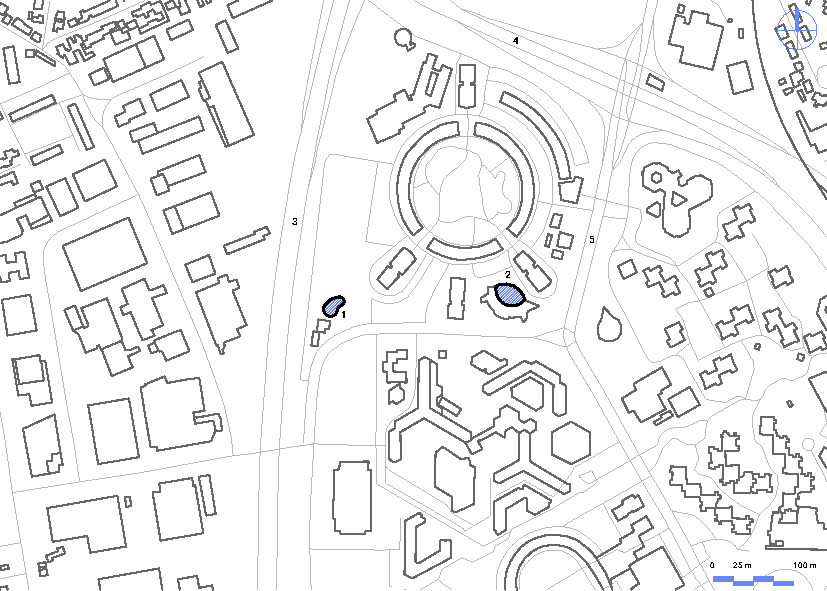
\includegraphics[width=\tmpwidth]{situation_map}}
		\intersectnode{PPtl |- CAtl}{Pt}
		\Photo[
			node=Pt,
			anchor=north west,
			xshift=0mm,
			gopt={width=\tmpwidth},
			]{situation_map}%
		\savenodes{A}
		\Photo[
			node=CAbr,
			anchor=south east,
			xshift=-2\PhotoBigSkip,
			% yshift=\PhotoSkip,
			gopt={height=3.75cm},
			]{form}%
		\savenodes{B}
		\intersectnode{CAtl |- Abr}{Pt}
		%%
		\PhotoCaptionRef[
			hrefnode=Atl,
			node=Atr,
			anchor=south east,
			yshift=\PhotoRefSkip,
			phantom=true,
			]{figure}{Situation map}{Situation map of the cathedrale}{fig:situation_map}
		\PhotoTextBox[
			node=Pt,
			anchor=north west,
			yshift=-\PhotoBigSkip,
			% width=6cm,
			border=false,
			]{%
				\figurecaption[The temporary gridshell (1) was built very close to the permanent cathedral (2). Remark that  the two buildings cover a quite similar projected area.]{fig:situation_map}
			}
		%%
		\PhotoCaptionRef[
			hrefnode=Btl,
			node=Bbr,
			anchor=north east,
			yshift=-\PhotoRefSkip,
			phantom=true,
			]{figure}{Architectural sketch}{Architectural sketch (T. Gray)}{fig:form}
		\PhotoTextBox[
			node=CAbl,
			anchor=south west,
			border=false,
			]{%
				\figurecaption[\raggedright Major and minor volumes are agglomerated into one volume. Here, the morphological register allowed by elastic gridshells appears to be relevant.]{fig:form}
			}
	}
}



\subsection{Context and challenges}
%----------------------------------------------
Creteil is a city of 90.000 inhabitants in the southeast suburb of Paris. Its urbanization began in the late 50’s, impelled by the French architect Charles-Gustave Stoskopf. In 1976 he designed \emph{Notre Dame of Créteil}, a modest catholic church made of concrete, which became a cathedral 10 years later (see item 2 in \cref{fig:situation_map}). Recently, the diocese of Créteil has undertaken a major architectural redevelopment project of its cathedral, including a timber shell covering the religious area and the creation of a new cultural area. Once transformed, the edifice shall be more visible, more hospitable and livelier for citizens. Inevitably, such a molt takes time and a temporary place of worship was required to ensure liturgical services during the two-years work. In November 2011, T/E/S/S, the structural design office in charge of the cathedral renovation project, made an ambitious proposal to the diocese~: based on a previous successful experience – the construction of a composite gridshell for the festival Solidays \cite{Baverel2012} – T/E/S/S suggested that rather installing a basic tent, the parishioners should construct themselves a temporary cathedral.\footnote{See the video of the construction of Solidays' gridshell here : \url{https://youtu.be/24LLfcVIZWw}.}\textsuperscript{,}\footnote{See the video of the construction of Creteil's gridshell here : \url{https://youtu.be/jLq-UfOdnQQ}.}

% \begin{figure}[t]
% 	\centering
% %	\begin{fullpage}
% 		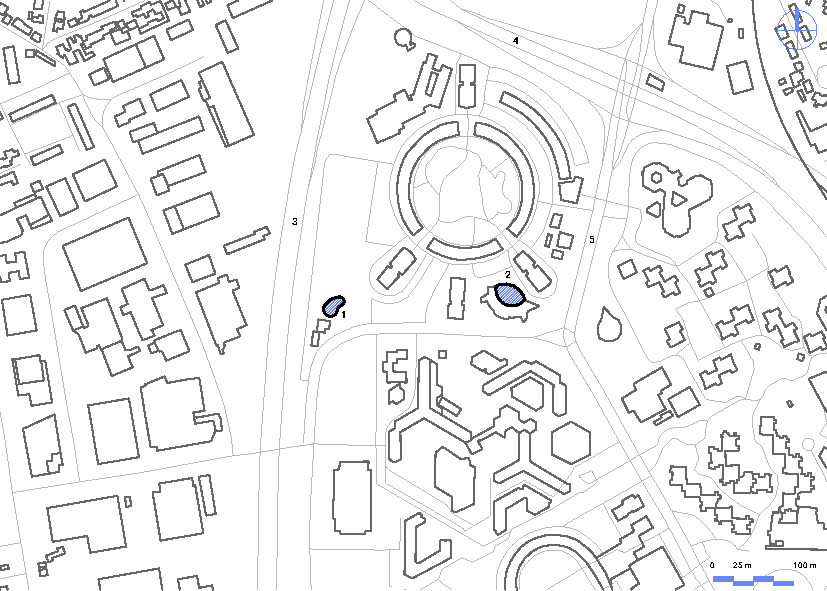
\includegraphics[width=1\textwidth]{situation_map}
% 		\caption[Situation map]{Situation map. The temporary gridshell (1) was built very close to the permanent cathedral (2). Remark that  the two buildings cover a quite similar projected area.}
% 		\label{fig:situation_map}
% %	\end{fullpage}
% \end{figure}

\subsection{Architectural considerations on the form}
%------------------------------------------------------------------
The origin of this building form was driven by two objectives, that is, to provide a variety of appropriate internal spaces within which the community could assemble, and to provide an externally welcoming and visually interesting form. According to the architect Tom Gray, today, the internal organization of a roman catholic church is in large part driven by the post Vatican II vision of a religious celebration being a collective gathering of the community around the Eucharist, center of spiritual life. A circular seating arrangement is often considered the most convivial form to create a sense of belonging while minimizing a sense of hierarchy. However the community is not only using the building for religious celebration but also for encounters on a more informal manner, for example spontaneous gatherings after religious ceremonies. In the early Roman church, such gathering of the community was facilitated by the presence of an anti-space to the main space called a \emph{narthex}, through which one passed on entering the church. It was therefore felt appropriate that the formal freedom which the gridshell system offered would be used to explore forms composed of an agglomeration of major and a minor volumes which contain the two functions~: formal and informal gatherings (see item 1 and 2 in \cref{fig:form}).

Formal explorations were undertaken using modeling clay. The final form is based loosely on two adjacent semi spherical volumes of different size, which are merged into one complex form. Externally the fear of the design team was that the totally convex blob form could look intimidating. It was therefore decided that the two spherical virtual forms, which would be joined to make the final form, would be arranged not in a symmetrical axial manner, but in an asymmetrical curved composition. The resulting form seen in plan is convex on one side and concave on the other. The concave form in plan allows for double curvature to be introduced into what would be otherwise a simpler blob and gives sensuality and visual interest to the building.

% \begin{figure}[t]
% 	\centering
% 	\begin{fullpage}
% 		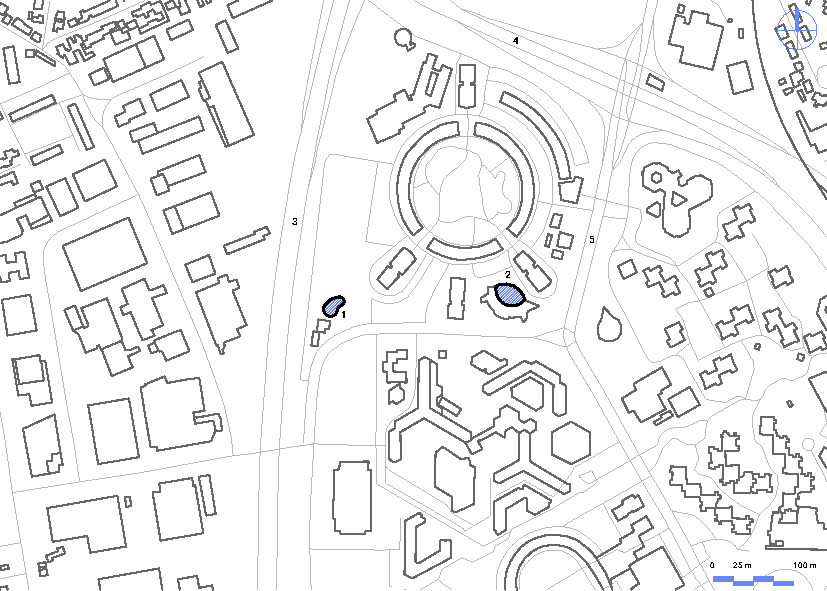
\includegraphics[width=1\textwidth]{situation_map}
% 		\caption[Situation map]{Situation map. The temporary gridshell (1) was built very close to the permanent cathedral (2). Remark that  the two buildings cover a quite similar projected area.}\label{fig:situation_map}
% 		\vspace{1.5cm}
% 		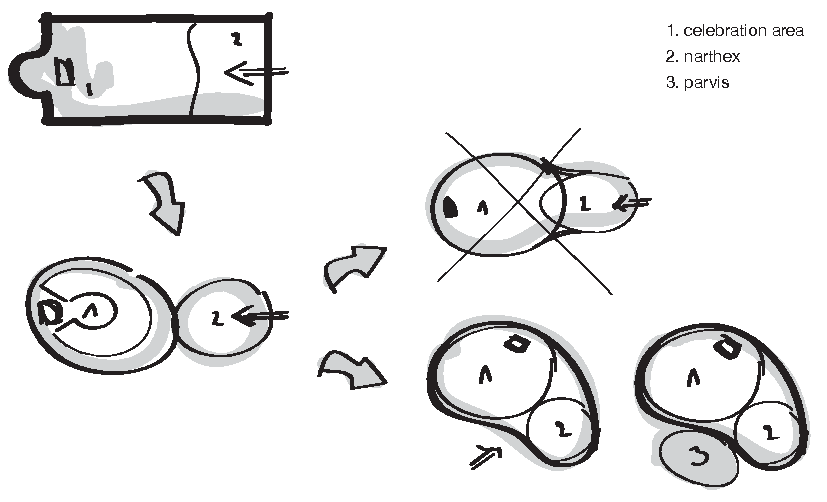
\includegraphics[width=0.7\textwidth]{form}
% 		\caption[Architectural sketch]{Architectural sketch (T. Gray). Major and minor volumes are agglomerated into one volume. Here, the morphological register allowed by elastic gridshells appears to be relevant.}\label{fig:form}
% 	\end{fullpage}
% \end{figure}

% \begin{figure}[p]
% 	%
%      	\centering
% 	\begin{leftfullpage}
% 		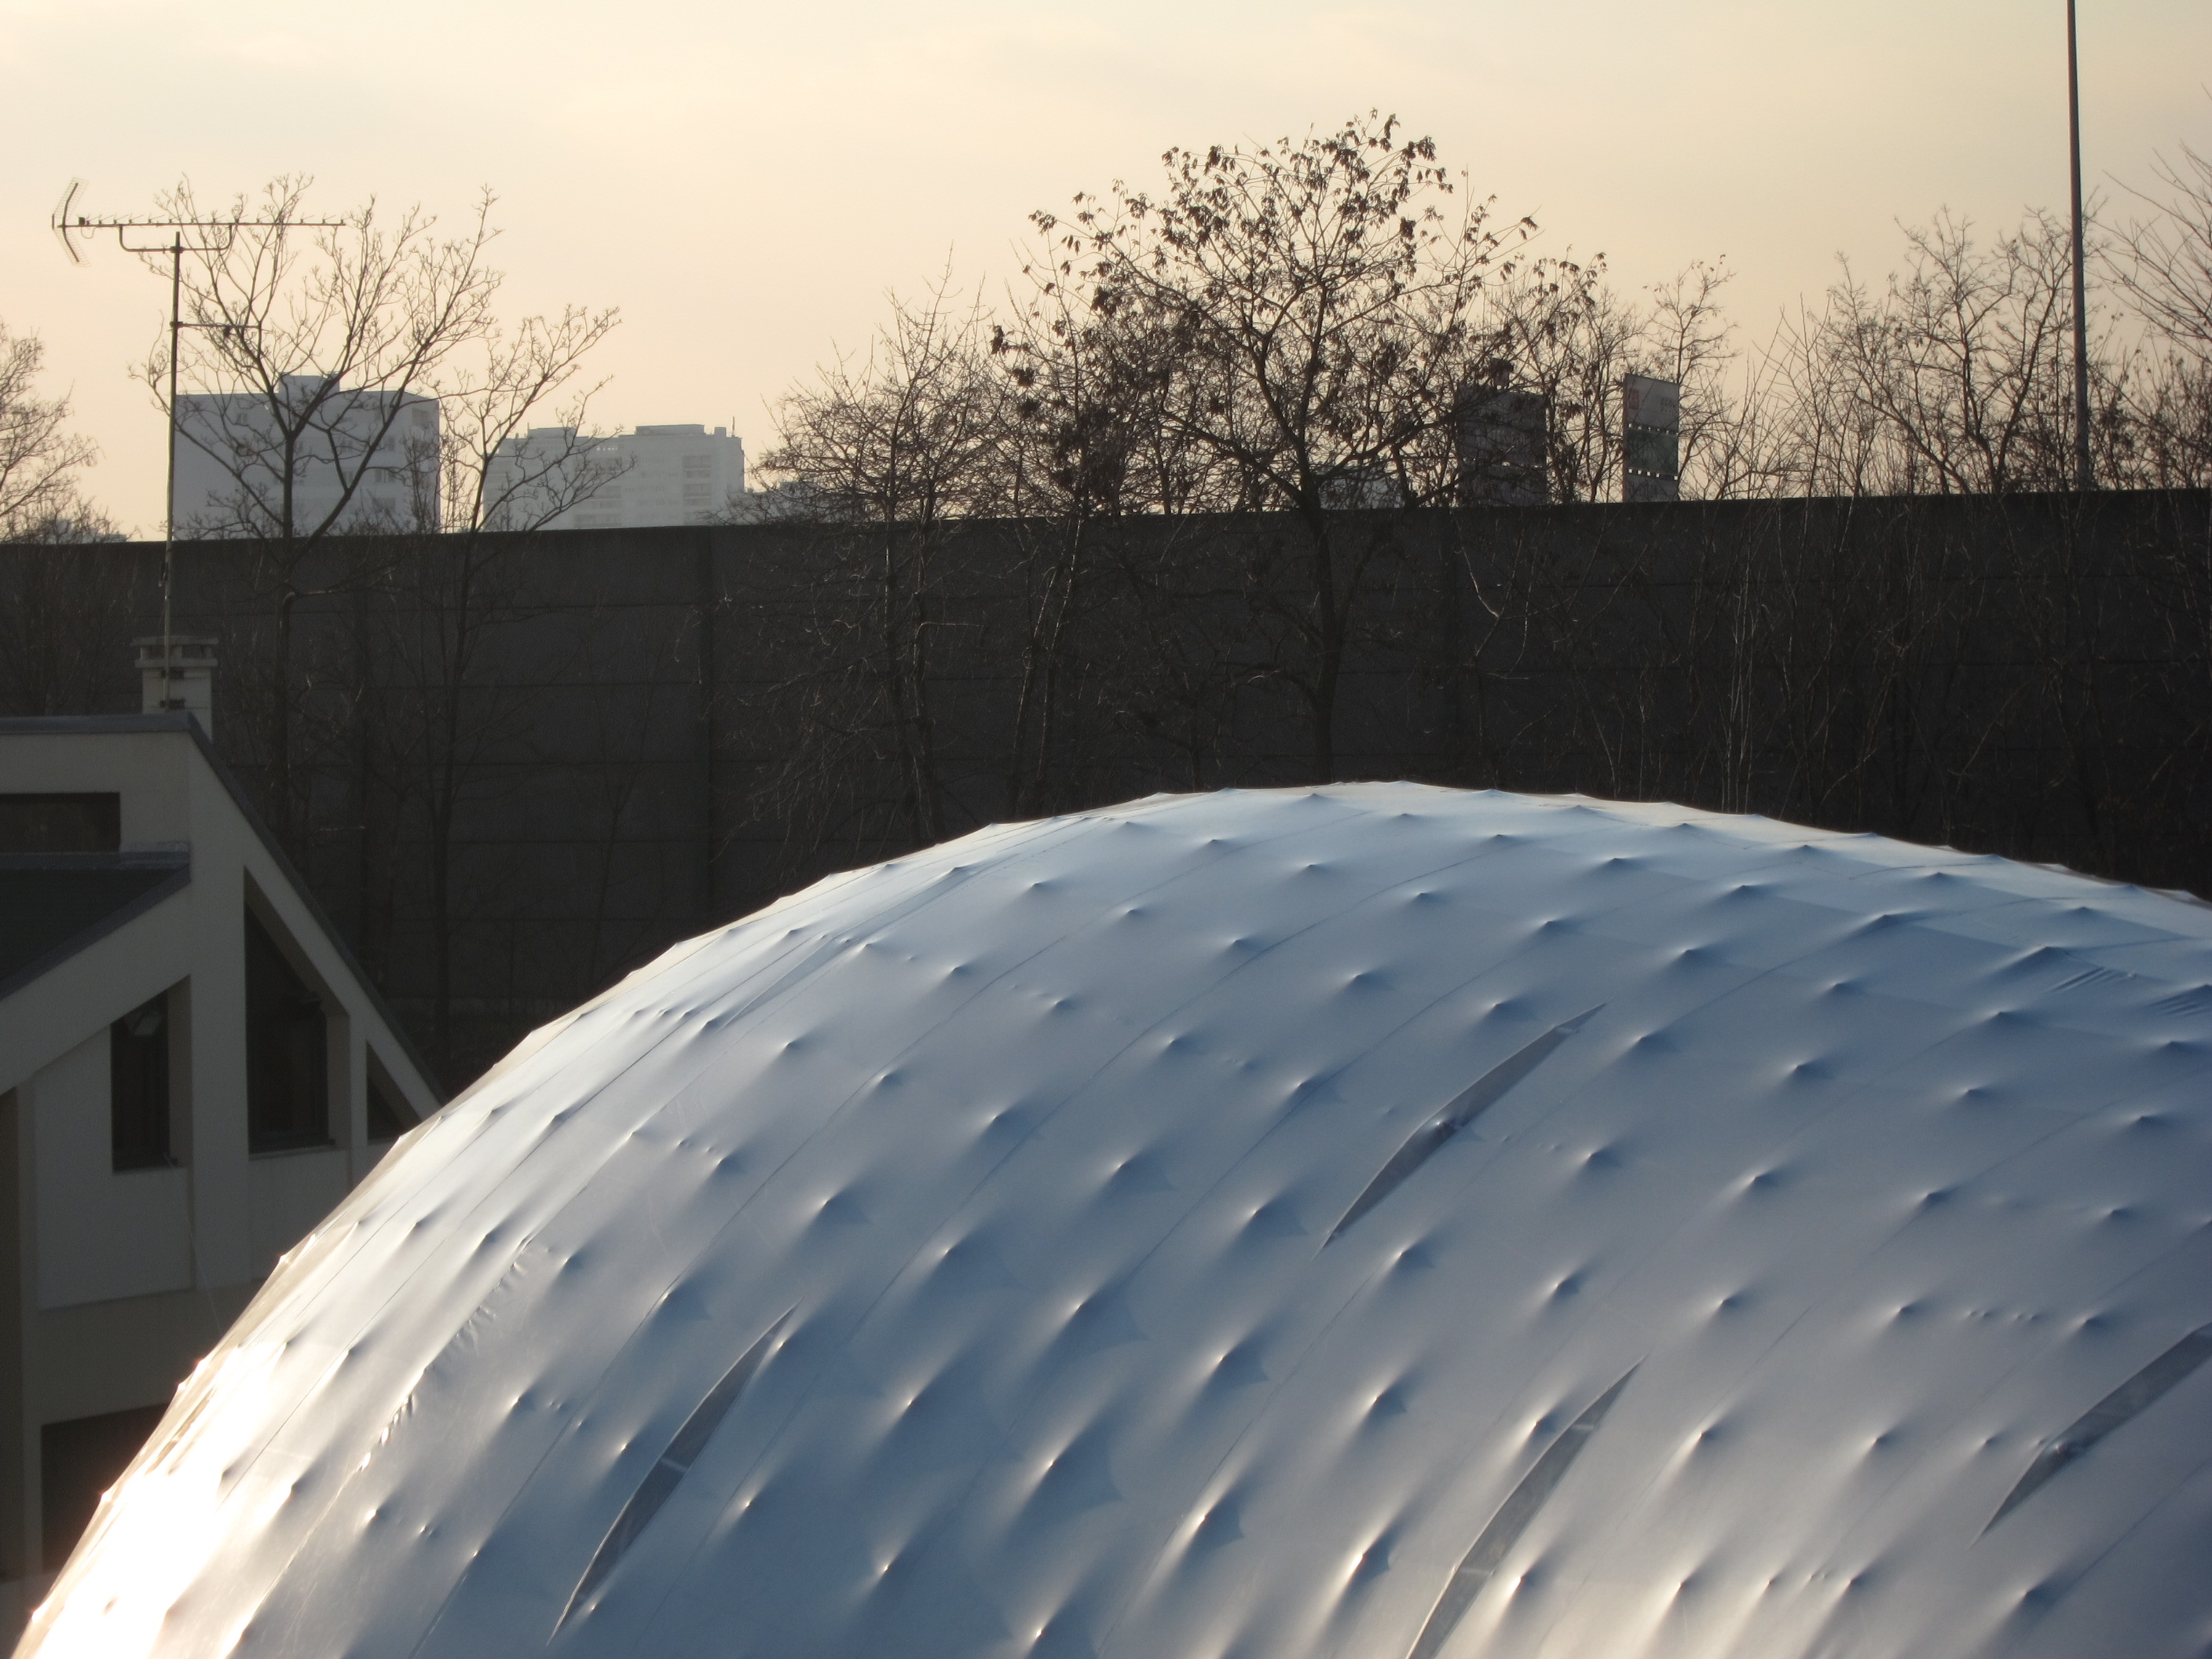
\includegraphics[width=0.80\textwidth]{gs_ext.jpg}
% 		\caption[Exterior view]{Exterior view. The connections mark the fabric suggesting the interior grid structure. This texture enriches the perception of the building viewed from the outside and creates effects with the light reflections -- \textcopyright~L. du Peloux for T/E/S/S.}
% 		\label{fig:gs_ext}
% 		\vspace{1cm}
% 		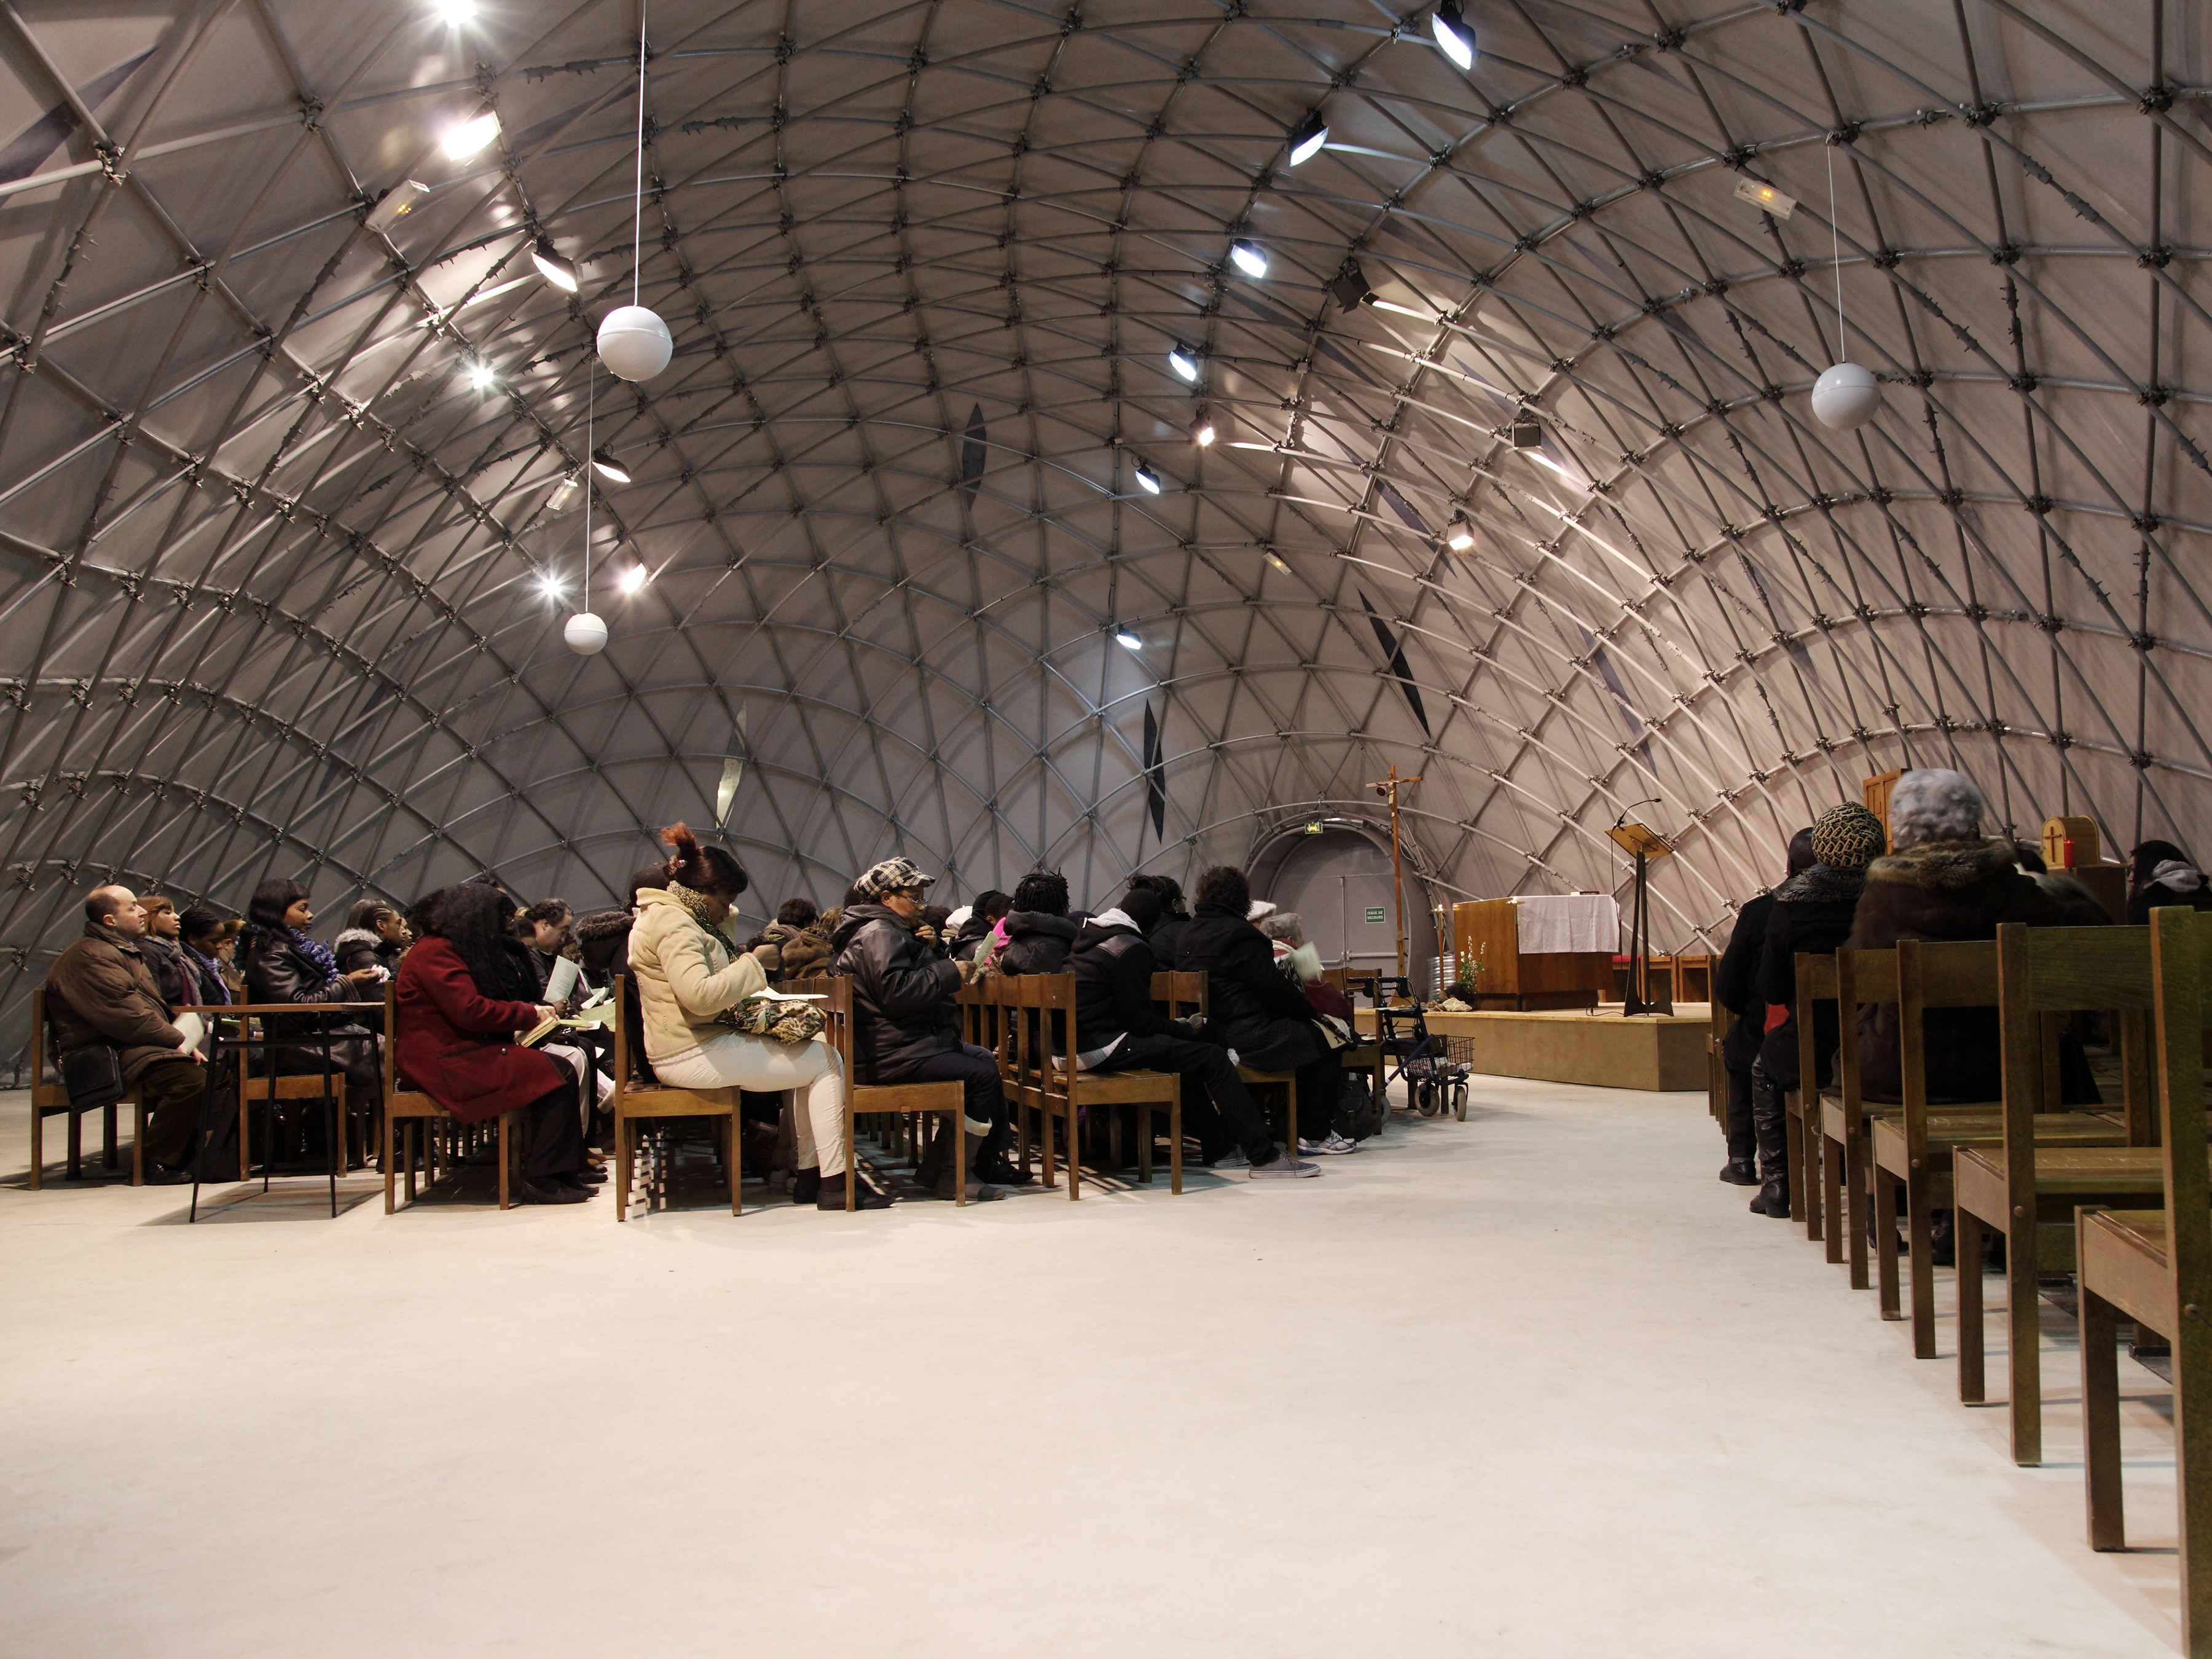
\includegraphics[width=0.80\textwidth]{gs_int.jpg}\label{fig:gs_int}
% 		\caption[Interior view]{Interior view. The grid pattern highlights the lightness of the structure and gives its tempo to the internal space. Lines converge to the altar, the heart of the liturgical area where the mass is offered on -- \textcopyright~C. Moissinac for T/E/S/S.}
% 		\vspace{20pt}
% 	\end{leftfullpage}
% \end{figure}

% \begin{figure}[p]
%      	\centering
% 	\begin{fullpage}
% 		%
% 		\subfloat[][Exterior]{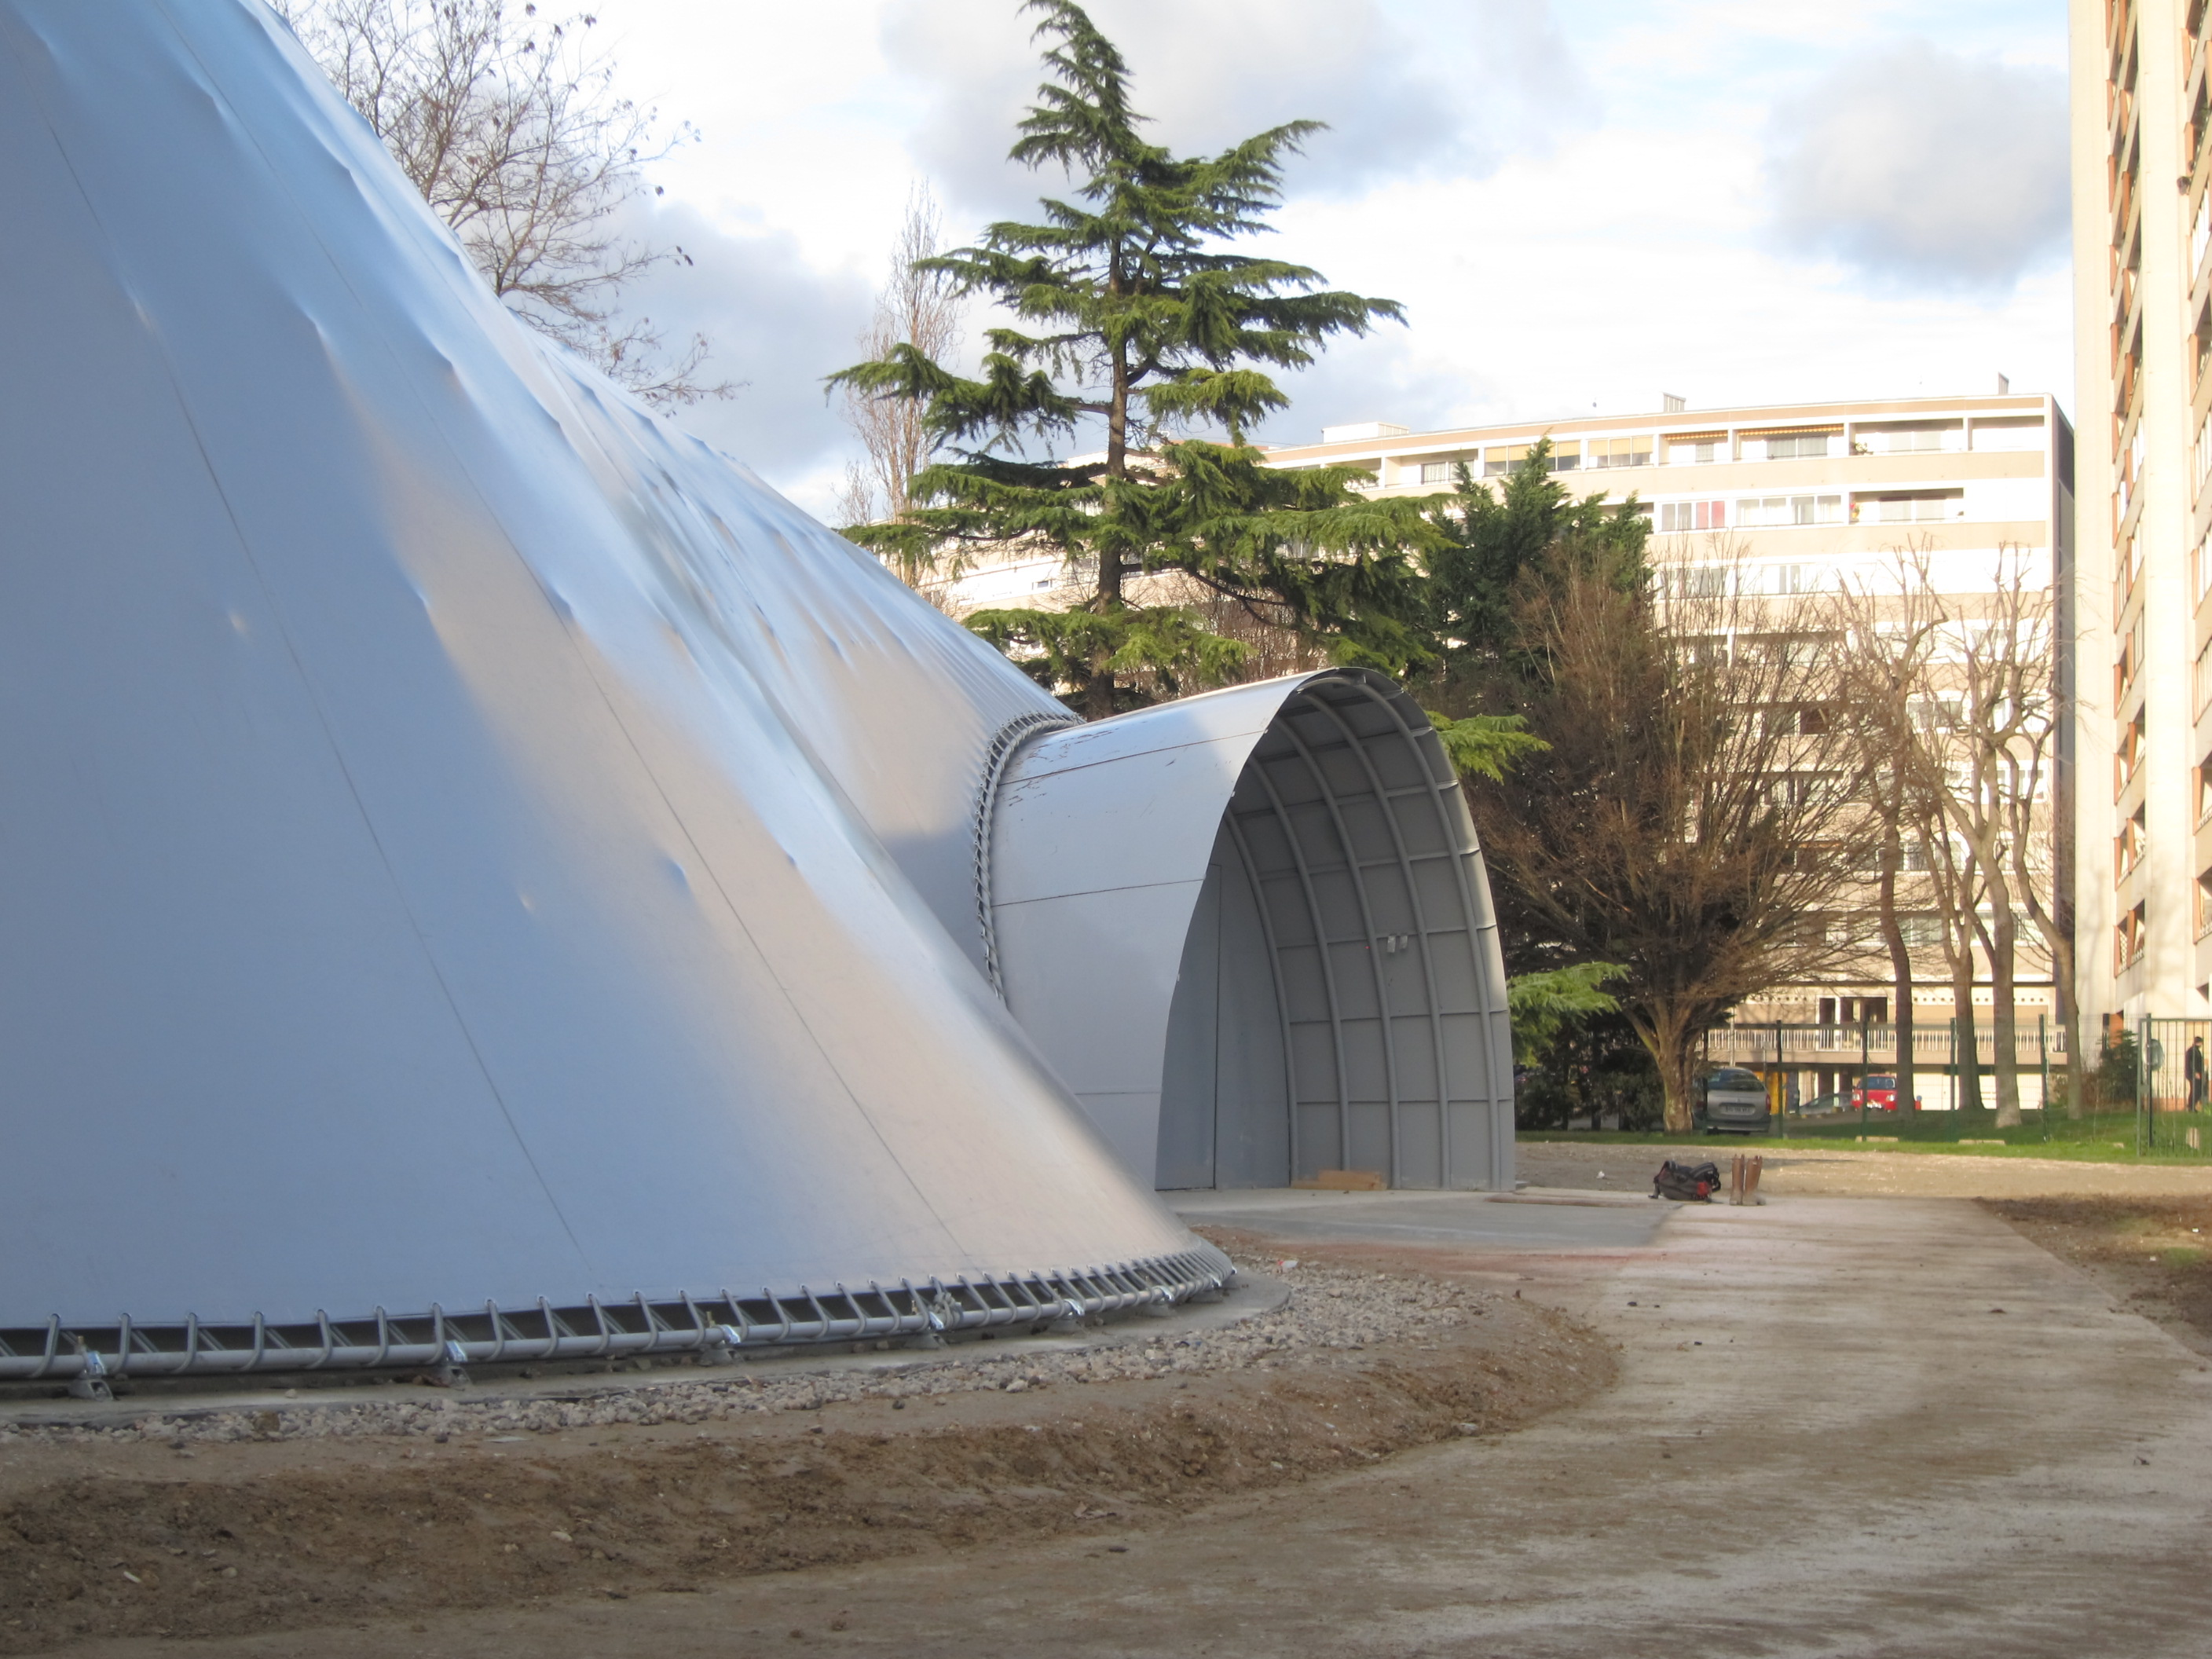
\includegraphics[width=0.48\textwidth]{door_ext.jpg}\label{fig:door_ext}}
% 		\hspace*{\fill}
% 		\subfloat[][Interior]{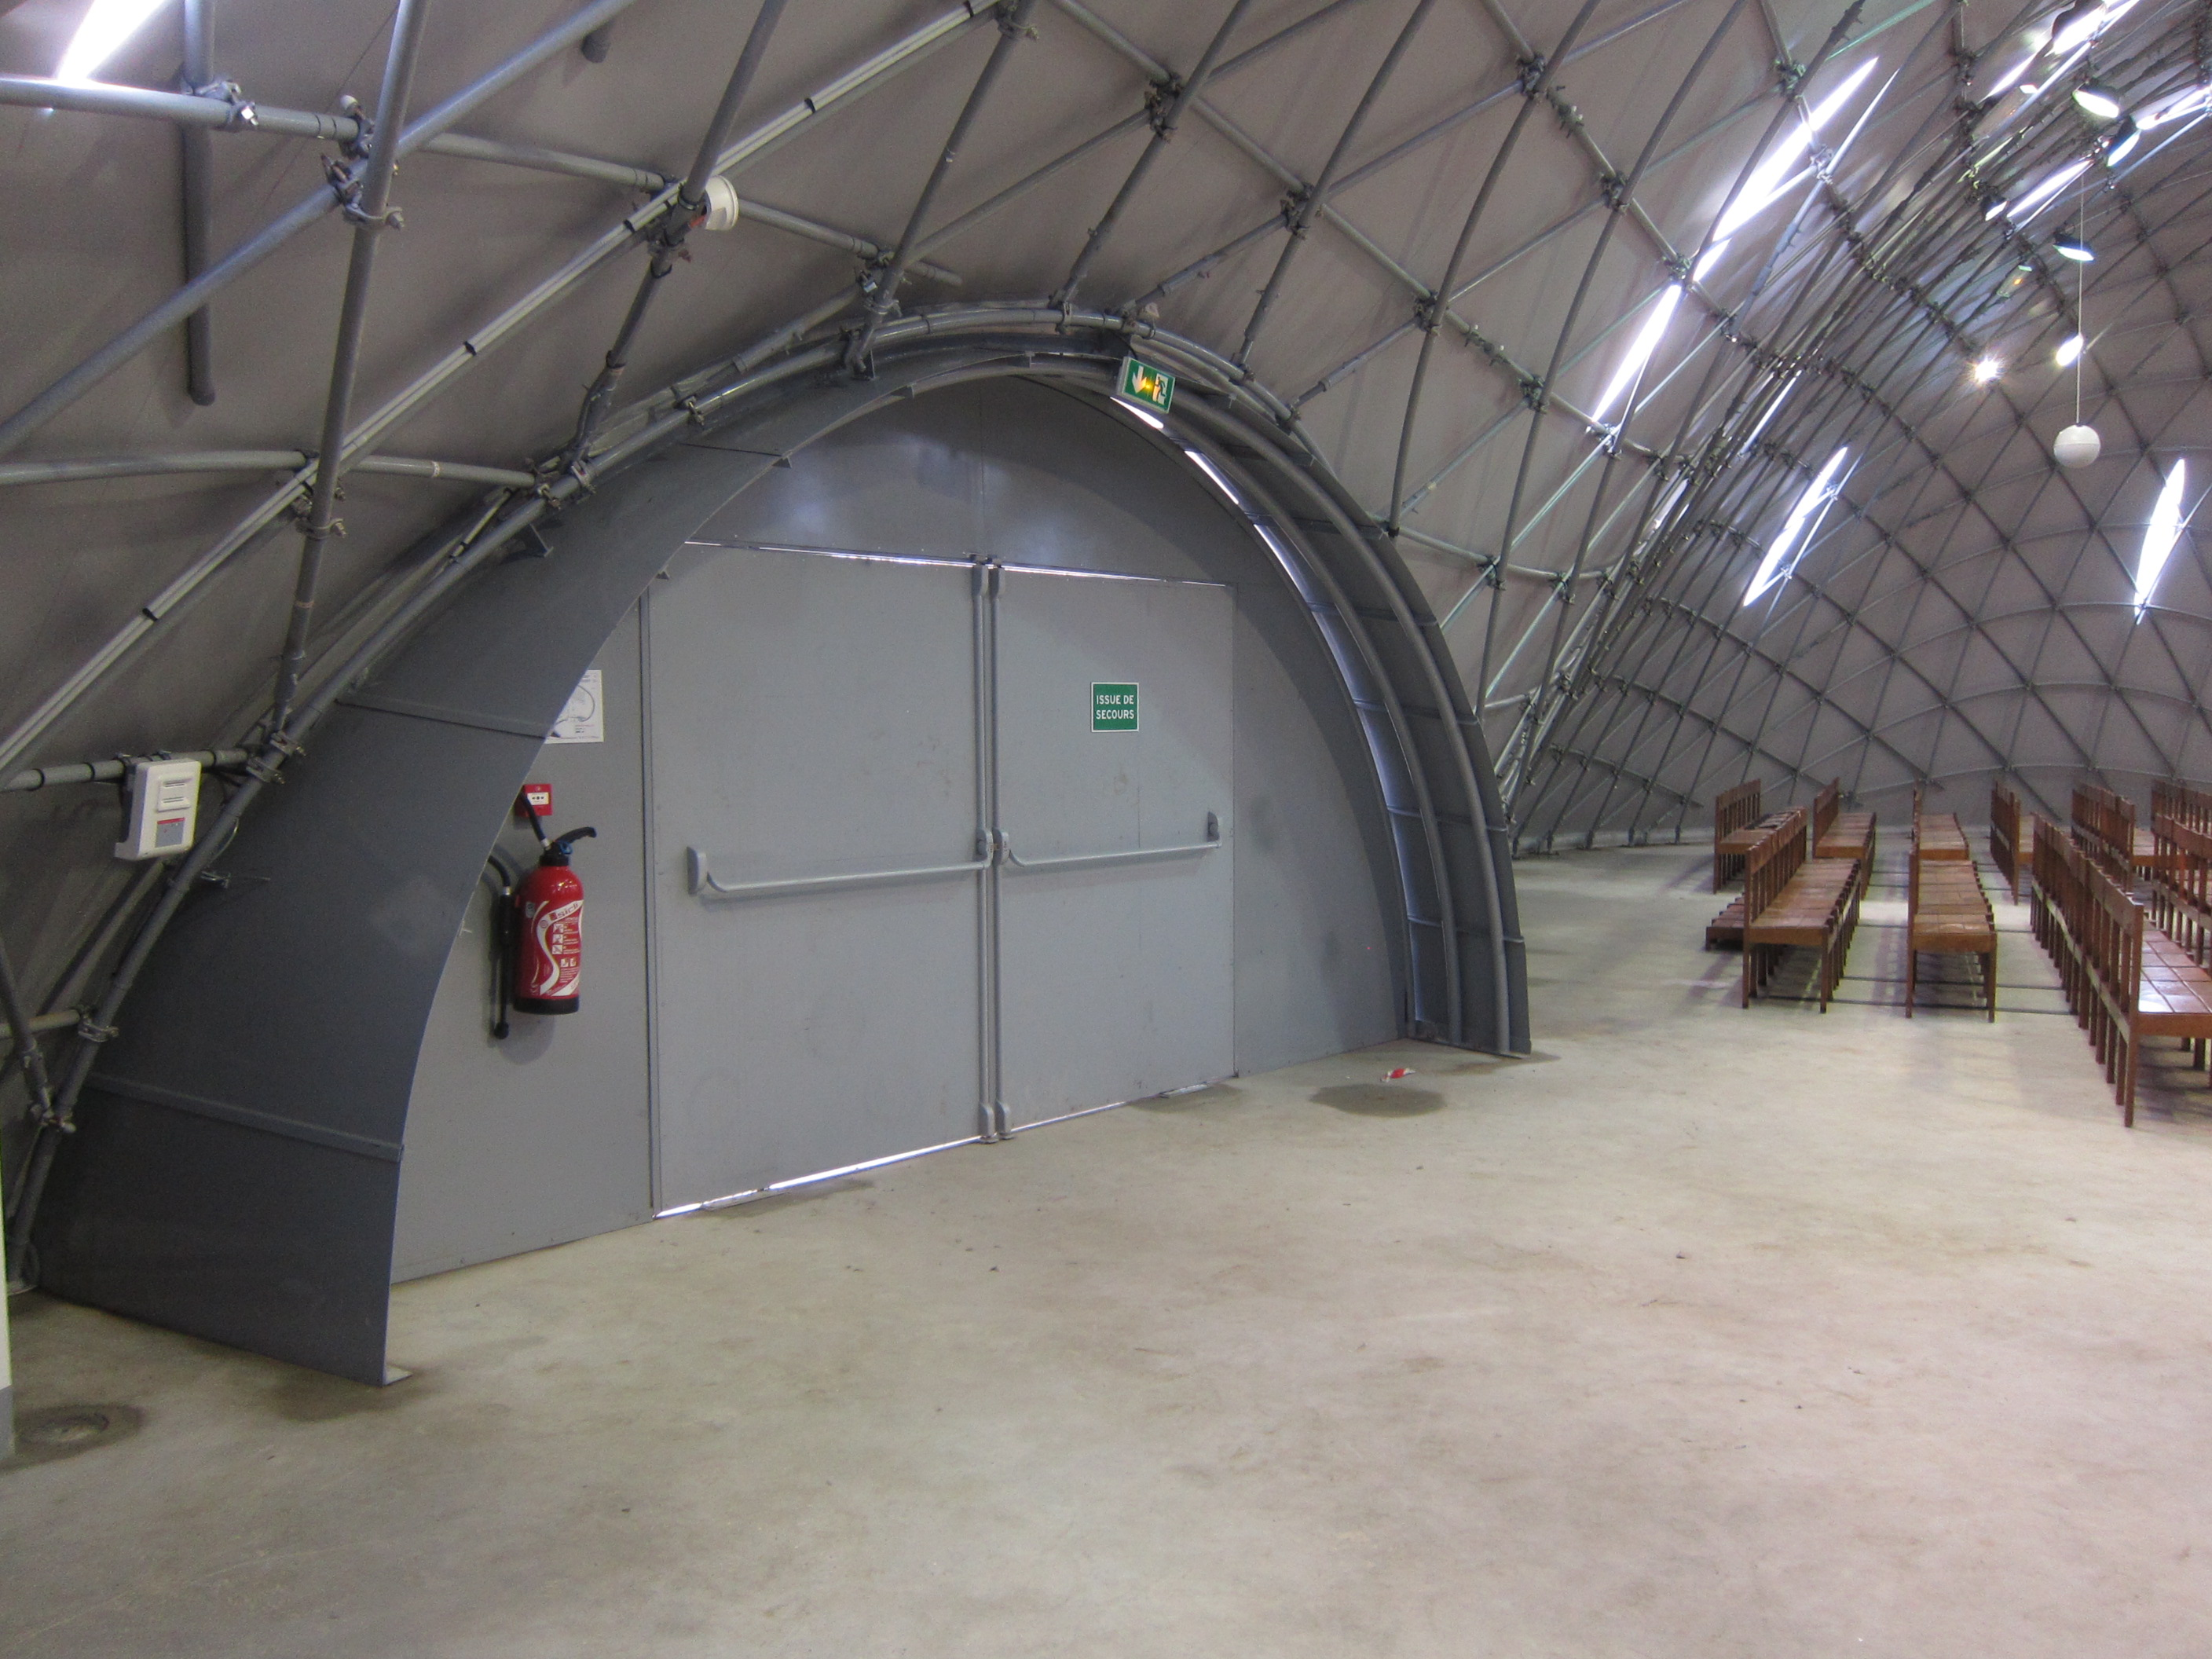
\includegraphics[width=0.48\textwidth]{door_int.jpg}\label{fig:door_int}}
% 		\vspace{10pt}
% 		\caption[Entrance]{Entrance. Two steel doors allow the entrance inside the building.}
% 		\label{fig:door}
% 		%
%      		\vspace{1cm}
% 		%
% 		\subfloat[][Swivel coupler]{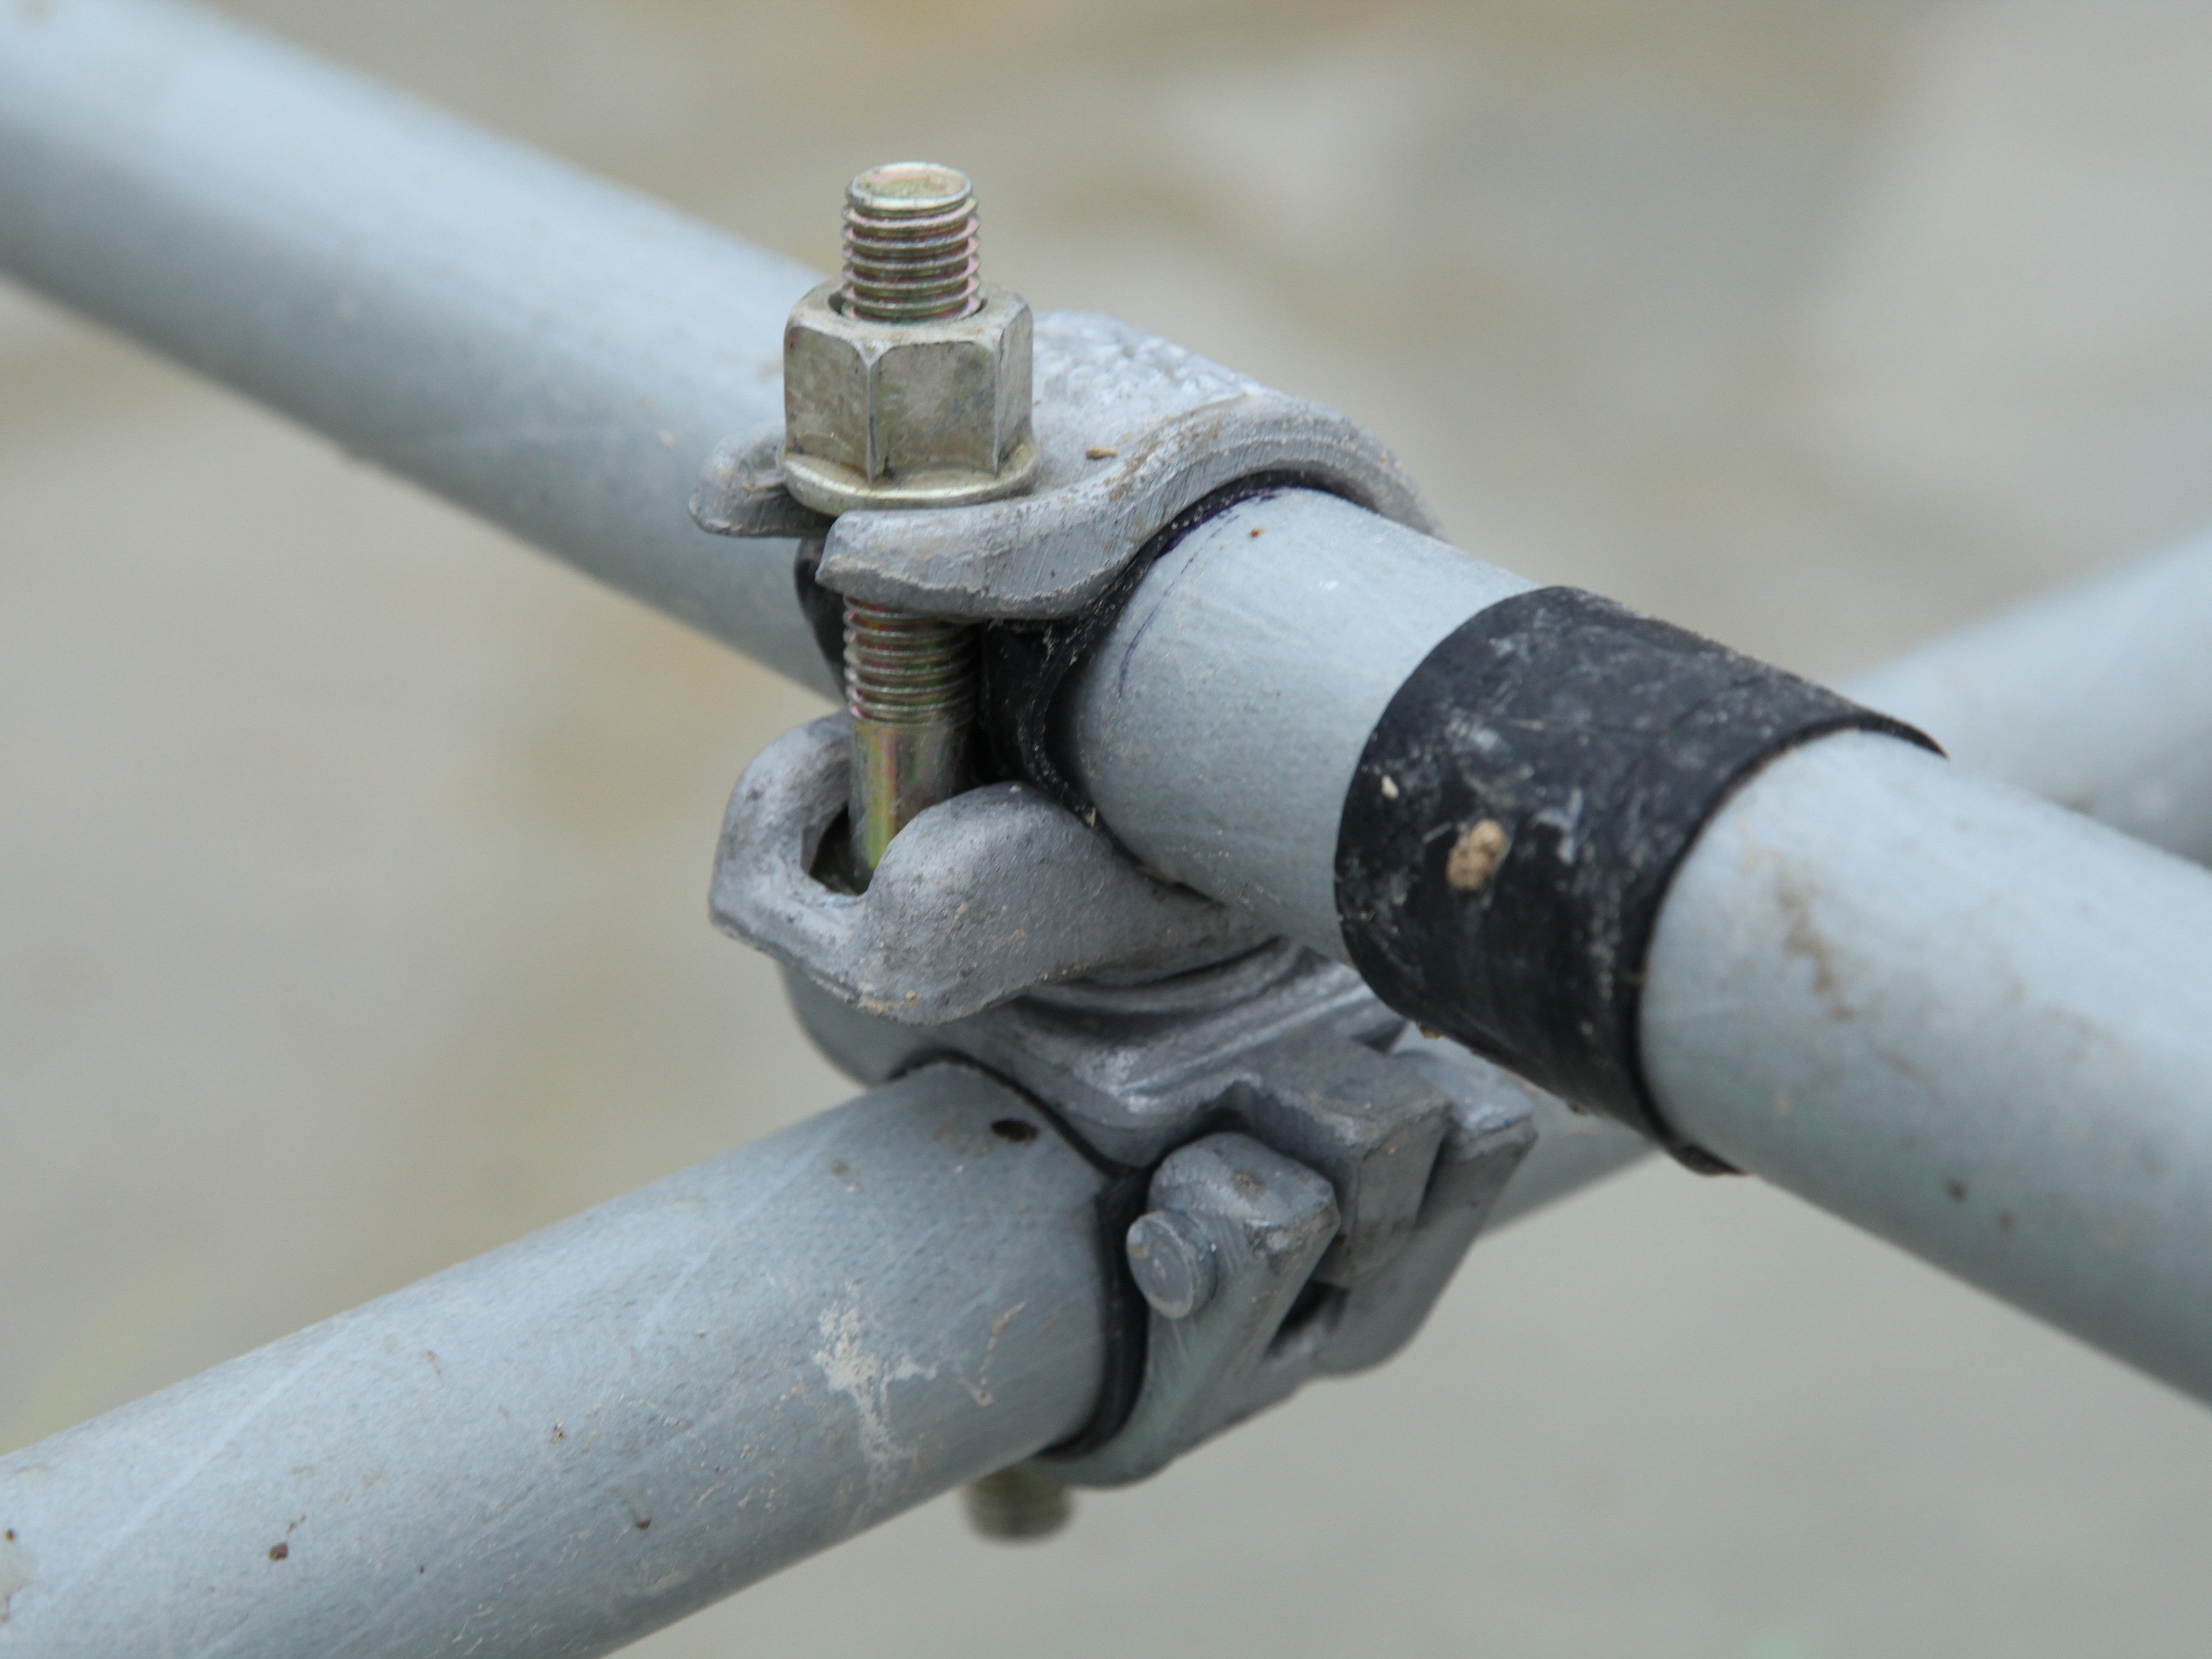
\includegraphics[width=0.48\textwidth]{swivel.jpg}\label{fig:swivel}}
% 		\hspace*{\fill}
% 		\subfloat[][Sleeve system]{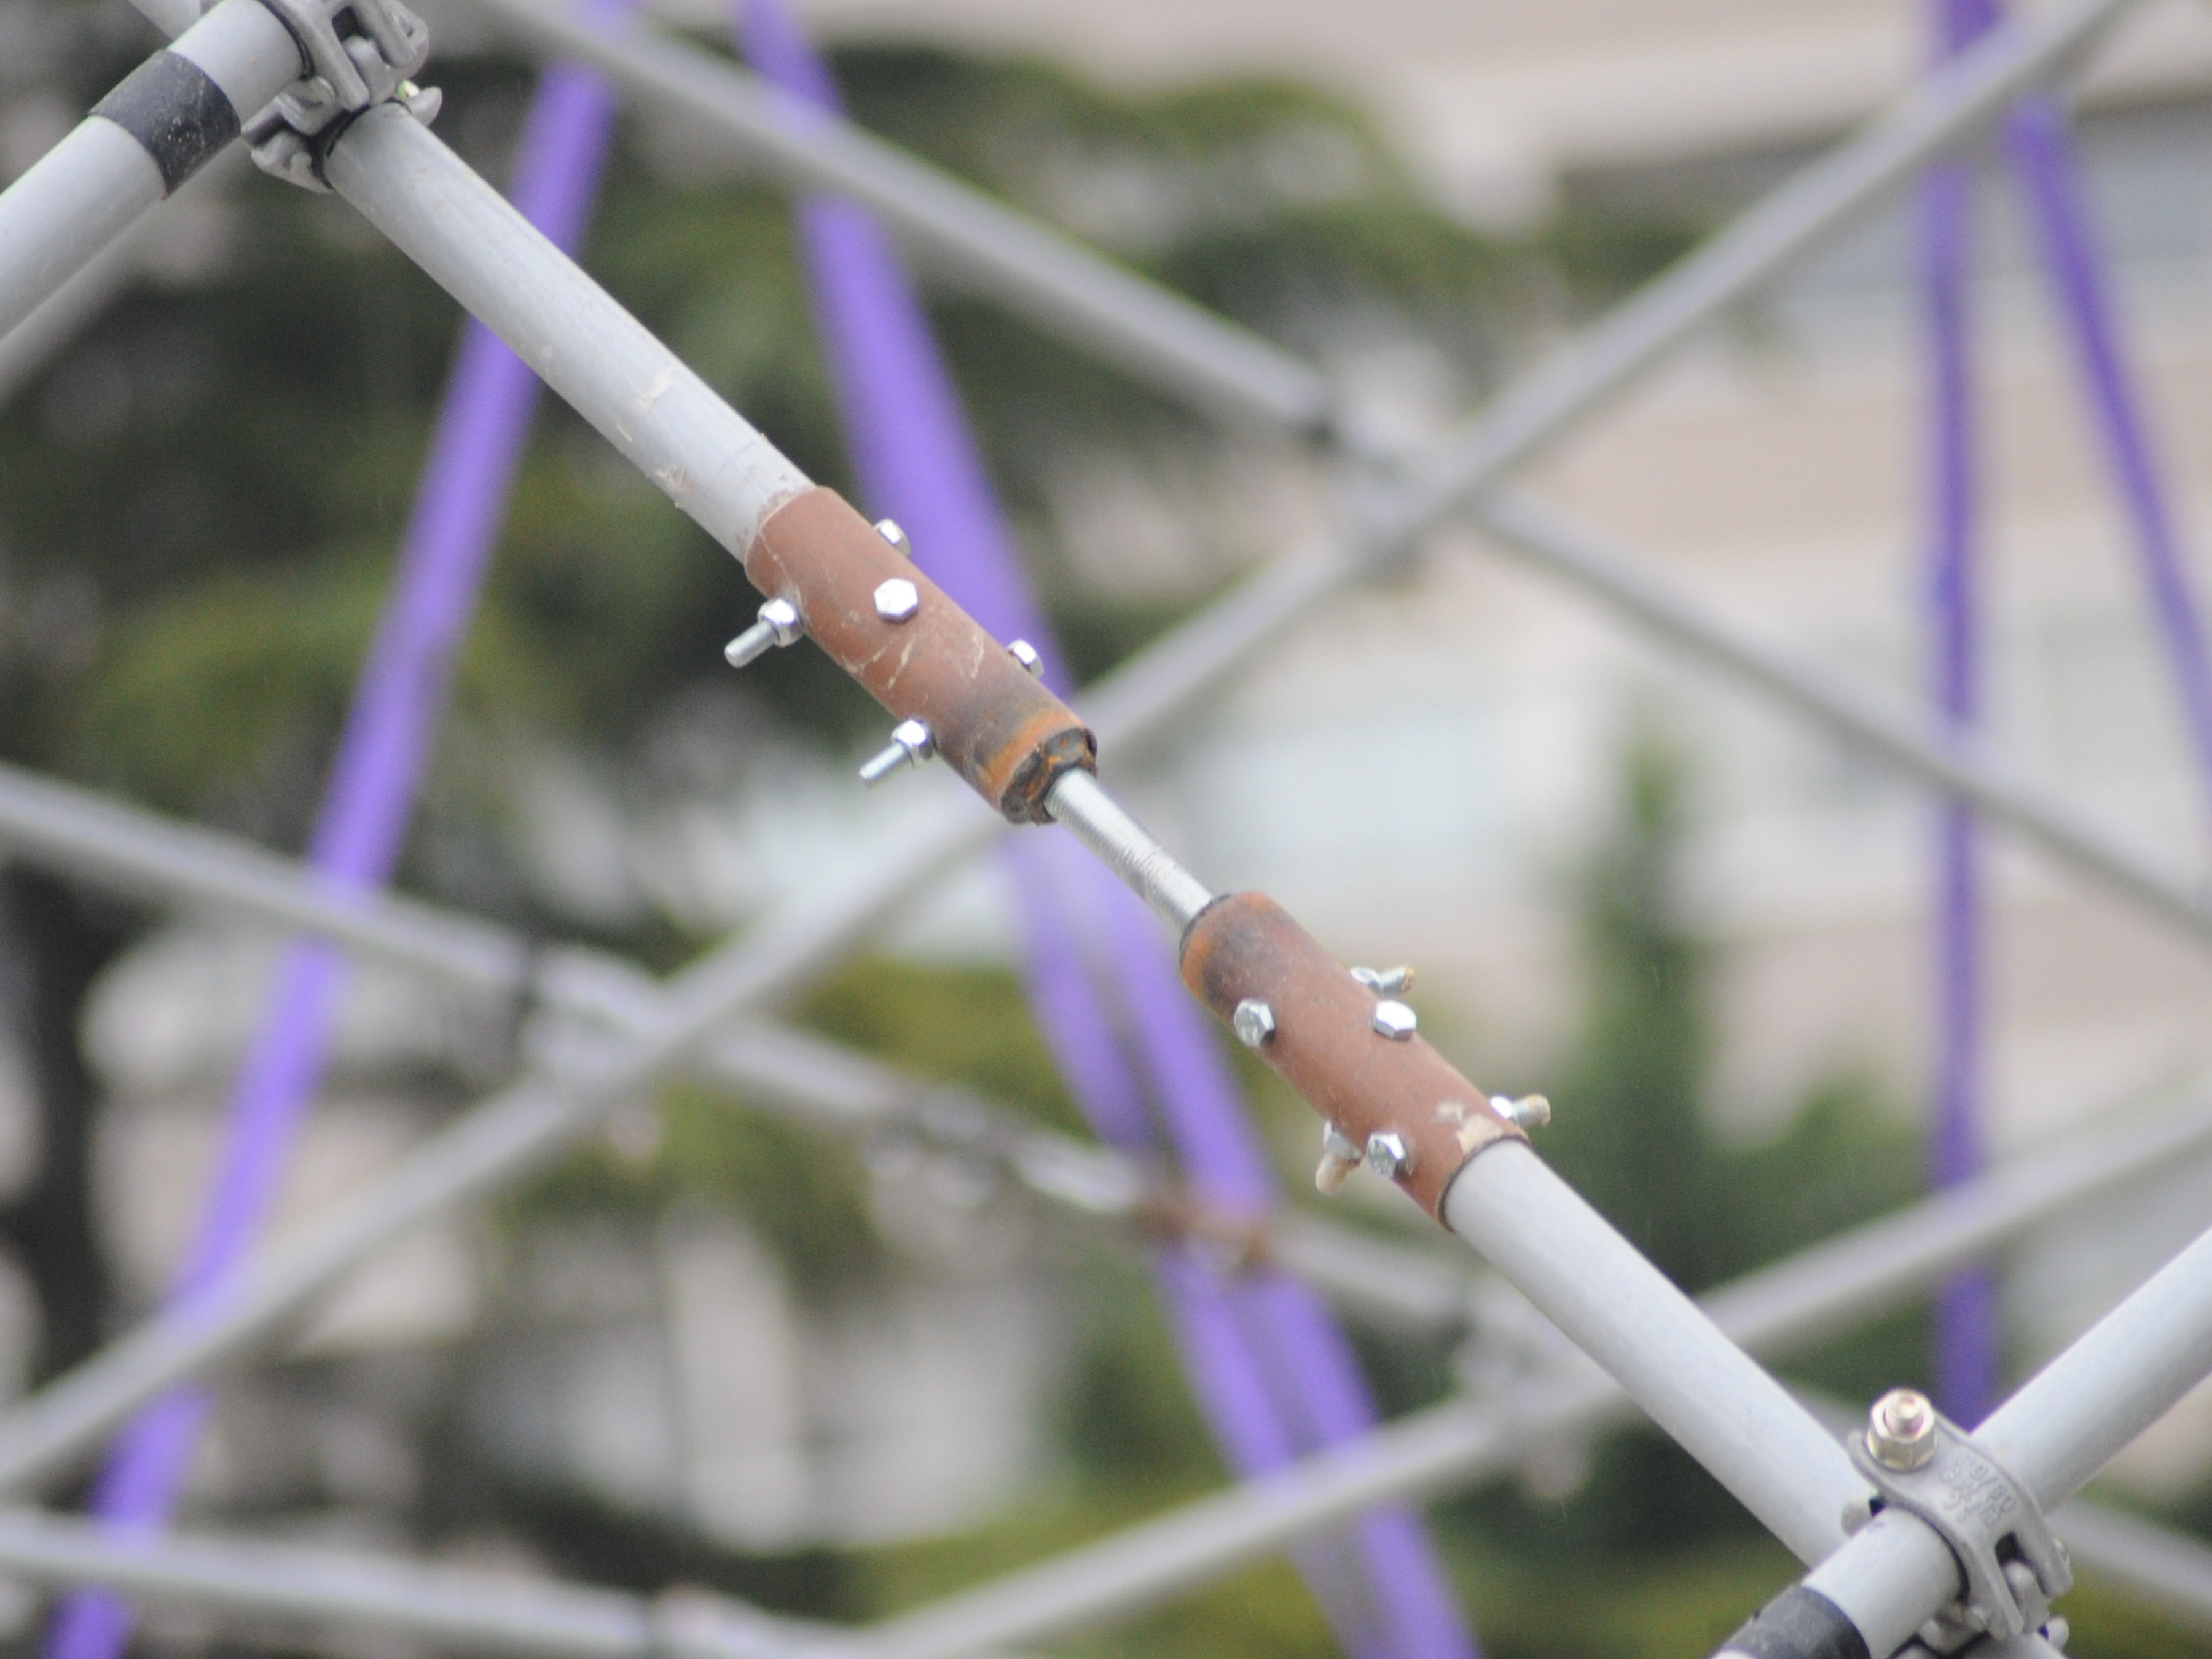
\includegraphics[width=0.48\textwidth]{sleeve.jpg}\label{fig:sleeve}} \\
% 		%
% 		\subfloat[][Ground anchorage]{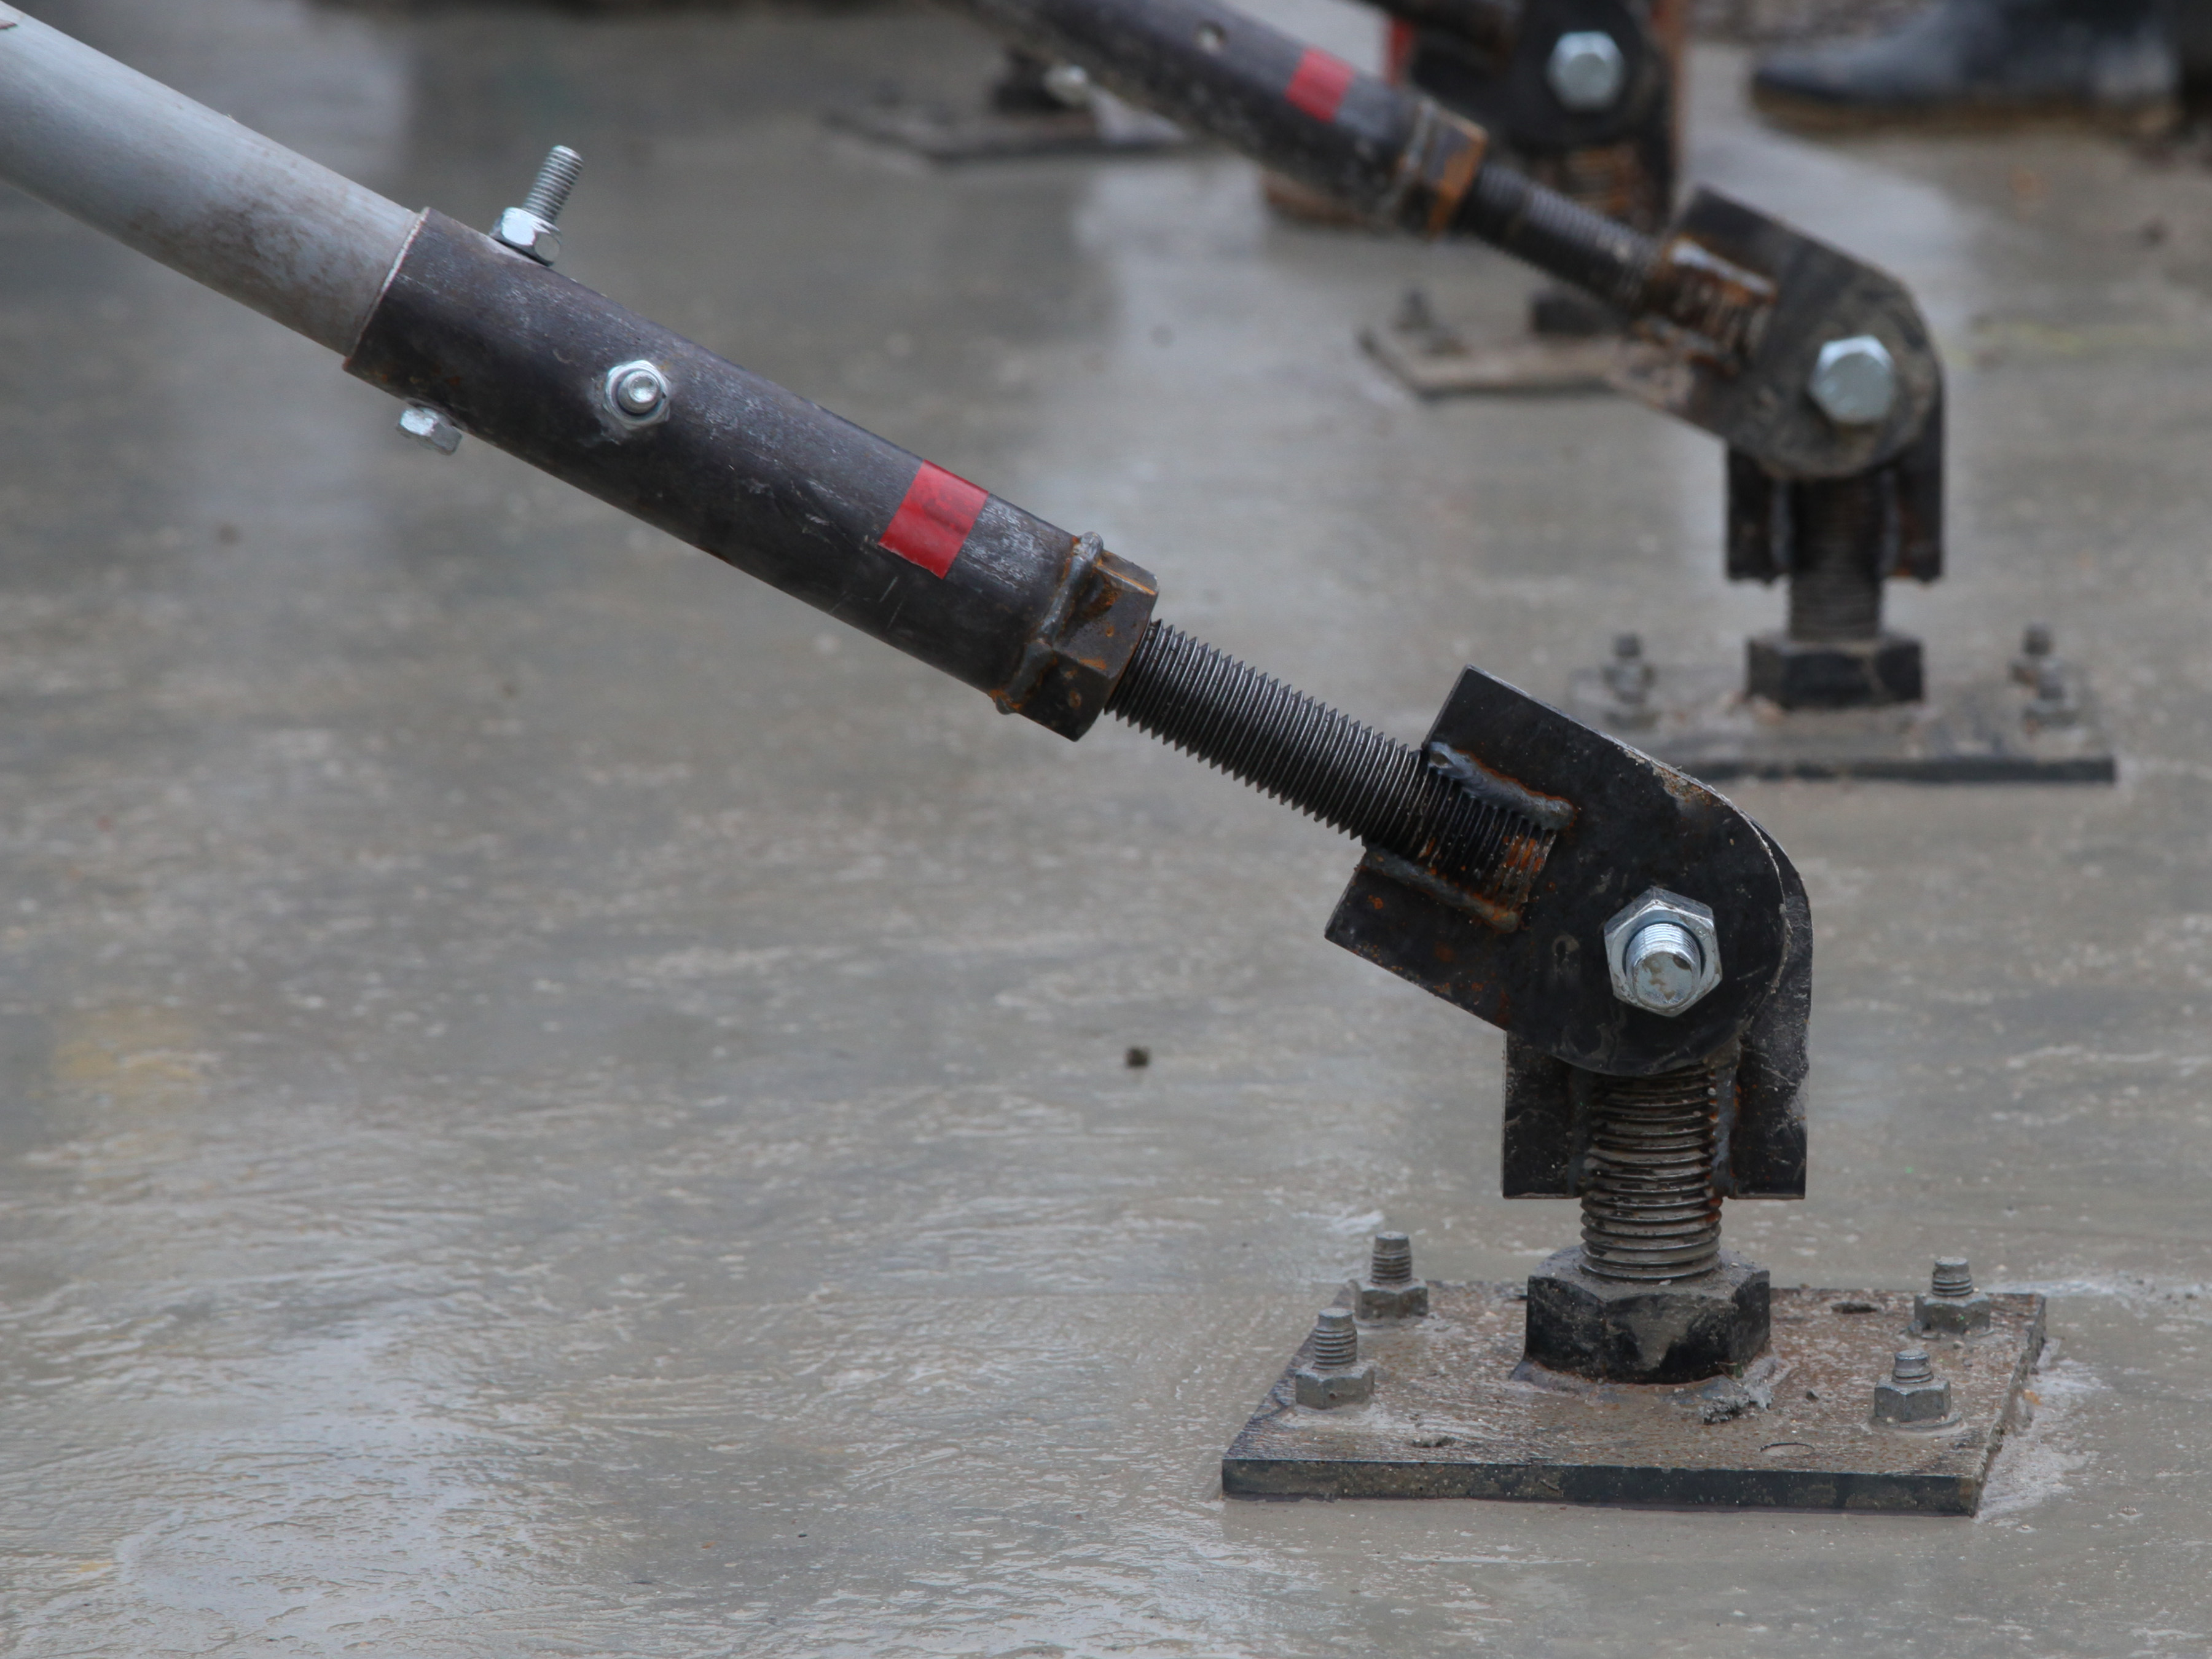
\includegraphics[width=0.48\textwidth]{anchorage.jpg}\label{fig:anchorage}}
% 		\hspace*{\fill}
% 		\subfloat[][Lacing rod]{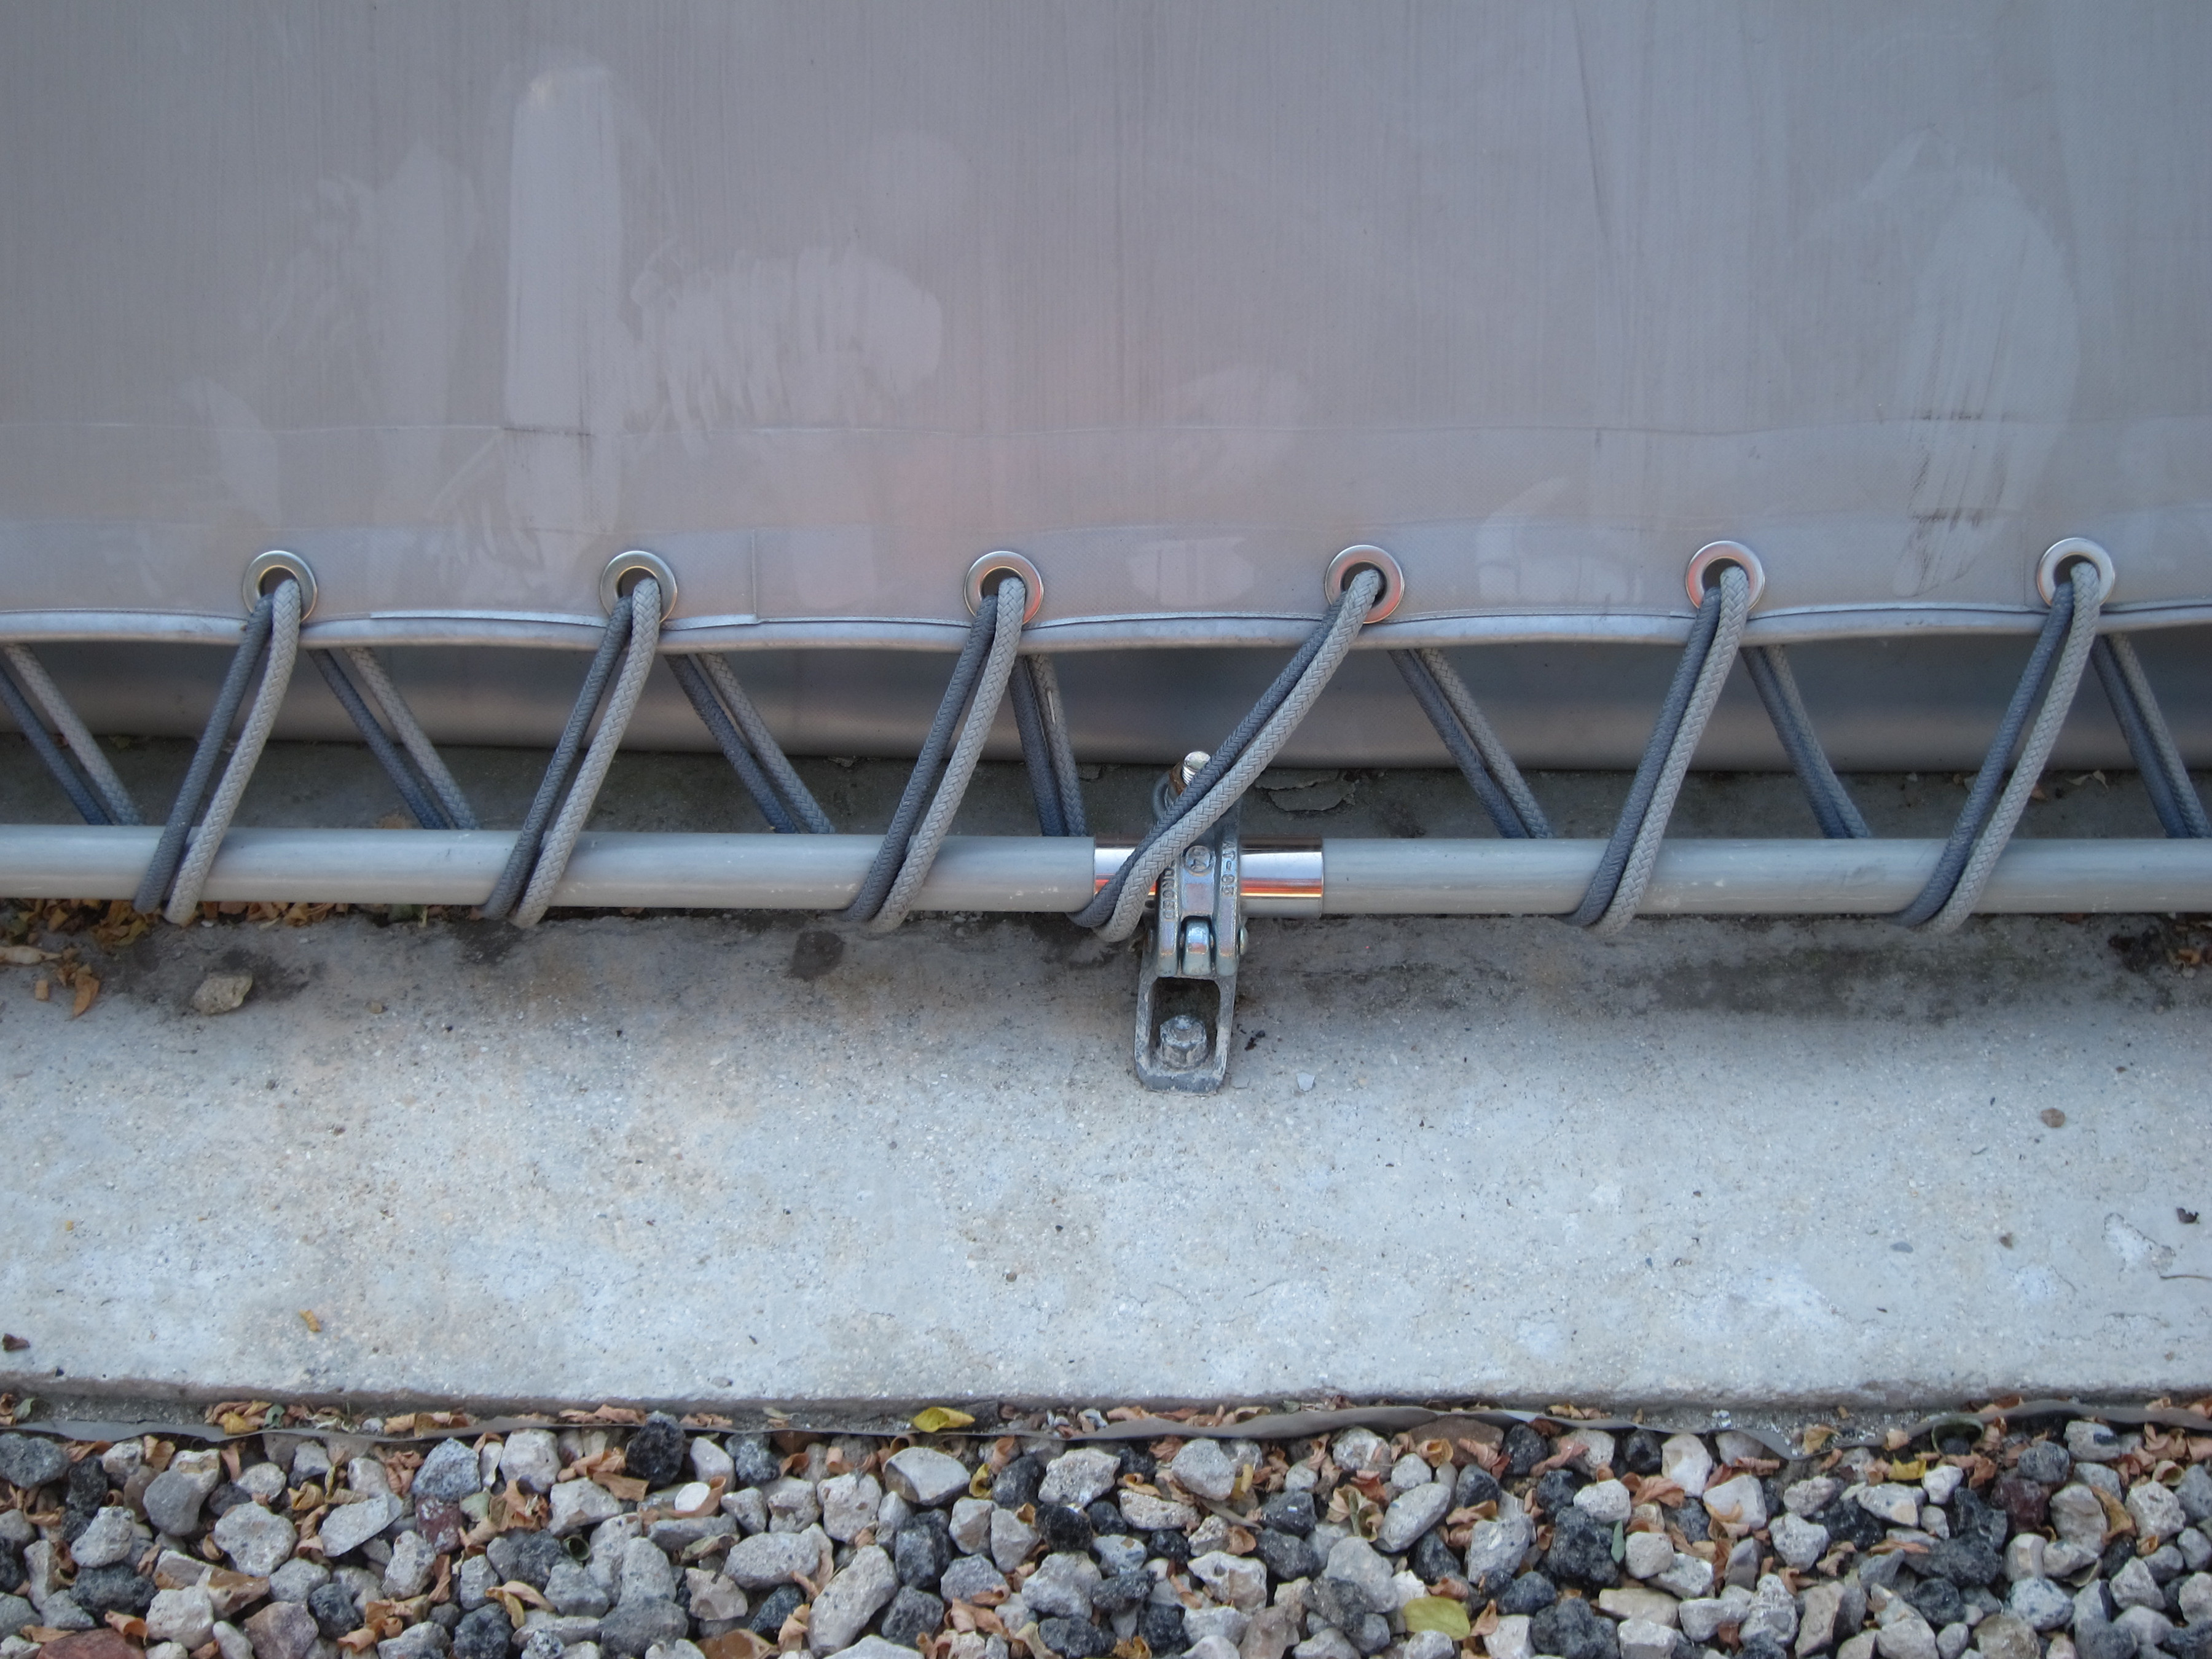
\includegraphics[width=0.48\textwidth]{edge.jpg}\label{fig:edge}} \\
% 		%
% 		\vspace{10pt}
% 		\caption[Key elements of the structural system]{Key elements of the structural system.}
% 		\label{fig:parts}
% 	\end{fullpage}
% \end{figure}

\subsection{Placing of the building on the site}
The temporary cathedral is located on a land owned by the municipality, which is used for sporting and other communal gatherings. The curve in the building defines an external area where the church community could meet in the open air and this is where the entrance to the church is situated. The building was positioned on the site so that the entrance addresses a grass planted area forming a garden forecourt or “parvis” (see item 3 in \cref{fig:form}). A service building housing plant, toilets and vestry are housed in a port cabin positioned to the rear of the building (see \cref{fig:plan_view}).

\subsection{Entrance}
It is formally quite difficult to integrate doors, which must be verticals, into a complex geometry. Either the gridshell could be deformed to accommodate the geometrical requirements of doors, or the doors could be integrated into an independent form. The latter approach was chosen. In looking for forms to house the doors, reference was made to the conical monumental doorways with rings of concentric decoration, which welcome the faithful to romanesque and gothic churches in France. The conical forms were found to be coherent to the overall geometry of the building. The entrance doors were therefore inserted into a conical hooded form made of rolled steel plates and stiffened by concentric steel tubes, which not only make reference to historic precedence but also refer to the gridshell to be discovered inside (see \cref{fig:door_int}). The cone of the entrance doors was positioned in the concave side of the building giving access directly to the narthex part of the internal volume. To the rear of the church is situated a service door. The steel hood, which houses this door, is curved tightly around the door and takes up an ovoid form.

\blankpage{%
	\thispagestyle{empty}
	\hbox{}
	\AddToShipoutPictureBG*{% 
		\setlength{\tmpwidth}{\textwidth+\ContentInnerMargin+\BleedInnerMargin+\ContentBindingOffset}
		\settoheight{\tmpheight}{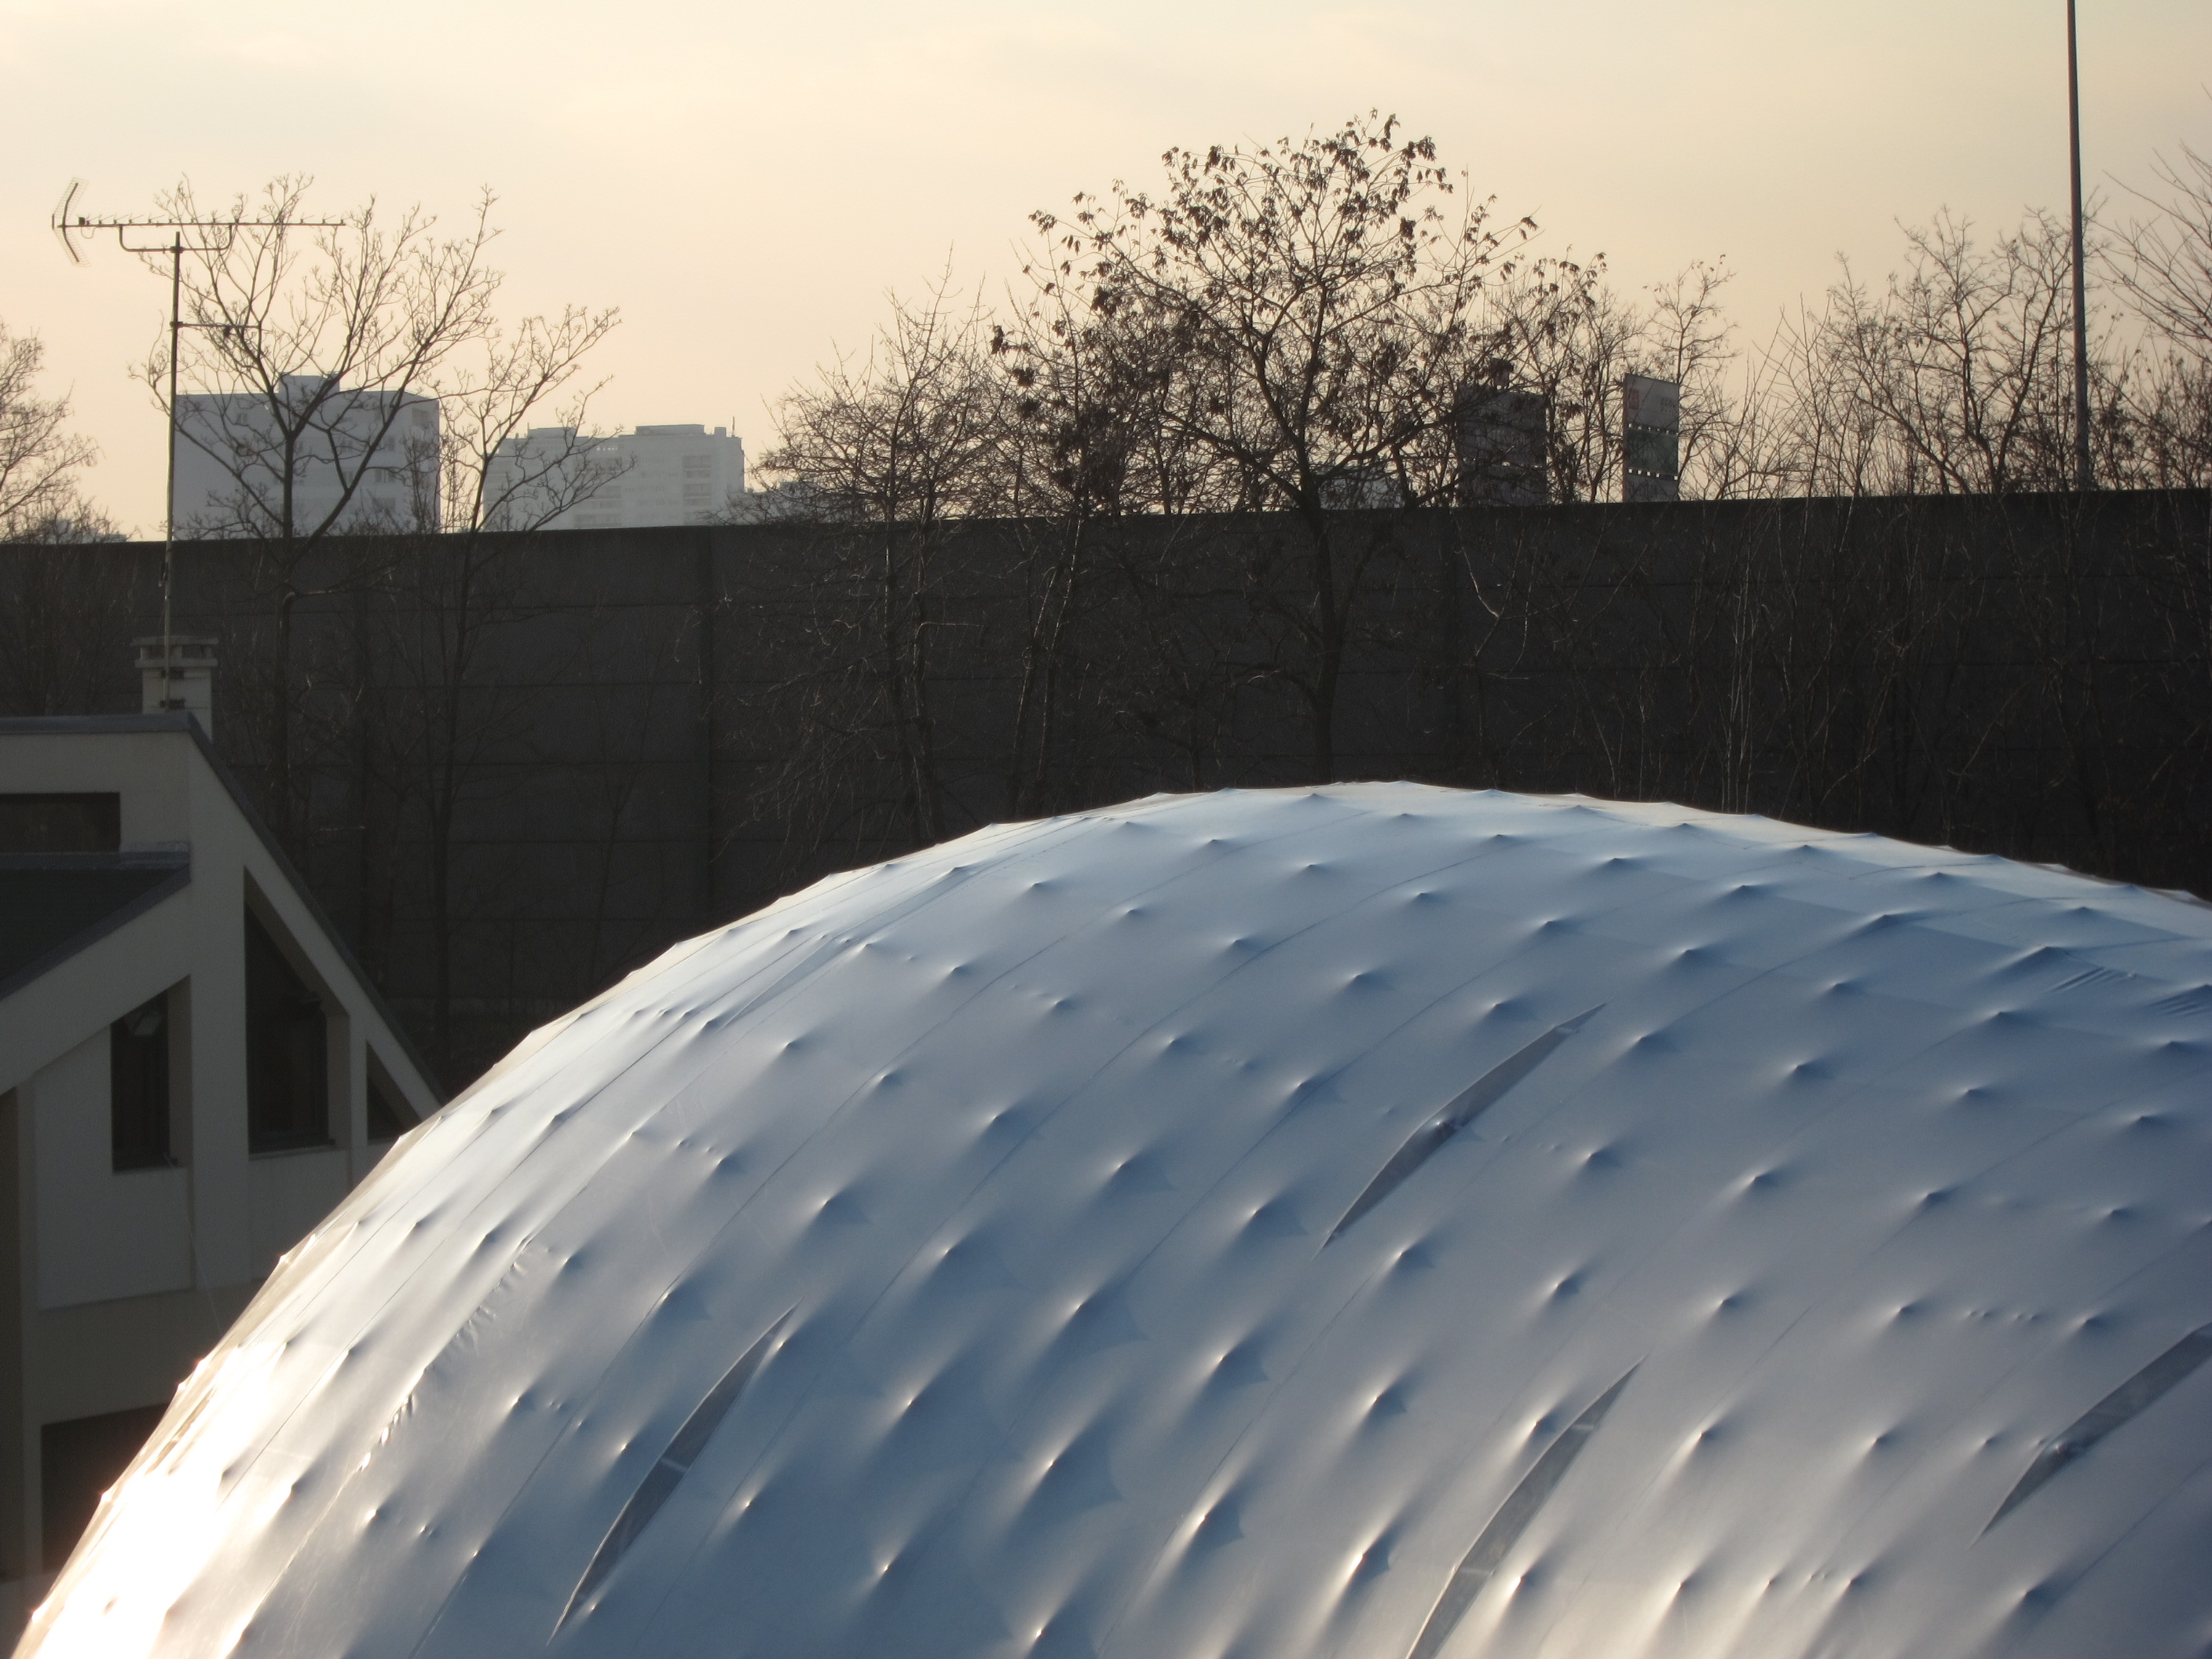
\includegraphics[width=\tmpwidth]{gs_ext}}
		\intersectnode{PPtl |- CAtl}{Pt}
		\Photo[
			node=Pt,
			anchor=north west,
			xshift=0mm,
			gopt={width=\tmpwidth},
			]{gs_ext.jpg}%
		\savenodes{A}
		\intersectnode{CAtl |- Abr}{Pt}
		\PhotoCaptionRef[
			hrefnode=Atl,
			node=Atr,
			anchor=south east,
			yshift=\PhotoRefSkip,
			phantom=true,
			]{figure}{}{Exterior view}{fig:gs_ext}
		\intersectnode{CAtl |- Abr}{Pt}
		\PhotoTextBox[
			node=CAbl,
			anchor=south west,
			% yshift=-\PhotoBigSkip,
			border=false,
			% width=4cm-\PhotoSkip,
			]{%
				\figurecaption[The connections mark the fabric suggesting the interior grid structure. This texture enriches the perception of the building viewed from the outside and creates effects with the light reflections.]{fig:gs_ext}
			}
	}
	\doubleblankpage[l]{%
		\hbox{}\thispagestyle{empty}
		\PhotoSpread[
			node=CAtl,
			anchor=north west,
			gopt={height=\textheight}
		]{gs_int.jpg}
		\AddToShipoutPictureBG*{
			\PhotoCaptionRef[
				hrefnode=TL,
				node=BL, 
				anchor=north west,
				yshift=-\PhotoRefSkip,
				phantom=true,
			]{figure}{}{Interior view}{fig:gs_int}}
	}{%
		\hbox{}\thispagestyle{empty}
		\AddToShipoutPictureBG*{
		\PhotoTextBox[
			node=BR,
			anchor=south west,
			xshift=\PhotoBigSkip,
			border=false,
			]{%
				\figurecaption[The grid pattern highlights the lightness of the structure and gives its tempo to the internal space. Lines converge to the altar, the heart of the liturgical area where the mass is offered on.]{fig:gs_int}
			}
	}}
}

\subsection{Daylight}
The gridshell is covered by a PVC membrane, which is opaque. How to introduce daylight into the interior was a major subject of reflection. The simplest way found was to use transparent membrane placed occasionally on the membrane. A small amount of light was required in the interior to create a contemplative atmosphere. The lights would in consequence glow and would be seen as luminous insertions in the vault, like stars in the celestial vault or the apse of some Romanesque churches. The stars were patterned on the joints of the PVC membrane. The almond shape came from simplification of the cutting into the panels either side of the joints and to avoid stress concentrations around cuts in the membrane. This shape, known as Mandela, is frequently used in Marian religious imagery. The distribution of the transparent insertions is quite uniform but gets denser above the pinnacle.

\enlargethispage{-4.5cm}
\AddToShipoutPictureBG*{% 
	\setlength{\tmpwidth}{\textwidth+\ContentInnerMargin+\BleedInnerMargin+\ContentBindingOffset}
	\settoheight{\tmpheight}{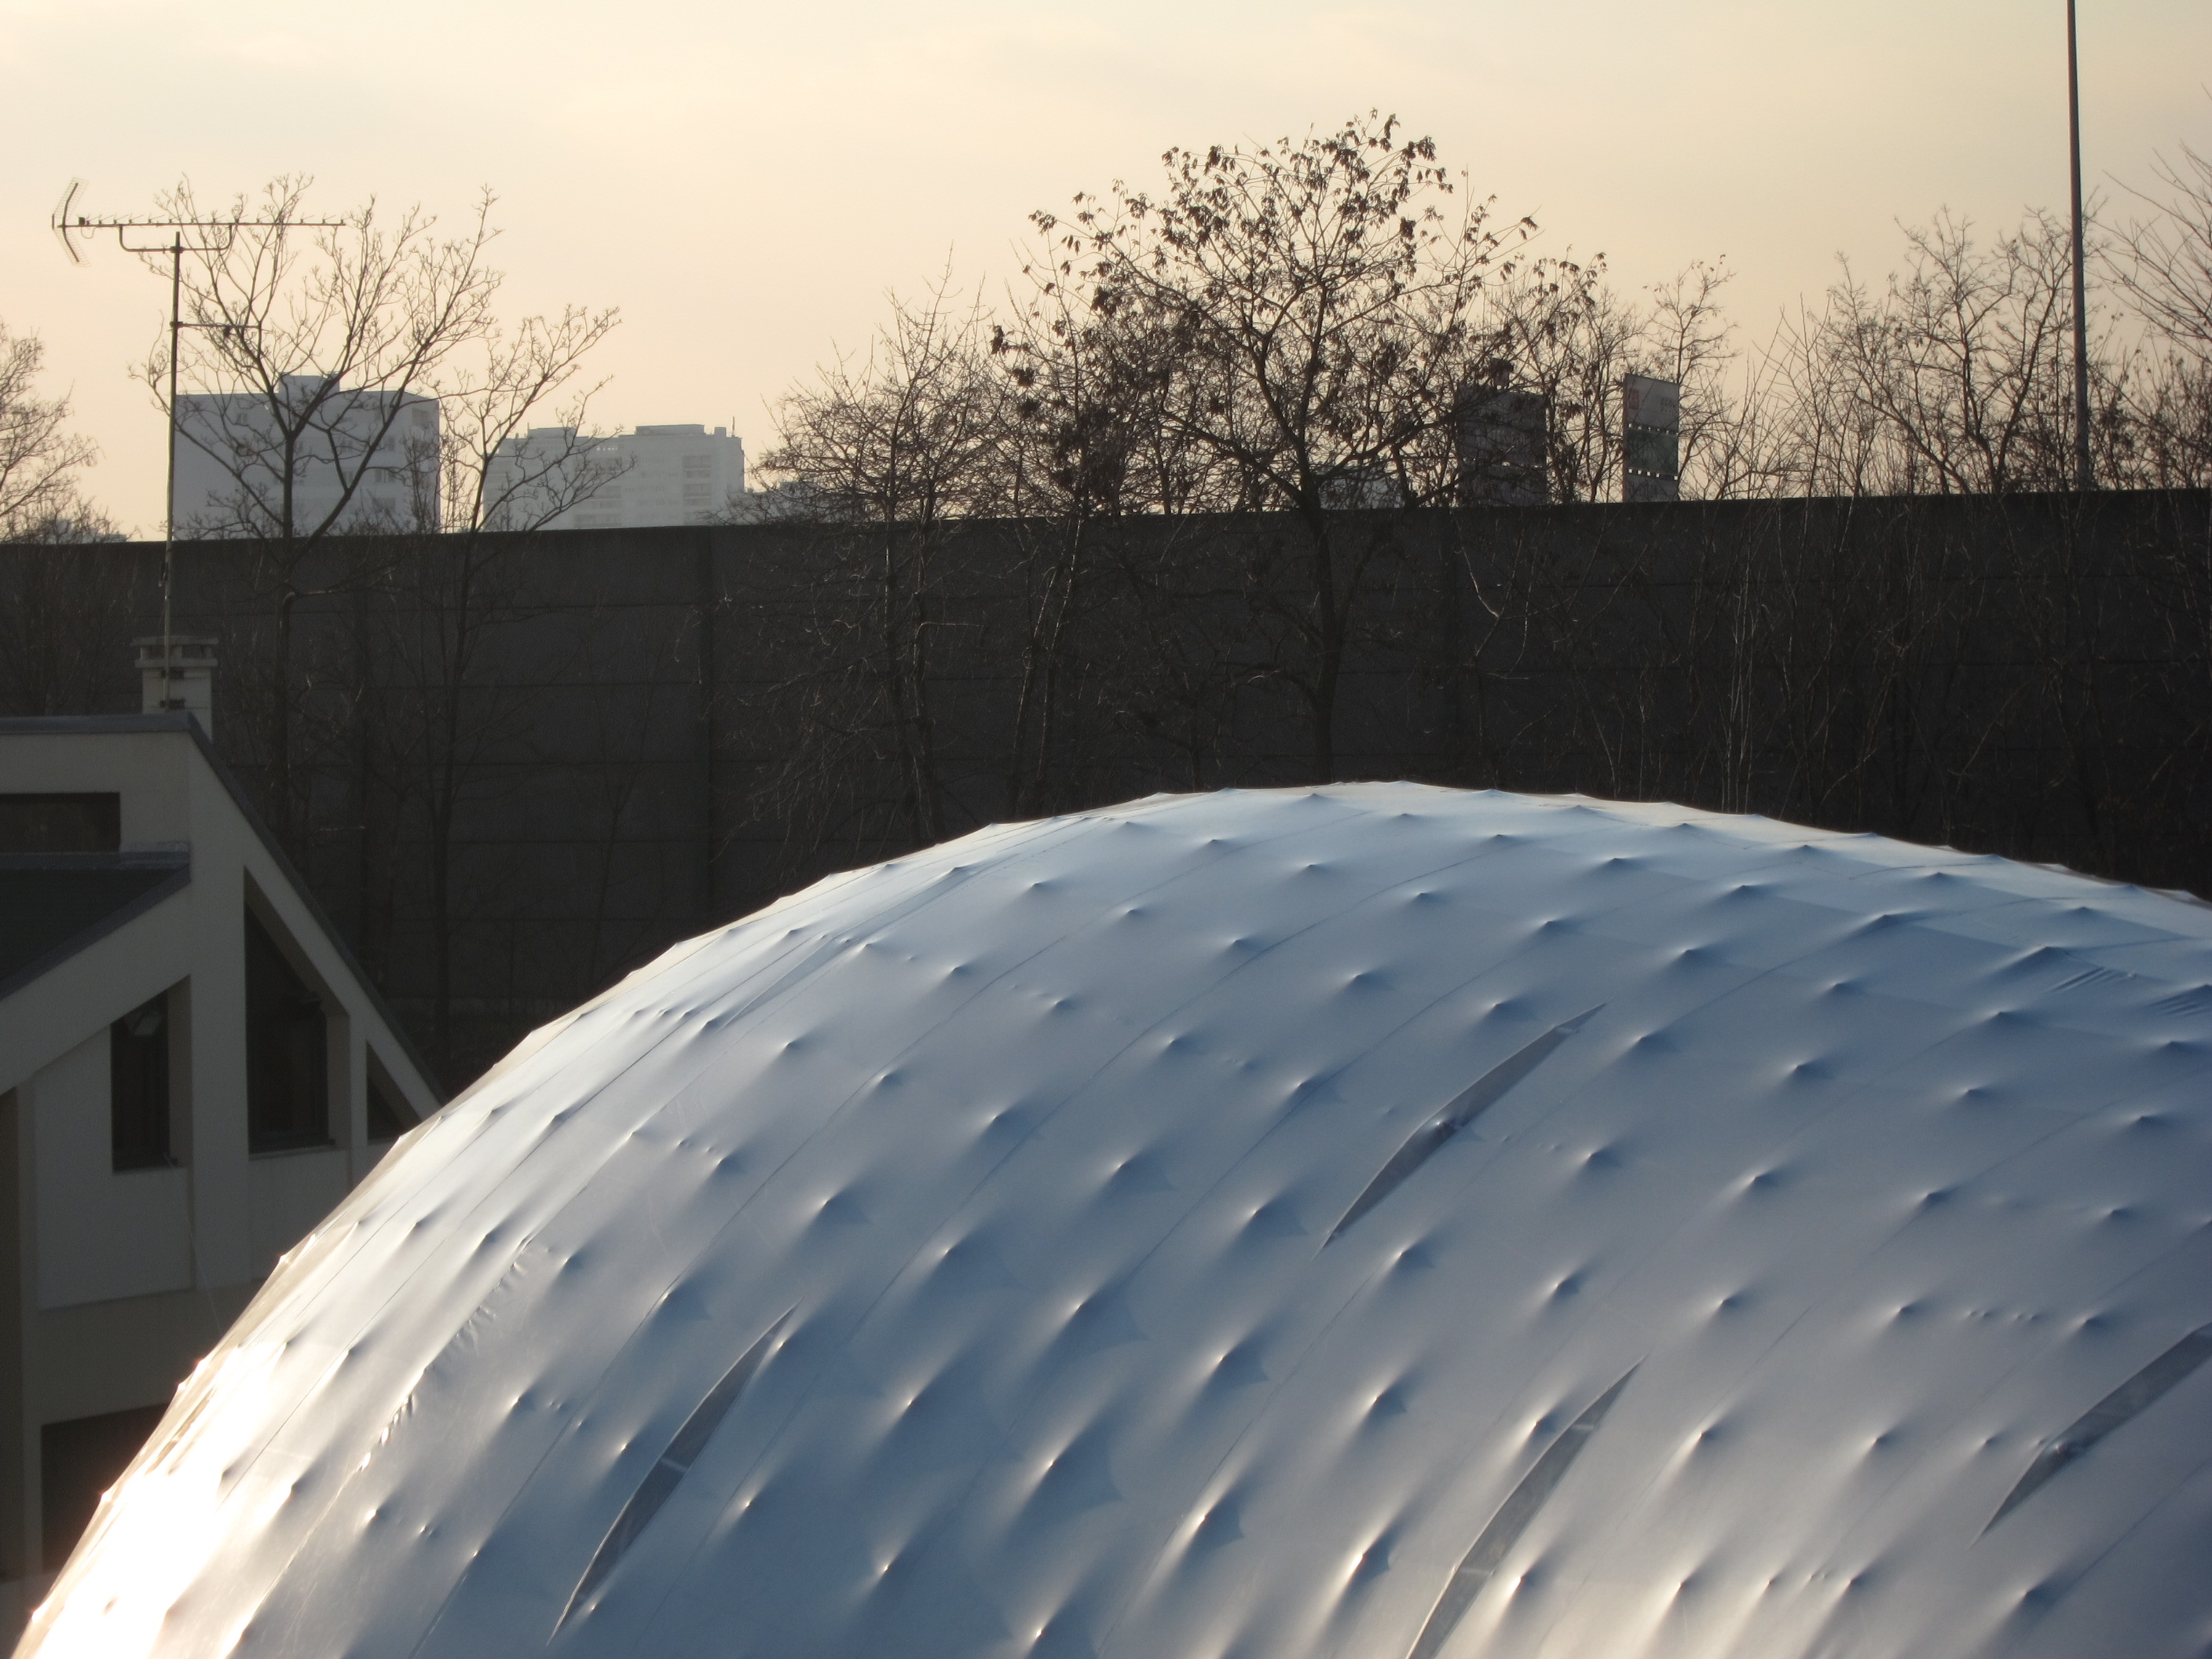
\includegraphics[height=4cm]{gs_ext}}
	\intersectnode{PPtl |- CAtl}{Pt}
	\Photo[
		node=CAbl,
		anchor=south west,
		gopt={height=4cm},
		]{door_ext.jpg}%
	\savenodes{A}
	\Photo[
		node=Atr,
		anchor=north west,
		xshift=\PhotoSkip,
		gopt={height=4cm},
		]{door_int.jpg}%
	\savenodes{B}
	\PhotoCaptionRef[
			node=Atl,
			anchor=north west,
			phantom=true;
			]{figure}{}{Steel doors}{fig:door}
		\PhotoCaptionRef[
			hrefnode=Atl,
			node=Atl,
			anchor=south west,
			yshift=\PhotoRefSkip,
			]{subfigure}{}{Interior view}{fig:door_int}
		\PhotoCaptionRef[
			hrefnode=Btl,
			node=Btl,
			anchor=south west,
			yshift=\PhotoRefSkip,
			]{subfigure}{}{Exterior view}{fig:door_ext}
	\PhotoTextBox[
		node=Bbr,
		anchor=south west,
		xshift=\PhotoSkip,
		border=false,
		width=4cm-\PhotoSkip,
		]{%
			\figurecaption[Two steel doors allow the entrance inside the building.]{fig:door}\par\bigskip
			\figurecaption{fig:door_int}\par
			\figurecaption{fig:door_ext}
		}
}

\subsection{Technical description}
% ------------------------------------------


\blankpage{%
	\thispagestyle{empty}
	\hbox{}
	\AddToShipoutPictureBG*{% 
		\def\tmpwidth{(\textwidth+\ContentOuterMargin+\BleedOuterMargin-\PhotoSkip)/2}
		\Photo[
			node=CAtl,
			anchor=north west,
			xshift=0mm,
			gopt={width=\tmpwidth},
			]{swivel.jpg}%
		\savenodes{A}
		\Photo[
			node=Atr,
			anchor=north west,
			xshift=\PhotoSkip,
			gopt={width=\tmpwidth},
			]{sleeve.jpg}%
		\savenodes{B}
		\Photo[
			node=Abl,
			anchor=north west,
			yshift=-\PhotoBigSkip,
			gopt={width=\tmpwidth},
			]{anchorage.jpg}%%
		\savenodes{C}
		\Photo[
			node=Bbl,
			anchor=north west,
			yshift=-\PhotoBigSkip,
			gopt={width=\tmpwidth},
			]{edge.jpg}%
		\savenodes{D}
		%%
		\PhotoCaptionRef[
			node=Atl,
			anchor=south west,
			yshift=-\PhotoSkip,
			phantom=true,
			]{figure}{}{Key elements of the structural system}{fig:parts}
		\PhotoCaptionRef[
			hrefnode=Atl,
			node=Atl, 
			anchor=south west, 
			yshift=\PhotoRefSkip,
			]{subfigure}{}{Swivel coupler}{fig:swivel}
		\PhotoCaptionRef[
			hrefnode=Btl,
			node=Btl, 
			anchor=south west, 
			yshift=\PhotoRefSkip,
			]{subfigure}{}{Sleeve system}{fig:sleeve}
		\PhotoCaptionRef[
			hrefnode=Ctl,
			node=Cbl, 
			anchor=north west, 
			yshift=-\PhotoRefSkip,
			]{subfigure}{}{Ground anchorage}{fig:anchorage}
		\PhotoCaptionRef[
			hrefnode=Dtl,
			node=Dbl, 
			anchor=north west, 
			yshift=-\PhotoRefSkip,
			]{subfigure}{}{Lacing rod}{fig:edge}
		\PhotoTextBox[
			node=CAbl,
			anchor=south west,
			width=10cm,
			border=false,
			]{%
				\figurecaption{fig:parts}\par
				\figurecaption{fig:swivel}\par
				\figurecaption{fig:sleeve}\par
				\figurecaption{fig:anchorage}\par
				\figurecaption{fig:edge}
			}
	}
}

The gridshell structure is made of long glass fibre tubes (\O 42~mm) fastened together with scaffold swivel couplers (see, \cref{fig:swivel}). The structural members of the grid, all of different lengths, are built  from one, two or three composite tubes connected with steel sleeves (see \cref{fig:sleeve}). The length of the tubes is limited to 12~m to enable transportation through standard trucks. The tubes are organized in three layers. During assembly, the first two layers are first placed perpendicular to one another on the ground. They form the \emph{quadrangular primary grid}. The distance between the tubes of these two layers is constant, resulting in a regular grid. This primary grid is elastically deformed to obtain the final shape. The third layer of tubes acts as bracing. It gives the structure a shell-like behavior. The tubes are fixed to the primary grid once the shape has been obtained.

The structure is anchored to a concrete strip footing with a special anchorage system, which ensures transfer of loads from the composite structure to the ground (see \cref{fig:anchorage}). A similar system enables fixation of the structure to the doors (see \cref{fig:door_int}).

A PVC coated fabric (see \cref{fig:gs_ext}), tailor-made for the purpose, covers the structure. The transparent portion of the structure allows daylight inside the gridshell. The fabric is stretched on the peripheral edge of a dedicated beam with a double-lacing system (halyard and strap, see \cref{fig:edge}). At the ground level, the lacing edge of the beam is made of a bent composite rod nailed to the concrete slab. At the grid–door junction, a steel arch is welded to the doorframe (see \cref{fig:door_ext}). The PVC fabric is waterproof and, since it is a continuous membrane, has no joints except at the perimeter. At the perimeter, a continuous strip of membrane is prefixed to the internal surface of the membrane and fixed to the ground slab. At the doors, a flexible strip of the membrane is riveted to the doorframe.

\blankpage{
	\hbox{}\thispagestyle{empty}
	\AddToShipoutPictureBG*{
		\SBox[%
			node=CAc,
			anchor=center,
			]{%
				\begin{tabular}{@{}lllrr@{}}
					\toprule
					Category	 & Item 						& Unit 						& Quantity\\
					\midrule
					Public  	& seating  						& p							& 360 \\
								& standing 						& p							& 500 \\
					\midrule
				%	\addlinespace[0.5cm]
					Dimensions  &  length						& m 						& 29	\\
								&  width 						& m							& 17	\\
								&  height 						& m							& 7	\\
								& contour 	 					& lm						& 75\\
								& area							& m\textsuperscript{2}		& 350\\
								&  volume						& m\textsuperscript{3}		& 1600 \\
					\midrule
				%	\addlinespace[0.5cm]
					Gridshell   &  tubes (x176)					& lm						& 1775 \\
								&  connections					& 							& 1130 \\
								&  sleeves						& 							& 125 \\
								& anchorages 					& 							& 127 \\
								& \quad \emph{ground (single)} 	& 							& 77 \\
								& \quad \emph{ground (double)} 	& 							& 16 \\
								& \quad \emph{door (single)} 	& 							& 18 \\
								& weight  						& kg/m\textsuperscript{2} 	& 5 \\
					\midrule
				%	\addlinespace[0.5cm]
					Fabric   	& opaque						& m\textsuperscript{2}	 	& 530 \\
								& transparent					& m\textsuperscript{2}		& 12 \\
								& lacing rod					& lm 				 		& 67 \\
								& weight						& kg/m\textsuperscript{2}	& 1 \\
					\bottomrule
				\end{tabular}
			}
		\PhotoCaptionRef[
			node=CAtl, 
			anchor=north west, 
			% yshift=-\PhotoRefSkip,
			phantom=true,
			]{table}{}{Key figures}{tab:kfigures}
		\PhotoTextBox[
			node=CAbl,
			anchor=south west,
			width=0.6\textwidth,
			border=false,
			]{\tablecaption{tab:kfigures}}
	}
}


\blankpage{
	\thispagestyle{empty}
	\hbox{}
	\AddToShipoutPictureBG*{% 
		\def\tmpwidth{\textwidth+\ContentOuterMargin+\BleedOuterMargin}
		\intersectnode{PPtl |- CAtl}{Pt}
		\Photo[
			node=Pt,
			anchor=north west,
			xshift=0mm,
			gopt={width=\PaperWidth},
			]{plan_view2}%
		\savenodes{A}
		\PhotoCaptionRef[
			node=Atl,
			anchor=south west,
			yshift=-\PhotoSkip,
			phantom=true,
			]{figure}{}{Top view of the building}{fig:plan_view}
		\PhotoTextBox[
			node=CAbl,
			anchor=south west,
			width=8cm,
			border=false,
			]{%
				\figurecaption[The interior space is composed of a choir (1), a place of assembly (2) and a narthex (3). The main entrance overlook the parvis (4). The shell spans about 29~m in the longitudinal direction and about 17~m in the transversal direction. The covered area is about 350~m\textsuperscript{2}. The space can accommodate 360 seating people or 500 standing people.]{fig:plan_view}\par
			}
	}

	\doubleblankpage{%
		\hbox{}\thispagestyle{empty}
		\intersectnode{PPtl |- CAbl}{Pt}
		\PhotoSpread[
			node=Pt,
			anchor=south west,
			yshift=-5cm,
			% lpcode={\thispagestyle{empty}},
			% rpcode={\thispagestyle{fancy}},
			gopt={width=2\PaperWidth}
		]{section_view2}
		\AddToShipoutPictureBG*{
			\PhotoCaptionRef[
				hrefnode=TL,
				node=BL, 
				anchor=north west,
				yshift=-\PhotoRefSkip,
				phantom=true,
			]{figure}{}{Transversal section of the building}{fig:sec}
			\PhotoTextBox[
				node=CAtl,
				anchor=north west,
				% xshift=\PhotoBigSkip,
				border=false,
			]{%
				\figurecaption[Observe how the grid gets denser at the choir. Two doors give access to the building. The height at the pinnacle is about 7~m.]{fig:sec}
			}
		}
	}{%
		\hbox{}\thispagestyle{empty}
		\AddToShipoutPictureBG*{
		\Photo[
			node=CAtr,
			anchor=north east,
			xshift=0mm,
			gopt={width=5cm},
			]{section_view_detail}%
		\savenodes{A}	
	}}
}



% \doubleblankpage[l]{
% 	\thispagestyle{empty}
% 	\hbox{}
% 	\AddToShipoutPictureBG*{% 
% 		\setlength{\tmpwidth}{\textwidth+\ContentInnerMargin+\BleedInnerMargin+\ContentBindingOffset}
% 		\intersectnode{PPtl |- CAbl}{Pt}
% 		\Photo[
% 			node=Pt,
% 			anchor=south west,
% 			% yshift=-\PhotoBigSkip,
% 			gopt={width=\tmpwidth},
% 			]{section_view}%
% 		\savenodes{B}
% 		\PhotoCaptionRef[
% 			node=Atl,
% 			anchor=south west,
% 			yshift=-\PhotoSkip,
% 			phantom=true,
% 			]{figure}{}{Transversal section of the building}{fig:sec}
% 		\PhotoTextBox[
% 			node=CAtl,
% 			anchor=north west,
% 			% width=10cm,
% 			border=false,
% 			]{%
% 				\figurecaption[Observe how the grid gets denser at the choir. Two doors give access to the building. The height at the pinnacle is about 7~m.]{fig:sec}
% 			}
% 	}
% }{%
% 	\thispagestyle{empty}
% 	\hbox{}
% }

% \begin{figure}[p]
% 	\captionsetup[subfloat]{captionskip=20pt}
%      	\centering
% 	\begin{fullpage}
% 		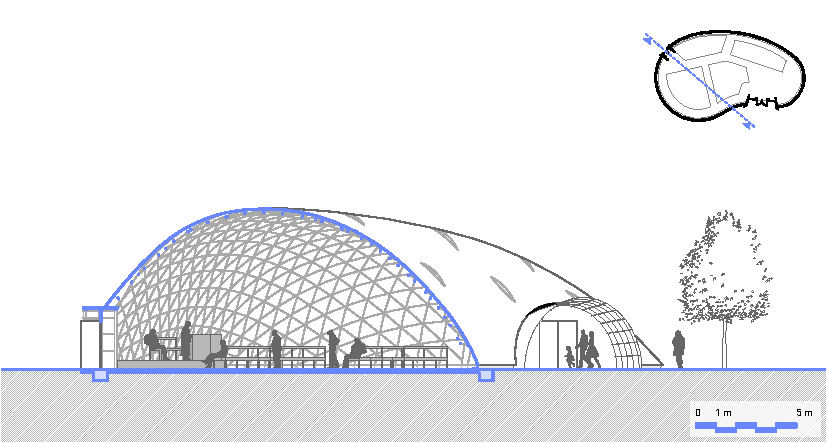
\includegraphics[width=\textwidth]{section_view}
% 		\caption[Transversal section of the building]{Transversal section of the building. Observe how the grid gets denser at the choir. Two doors give access to the building. The height at the pinnacle is about 7~m.}
% 		\label{fig:sec}
% 		%
% 		\vspace{1.5cm}
% 		%
% 		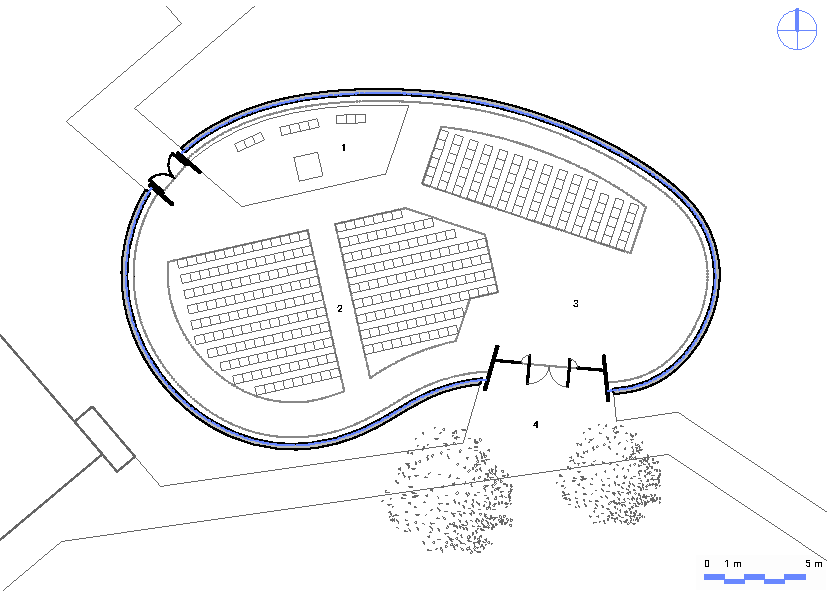
\includegraphics[width=\textwidth]{plan_view}
% 		\caption[Top view of the building]{Top view of the building. The interior space is composed of a choir (1), a place of assembly (2) and a narthex (3). The main entrance overlook the parvis (4). The shell spans about 29~m in the longitudinal direction and about 17~m in the transversal direction. The covered area is about 350~m\textsuperscript{2}. The space can accommodate 360 seating people or 500 standing people.}
% 		\label{fig:plan_view}
% 	\end{fullpage}
% \end{figure}


\pagebreak
\section{Construction process}\label{sec=construction_process}
% ====================

\subsection{Assembly of the grid}
The first two directions of tubes were assembled perpendicularly on the ground with the swivel couplers (see \cref{fig:swivel}) to form the \emph{primary} grid. The resulting grid covered about 600~m\textsuperscript{2} (see \cref{fig:cp_1}). At each intersection, the tubes were fastened together with a coupler, installed manually by the volunteers. They were asked not to tighten the bolts but just to engage the collars in order to prevent potential damages from the collar over the tube. Once the assembly of the primary grid was complet, the swivel couplers were tightened with a torque wrench to the optimal torque specified by the laboratoire Navier (F. Tayeb, J-F. Caron, L. du Peloux). The whole stage took two full days. Note that because the anchorages sticked out from the slab, it was decided not to assemble the grid on the concrete slab to ensure that the grid would be able to slide freely on the ground and not get clung in the anchorages during the erection stage.

\subsection{Deformation of the grid}
The next stage consisted in lifting the grid simultaneously with two mobile cranes (35t). Once lifted up, the grid took nearly its final form (see \cref{fig:cp_2}). The structure was slowly moved above the slab until tube endings faced at best their respective anchor points. Then, tube after tube, the workers pined the grid to the ground anchorages (see \cref{fig:cp_3}). This stage is tricky, especially at the beginning because only few tubes are connected to the ground. If the grid moves it can easily break these few tubes. The action of pinning a tube is done with a single bolt. The end of each composite tube is equipped with a rotating steel clevis. Similarly, each ground anchorage is composed of a steel plate fixed to the concrete slab and a rotating clevis. To pin a tube to an anchorage, their clevis are aligned one to each other and a pin is positioned in their central hole (see \cref{fig:anchorage}). When all the tubes were pinned to their anchorage, the grid was stable and secured and the cranes were removed (see \cref{fig:cp_4}). This stage lasted one full day.

\setlength{\tmpheight}{(\textheight-2\PhotoBigSkip)/3}
\intersectnode{PPtr |- CAtr}{Pt}
\PhotoSpread[
	node=Pt,
	anchor=north west,
	xshift=-2\PhotoBigSkip,
	gopt={height=\tmpheight},
	rpcode={\savenodes{AA}},
	]{erec_1a.jpg}%

\afterpage{
	\thispagestyle{empty}
	\hbox{\vspace{\textheight}}
	% \hbox{\vspace*{1cm}}
	\AddToShipoutPictureBG*{% 
		\intersectnode{PPtl |- CAtl}{Pt}
		% \def\tmpheight{(\textheight-2\PhotoBigSkip)/3}
		\Photo[
			node=AAtr,
			anchor=north west,
			xshift=\PhotoSkip,
			gopt={height=\tmpheight},
			]{erec_1b.jpg}%	
			\savenodes{AB}
		\intersectnode{CAtl |- AAtr}{Pt}
		\PhotoCaptionRef[
			hrefnode=CAtl,
			node=CAtl, 
			anchor=south west, 
			yshift=\PhotoRefSkip,
			phantom=true,
			]{figure}{}{Assembly of the grid}{fig:erec_1}
		\PhotoCaptionRef[
			hrefnode=CAtl,
			node=CAtl, 
			anchor=south west, 
			yshift=\PhotoRefSkip,
		]{subfigure}{}{GFRP tubes with swivel couplers}{fig:erec_1a}
		\PhotoCaptionRef[
			hrefnode=ABtl,
			node=ABtl, 
			anchor=south west, 
			yshift=\PhotoRefSkip,
			]{subfigure}{}{Primary grid}{fig:erec_1b}
	}
	\PhotoSpread[
		node=ABtr,
		anchor=north west,
		xshift=\PhotoWidth+\PhotoBigSkip,
		gopt={height=\tmpheight},
		]{erec_1c.jpg}%
	% \savenodes{AC}
	\AddToShipoutPictureBG*{%
		\PhotoCaptionRef[
			hrefnode=PStl,
			node=PStl, 
			anchor=south west, 
			yshift=\PhotoRefSkip,
			]{subfigure}{}{Cranes ready to lift the grid}{fig:erec_1c}
		\intersectnode{PPtl |- AAbr}{Pt}
		\Photo[
			node=Pt,
			anchor=north west,
			% xshift=\PhotoSkip,
			yshift=-\PhotoBigSkip,
			gopt={height=\tmpheight},
			]{erec_2a.jpg}%	
			\savenodes{BA}
		\Photo[
			node=BAtr,
			anchor=north west,
			xshift=\PhotoSkip,
			% yshift=-\PhotoBigSkip,
			gopt={height=\tmpheight},
			]{erec_2b.jpg}%	
			\savenodes{BB}
		\Photo[
			node=BAbl,
			anchor=north west,
			xshift=2\PhotoBigSkip,
			yshift=-\PhotoBigSkip,
			gopt={height=\tmpheight},
			]{erec_3a.jpg}%
		\savenodes{BC}
		%%
		\intersectnode{CAtl |- BBtr}{Pt}
		\PhotoCaptionRef[
			hrefnode=Pt,
			node=Pt, 
			anchor=south west, 
			yshift=\PhotoRefSkip,
			phantom=true,
			]{figure}{}{Deformation of the grid}{fig:erec_2}
		\PhotoCaptionRef[
			hrefnode=Pt,
			node=Pt, 
			anchor=south west, 
			yshift=\PhotoRefSkip,
		]{subfigure}{}{GFRP tubes with swivel couplers}{fig:erec_2a}
		\PhotoCaptionRef[
			hrefnode=BBtl,
			node=BBtl, 
			anchor=south west, 
			yshift=\PhotoRefSkip,
			]{subfigure}{}{Primary grid}{fig:erec_2b}
		\intersectnode{CAtl |- BCtr}{Pt}
		\PhotoCaptionRef[
			hrefnode=Pt,
			node=Pt, 
			anchor=south west, 
			yshift=\PhotoRefSkip,
			]{subfigure}{}{Primary grid}{fig:erec_2c}
		\PhotoTextBox[
			node=BCbr,
			anchor=south west,
			xshift=\PhotoBigSkip,
			width=10cm,
			border=false,
			]{%
				\figurecaption{fig:erec_1}\par
				\figurecaption{fig:erec_1a}\par
				\figurecaption{fig:erec_1b}\par
				\figurecaption{fig:erec_1c}\par\medskip
				\figurecaption{fig:erec_2}\par
				\figurecaption{fig:erec_2a}\par
				\figurecaption{fig:erec_2b}\par
				\figurecaption{fig:erec_2c}
			}
	}
	%%
	\blankpage{%
		\thispagestyle{empty}
		\hbox{}
		\AddToShipoutPictureBG*{% 
			\intersectnode{PGtl |- AAbr}{Pt}
			\Photo[
				node=Pt,
				anchor=north west,
				xshift=2\PhotoBigSkip,
				yshift=-\PhotoBigSkip,
				gopt={height=\tmpheight},
				]{erec_4a.jpg}%
			\savenodes{DA}
			\Photo[
				node=DAtr,
				anchor=north west,
				xshift=\PhotoSkip,
				% yshift=-\PhotoBigSkip,
				gopt={height=\tmpheight},
				]{erec_4b.jpg}%
			\savenodes{DB}
			%%
			\intersectnode{PPtl |- DBbr}{Pt}
			\Photo[
				node=Pt,
				anchor=north west,
				% xshift=2\PhotoBigSkip,
				yshift=-\PhotoBigSkip,
				gopt={height=\tmpheight},
				]{erec_5a.jpg}%
			\savenodes{EA}
			\Photo[
				node=EAtr,
				anchor=north west,
				xshift=\PhotoSkip,
				% yshift=-\PhotoBigSkip,
				gopt={height=\tmpheight},
				]{erec_5b.jpg}%
			\savenodes{EB}
			\Photo[
				node=EBtr,
				anchor=north west,
				xshift=\PhotoSkip,
				% yshift=-\PhotoBigSkip,
				gopt={height=\tmpheight},
				]{erec_5c.jpg}%
			\savenodes{EC}
			%%%%
			\intersectnode{CAtl |- BBtr}{Pt}
			\PhotoCaptionRef[
				hrefnode=DAtl,
				node=DAtl, 
				anchor=south west, 
				yshift=\PhotoRefSkip,
				phantom=true,
				]{figure}{}{Deformation of the grid}{fig:erec_3}
			\PhotoCaptionRef[
				hrefnode=DAtl,
				node=DAtl, 
				anchor=south west, 
				yshift=\PhotoRefSkip,
			]{subfigure}{}{GFRP tubes with swivel couplers}{fig:erec_3a}
			\PhotoCaptionRef[
				hrefnode=DBtl,
				node=DBtl, 
				anchor=south west, 
				yshift=\PhotoRefSkip,
				]{subfigure}{}{Primary grid}{fig:erec_3b}
			%%%
			\intersectnode{DAtl |- EAtr}{Pt}
			\PhotoCaptionRef[
				hrefnode=Pt,
				node=Pt, 
				anchor=south west, 
				yshift=\PhotoRefSkip,
				phantom=true,
				]{figure}{}{Deformation of the grid}{fig:erec_4}
			\PhotoCaptionRef[
				hrefnode=Pt,
				node=Pt, 
				anchor=south west, 
				yshift=\PhotoRefSkip,
			]{subfigure}{}{GFRP tubes with swivel couplers}{fig:erec_4a}
			\PhotoCaptionRef[
				hrefnode=EBtl,
				node=EBtl, 
				anchor=south west, 
				yshift=\PhotoRefSkip,
				]{subfigure}{}{Primary grid}{fig:erec_4b}
			\PhotoCaptionRef[
				hrefnode=ECtl,
				node=ECtl, 
				anchor=south west, 
				yshift=\PhotoRefSkip,
				]{subfigure}{}{Primary grid}{fig:erec_4c}
			\PhotoTextBox[
				node=AAtr,
				anchor=north west,
				xshift=\PhotoBigSkip,
				width=10cm,
				border=false,
				]{%
					\figurecaption{fig:erec_3}\par
					\figurecaption{fig:erec_3a}\par
					\figurecaption{fig:erec_3b}\par\medskip
					\figurecaption{fig:erec_4}\par
					\figurecaption{fig:erec_4a}\par
					\figurecaption{fig:erec_4b}\par
					\figurecaption{fig:erec_4c}
				}
		}
	}
}

\subsection{Bracing of the grid}
Once the primary grid was deformed into the final shape, it was braced by a third direction of tubes called the \emph{triangulation}. The triangulation tubes split the quadrangular mesh of the primary grid into triangles (see \cref{fig:cp_5}). This work was tedious as it required working at height in aerial buckets. Tubes were hand-conveyed in the structure and attached to the tubes of the second layer with an additional swivel coupler. Each node of the structure would then be composed of two connections (see \cref{fig:swivel_dwg}). Once triangulated the structure behaves like a shell and its stiffness increases largely.




% \begin{figure}[p]
% 	%
%      	\centering
% 	\begin{fullpage}
% 		\subfloat[][Flat grid]{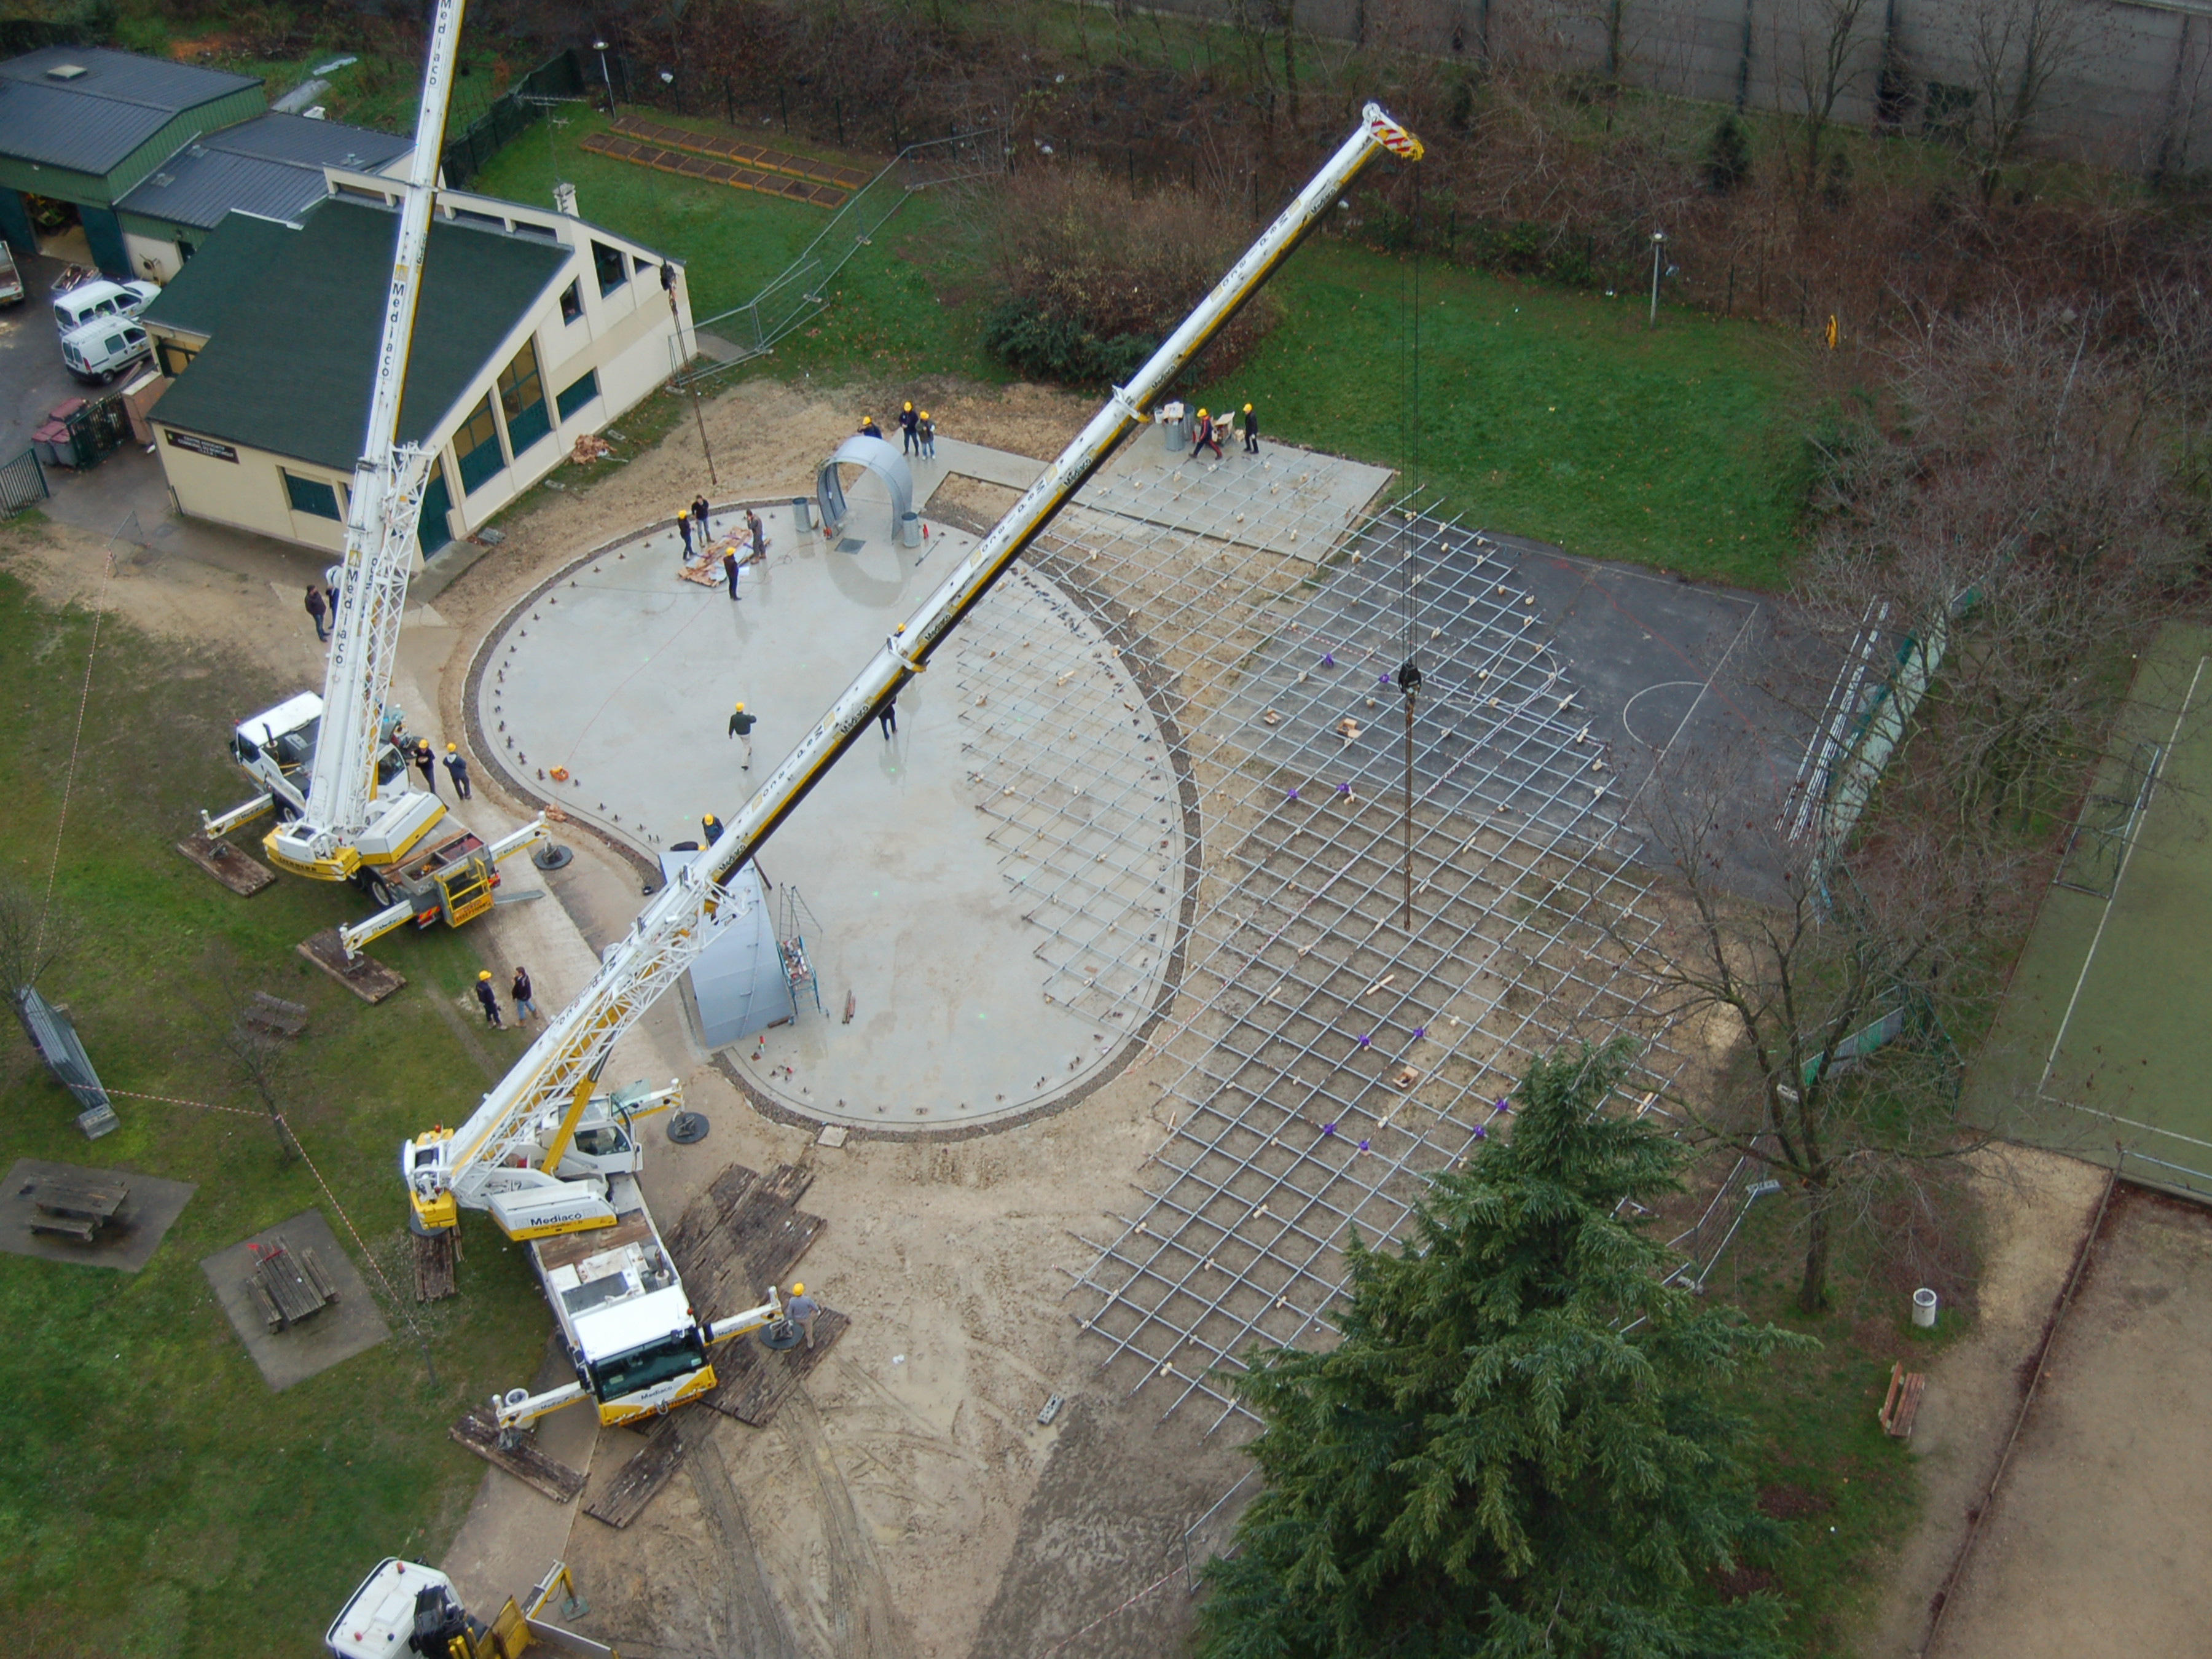
\includegraphics[width=0.48\textwidth]{cp_1.jpg}\label{fig:cp_1}}
% 		\hspace*{\fill}
% 		\subfloat[][Erection]{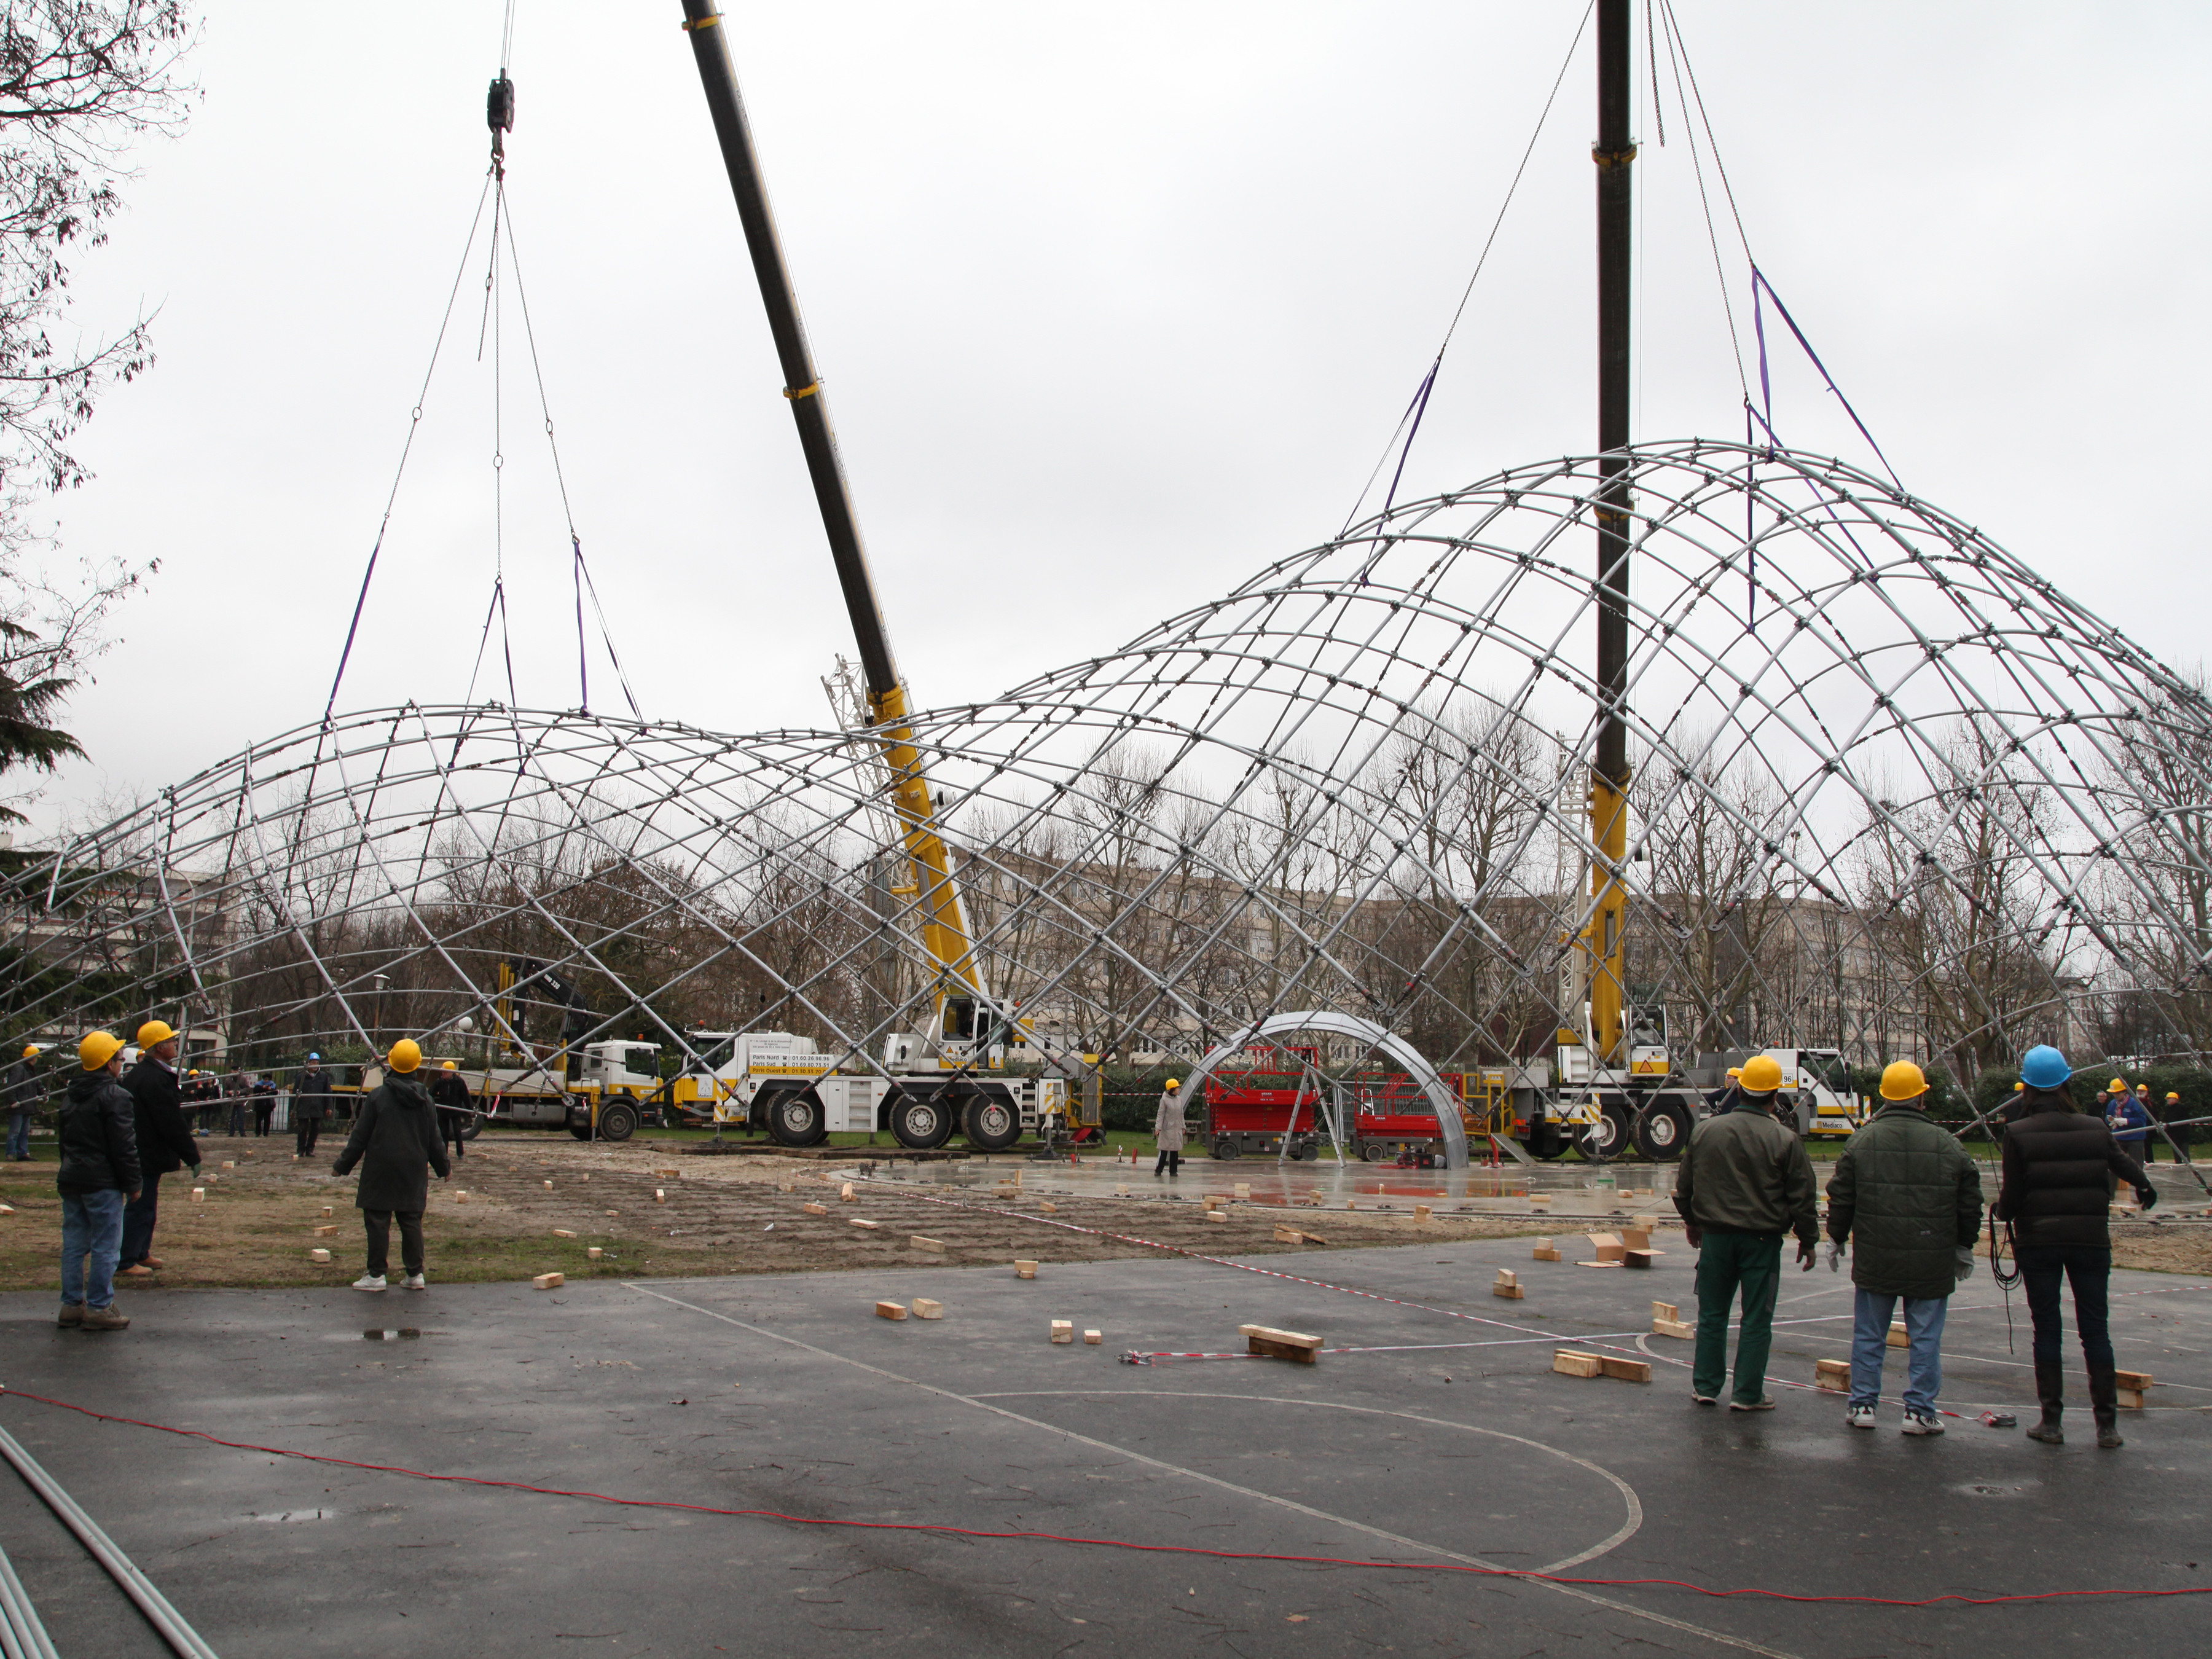
\includegraphics[width=0.48\textwidth]{cp_2.jpg}\label{fig:cp_2}} \\
% 		%
% 		\subfloat[][The grid is anchored]{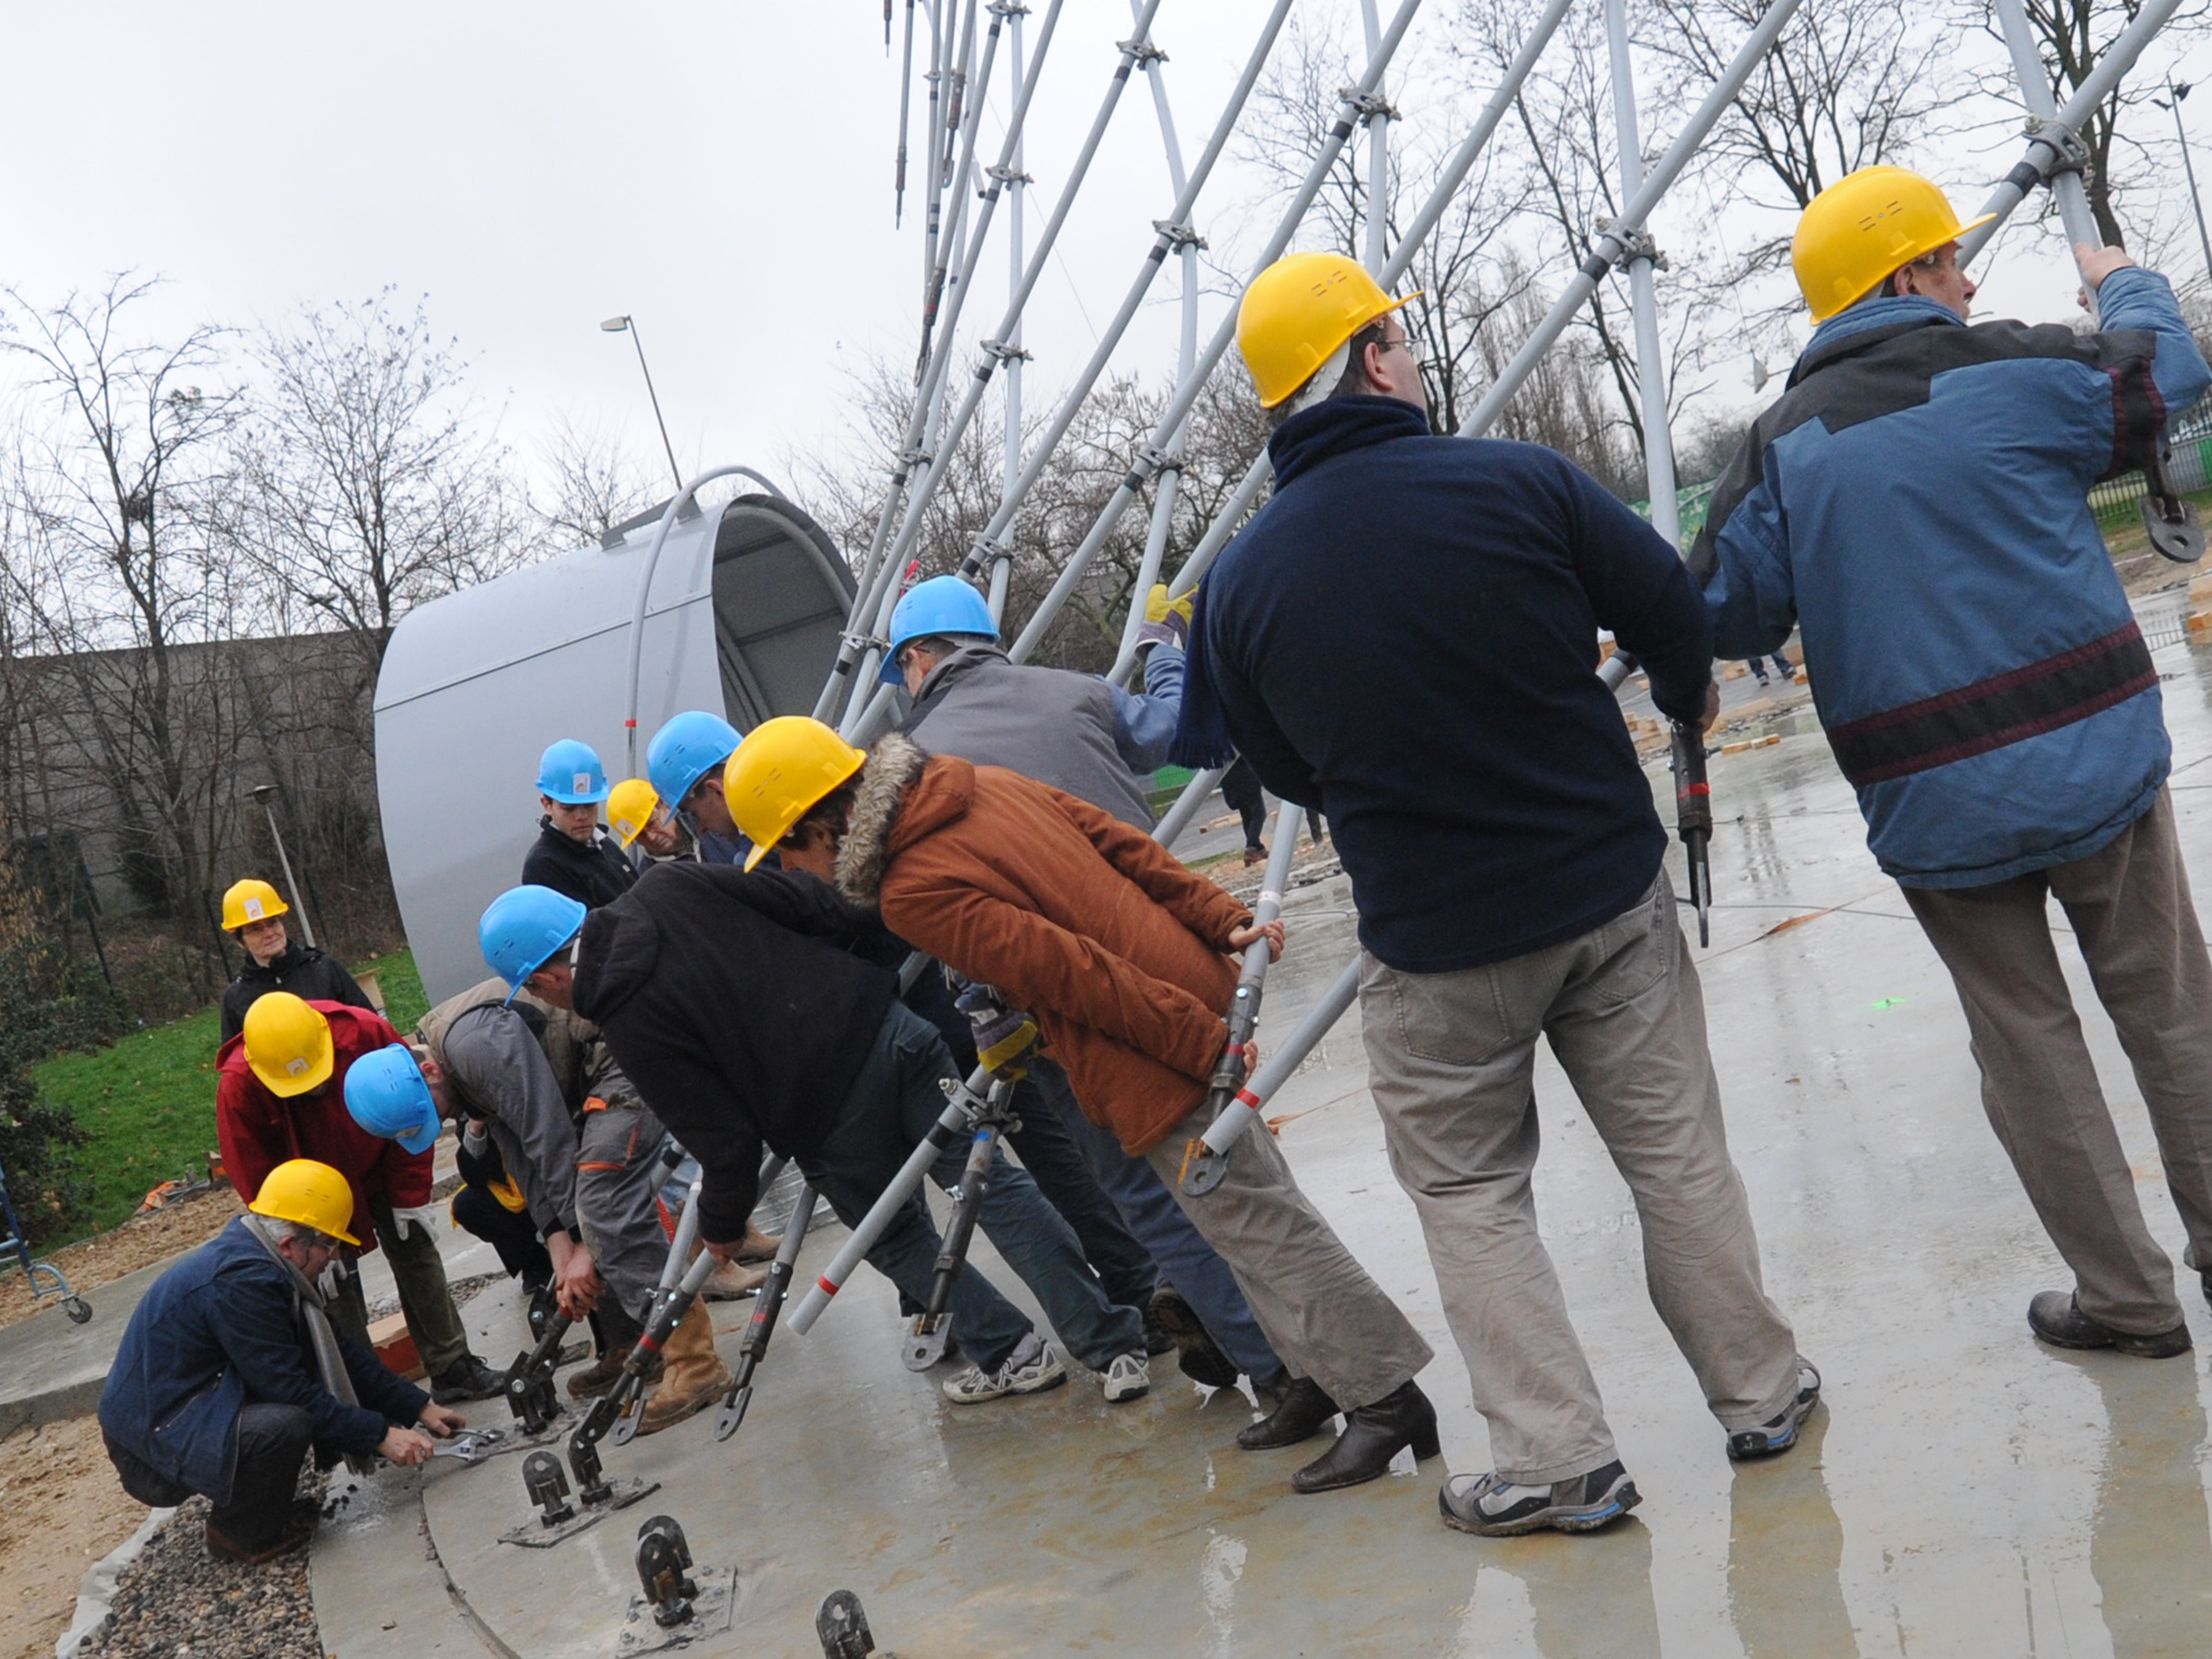
\includegraphics[width=0.48\textwidth]{cp_3.jpg}\label{fig:cp_3}}
% 		\hspace*{\fill}
% 		\subfloat[][Deformed grid]{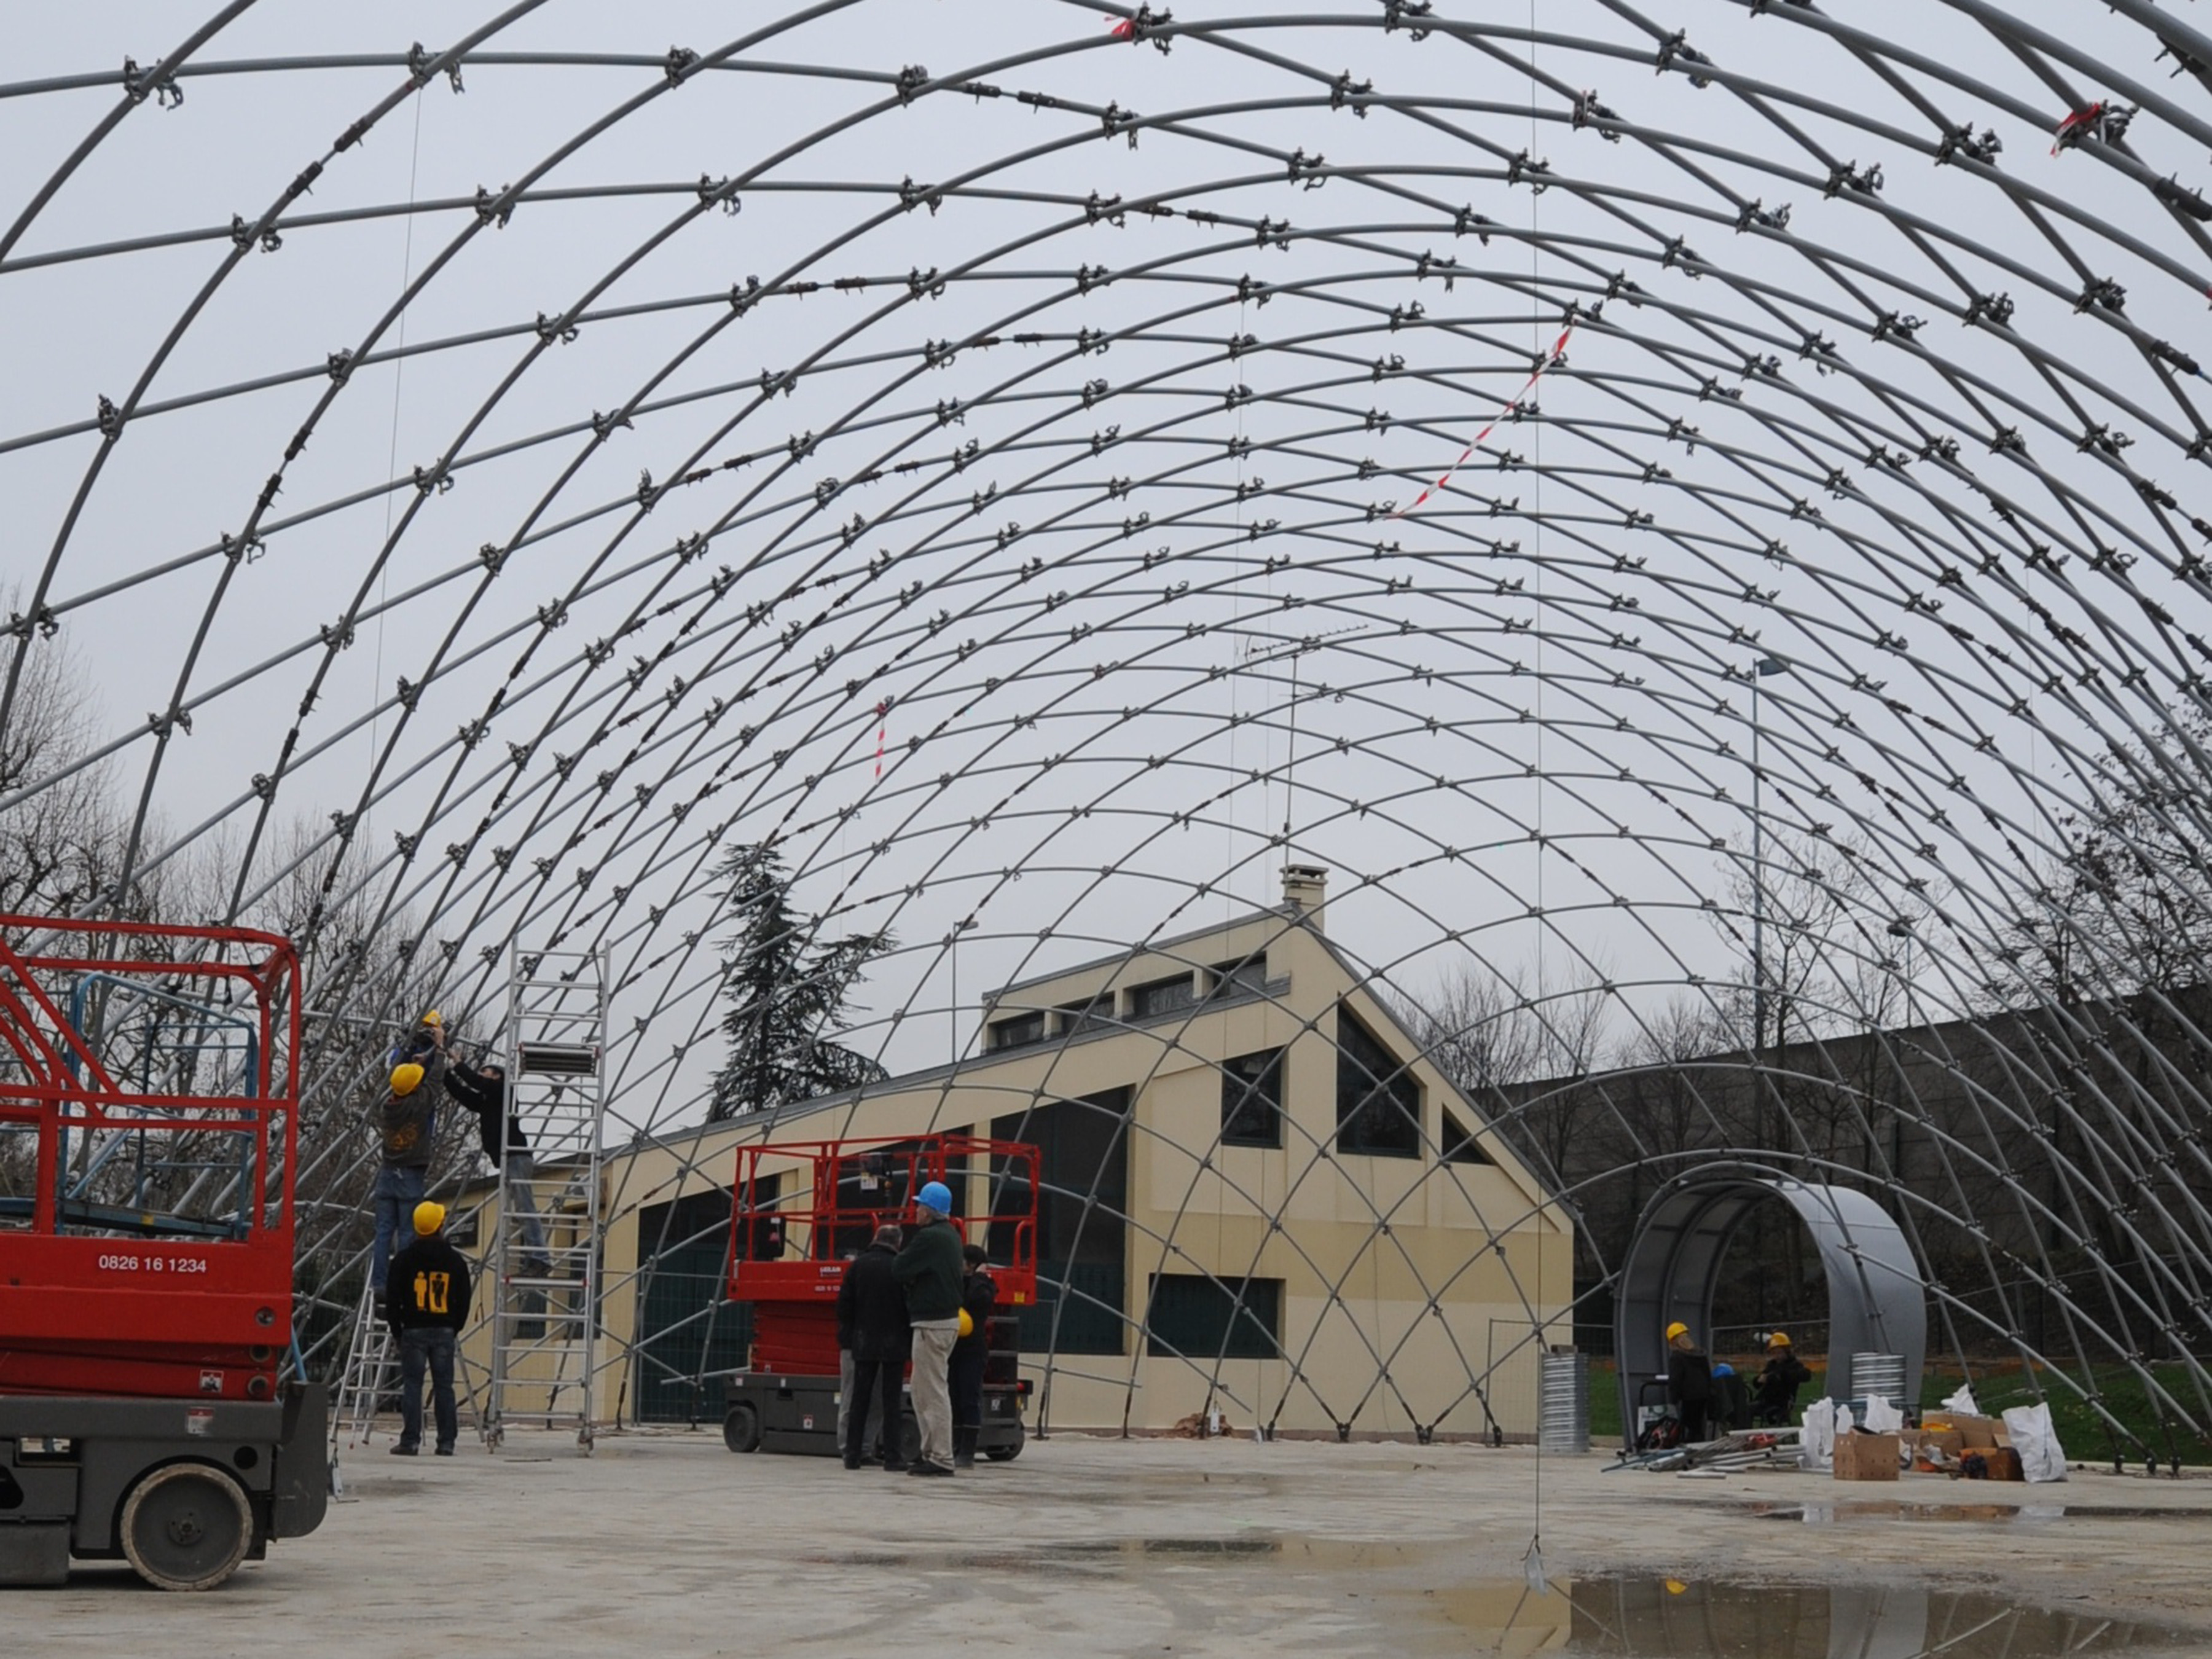
\includegraphics[width=0.48\textwidth]{cp_4.jpg}\label{fig:cp_4}} \\
% 		%
% 		\subfloat[][Grid is braced]{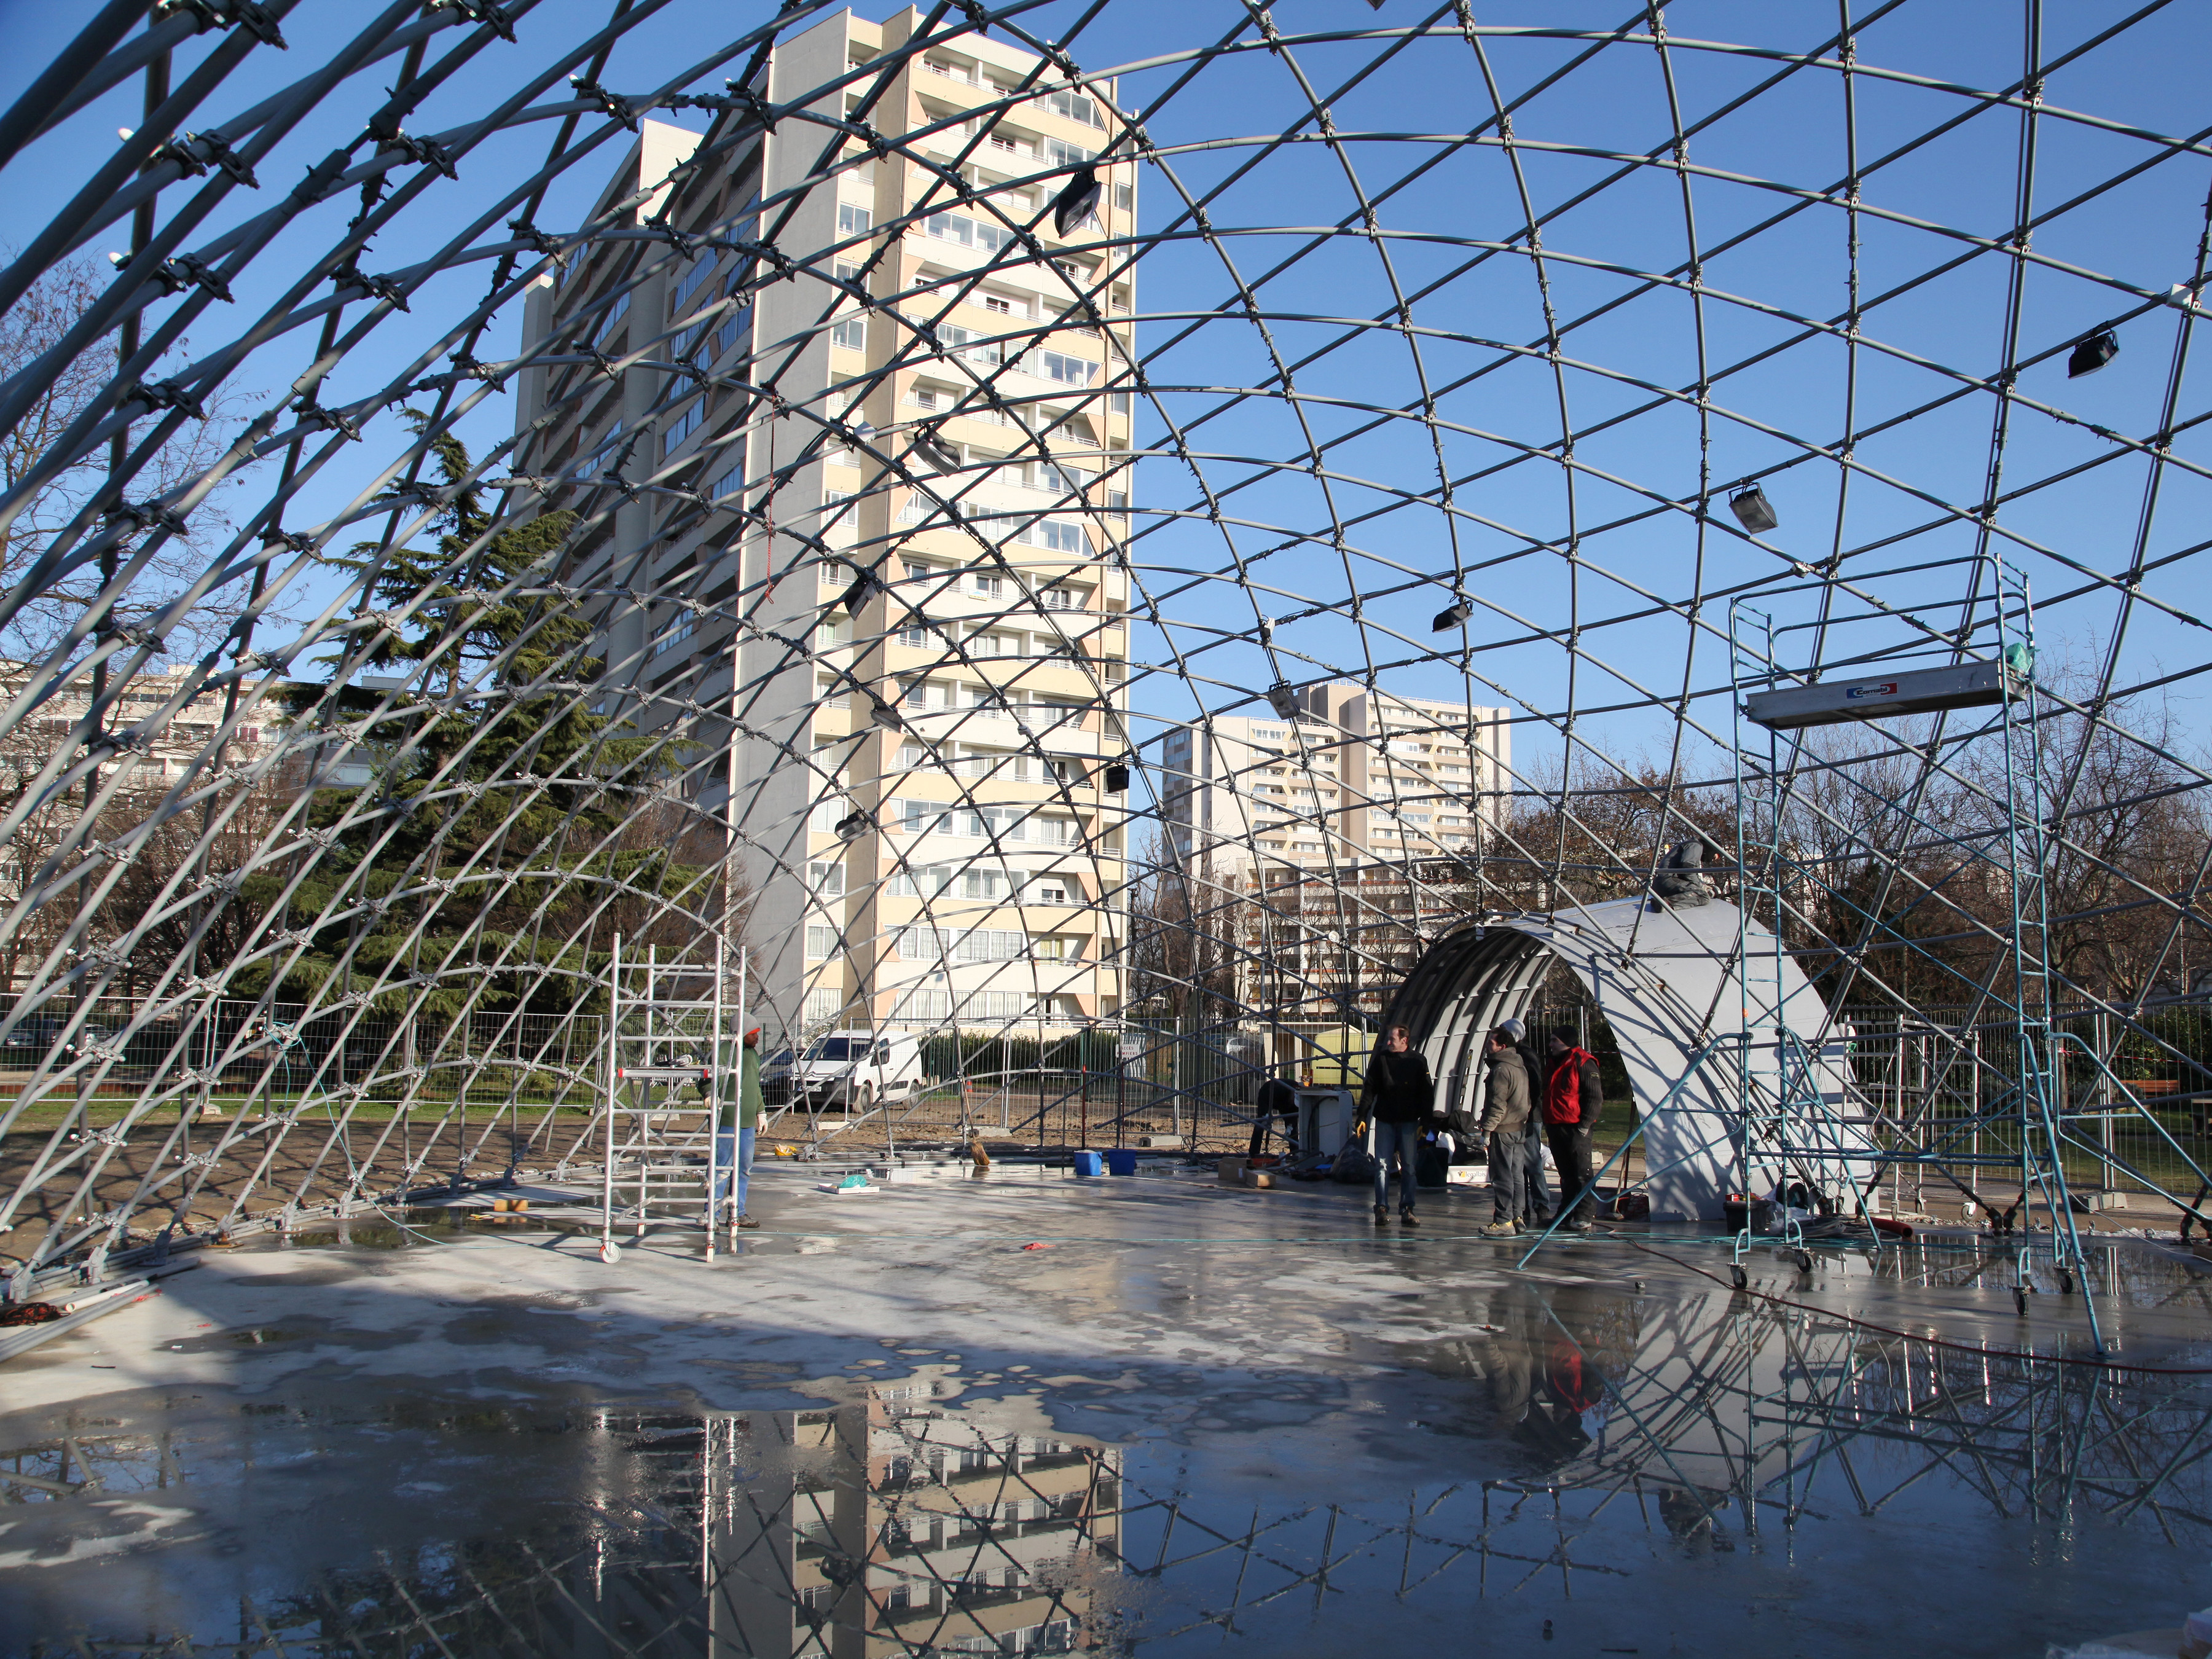
\includegraphics[width=0.48\textwidth]{cp_5.jpg}\label{fig:cp_5}}
% 		\hspace*{\fill}
% 		\subfloat[][Membrane]{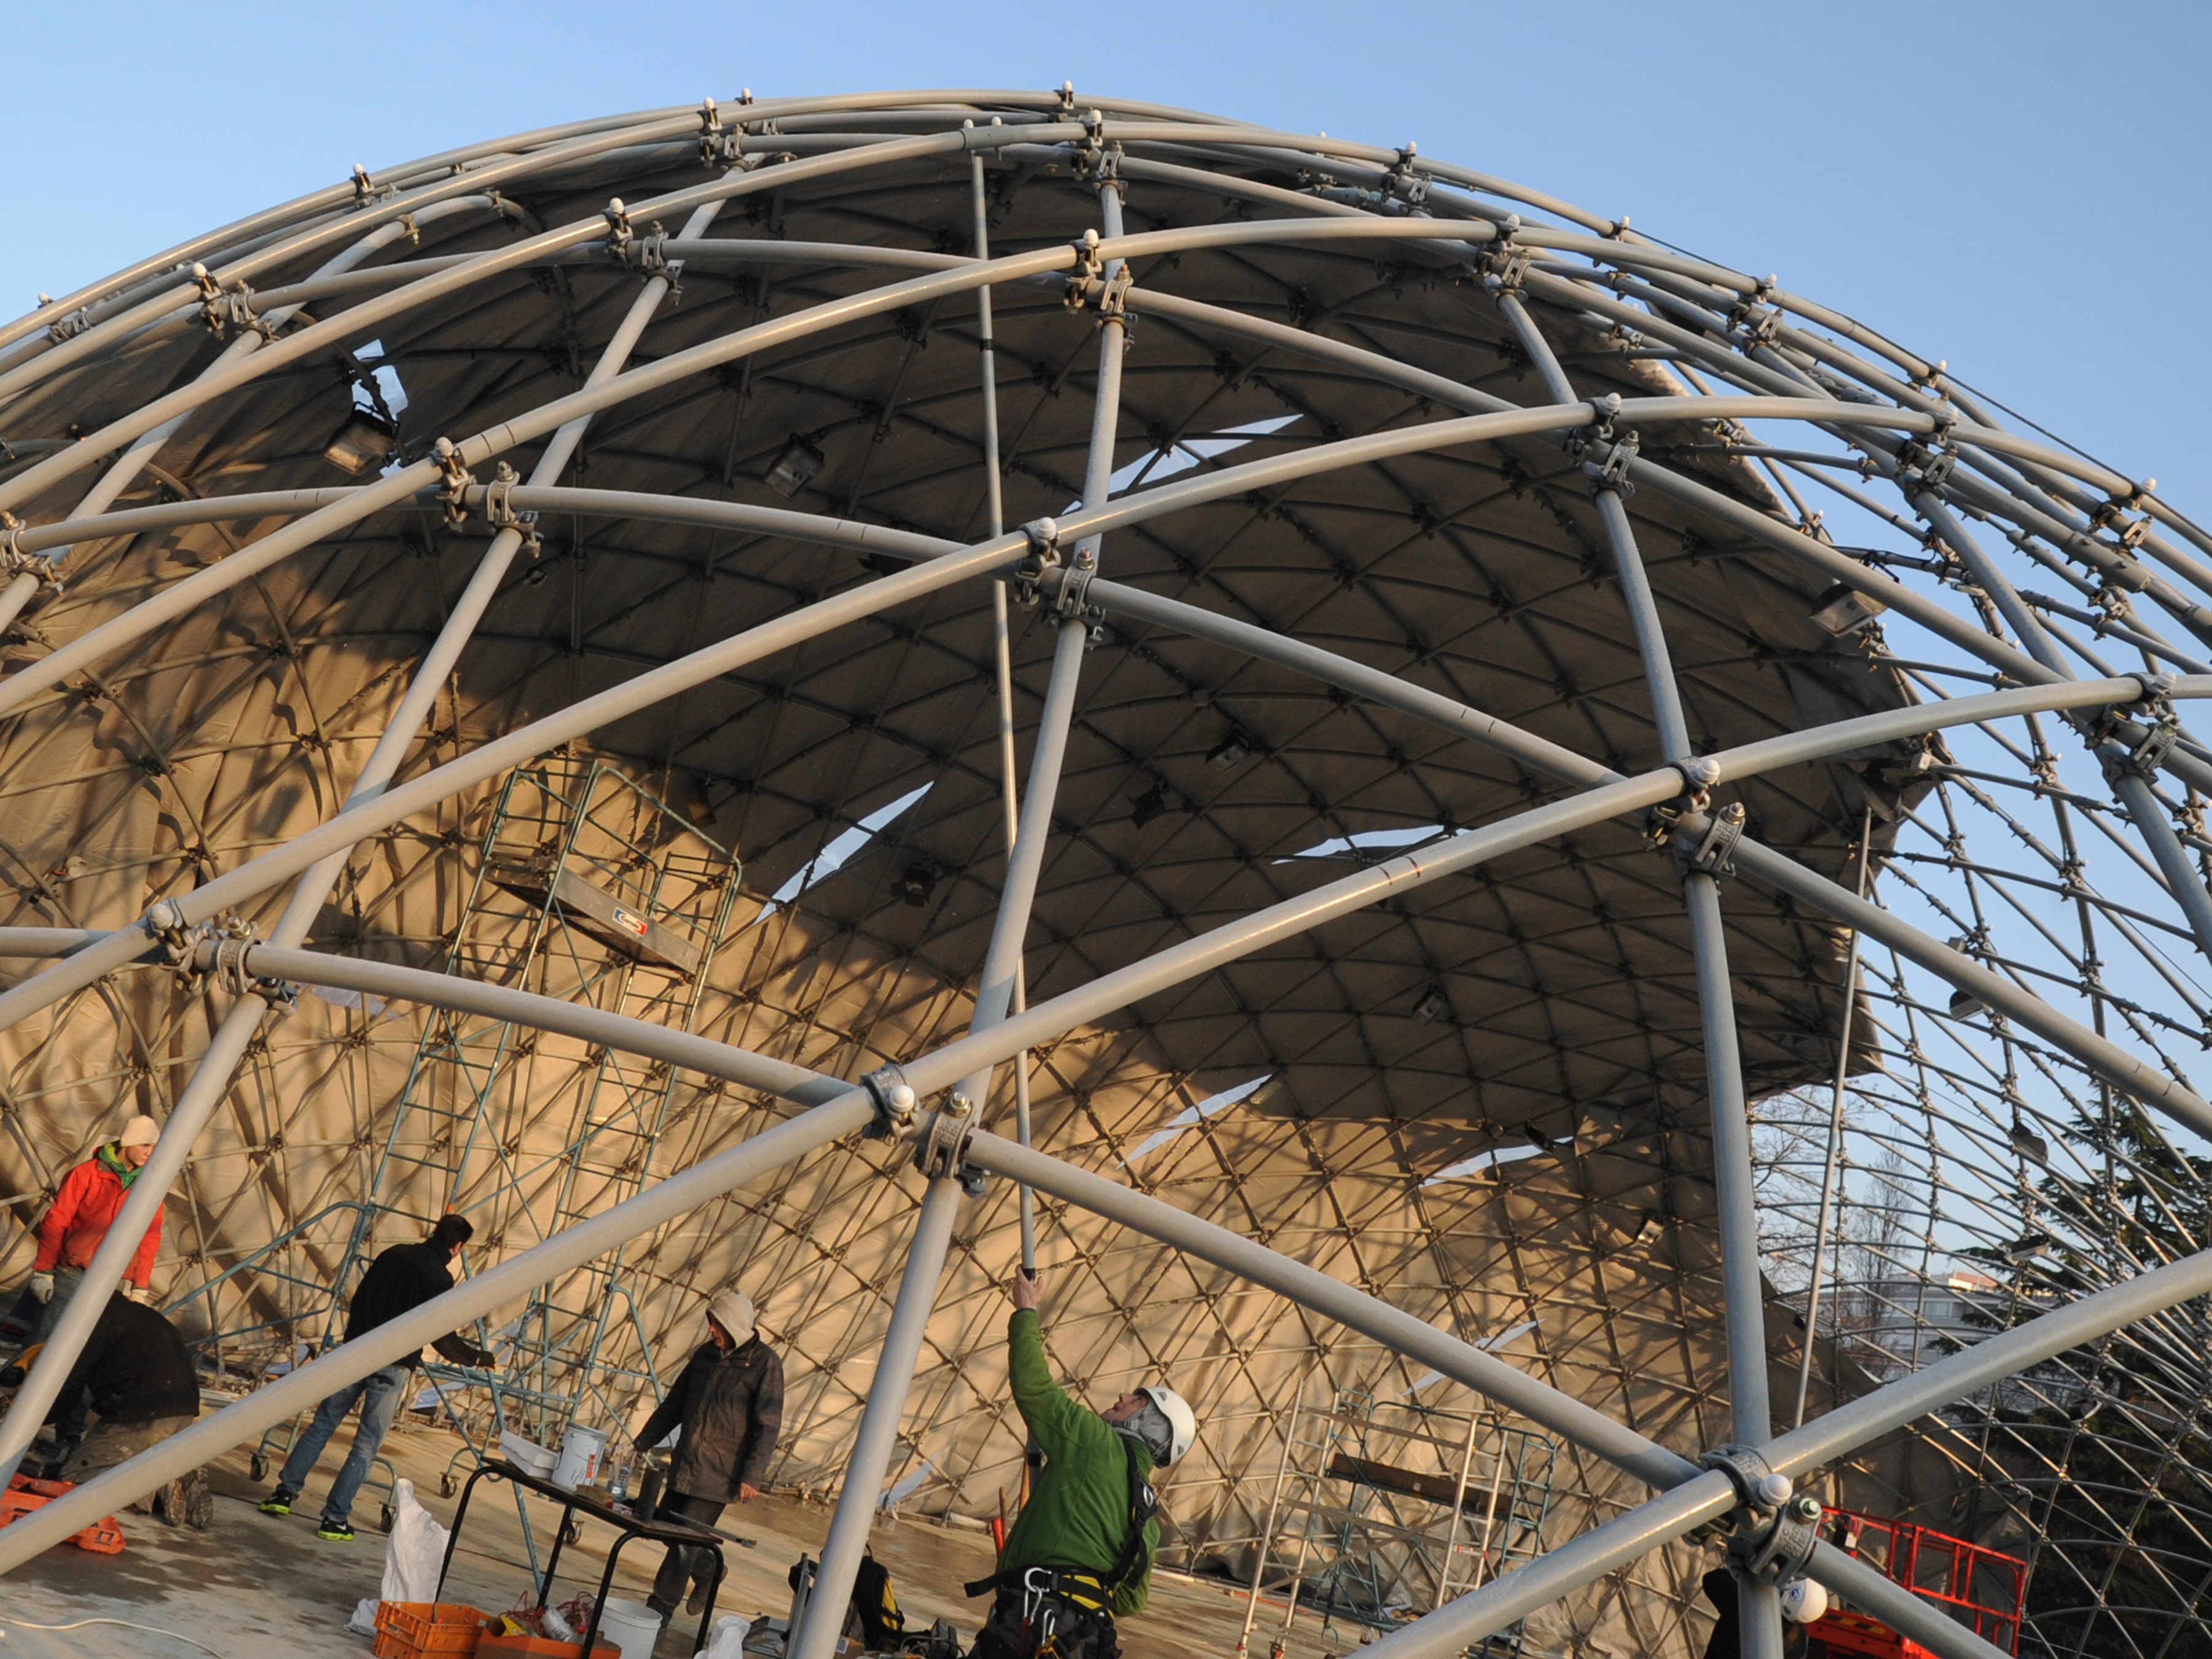
\includegraphics[width=0.48\textwidth]{cp_6.jpg}\label{fig:cp_6}} \\
% 		%
% 		\vspace{10pt}
% 		\caption{Construction process of the gridshell.}
% 		\label{fig:erection}
% 	\end{fullpage}
% \end{figure}

\subsection{Covering of the gridshell}
Finally, the structure is covered with a PVC coated fabric. The membrane comes rolled up. The roll is positioned at one side. Then it is progressively unrolled toward the other side (see \cref{fig:cp_6}). This step requires professional rope workers. Once the membrane is in place, it is hand tensioned with a system of halyard and strap (see \cref{fig:edge}). All included, this stage lasted no more than a single day for a team of six workers.

This step appears as the moment of truth~: if the membrane perfectly fits the gridshell, making no crease, that means the structural analysis was successfully conducted with the required accuracy (see \cref{sec=form-finding}).

%\clearpage
\section{Structural design}\label{sec=proj_design}
%=================

In this section, we exhibit a methodology to design a gridshell with a shape-centered approach. This is one of the key originality of this work and it was first implemented for the Solidays gridshell in 2011. The idea is to identify a grid and a set of supports that once the grid is bended and anchored to its foundations has a geometry as close as possible to the target shape designed by the architect.

Solving this inverse problem is quite a challenge. It requires a lot of back-and-forth between architects and engineers about the definition of the shape. To build a suitable solution the designers need agile tools to get deep insights quickly and adapt their design iteratively until convergence is reached. Unfortunately, existing structural analysis softwares are more validation tools than agile design tools. Although they are necessary to fully validate the feasibility of a given structure, they are quite limited to explore the space of solutions.

The presented methodology tackles this issue by providing appropriate design criteria to the designer. These criteria can be implemented in real-time softwares, thus approaching the agility of the physical models employed in the past \cite{Addis2013}.

\subsection{Overall design process}
%------------------------------------------

The goal of the design process is to identify a gridshell structure that works and respects as faithfully as possible the architectural project with respect to the shape and program. The design of the gridshell represents \textquote{the path from shape to structure}. Its progress is iterative and revolves around three major stages~:
\begin{itemize}
\item shape : modeling a shape from the architectural brief
\item mesh : meshing the shape to obtain the geometry of the grid
\item structure : analyze the structural efficiency of the grid
\end{itemize}
Developing this structural design was a complex process. Indeed, for each step, the method, the tool and the criteria that offer both a sufficient explorative richness in order to find potential candidate solutions, and the means to evaluate and compare the suitability of those solutions, had to be found. In the next part of this section, the studied options and the selected evaluation criteria for each previously mentioned stage are presented.

\subsection{3D modelling of the intended shape}
%------------------------------------------
The first step of the process consists in building a precise geometric model from the sketch of the architect and evaluating its mechanical potential (see \cref{fig:shape_bench}). At this stage, the goal is to estimate quickly the probability that a given shape would lead to the generation of a structurally feasible gridshell.

Stresses in the grid are mainly due to the bending of the tubes. Therefore, they can be derived directly from the measurement of the geometric curvature of the tubes. Because the principal curvatures of the surface give a quantitative measurement of the local curvature of any curve drawn on a surface, they are relevant indicators to evaluate the stress rate of laying a grid on the said surface.\footnote{Indeed, any normal section of the surface will have its curvature bounded by the principal curvatures of the surface. Therefore this seems reasonable to seek grids that fulfill this criterion as the structural elements would probably not resist too large variations of curvatures in the plane of the surface.} Particularly, the following condition has to be satisfied everywhere~:
\begin{equation}
	\mathrm{E} \cdot \frac{r}{R_{min}} < \frac{\sigma_{k,flex}}{\gamma_{lt}}
	\label{eq:crit_1}
\end{equation}
where $r$ is the tube’s outer radius, $R_{min}$ is the minimum principal radius of curvature of the surface, $E$ is the flexural modulus, $\sigma_{k,flex}$ the characteristic flexural strength and $\gamma_{lt}$ the long-term partial coefficient of material resistance (see \cref{sec=safety}).

Ideally, the shape is controlled by few key parameters. Thus, it is easier to adapt and optimize the shape through an iterative process towards the above criterion \cref{eq:crit_1}.

\afterpage{%
	\AddToShipoutPictureBG*{% 
		\Photo[
			node=CAtl,
			anchor=north west,
			xshift=0mm,
			gopt={width=\textwidth},
			]{curvature_analysis.jpg}%
		\savenodes{A}
		\intersectnode{CAtl |- Abr}{Pt}
		\PhotoCaptionRef[
			hrefnode=Atl,
			node=Atr,
			anchor=south east,
			yshift=\PhotoRefSkip,
			phantom=true,
			]{figure}{}{Benchmarking shapes regarding their curvature}{fig:shape_bench}
		\PhotoTextBox[
			node=Pt,
			anchor=north west,
			yshift=-\PhotoSkip,
			width=10cm,
			border=false,
			]{%
				\figurecaption{fig:shape_bench}
			}
	}
	\setlength{\tmpheight}{\PhotoHeight+\PhotoBigSkip}
	% \addtolength{\tmpheight}{\PhotoBigSkip}
	\hbox{\vspace{\tmpheight}}
}

% \begin{figure}[t]
% \centering
% %\begin{fullpage}
% 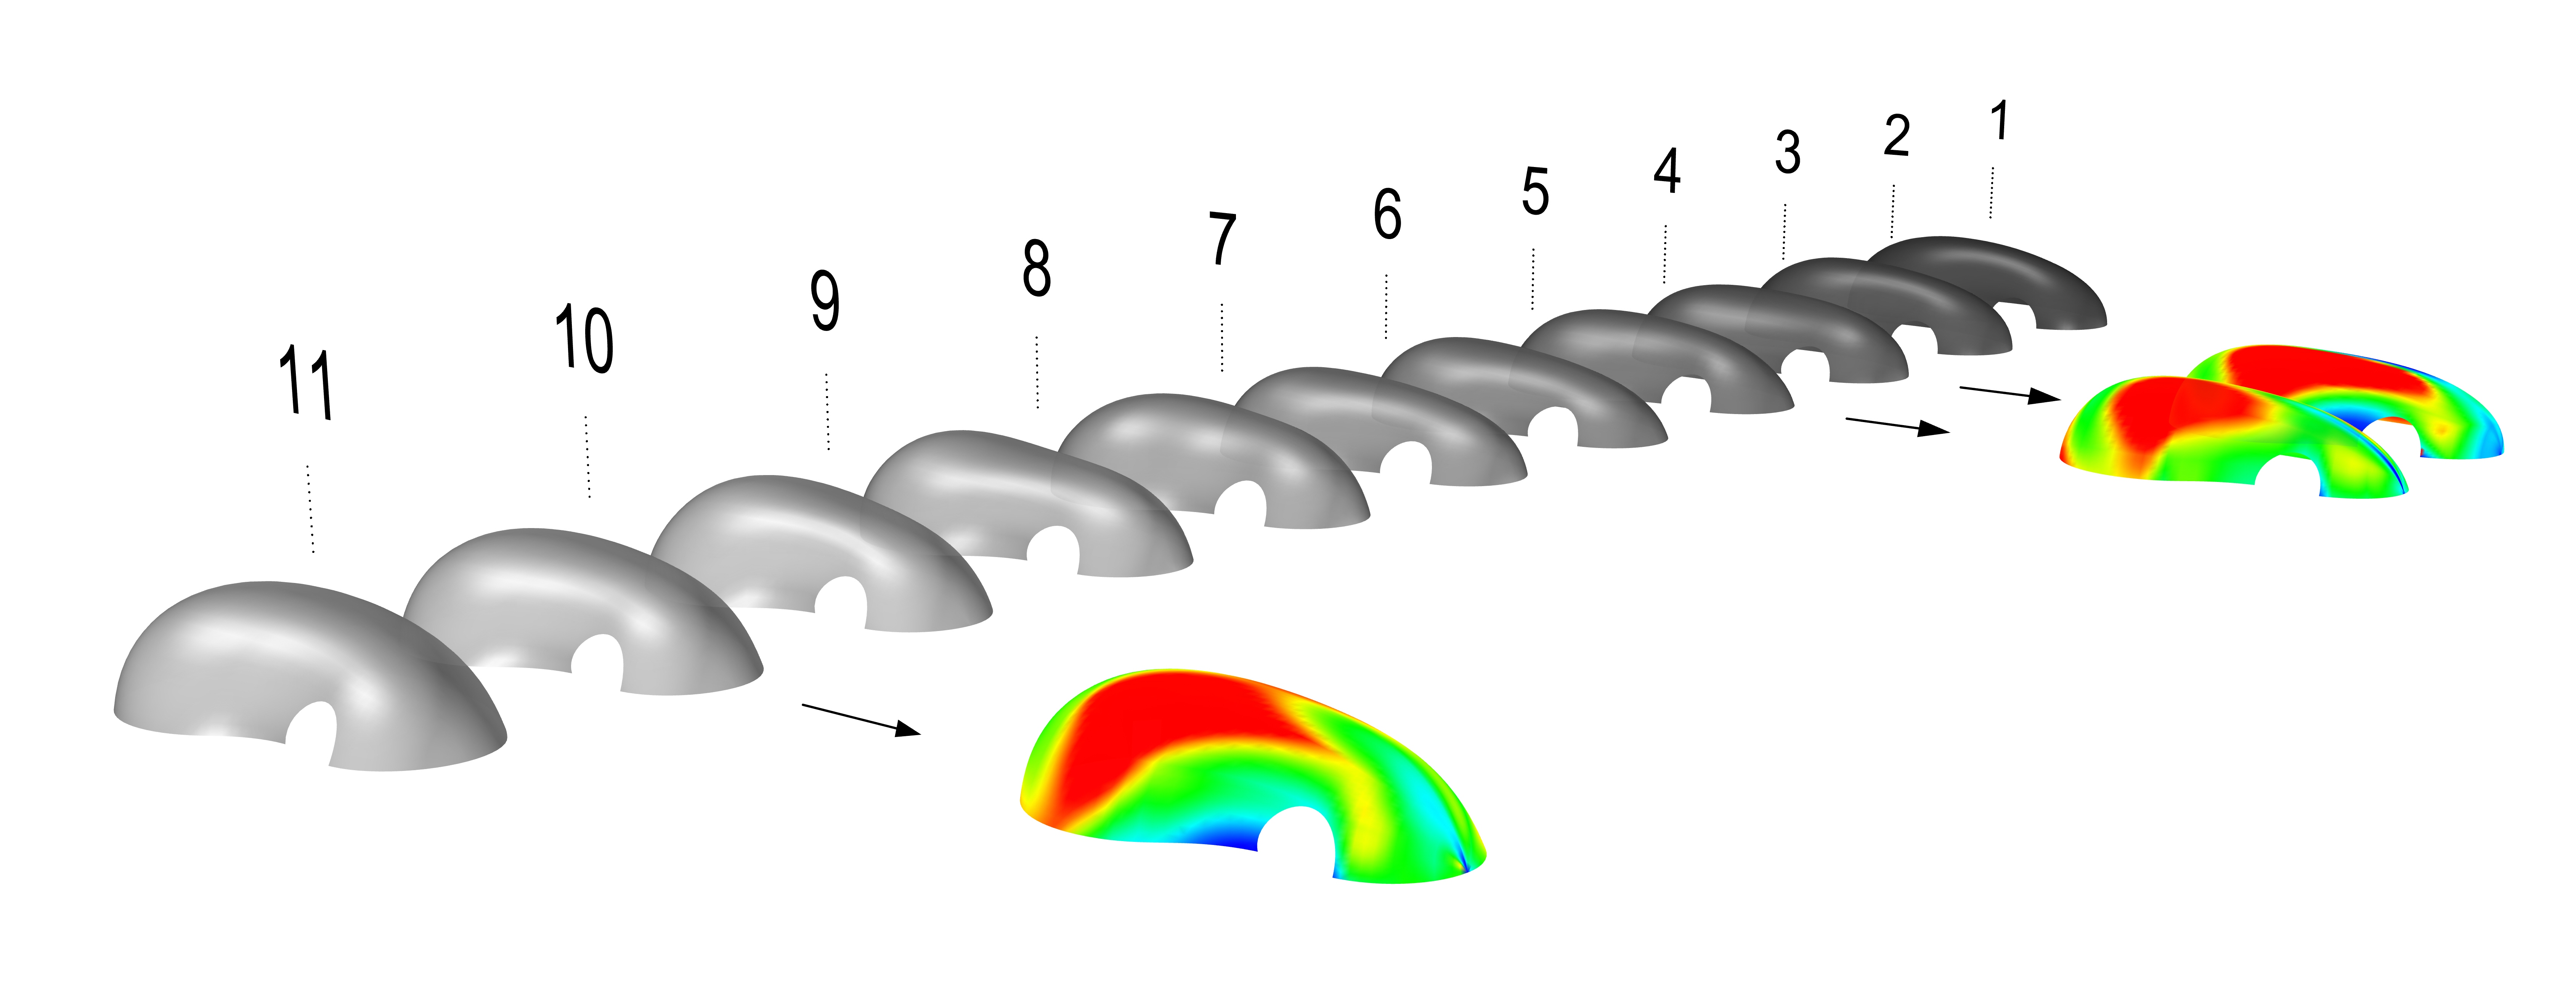
\includegraphics[width=\textwidth]{curvature_analysis}
% \caption[Benchmarking shapes regarding their curvature]{Benchmarking shapes regarding their minimum principal curvature.}
% \label{fig:shape_bench}
% %\end{fullpage}
% \end{figure}

\subsection{Meshing the surface}
%------------------------------------------
During the second step, the candidate surface is meshed and the mechanical potential of the resulting grid is evaluated. At this stage, the probability of a given mesh leading to the generation of a viable gridshell structure is estimated. Simultaneously, meshes are compared according to their architectural relevance.

In this step, the geometric curvature of the polylines drawn on the surface is an appropriate criterion to characterize the mechanical potential of the grid. Unlike the previous step, this criterion takes into account the curvature of the studied mesh and not the minimum principal curvature. In particular, it has to be ensured that the following condition is satisfied everywhere~:
\begin{equation}
	\mathrm{E} \cdot   \frac{r}{R_{spline}}  <   \frac{\sigma_{k,flex}}{\gamma_{lt}}
	\label{eq:crit_2}
\end{equation}
where $R_{spline}$ is the spline’s local curvature radius. The mesh is obtained by the compass method (see below), which develops a regularly spaced grid on a surface from two secant curves lying on the surface and called \emph{directrix}. I implemented this method, proposed by \citet{IL10}, for the Solidays gridshell in 2011 \cite{DuPeloux2011}.\footnote{This method was also used at the laboratoire Navier by \citef{Bouhaya2014} and more recently by \citef{Masson2017b}.} The method guarantees that the grid is made of parallelograms when developed in a plane. This geometric property is exactly what we are looking for to ensure the necessary degree of freedom of the grid responsible for its deployment (see \cref{sec=swivel}). For a given shape, there are an infinite number of possible meshes. The goal of the method is to identify at least one grid which satisfies both the architectural and the structural requirements.

% \begin{figure}[t]
%      	\centering
% %	\begin{fullpage}
% 		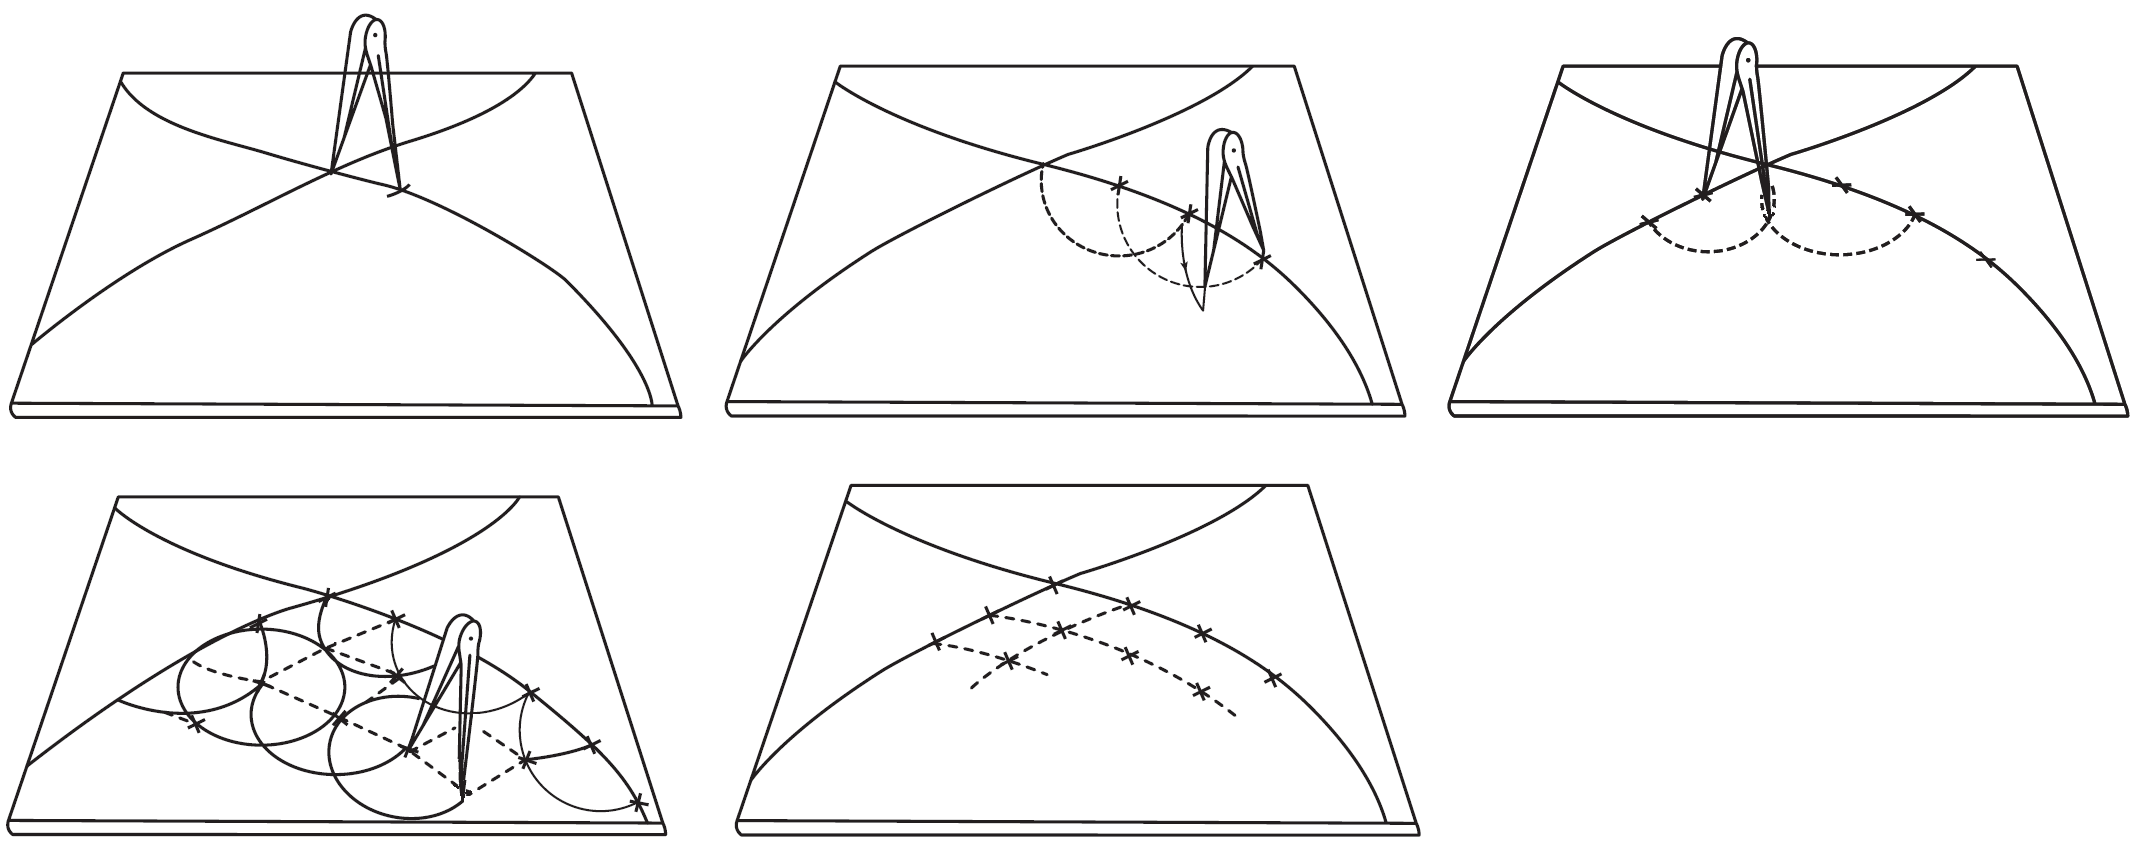
\includegraphics[width=0.8\textwidth]{compass_method.png}
% 		\caption[How the compass method works]{How the compass method works.}
% 		\label{fig:compass_method}
% 		%
% 		\vspace{0.75cm}
% 		%
% 		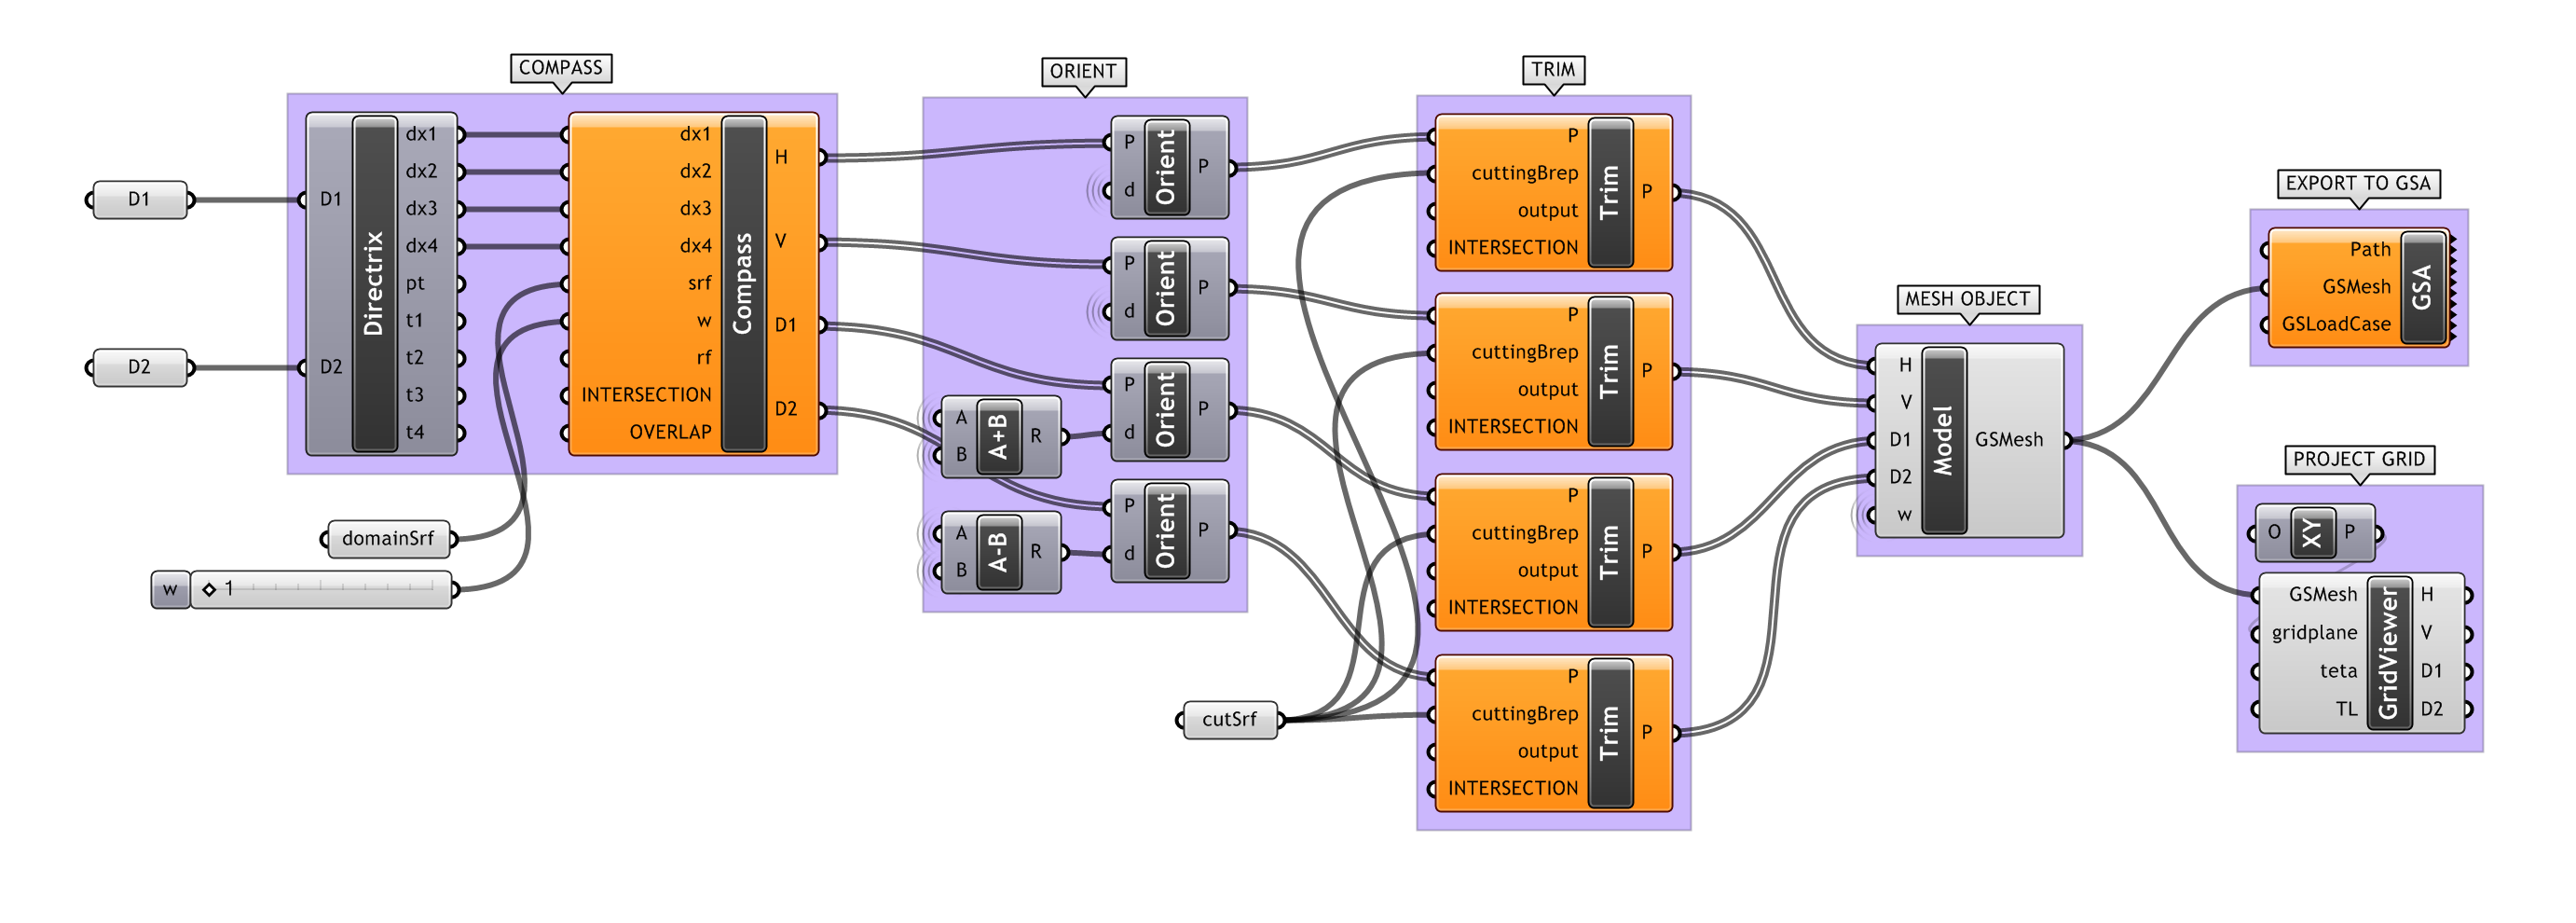
\includegraphics[width=1\textwidth]{canevas.png}
% 		\caption{Meshing software as a plugin for \emph{Grasshopper}.}
% 		\label{fig:canevas}
% %	\end{fullpage}
% \end{figure}

\subsubsection{Compass method}\label{sec=compass}
This process propagates a two way mesh of constant pitch on any NURBS surface (see \cref{fig:compass_method}). Two secant directrices are drawn on the surface to mesh. These curves mark the boundary of four quadrants. Each half directrix is then subdivided with a compass of constant distance (the pitch). Finally, from two consecutive half directrix quadrants are meshed with the same compass distance.

The compass method does not allow to spread the mesh everywhere on a given surface because it stops when a directrix reaches the boundary of the surface. Only a portion of the surface can be meshed and the covered area varies according to the chosen set of directrices. To overcome this difficulty, we consider the gridshell surface (see \cref{fig:compass_a}) as a part of a larger domain surface (see \cref{fig:compass_c}). Trimmed by a plane, this domain surface should give back the intended shape to build (see \cref{fig:compass_b}). Therefore, it is possible to mesh the domain surface (see \cref{fig:compass_d}) and to retrieve a Chebyshev net (that is an equilateral mesh) that cover completely the initial surface (see \cref{fig:compass_f}).

The method is easily extended to meshes with variable pitch. This idea was explored to find optimal grids with genetic algorithm by \citet{Bouhaya2014}. It is worthwhile to mention an attempt to extend this method for multilayer Chebyshev grids by \citet{Lefevre2015}.

\blankpage{
	\hbox{}\thispagestyle{empty}
	\setlength{\tmpwidth}{6cm}
	\AddToShipoutPictureBG*{%
		%%
		\intersectnode{PPtr |- CAtl}{Pt}
		\Photo[
			node=Pt,
			anchor=north east,
			gopt={width=\tmpwidth},
			]{compass_3.png}%
		\savenodes{C}
		\Photo[
			node=Ctl,
			anchor=north east,
			xshift=-\PhotoSkip,
			% yshift=\PhotoBigSkip,
			gopt={width=\tmpwidth},
			]{compass_2.png}%
		\savenodes{B}
		\Photo[
			node=Btl,
			anchor=north east,
			xshift=-\PhotoSkip,
			gopt={width=\tmpwidth},
			]{compass_1.png}%
		\savenodes{A}
		%%
		\intersectnode{PPtl |- Abr}{Pt}
		\Photo[
			node=Pt,
			anchor=north west,
			yshift=-\PhotoBigSkip,
			gopt={width=\tmpwidth},
			]{compass_4.png}%
		\savenodes{D}
		\Photo[
			node=Dtr,
			anchor=north west,
			xshift=\PhotoSkip,
			% yshift=\PhotoBigSkip,
			gopt={width=\tmpwidth},
			]{compass_5.png}%
		\savenodes{E}
		\Photo[
			node=Etr,
			anchor=north west,
			xshift=\PhotoSkip,
			% yshift=\PhotoBigSkip,
			gopt={width=\tmpwidth},
			]{compass_6.png}%
		\savenodes{F}
		\intersectnode{Ftr |- CAbl}{Pt}
		\Photo[
			node=Pt,
			anchor=south east,
			xshift=0mm,
			yshift=\PhotoBigSkip,
			gopt={width=0.6\textwidth},
			]{compass_method.png}%
		\savenodes{G}
		%%%%%%
		\PhotoCaptionRef[
			hrefnode=CAtl,
			node=Atl,
			anchor=south west,
			yshift=\PhotoRefSkip,
			phantom=true,
			]{figure}{}{The compass method step by step}{fig:stepbystep}
		\PhotoCaptionRef[
			hrefnode=Atl,
			node=Atl,
			anchor=south west,
			yshift=\PhotoRefSkip,
			]{subfigure}{}{Target shape}{fig:compass_a}
		\PhotoCaptionRef[
			hrefnode=Btl,
			node=Btl,
			anchor=south west,
			yshift=\PhotoRefSkip,
			]{subfigure}{}{Domain and trimming surfaces}{fig:compass_b}
		\PhotoCaptionRef[
			hrefnode=Ctl,
			node=Ctl,
			anchor=south west,
			yshift=\PhotoRefSkip,
			]{subfigure}{}{Secant directrices}{fig:compass_c}
		\PhotoCaptionRef[
			hrefnode=Dtl,
			node=Dtr,
			anchor=south east,
			yshift=\PhotoRefSkip,
			]{subfigure}{}{Resulting mesh}{fig:compass_d}
		\PhotoCaptionRef[
			hrefnode=Etl,
			node=Etr,
			anchor=south east,
			yshift=\PhotoRefSkip,
			]{subfigure}{}{Trimmed mesh}{fig:compass_e}
		\PhotoCaptionRef[
			hrefnode=Ftl,
			node=Ftr,
			anchor=south east,
			yshift=\PhotoRefSkip,
			]{subfigure}{}{Final grid}{fig:compass_f}
		\intersectnode{Atl |- Fbr}{Pt}
		\PhotoTextBox[
			node=Pt,
			anchor=north west,
			yshift=-\PhotoBigSkip,
			width=10cm,
			border=false,
			]{%
				\figurecaption{fig:stepbystep}\par
				\figurecaption{fig:compass_a}\par
				\figurecaption{fig:compass_b}\par
				\figurecaption{fig:compass_c}\par
				\figurecaption{fig:compass_d}\par
				\figurecaption{fig:compass_e}\par
				\figurecaption{fig:compass_f}
			}
		%%%
		\intersectnode{Gtl |- CAbr}{Pt}
		\PhotoCaptionRef[
			hrefnode=Pt,
			node=Pt,
			anchor=south west,
			% yshift=\PhotoRefSkip,
			phantom=true,
			]{figure}{}{Principle of the compass method}{fig:compass_method}
		\PhotoTextBox[
			node=Pt,
			anchor=south west,
			% yshift=-\PhotoSkip,
			width=10cm,
			border=false,
			]{%
				\figurecaption{fig:compass_method}
			}
	}
}

\subsubsection{Numerical tool}
Here, a specific program developed by \citet{DuPeloux2011} for \rhino{} and \grasshopper{} allows the generation of this kind of mesh on any non-uniform rational B-spline surface (NURBS). It performs the following elementary operations~: surface meshing with the compass method, trimming, control of the geometry’s integrity and flattening of the grid (see \cref{fig:stepbystep,fig:grid_diff}). The tool also generates automatically a text file, which can be imported into a structural analysis software, containing all the required information to build programmatically the analysis model and then perform the form-finding of the structure (see \cref{fig:canevas}). In particular, an add-on feature facilitates loads application of various complexities (snow, wind, etc.), which is otherwise difficult in conventional analysis softwares for freeform structures. However, the tool does not provide any computation facilities itself and this is exactly the goal of the second part of this thesis.

\subsection{Form-finding and bending prestress}\label{sec=form-finding}
%------------------------------------------
In the previous steps, the initial form was optimized and promising meshes for the materialization of the future gridshell were identified. However, the produced meshes do not take into account any of the mechanical reality, because only geometrical rules were used in their generation. The form-finding step consists precisely in finding the geometry of the grid at mechanical equilibrium, and the corresponding permanent bending stresses. The calculation is performed numerically thanks to a dynamic relaxation algorithm with kinetic damping and comprise the following steps~:
\begin{itemize}
\item The grid is bent by a set of applied displacements from its resting position to the compass position.
\item The grid is then relaxed until it falls in its mechanical equilibrium.
\item Bending stresses of the triangulation are calculated relative to the geometry of the equilibrium.
\item Geometry and bending stresses of the triangulation are re-injected into the model in step~2.
\end{itemize}

\blankpage{
	\hbox{}\thispagestyle{empty}
	\setlength{\tmpwidth}{6cm}
	\AddToShipoutPictureBG*{%
		%%
		\intersectnode{PPtr |- CAtl}{Pt}
		\Photo[
			node=CAc,
			anchor=center,
			gopt={width=0.9\textheight, angle=90},
			]{gsa.png}%
		\savenodes{A}
		\Photo[
			node=CAtr,
			anchor=north east,
			xshift=2\PhotoBigSkip,
			gopt={width=3cm, angle=0},
			]{gsa_scale.png}%
		\savenodes{B}
		\PhotoCaptionRef[
			hrefnode=Atl,
			node=Atl,
			anchor=north east,
			phantom=true,
			% yshift=\PhotoRefSkip,
			]{figure}{}{Permanent bending stresses in the structure under self-weight}{fig:gsa}
		\PhotoTextBox[
			node=CAbl,
			anchor=south west,
			border=false,
			]{%
				\figurecaption{fig:gsa}
			}
	}
	\afterpage{%
		
		\AddToShipoutPictureBG*{% 
			\setlength{\tmpwidth}{(\textwidth-3\PhotoBigSkip)/2}
			\Photo[
				node=CAt,
				anchor=north east,
				xshift=-\PhotoBigSkip/2,
				gopt={width=\tmpwidth},
				]{eccentricity_1.png}%
			\savenodes{A}
			\Photo[
				node=CAt,
				anchor=north west,
				xshift=\PhotoBigSkip/2,
				gopt={width=\tmpwidth},
				]{eccentricity_2.png}%
			\savenodes{B}
			%%
			\PhotoCaptionRef[
				hrefnode=Atl,
				node=Atl,
				anchor=south east,
				yshift=\PhotoRefSkip,
				phantom=true,
				]{figure}{}{Reconstruction of the full 3D geometry}{fig:eccentricity}
			\PhotoCaptionRef[
				hrefnode=Atl,
				node=Atr,
				anchor=north east,
				% yshift=\PhotoRefSkip,
				]{subfigure}{}{Wire frame}{fig:eccentricity_a}
			\PhotoCaptionRef[
				hrefnode=Btl,
				node=Btr,
				anchor=north east,
				% yshift=\PhotoRefSkip,
				]{subfigure}{}{Full 3D}{fig:eccentricity_b}
			\intersectnode{CAtl |- Abr}{Pt}
			\PhotoTextBox[
				node=Pt,
				anchor=north west,
				yshift=-\PhotoSkip,
				width=10cm,
				border=false,
				]{%
					\figurecaption{fig:eccentricity}\par
					\figurecaption{fig:eccentricity_a}\par
					\figurecaption{fig:eccentricity_b}\par
				}
		}
		\setlength{\tmpheight}{\PhotoHeight}
		\addtolength{\tmpheight}{4\PhotoBigSkip}
		\hbox{\vspace{\tmpheight}}
	}
}

Two analysis models were built during this process to study the structure with and without bracing tubes.

The computations were realized with the form-finding module of the software Oasys GSA.\footnote{\url{http://www.oasys-software.com/products/engineering/gsa-suite.html}} It relies on a 6-DOF dynamic relaxation algorithm with either viscous or kinetic damping such as the one introduced in \citeyear{Adriaenssens2000} by \citet{Adriaenssens2000}. In practice, making the computations to converge was a really difficult and time-consuming task, highlighting the necessity of a dedicated form-finding tool with a higher level of interactivity. Moreover, coupling between rotational and translational degrees of freedom can cause ill-conditioning problems, which was already noticed by \citet{Adriaenssens2001}. In the same paper, they proposed a 3-DOF element valid for torsion-free cases. Simpler and faster, it is also a lot more stable. This element was reused and extended later for the form-finding of elastic gridshells in composite materials with complex connections by \citet{Douthe2007}. To tackle numeric instabilities the model had to be simplified~:
\begin{itemize}
\item Connections between elements were modeled as rotation-free joints, enforcing only position constrains with out taking into account the eccentricity between the tubes. This becomes a problem when it comes to evaluating the stability of the gridshell as eccentricity can plays a major role \cite{Lefevre2015}. This is also problematic when determining the production length of the tubes and the position of the anchorages (see \cref{sec=asbuilt}).
\item The triangulation could not be embedded from the start in the model and had to be treated separately and re-injected later on.
\end{itemize}

The form-finding process should not be regarded as a pure computational stage were only the equilibrium shape has to be found while all other design parameters are fixed. Indeed, as the goal is to find a suitable geometry with the most relaxed permanent bending stresses in the structure, this process could itself be employed to explore optimal geometries that will lead to more relaxed static equilibriums. In the present project the supports were allowed to move slightly around their target position by the mean of spring supports with orthotropic stiffness. This allowed to decrease the overall level of permanent bending stress in the tubes while granting very minor changes in the geometry.

Finally the process converges when the shape and the pattern drawn by the mesh are suitable for the architect while the permanent bending stresses are acceptable for the tubes (see \cref{sec=safety}). The end results for this stage are presented in \cref{fig:gsa}. Note the smoothness of the mesh and the convergence of the tubes near the altar. Bending stresses are well distributed and inferior to the maximum design stress allowed (\SI{133}{MPa} in that case). Only few tubes are heavy loaded, in the areas where the curvature is the highest.

\subsection{As-built geometry}\label{sec=asbuilt}
 %-------------------------------------
Although, the eccentricity ($e = \SI{136}{\mm}$) remains small compared with the span of the shell ($l =\SI{17}{m}$), it is not negligible compared with the mesh size ($w = \SI{1.0}{m}$). Thus, the tube lengths and anchorage positions could not be determined with sufficient accuracy without taking into account the thickness of the structural grid due to this eccentricity. The employed method, purely geometrical, assesses that the neutral fibre of the shell is equidistant from the first two layers of pipes. The form-finding is performed only with those two layers. Connection axes has to be parallel to the local normal of the shell surface. This assumption was not exact, but, in this case, gave sufficient accuracy. The red pipe was offset by $-e/2$, the green by $+e/2$ and the blue by $+3e/2$ along the surface normal (see \cref{fig:eccentricity}).
% \begin{figure}[p]
%      	\centering
% 	\begin{fullpage}
% 		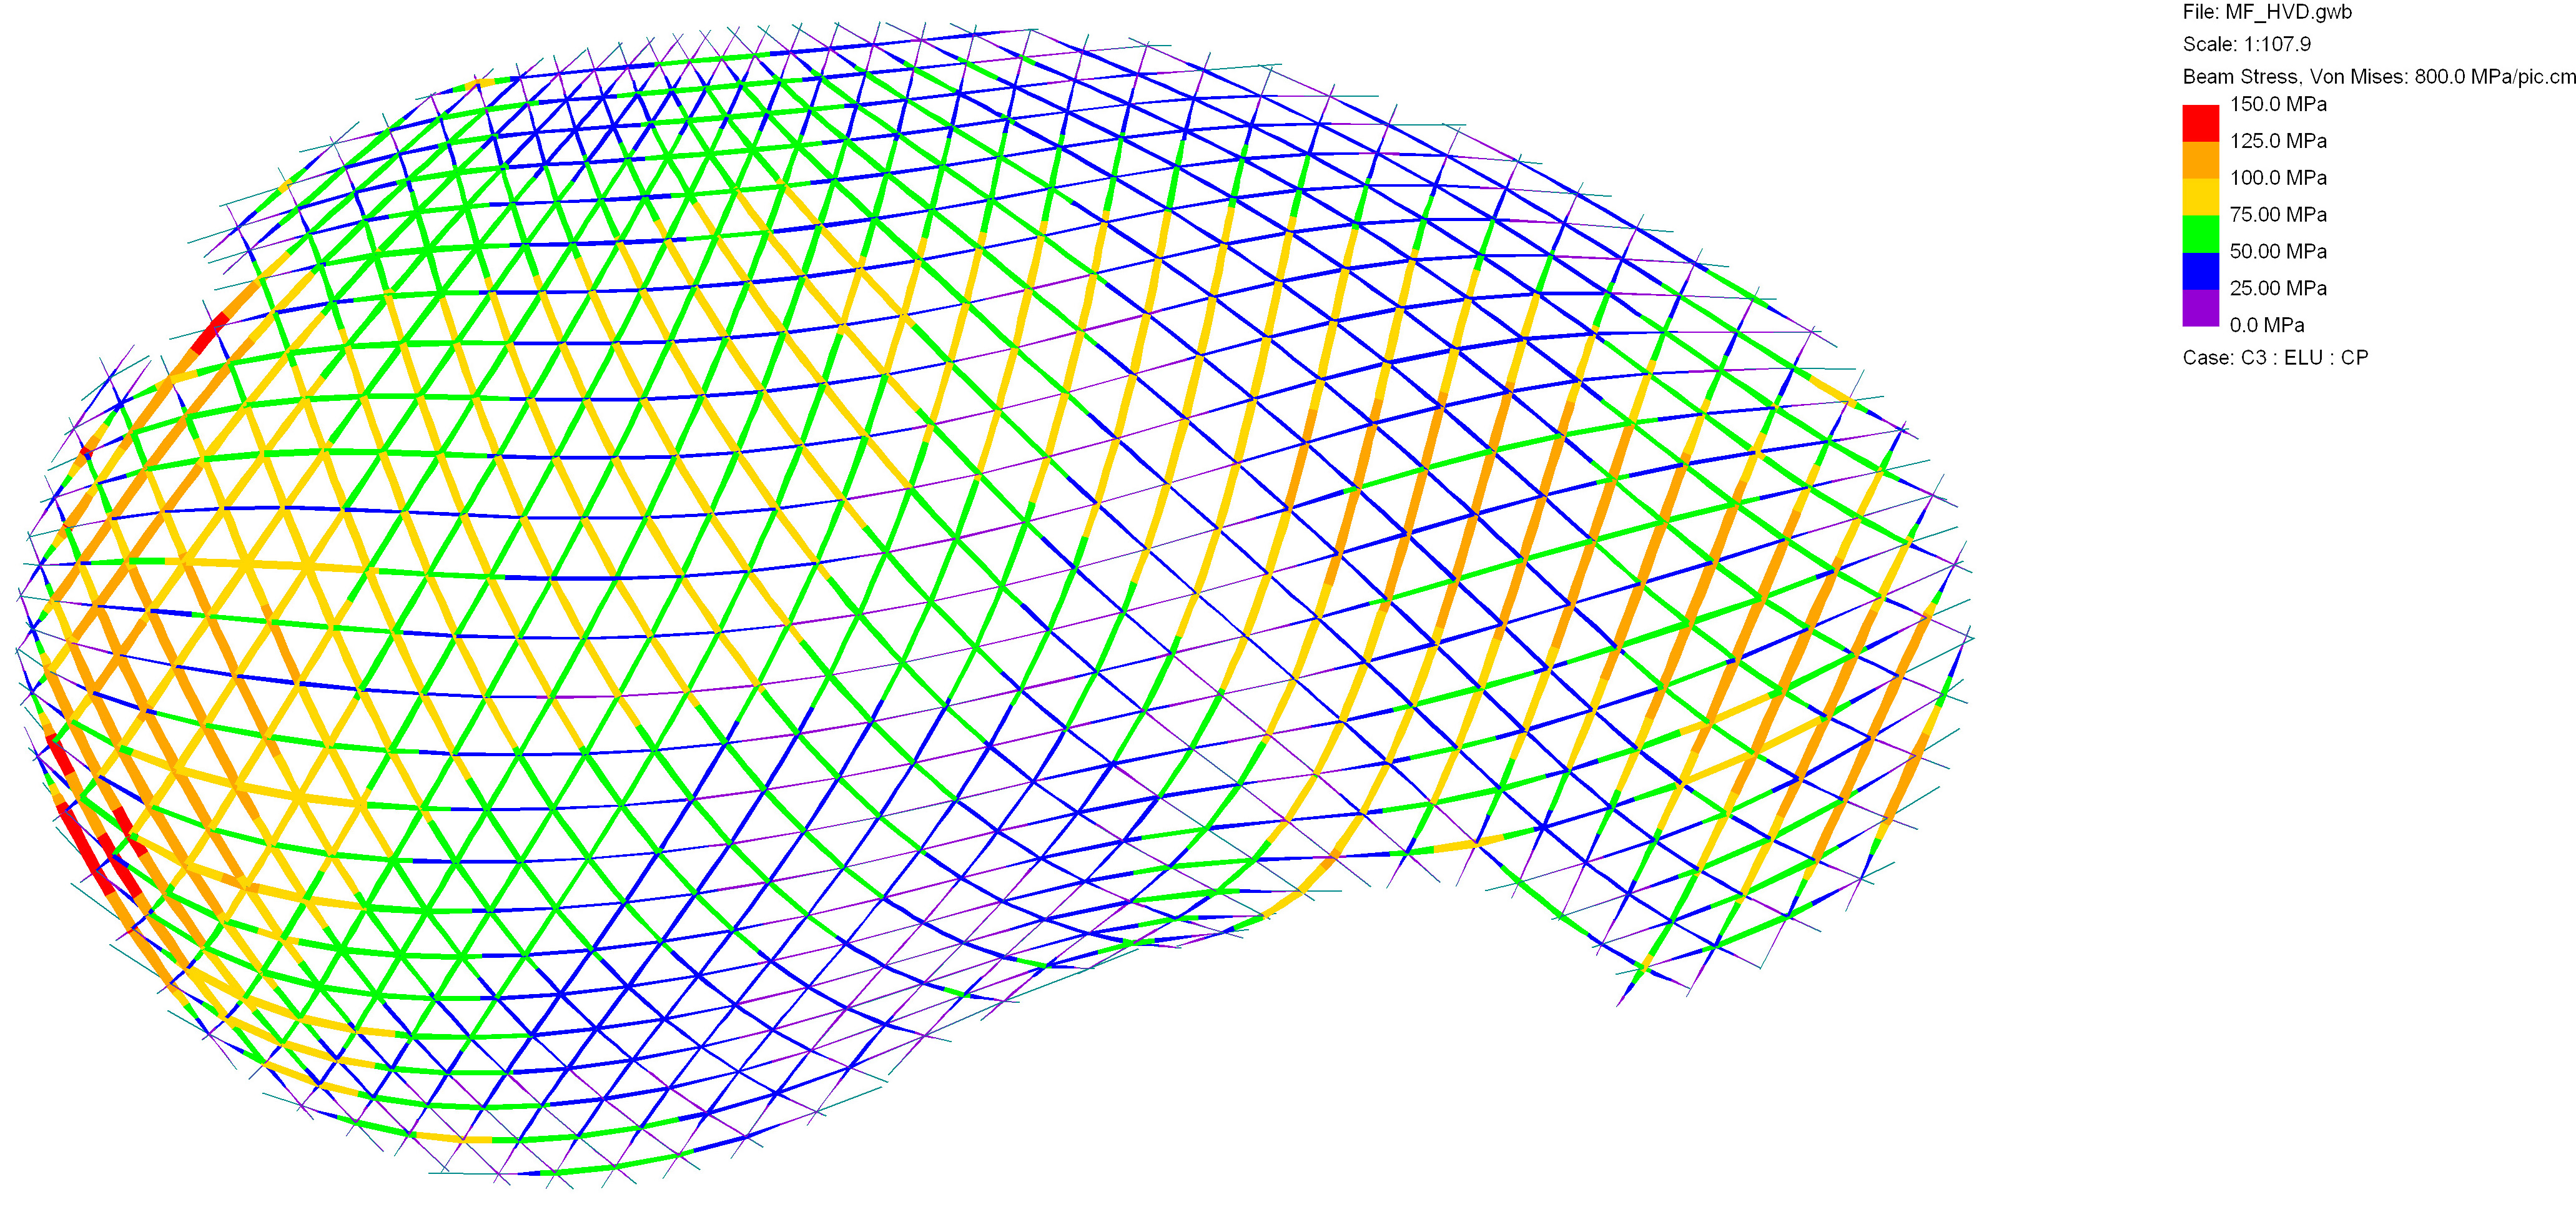
\includegraphics[width=1\textwidth]{gsa2.jpg}
% 		\caption[Permanent bending stresses in the structure under self-weight]{Permanent bending stresses in the structure under self-weight (max = \SI{130}{MPa}).}
% 		\label{fig:gsa}
% 		%
% 		\vspace{1.5cm}
% 		%
% 		\subfloat[][Wire frame]{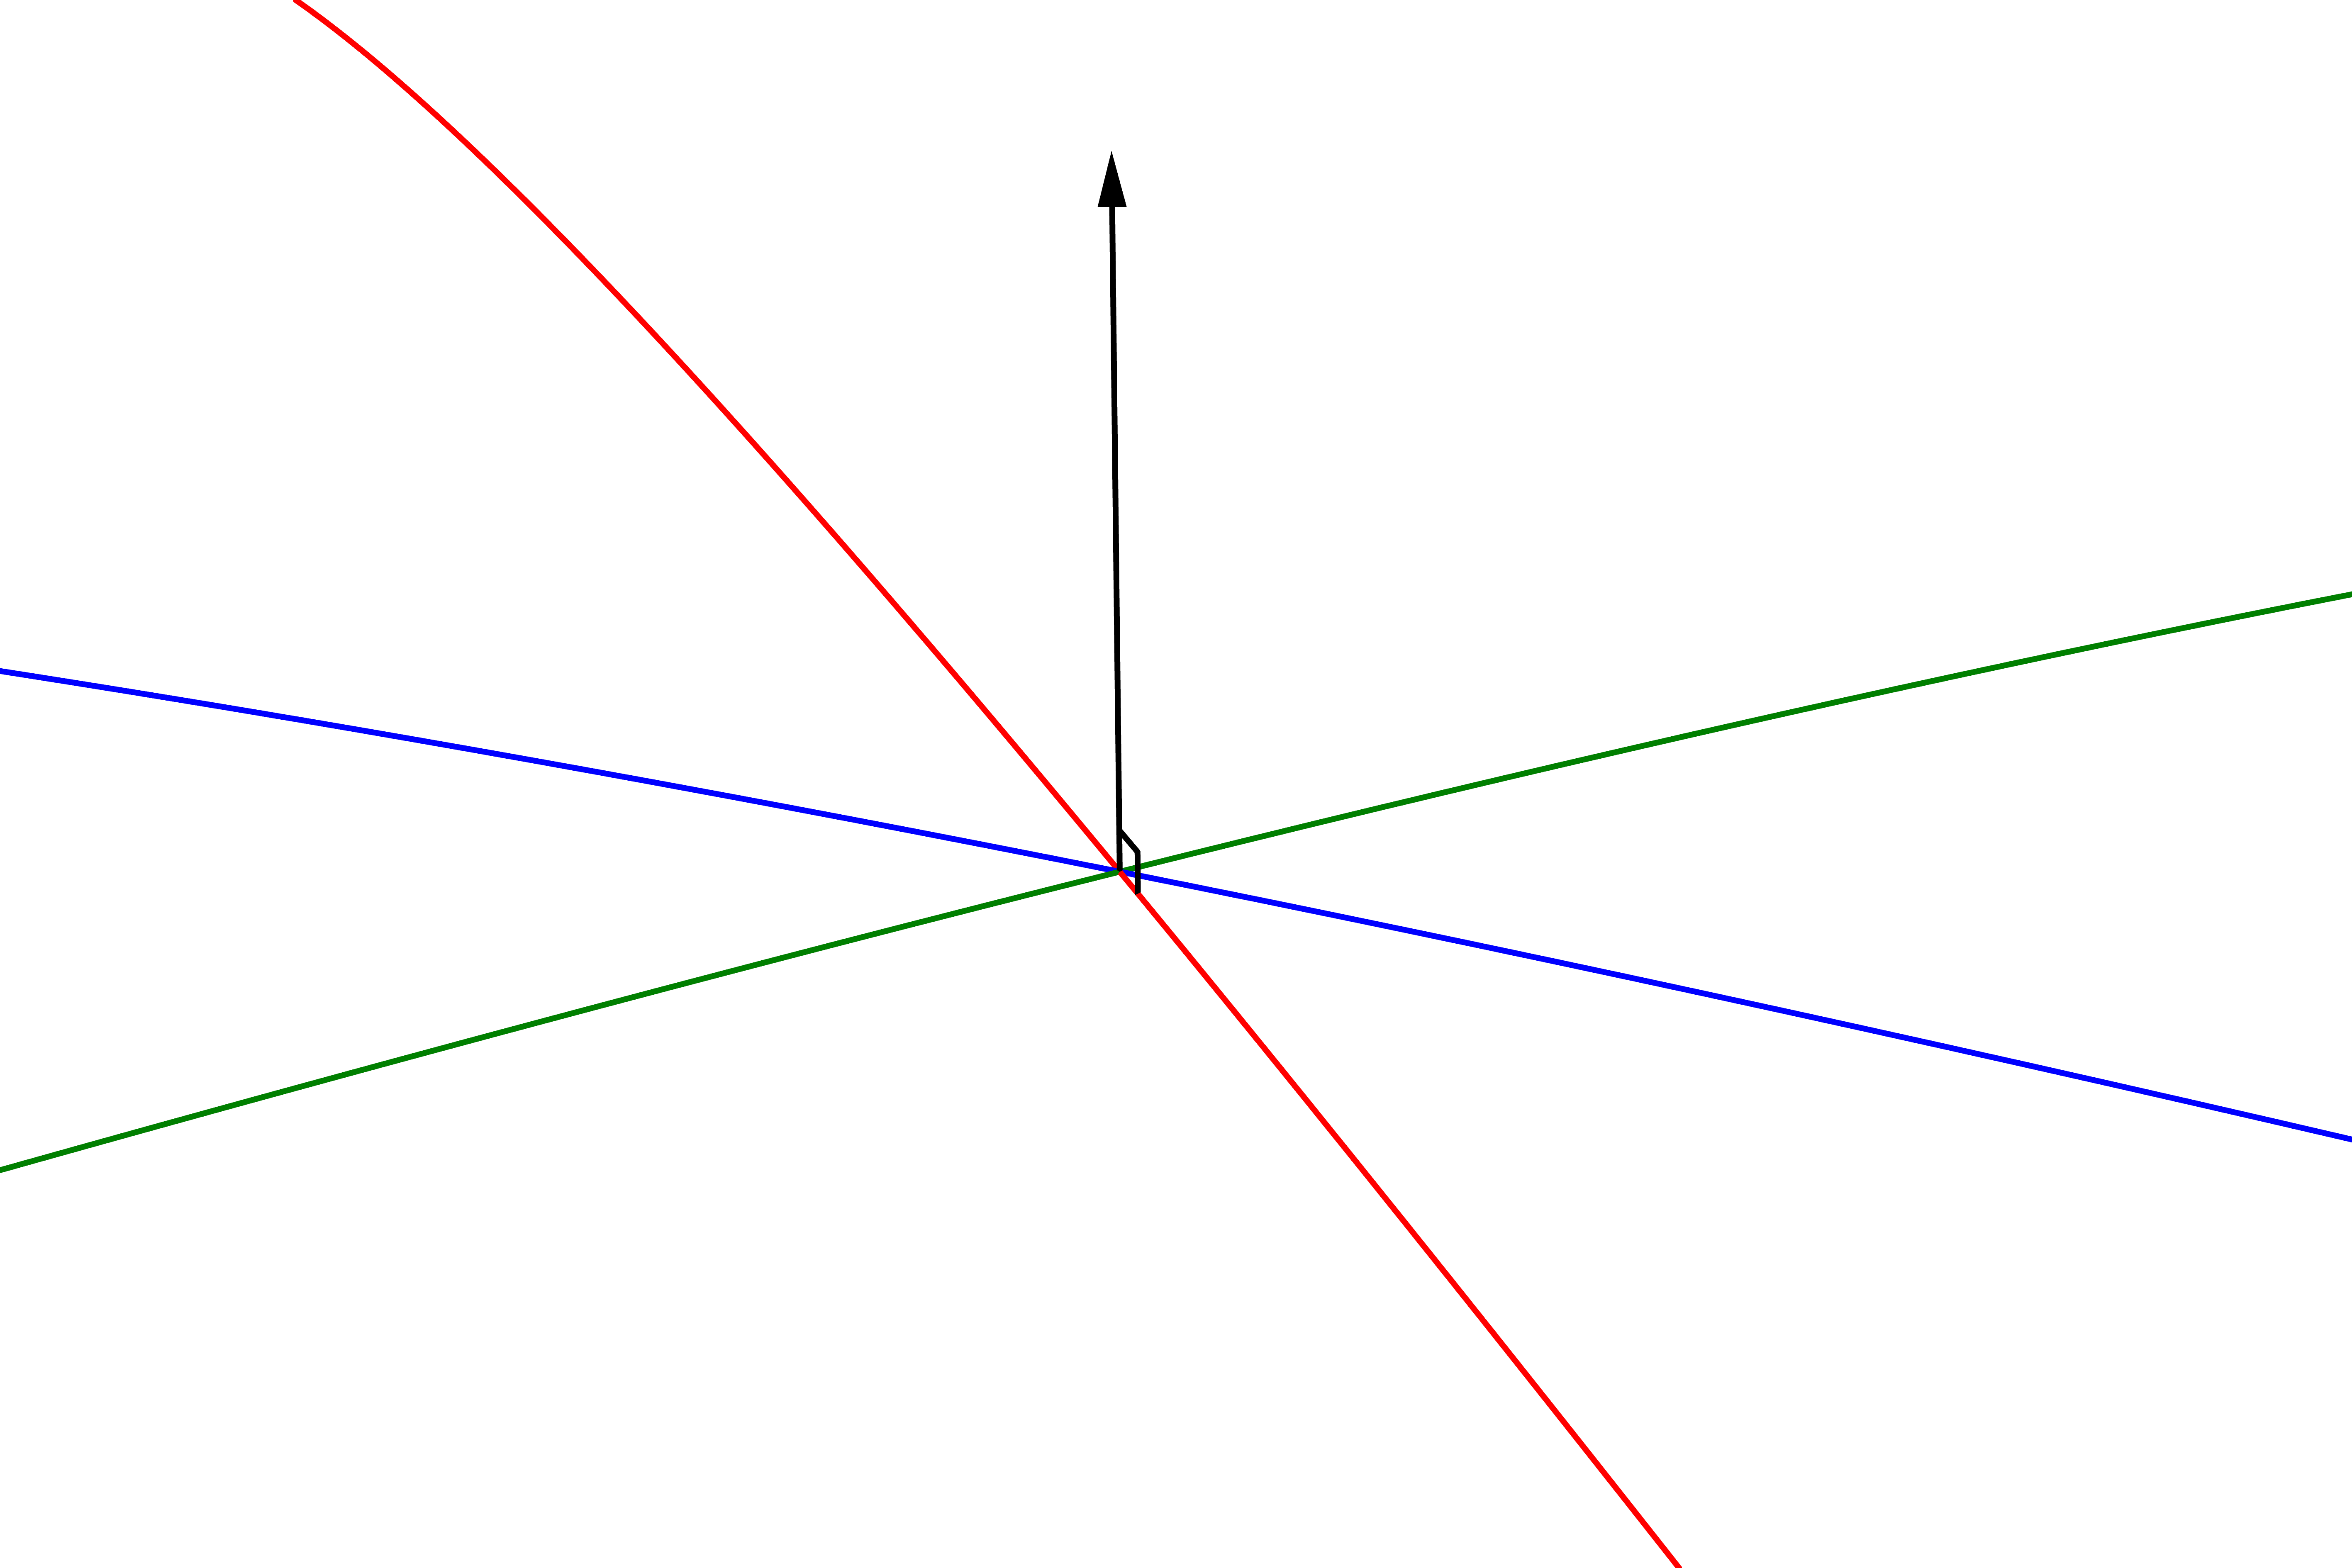
\includegraphics[width=0.48\textwidth]{eccentricity_1.png}\label{fig:eccentricity_a}}
% 		\hspace*{\fill}
% 		\subfloat[][Full 3D]{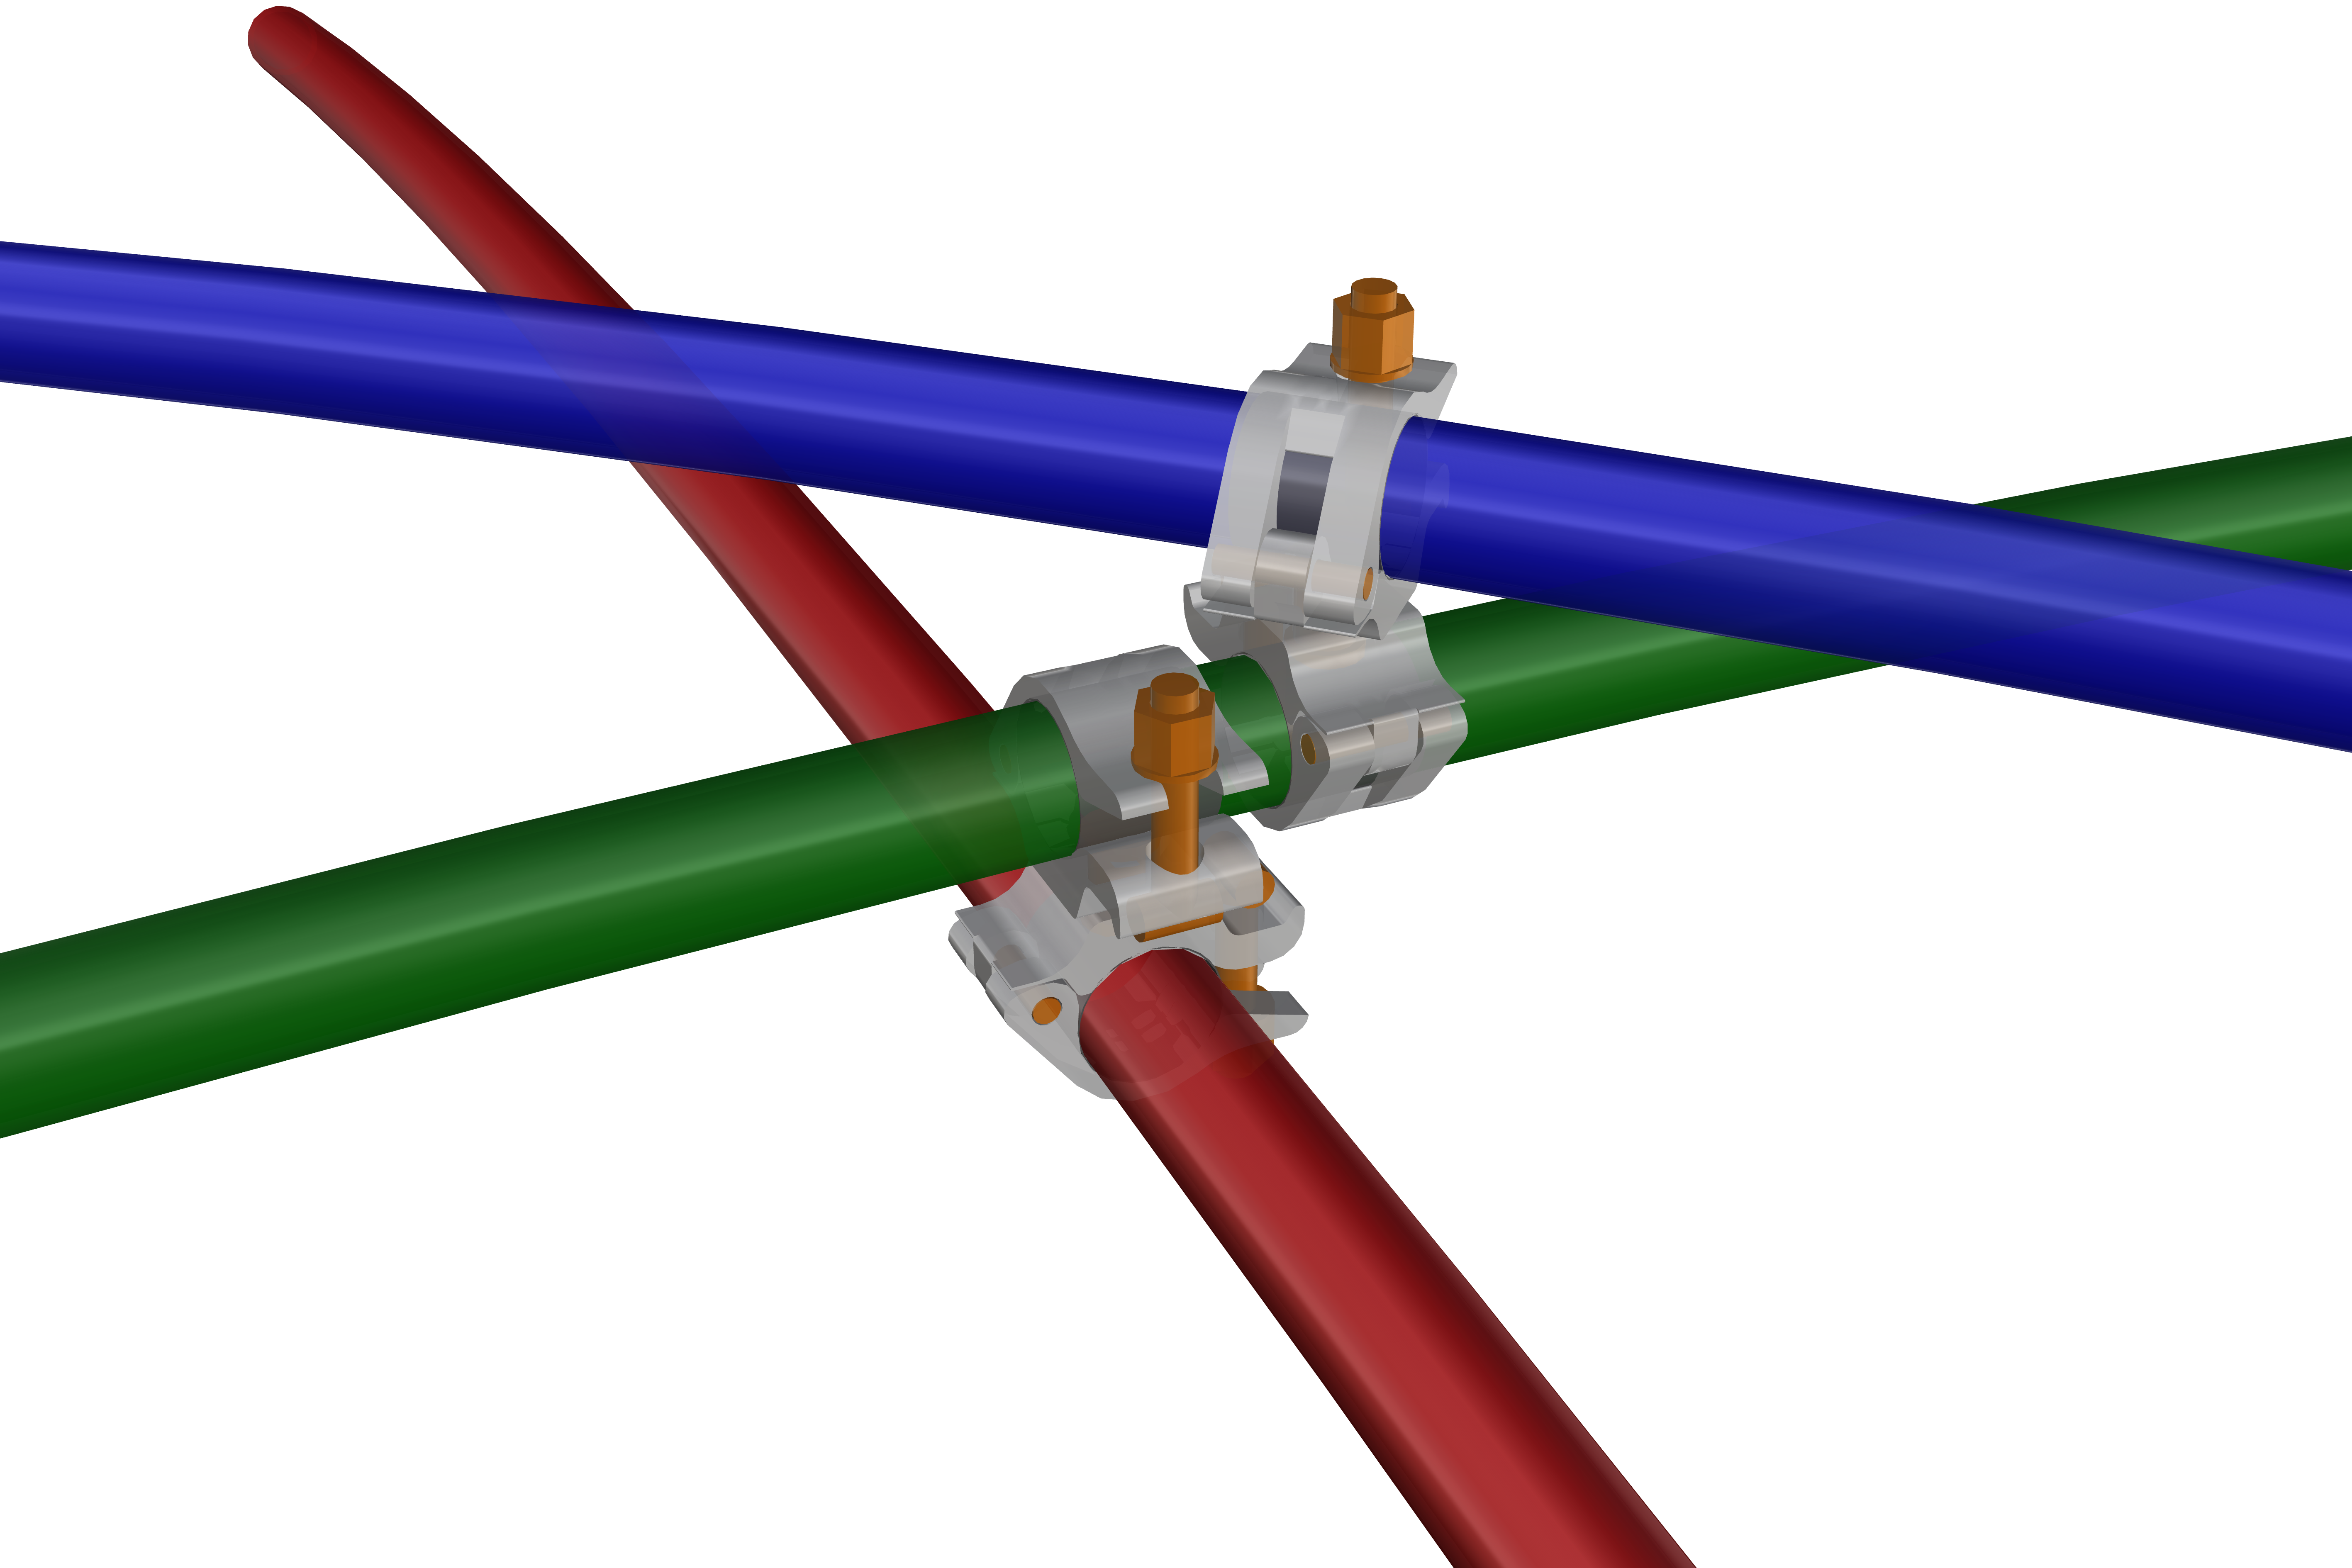
\includegraphics[width=0.48\textwidth]{eccentricity_2.png}\label{fig:eccentricity_b}}
% 		\vspace{0.5cm}
% 		\caption[Reconstruction of the full 3D geometry]{Reconstruction of the full 3D geometry.}
% 		\label{fig:eccentricity}
% 	\end{fullpage}
% \end{figure}
\subsection{Structural analysis}
%------------------------------------------
A full structural analysis is finally performed on the gridshell, using the two mechanical models created previously during the form-finding stage.
The non-braced model is used to check the grid’s behavior during the construction stages. In particular, it must be verified that the primary grid - the one with no triangulation tubes - has no risk of buckling, both for obvious safety reasons and to ensure the accuracy of the final geometry. Indeed, the more the form is likely to buckle, the more it can be triangulated in a buckled geometry different to the targeted geometry. The model with the triangulated grid is used to confirm the gridshell complies with all the structural requirements during its lifetime. Its behavior under standard loadings is evaluated.

% %\newpage \phantom{abc}
% \clearpage
\section{Designing with GFRP materials}\label{sec=design_gfrp}
%------------------------------------------
This section focuses on the GFRP tubes employed for the structure. We present how we managed to deal with this composite material in the eyes of the existing regulatory framework although there is no applicable norms for composite materials (see \cref{sec=codes}). Beyond the administrative strategy, we present how their flexural strength was evaluated (see \cref{sec=flex}) and how the corresponding partial safety factors were detremined (see \cref{sec=safety}).

\subsection{Properties of the tubes}\label{sec=gfrp}
% -------------------------------------------------------
The technical properties of the tube employed for this project are given in \cref{tab:tube}. Although these data were provided by the manufacturer at the time of the project, a test campaign was done to verify the flexural resistance of the tubes taking into account the influence of the swivel couplers clamped on the tubes (see \cref{sec=flex}).
%The characterization of this material is presented in detail in this paper \cite{Kotelnikova2012}.
\blankpage{
	\hbox{}\thispagestyle{empty}
	\AddToShipoutPictureBG*{
		\SBox[%
			node=CAc,
			anchor=center,
			]{%
				\begin{tabular}{@{}l l r @{}}
					\toprule
					Item 							& Standard	 	& Polyester Mat-Roving-Mat \\
					\midrule
					External diameter 				&				& \SI{41.7}{\mm} \\
					Internal diameter 				& 				& \SI{34.7}{\mm} \\
					Wall thickness					& 				& \SI{3.5}{\mm} \\
					Section area					& 				& \SI{4.20e-2}{m^2} \\
					Section moment of inertia			&				& \SI{7.7259e-4}{m^4} \\
					Torsion constant				&				& \SI{15.4518e-4}{m^4} \\
					\midrule
					Shipping length 				& 				& \SI{12.0}{\m} \\
					Glass content by weight 			& ISO 1172		& \SI{60}{\percent}\\
					Specic weight					& ASTM D792		& \SI{1.75}{\kg/m^3}\\
					Linear weight					& 				& \SI{0.735}{\kg/lm}\\
					Coefficient of thermal expansion	& ASTM D696		& \SI{11e-6}{K^{-1}}\\
					\midrule
					Tensile strength					& ASTM D638		& \SI{400}{MPa}\\
					Tensile modulus				& ASTM D638		& \SI{26}{GPa}\\
					Flexural strength				& ASTM D790		& \SI{400}{MPa}\\
					Flexural modulus				& full bending		& \SI{25}{GPa}\\
					Compressive strength			& ASTM D695		& \SI{220}{MPa}\\
					Compressive modulus			& ASTM D695		& \SI{20}{GPa}\\
					\bottomrule
				\end{tabular}
			}
		\PhotoCaptionRef[
			node=CAtl, 
			anchor=north west, 
			% yshift=-\PhotoRefSkip,
			phantom=true,
			]{table}{}{Technical properties of the tube}{tab:tube}
		\PhotoTextBox[
			node=CAbl,
			anchor=south west,
			width=0.6\textwidth,
			border=false,
			]{\tablecaption{tab:tube}}
	}
}

\subsection{Codes for composite materials}\label{sec=codes}
Beyond the technical difficulties related to both design and structural analysis of the shell, the regulatory framework was a vital issue for the success of the project. As it was the first time a structure of this kind was going to host a large number of people for over two years, the question of its reliability over time was a major issue. In order to be built, the gridshell had to comply with existing standards, which do not take into account such an innovative edifice, all in composite material. The strategy adopted to bypass this obstacle is presented herafter.

\subsubsection{First level~: administrative classification of the building}
The first level, administrative, consisted of obtaining from the French authorities an appropriate classification for the building, taking into
consideration the project’s real-time requirement~: a light-weight structure with a short lifespan. As expected, the structure was classified as a \textquote{building open to the public} (EPR in French) from the category \textquote{big tops and tents} (CTS in french) \cite{SiteSecurite}. In this classification, construction procedures and regulations are adapted to the short lifespan of buildings.

\subsubsection{Second level~: compliance with existing standards}
The second level, normative, consisted of ensuring that most of the existing regulatory framework justified the compliance of a structure that would not, at first sight, be considered by standards that do not include composite materials.

As far as possible, the design was made in compliance with the Eurocode, where the structural design is done according to the limit states under normalized loadings (self-weight, snow, wind, etc.). Although, the Eurocodes do not directly take into account composite materials, they propose some probabilistic methods to introduce new materials (EN1990, Annexe D). The mechanical properties of the GFRP pipe were determined as far as possible by tests in conformance with these methods. Alternatively, values were taken according from the Eurocomp \cite{Clarke2003}.\footnote{The Eurocomp is a kind of pre-standard intended for the structural design of buildings and civil engineering works using GFRP composites, consistent with the Eurocode approach. It is considered as the reference design code for GFRP materials.} In some cases, such as for the sleeve, the construction design also benefited from this approach.

\afterpage{%
	\enlargethispage{-6cm}
	\AddToShipoutPictureBG*{% 
		\setlength{\tmpwidth}{(\textwidth-3\PhotoBigSkip)/2}
		\SBox[%
			node=CAbl,
			anchor=south west,
			yshift=2.5cm,
			]{%
				\begin{tabular}{@{}l r r r r r r @{}}
					\toprule
					Connection & $\sigma_1$ & $\sigma_2$ & $\sigma_3$ & $\sigma_4$ & $\sigma_5$ & \tablebf{$\sigma_{k}$} \\
					\midrule
					Without & 456 & 441 & 445 & 460 & 477 & \tablebf{430} \\
					With (20\,Nm) & 444 & 478 & 434 & 479 & 427 & \tablebf{408} \\
					\bottomrule
				\end{tabular}}
		\savenodes{A}
		\SBox[%
			node=CAbr,
			anchor=south east,
			yshift=2.5cm,
			]{%
				\begin{tabular}{@{}l r r @{}}
					\toprule
					Time scale 	& $\gamma$		& $\sigma_{d}$\\
					\midrule
					Short-term 	& $ 2.0$ 			& 200 \\
					Long-term 	& $ 3.0$ 			& 133 \\
					\bottomrule
				\end{tabular}}
		\savenodes{B}
		%%
		\PhotoCaptionRef[
			hrefnode=Atl, 
			node=Abr, 
			anchor=north east,  
			yshift=-\PhotoRefSkip,
		]{table}{}{Flexural tests of the GFRP tubes}{tab:sigma}
		\PhotoCaptionRef[
			hrefnode=Btl, 
			node=Bbr, 
			anchor=north east, 
			yshift=-\PhotoRefSkip,
		]{table}{}{Short-term and long-term values for material resistance}{tab:gamma}
		\PhotoTextBox[
			node=CAbl,
			anchor=south west,
			% yshift=-\PhotoRefSkip,
			width=\textwidth,
			border=false,
			]{%
				\tablecaption{tab:sigma}\par\medskip
				\tablecaption{tab:gamma}\par
				$\gamma$ is the partial coefficient for safety factor. $\sigma_{d}$ is the flexural design strength.
			}
		%%
		% \PhotoCaptionRef[
		% 	hrefnode=Atl,
		% 	node=Atl,
		% 	anchor=south east,
		% 	yshift=\PhotoRefSkip,
		% 	phantom=true,
		% 	]{figure}{}{Reconstruction of the full 3D geometry}{fig:eccentricity}
		% \PhotoCaptionRef[
		% 	hrefnode=Atl,
		% 	node=Atr,
		% 	anchor=north east,
		% 	% yshift=\PhotoRefSkip,
		% 	]{subfigure}{}{Wire frame}{fig:eccentricity_a}
		% \PhotoCaptionRef[
		% 	hrefnode=Btl,
		% 	node=Btr,
		% 	anchor=north east,
		% 	% yshift=\PhotoRefSkip,
		% 	]{subfigure}{}{Full 3D}{fig:eccentricity_b}
		% \intersectnode{CAtl |- Abr}{Pt}
		% \PhotoTextBox[
		% 	node=Pt,
		% 	anchor=north west,
		% 	yshift=-\PhotoSkip,
		% 	width=10cm,
		% 	border=false,
		% 	]{%
		% 		\figurecaption{fig:eccentricity}\par
		% 		\figurecaption{fig:eccentricity_a}\par
		% 		\figurecaption{fig:eccentricity_b}\par
		% 	}
	}
	% \setlength{\tmpheight}{\PhotoHeight}
	% \addtolength{\tmpheight}{4\PhotoBigSkip}
	% \hbox{\vspace{8cm}}
}

\subsection{Flexural strength of the tubes}\label{sec=flex}
%------------------------------------------
The characteristic flexural strength ($\sigma_{k,flex}$) of the GFRP tube was used to verify if the structure complied with the Eurocode. This parameter had a critical impact on the structure’s reliability because in this particular application stresses in the tubes are mainly due to the bending. Thus, it was important to confirm the manufacturer’s permitted value through testing.
Three-point flexural tests were carried out with and without connections (see \cref{plot:gfrp_tubes}) to determine the characteristic strength according to the Eurocode protocol (Annex D)~:
\begin{equation}
\sigma_{k,flex}=\overline{\sigma}(1-k_n\sigma_x)
\end{equation}
For five tests, the factor $k_{n,5\%}$ is 1.80 assuming a normal distribution. It has been proved in \cite{Tayeb2015a} that the connections caused more scattering in the results. Finally, the manufacturer allowed value of \SI{400}{MPa} was confirmed and retained for further calculations.


\blankpage{%
	\AddToShipoutPictureBG*{%
	\Photo[
		node=CAc,
		anchor=center,
		yshift=\plotYadjust,
		]{ch3_creteil/plot/4_gfrp_tube/build.pdf}
	\PhotoCaptionRef[
		node=BL, 
		anchor=north west, 
		yshift=-\PhotoRefSkip,
		phantom=true,
		]{figure}{}{Flexural test of the GFRP tubes}{plot:gfrp_tubes}
	\PhotoTextBox[
		node=CAbl,
		anchor=south west,
		width=10cm,
		border=false,
		]{%
			\figurecaption{plot:gfrp_tubes} (Results from \cite{Tayeb2015a})
		}
	}\hbox{}
}


% \bigskip
% \begin{table}[h]
% 	\centering
% 	\ra{1.1}
%  	\begin{tabular}{@{}l r r r r r r @{}}
% 	\toprule
% 	Connection & $\sigma_1$ & $\sigma_2$ & $\sigma_3$ & $\sigma_4$ & $\sigma_5$ & \tablebf{$\sigma_{k}$} \\
% 	\midrule
% 	Without & 456 & 441 & 445 & 460 & 477 & \tablebf{430} \\
% 	With (20\,Nm) & 444 & 478 & 434 & 479 & 427 & \tablebf{408} \\
% 	\bottomrule
% 	\end{tabular}
% 	\captionof{table}[Flexural tests of the GFRP tubes]{Flexural tests of the GFRP tubes (\SI{}{\mega\pascal}).}
% 	\label{tab:sigma}
% \end{table}

% \begin{figure}[p]
% \centering
% \begin{fullpage}
% 	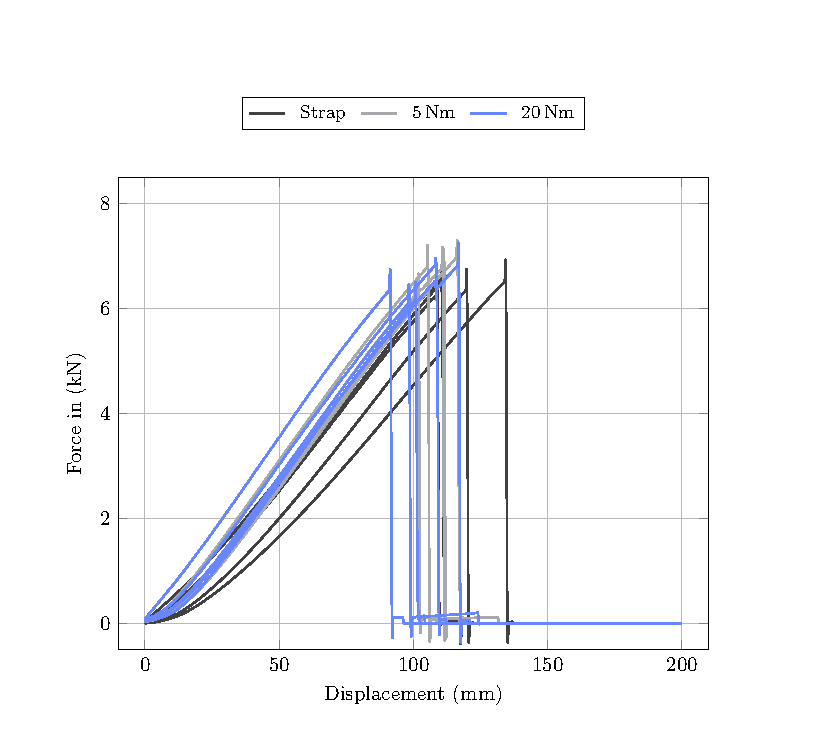
\includegraphics[]{ch3_creteil/plot/4_gfrp_tube/build.pdf}
% 	\caption[Flexural test of the GFRP tubes]{Flexural test of the GFRP tubes. Results from \cite{Tayeb2015a}.}
% 	\label{plot:gfrp_tubes}
% 	%
% 	\vspace{1.5cm}
% 	%
% %	\ra{1.1}
% % 	\begin{tabular}{@{}l r r r r r r @{}}
% %	\toprule
% %	Connection & $\sigma_1$ & $\sigma_2$ & $\sigma_3$ & $\sigma_4$ & $\sigma_5$ & \tablebf{$\sigma_{k}$} \\
% %	\midrule
% %	Without & 456 & 441 & 445 & 460 & 477 & \tablebf{430} \\
% %	With (20\,Nm) & 444 & 478 & 434 & 479 & 427 & \tablebf{408} \\
% %	\bottomrule
% %	\end{tabular}\label{tab:sigma}
% %	\captionof{table}{Three-point flexural tests of the GFRP tubes (\SI{}{\mega\pascal}).}
% 	%
% %	\vspace{1.5cm}
% %	%
% %	 \begin{tabular}{@{}l r r @{}}
% %	\toprule
% %	Time scale 	& $\gamma$		& $\sigma_{d}$\\
% %	\midrule
% %	Short-term 	& $ 2.0$ 			& 200 \\
% %	Long-term 	& $ 3.0$ 			& 133 \\
% %	\bottomrule
% %	\end{tabular}\label{tab:gamma}
% %	\captionof{table}{Short-term and long-term values for material resistance in MPa. $\gamma$ is the partial coefficient for safety factor. $\sigma_{d}$ is the flexural design strength.}
% \end{fullpage}
% \end{figure}


\subsection{Partial safety factors}\label{sec=safety}
%------------------------------------------
The partial coefficients of material resistance (see \cref{tab:gamma}) used in the project were calculated according to the Eurocomp. The short-term coefficient proposed in Eurocomp ($\gamma_{st} = 1.3$) was increased to consider the critical stage of erection, where the deformations could not be controlled accurately.
When dealing with long-term effects in permanently loaded, pultruded composite materials subjected to creeping and relaxation designers should be careful  \cite{Kotelnikova2012,Bank2006}. In this project, this was reflected in the high partial coefficient for long-term effects.

% \blankpage{
% 	\hbox{}\thispagestyle{empty}
% 	\AddToShipoutPictureBG*{%
% 		\SBox[%
% 			node=CAtr,
% 			anchor=north east,
% 			]{%
% 				\begin{tabular}{@{}l r r @{}}
% 					\toprule
% 					Time scale 	& $\gamma$		& $\sigma_{d}$\\
% 					\midrule
% 					Short-term 	& $ 2.0$ 			& 200 \\
% 					Long-term 	& $ 3.0$ 			& 133 \\
% 					\bottomrule
% 				\end{tabular}}
% 				% \captionof{table}[Short-term and long-term values for material resistance]{Short-term and long-term values for material resistance. $\gamma$ is the partial coefficient for safety factor. $\sigma_{d}$ is the flexural design strength.}
% 				% \label{tab:gamma}
% 		\savenodes{A}
% 		\PhotoCaptionRef[
% 			node=Atl, 
% 			anchor=south west, 
% 			yshift=\PhotoRefSkip,
% 		]{table}{}{Short-term and long-term values for material resistance}{tab:gamma}
% 		\PhotoTextBox[
% 			node=CAbl,
% 			anchor=south west,
% 			% yshift=-\PhotoBigSkip-\PhotoSkip,
% 			% width=10cm,
% 			border=false,
% 			]{%
% 				\tablecaption{tab:gamma}\par\medskip
% 				$\gamma$ is the partial coefficient for safety factor. $\sigma_{d}$ is the flexural design strength.
% 			}
% 	}
% }

% \bigskip
% \begin{table}[h]
% \centering
% 	\ra{1.1}
%  	\begin{tabular}{@{}l r r @{}}
% 	\toprule
% 	Time scale 	& $\gamma$		& $\sigma_{d}$\\
% 	\midrule
% 	Short-term 	& $ 2.0$ 			& 200 \\
% 	Long-term 	& $ 3.0$ 			& 133 \\
% 	\bottomrule
% 	\end{tabular}
% 	\caption[Short-term and long-term values for material resistance]{Short-term and long-term values for material resistance. $\gamma$ is the partial coefficient for safety factor. $\sigma_{d}$ is the flexural design strength.}
% 	\label{tab:gamma}
% \end{table}



\pagebreak
\section{Construction details}\label{sec=construction_details}
% ====================
In this project, one can identify 4 major structural details : the swivel coupler for connecting composite tubes to assemble the grid (see \cref{fig:swivel}) ; the steel sleeve for connecting several composite tubes to obtain long members from initially short pieces of tubes (see \cref{fig:sleeve}) ; the ground anchorages for fixing the structure to the concrete slab (see \cref{fig:anchorage}) and the lacing edge beam of the fabric (see \autoref{fig:edge}). The challenging issue of connecting the steel and composite parts was solved similarly for sleeve and anchorage details.

\subsection{The swivel coupler}\label{sec=swivel}
% -------------------------------------------------------
Tubes are connected together with scaffold swivel couplers (see \cref{fig:swivel}). Each connection is composed of two collars (\O\;\SI{42}{\mm} and \SI{38}{\mm} wide) linked by a steel axis (see \cref{fig:swivel_dwg}). Thus the collars can freely rotate around the axis of the connection. This degree of freedom is responsible for the lack of in-plane shear stiffness of the primary grid and this is precisely this mechanism that allows the flat grid to deform into a free form surface. Each collar is itself composed of two hemicylindrical parts so that it can be opened to easily engage a tube. A M12 nut and a swivel T-bolt allow to lock the tube in the collar using friction. Collars are positioned over a \SI{1.5}{\mm} thick epdm ribbon wrapped around the tubes (see \cref{fig:swivel_dwg}). Once clamped in the connection, the tubes are spaced by a \SI{68}{\mm} distance from axis to axis. Although the mechanical consequences of this eccentricity could be neglected to a first-order approximation, this is not the case for the geometric consequences it induces as explained in \cref{sec=asbuilt}.

\afterpage{%
	\AddToShipoutPictureBG*{% 
		\Photo[
			node=CAtl,
			anchor=north west,
			xshift=0mm,
			gopt={width=\textwidth},
			]{swivel.pdf}%
		\savenodes{A}
		\intersectnode{CAtl |- Abr}{Pt}
		\PhotoCaptionRef[
			hrefnode=Atl,
			node=Atr,
			anchor=south east,
			yshift=\PhotoRefSkip,
			phantom=true,
			]{figure}{}{Technical drawing of the swivel coupler}{fig:swivel_dwg}
		\PhotoTextBox[
			node=Abl,
			anchor=north west,
			yshift=-\PhotoSkip,
			width=8cm,
			border=false,
			]{%
				\figurecaption{fig:swivel_dwg}\par\medskip
				GFRP tubes (1, 2, 3). Swivel couplers (5, 8). EPDM layer (6). M12 swivel T-bolt (7). M12 nut (4) and plastic cap (9).
			}
	}
	\setlength{\tmpheight}{\PhotoHeight+\PhotoBigSkip}
	% \addtolength{\tmpheight}{\PhotoBigSkip}
	\hbox{\vspace{\tmpheight}}
}

% \begin{figure}[t]
% 	\centering
% 	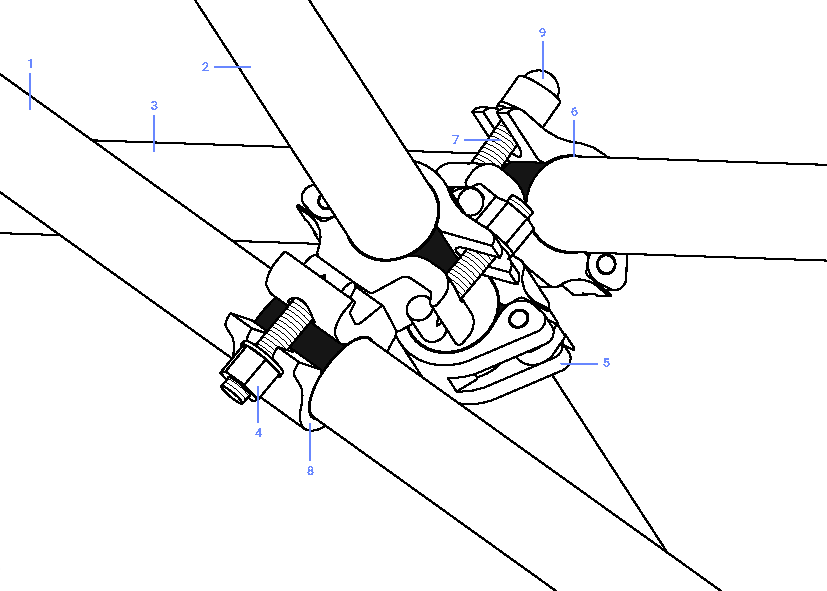
\includegraphics[width=0.8\textwidth]{swivel.pdf}
% 	\caption[Technical drawing of the swivel coupler]{Technical drawing of the swivel coupler. GFRP tubes (1, 2, 3). Swivel couplers (5, 8). EPDM layer (6). M12 swivel T-bolt (7). M12 nut (4) and plastic cap (9).}
% 	\label{fig:swivel_dwg}
% \end{figure}

\subsubsection{Interface layer}
This coupler is made to assemble two scaffold steel tubes together. Workers should tight strongly the collars of the coupler to ensure that the steel tubes won't slide in their collar. Here, it is clearly impossible to do that. Indeed the GFRP tube is too thin (only \SI{3.5}{\mm} thick) and tightening the collars to the maximum would damage it or even make it collapse. However, preventing the connections to slide along the tubes is critical to maintain the in-plane shear degree of freedom of the grid. If connections would slide, the grid would probably not deploy in space as intended, because its deployability relies on the fact that the mesh is equilateral. The grid kinematic would be blocked at some points, developing high stresses that would lead to breakages. To maintain a sufficient level of sliding resistance while preserving the material integrity it was decided to introduce an interface layer to~:
\begin{itemize}
\item Increase the poor friction coefficient between the steel collar and the GFRP tube.
\item Improve the distribution of stresses generated by the transverse compression of the collar over the tube, thus allowing a stronger clamping of the collar.
\end{itemize}


\blankpage{%
	\AddToShipoutPictureBG*{%
	\Photo[
		node=CAc,
		anchor=center,
		yshift=\plotYadjust,
		]{ch3_creteil/plot/1_layer_benchmark/build.pdf}
	\PhotoCaptionRef[
		node=BL, 
		anchor=north west, 
		yshift=-\PhotoRefSkip,
		phantom=true,
		]{figure}{Influence of the interface layer on the sliding resistance}{Influence of the interface layer on the sliding resistance with a torque set to \SI{5}{Nm} (Results from \cite{Tayeb2015a})}{plot:layer_benchmark}
	\PhotoTextBox[
		node=CAbl,
		anchor=south west,
		border=false,
		]{%
			\figurecaption{plot:layer_benchmark}
		}
	}\hbox{}
}

\blankpage{%
	\AddToShipoutPictureBG*{%
	\Photo[
		node=CAc,
		anchor=center,
		yshift=\plotYadjust,
		]{ch3_creteil/plot/3_tightening/build.pdf}
	\PhotoCaptionRef[
		node=BL, 
		anchor=north west, 
		yshift=-\PhotoRefSkip,
		phantom=true,
		]{figure}{Influence of the tightening on the sliding resistance}{Influence of the tightening on the sliding resistance for a \SI{1.5}{\mm} EPDM layer (Results from \cite{Tayeb2015a})}{plot:tightening}
	\PhotoTextBox[
		node=CAbl,
		anchor=south west,
		border=false,
		]{%
			\figurecaption{plot:tightening}
		}
	}\hbox{}
}

\blankpage{%
	\AddToShipoutPictureBG*{%
	\Photo[
		node=CAc,
		anchor=center,
		yshift=\plotYadjust,
		]{ch3_creteil/plot/2_epdm_temperature/build.pdf}
	\PhotoCaptionRef[
		node=BL, 
		anchor=north west, 
		yshift=-\PhotoRefSkip,
		phantom=true,
		]{figure}{Influence of the temperature on the sliding resistance}{Influence of the temperature on the sliding resistance for a \SI{1.5}{\mm} EPDM layer (Results from \cite{Tayeb2015a})}{plot:epdm_temperature}
	\PhotoTextBox[
		node=CAbl,
		anchor=south west,
		border=false,
		]{%
			\figurecaption{plot:epdm_temperature}
		}
	}\hbox{}
}

Several materials were tested in different thickness. Some of the results are presented in \cref{plot:layer_benchmark}. A \SI{1.5}{\mm} thick EPDM ribbon was found to be suitable for the design requirements of the project. This layer improves significantly the sliding resistance from about \SI{300}{\newton} to about \SI{1200}{\newton}. Once the interface layer had been chosen, further tests were conducted to determine the appropriate clamping for the connections. The aim was to maximize the clamping to get the best sliding resistance (see \cref{plot:tightening}) while preserving the  integrity of the tubes. It was found that a tightening torque between \SI{15}{Nm} to \SI{20}{Nm} was the optimal solution \cite{Tayeb2015a}.

Finally, the ribbons were ordered with a double sided tape (DST) face to facilitate their placement on the tubes. The influence of the temperature regarding the presence of the adhesive has been investigated. The results show that after \SI{40}{\celsius} the scotch creeps and a loss of resistance occurs (see \cref{plot:epdm_temperature}). A recent thermal study of the structure has demonstrated that with no cooling system the temperature inside the building could rise up to \SI{70}{\celsius} (see \cref{sec=temperature,plot:T_3,plot:T_4}).


\subsubsection{Benefits and drawbacks}
This connection has the advantage to be available almost every where, to be really cheap and indestructible compare to the GFRP members. However, there are some drawbacks as it is not tailor-made for this application :
\begin{itemize}
\item The weight of this part is \SI{1.16}{\kg}, which is very heavy compare to the lightness of the system. In this project, the weight of the swivel couplers represents one third of the overall weight of the structure. This could easily be reduced with a dedicated design.
\item The actual design is not adapted to resist sliding. This is critical as explained previously. This problem occurred locally during the lifting of the grid and it was a pain to finish the deployment of the structure.
\item  Although the clamping of the collars enhance the resistance to sliding of the couplers, they also activate the ability to transfer some torsion to the tubes. Unfortunately, the tubes are very weak regarding this type of sollicitation (see \cref{tab:tube}). A better design would propose a kinematics that allow the rotation of each collar around the axis of the connection and the axis of the tube.
\item  As the number of connections is quite large, the clamping process should be at the heart of the design. The later has to guarantee that the workers will not damage unintentionally the structural members. If clamping would be found to be the way to go -- which indeed might be a relevant option -- the structural elements will have to be stronger to resist both clamping and torsion.
\end{itemize}

Furthermore, other design criterion should be taken into account such as the fact that the connection must not damage the membrane. This was resolved in the project thanks to plastic caps (see \cref{fig:sleeve_dwg}). It is worthwhile to mention that the problematic of the connection should be treated in symbiosis with the difficult question of the bracing and the covering as it interacts with all the key parts of the system : grid, bracing and membrane. Some propositions to this complex problem were designed and tested during this thesis through the realization of three timber gridshells (see \cref{fig:jpofav,fig:clc2016}) and one hybrid structure (see \cref{fig:booby}). A noticeable design attempt was proposed for the roof of Chiddingstone's orangery \cref{fig:kent}.


% \begin{figure}[p]
% \centering
% \begin{fullpage}
% 	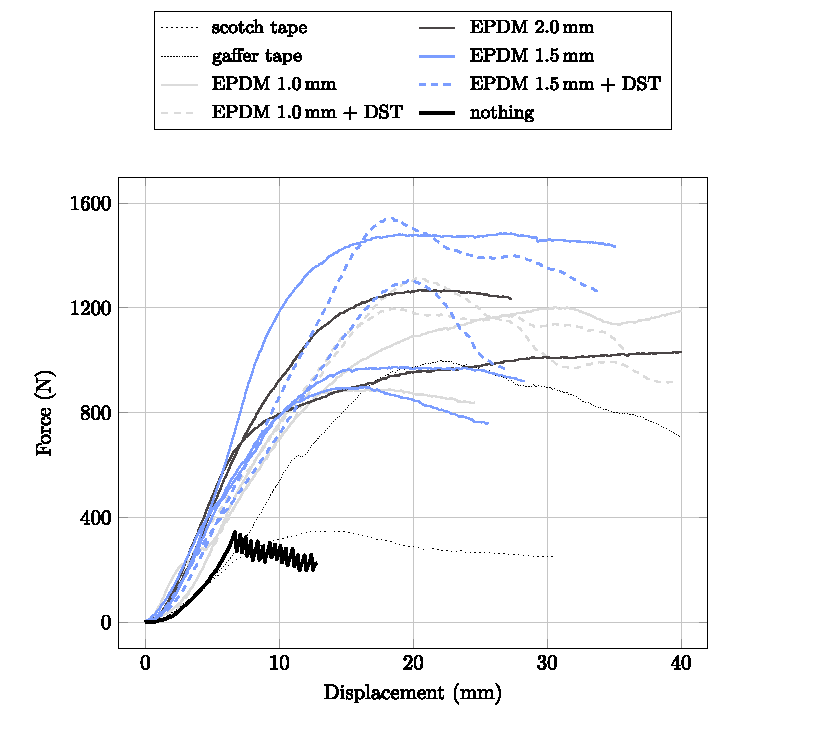
\includegraphics[]{ch3_creteil/plot/1_layer_benchmark/build.pdf}
% 	\caption[Influence of the interface layer on the sliding resistance]{Influence of the interface layer on the sliding resistance (torque set to \SI{5}{Nm}). Results from \cite{Tayeb2015a}.}
% 	\label{plot:layer_benchmark}
% \end{fullpage}
% \end{figure}

% \begin{figure}[p]
% \centering
% \begin{fullpage}
% 	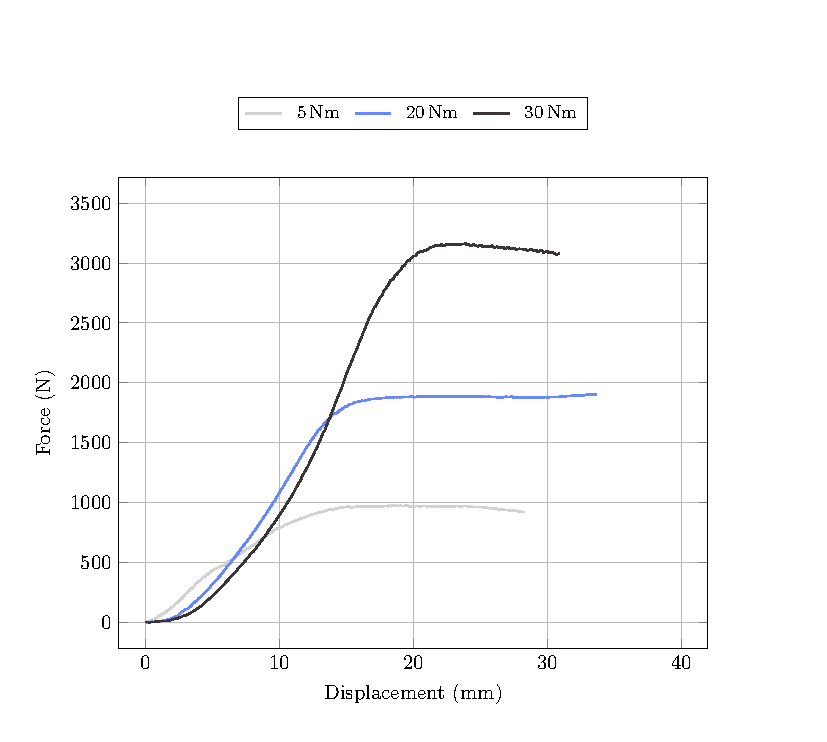
\includegraphics[]{ch3_creteil/plot/3_tightening/build.pdf}
% 	\caption[Influence of the tightening on the sliding resistance]{Influence of the tightening on the sliding resistance for a \SI{1.5}{\mm} EPDM layer. Results from \cite{Tayeb2015a}.}
% 	\label{plot:tightening}
% \end{fullpage}
% \end{figure}

% \begin{figure}[p]
% \centering
% \begin{fullpage}
% 	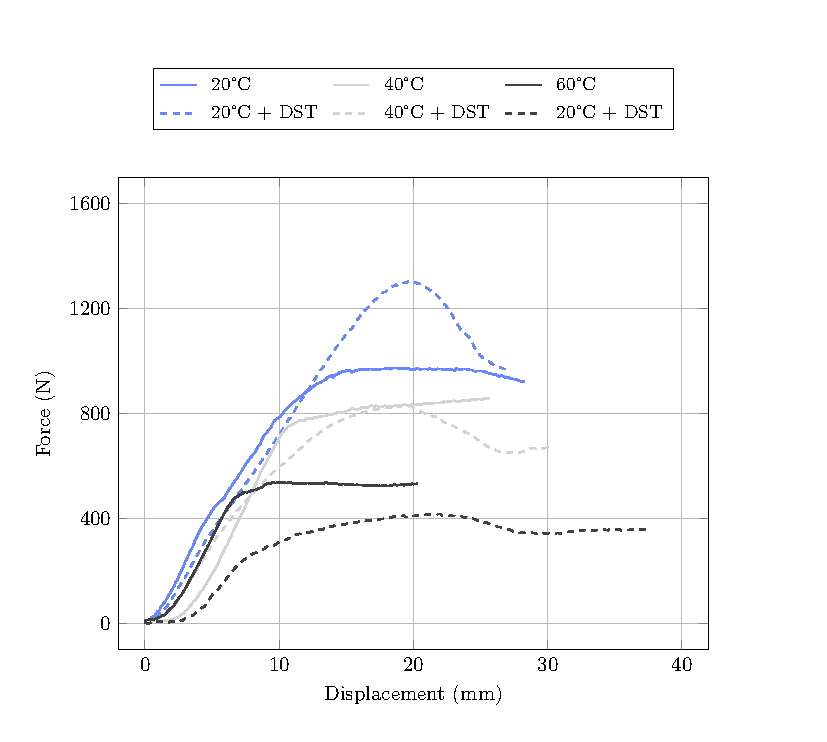
\includegraphics[]{ch3_creteil/plot/2_epdm_temperature/build.pdf}
% 	\caption[Influence of the temperature on the sliding resistance]{Influence of the temperature on the sliding resistance for a \SI{1.5}{\mm} EPDM layer. Results from \cite{Tayeb2015a}.}
% 	\label{plot:epdm_temperature}
% \end{fullpage}
% \end{figure}


\subsection{The sleeve system}
%------------------------------------------

Sleeves are major components in the structural system. The presented design is an important innovation compared with the composite gridshells built previously, where members were simply interrupted or overlapped (see \cref{fig:sleeve_a}). By establishing mechanical and architectural continuities between tubes, the new sleeve system brought the real behavior of the shell closer to its theoretical behavior (see \cref{fig:sleeve_b}).

The sleeve is a steel system that provides mechanical continuity between two adjacent composite tubes for both tension and bending. It is made of three parts~: two connectors linked by a threaded rod (see \cref{fig:sleeve_dwg}). Each connector is a 48.3 × \SI{2.9}{mm} steel tube, slightly larger than the composite tubes it connects, with a welded M20 nut at one end. The connector is pinned to the composite tube with three 10 mm bolts. Some structural adhesive was also employed to fill the gaps and to guarantee good rigidity of the assembly. However, the sleeve is designed to ignore the contribution of the adhesive to the mechanical strength of the system. A M20 threaded rod links the two connectors. It allows tension forces and bending moments to pass from one tube to the other. It does not transfer any torsion.

{%
\enlargethispage{-6cm}
\AddToShipoutPictureBG*{% 
	\Photo[
		node=CAb,
		anchor=south,
		xshift=0mm,
		yshift=2cm,
		gopt={width=\textwidth},
		]{sleeve.pdf}%
	\savenodes{A}
	\intersectnode{CAtl |- Abr}{Pt}
	\PhotoCaptionRef[
		hrefnode=Atl,
		node=Atl,
		anchor=south west,
		yshift=\PhotoRefSkip,
		phantom=true,
		]{figure}{}{Technical drawing of the sleeve system}{fig:sleeve_dwg}
	\PhotoTextBox[
		node=CAbl,
		anchor=south west,
		% yshift=-\PhotoSkip,
		width=10cm,
		border=false,
		]{%
			\figurecaption{fig:sleeve_dwg}
		}
}
}

\blankpage{%
	\thispagestyle{empty}
	\hbox{}
	\AddToShipoutPictureBG*{% 
		\def\tmpwidth{(\textwidth+\ContentOuterMargin+\BleedOuterMargin-\PhotoSkip)/2}
		\Photo[
			node=CAtl,
			anchor=north west,
			xshift=0mm,
			gopt={width=\tmpwidth},
			]{sleeve3.jpg}%
		\savenodes{A}
		\Photo[
			node=Atr,
			anchor=north west,
			xshift=\PhotoSkip,
			gopt={width=\tmpwidth},
			]{sleeve2.jpg}%
		\savenodes{B}
		\Photo[
			node=Abl,
			anchor=north west,
			yshift=-\PhotoBigSkip,
			gopt={width=\tmpwidth},
			]{sleeve5.jpg}%%
		\savenodes{C}
		\Photo[
			node=Bbl,
			anchor=north west,
			yshift=-\PhotoBigSkip,
			gopt={width=\tmpwidth},
			]{sleeve4.jpg}%
		\savenodes{D}
		%%%
		\PhotoCaptionRef[
			node=Atl,
			anchor=south west,
			yshift=-\PhotoSkip,
			phantom=true,
			]{figure}{}{Design and behavior of the the sleeve system}{fig:sleeve_bench}
		\PhotoCaptionRef[
			hrefnode=Atl,
			node=Atl, 
			anchor=south west, 
			yshift=\PhotoRefSkip,
			]{subfigure}{}{Solidays 2011}{fig:sleeve_a}
		\PhotoCaptionRef[
			hrefnode=Btl,
			node=Btl, 
			anchor=south west, 
			yshift=\PhotoRefSkip,
			]{subfigure}{}{Créteil 2013}{fig:sleeve_b}
		\PhotoCaptionRef[
			hrefnode=Ctl,
			node=Cbl, 
			anchor=north west, 
			yshift=-\PhotoRefSkip,
			]{subfigure}{}{Continuity of curvature}{fig:sleeve_c}
		\PhotoCaptionRef[
			hrefnode=Dtl,
			node=Dbl, 
			anchor=north west, 
			yshift=-\PhotoRefSkip,
			]{subfigure}{}{Plastification threshold}{fig:sleeve_d}
		\PhotoTextBox[
			node=CAbl,
			anchor=south west,
			width=10cm,
			border=false,
			]{%
				\figurecaption{fig:sleeve_bench}\par
				\figurecaption{fig:sleeve_a}\par
				\figurecaption{fig:sleeve_b}\par
				\figurecaption{fig:sleeve_c}\par
				\figurecaption{fig:sleeve_d}
			}
	}
}


% \begin{figure}[ht]
% 	\centering
% 	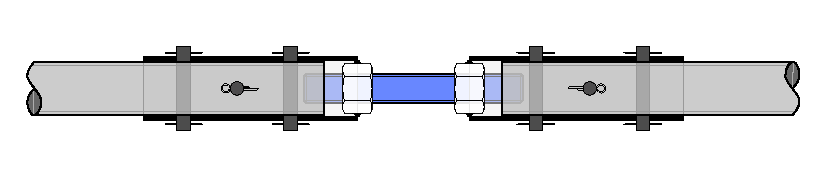
\includegraphics[]{sleeve.pdf}
% 	\caption{Technical drawing of the sleeve system.}
% 	\label{fig:sleeve_dwg}
% \end{figure}

\subsubsection{Mechanical behaviour}

Tension forces are transferred from the composite tube to the connector through shear in the pins. Owing to a lower bearing resistance in the composite than in the steel, each of the three pins could be gradually loaded. When loading the system, initially, only one of the three pins is in contact with both the steel tube and the composite tube, because of inevitable minor manufacturing gaps. When the axial load is increased, this pin starts to “eat” into the composite tube until the second pin also comes in contact. Thus, the axial load is transferred equally between the two pins. This scheme can work with more pins until another failure mode occurs.
For this mode of composite failure, which prevailed in this case, the total bearing capacity of the assembly is thus three times the capacity of a single pin. This total bearing capacity can be calculated from the compressive strength, the composite thickness and the pin diameter~:
\begin{equation}
	F = 3 \times f_{u,c}\cdot d \cdot t = \SI{3150}{daN}
\end{equation}
In the next section, tests carried out at the Navier laboratory to confirm the predicted value are presented.
Bending moments were transferred through the threaded rod of the sleeve. This part was designed to reach the two following qualitative criterions simultaneously~:
\begin{itemize}
\item
Firstly, the bending stiffness of the rod should be roughly equivalent to the composite bending stiffness to preserve the curvature’s continuity along the system  (see \cref{fig:sleeve_c}). This continuity was of prime importance from an architectural point of view.
\begin{equation}
	\frac{EI_{rod}}{EI_{gfrp}} \simeq 1
	\label{eq:r1}
\end{equation}
\item


\afterpage{%
	\AddToShipoutPictureBG*{% 
		\setlength{\tmpwidth}{(\textwidth-\PhotoBigSkip)/2}
		\Photo[
			node=CAt,
			anchor=north east,
			xshift=-\PhotoBigSkip/2,
			gopt={width=\tmpwidth},
			]{pin.jpg}%
		\savenodes{A}
		\Photo[
			node=CAt,
			anchor=north west,
			xshift=\PhotoBigSkip/2,
			gopt={width=\tmpwidth},
			]{pin2.jpg}%
		\savenodes{B}
		%%
		\PhotoCaptionRef[
			hrefnode=Atl,
			node=Atl,
			anchor=south east,
			yshift=\PhotoRefSkip,
			phantom=true,
			]{figure}{}{Typical failure modes when testing the sleeve system in traction}{fig:sleeve_failure}
		\PhotoCaptionRef[
			hrefnode=Atl,
			node=Abr,
			anchor=north east,
			yshift=-\PhotoRefSkip,
			]{subfigure}{}{Tearing}{fig:sleeve_e}
		\PhotoCaptionRef[
			hrefnode=Btl,
			node=Bbr,
			anchor=north east,
			yshift=-\PhotoRefSkip,
			]{subfigure}{}{Contact compression}{fig:sleeve_f}
		\intersectnode{CAtl |- Abr}{Pt}
		\PhotoTextBox[
			node=Pt,
			anchor=north west,
			yshift=-2\PhotoBigSkip,
			width=10cm,
			border=false,
			]{%
				\figurecaption{fig:sleeve_failure}\par
				\figurecaption{fig:sleeve_e}\par
				\figurecaption{fig:sleeve_f}
			}
	}
	\hbox{\vspace{8cm}}
}

Secondly, the steel quality of the rod should be adjusted such that plastification begins when the composite tube tends to approach its maximum design stress (a third of the yield stress). Thus the rod acts as a \textquote{fuse}~: if the curvature of the system reaches the maximum allowed curvature, the steel rod starts their plastification. The plastic hinge accumulates the rotation and prevents the curvature to increase in the composite tubes (see \cref{fig:sleeve_d}).
\begin{equation}
	\frac{\raisebox{0.2ex}M^{elastic\,max}_{rod}}{\raisebox{-0.2ex}M^{\sigma = \SI{133}{MPa}}_{gfrp}} \simeq 1
	\label{eq:r2}
\end{equation}
\end{itemize}
In this project, the numerical values for the ratios in \cref{eq:r1,eq:r2} were 0.79 and 0.96 respectively.


\subsubsection{Testing the load-bearing capacity of the pinned connection}
Tensile test of a three-pin connection between a connector and the corresponding composite tube were done (see \cref{plot:pintest}). The graph reflects the elastic behavior of the composite tube up to \SI{35}{kN}, with slight deviations corresponding to the rearrangement of the pins. The compressive stress applied by each pin to the composite tube exceeds its compressive strength. Progressively, the pins are pulled through the tube under a residual force that tends to stabilize at around \SI{20}{kN}. The tests exhibit a ductile behavior of the assembly, which is advantageous for such a structural application.


\doubleblankpage{%
	\hbox{}\thispagestyle{empty}
	\AddToShipoutPictureBG*{% 
	\setlength{\tmpwidth}{(\textwidth-2\PhotoSkip)/3}
	\intersectnode{CAtl |- CAc}{Pt}
	\Photo[
		node=Pt,
		anchor=south west,
		yshift=\PhotoBigSkip/2 + 2.6mm,
		gopt={width=\tmpwidth},
		]{breaking_1}%
	\savenodes{A}
	\Photo[
		node=Abr,
		anchor=south west,
		xshift=\PhotoBigSkip,
		gopt={width=\tmpwidth},
		]{breaking_2}%
	\savenodes{B}
	\Photo[
		node=Bbr,
		anchor=south west,
		xshift=\PhotoBigSkip,
		gopt={width=\tmpwidth},
		]{breaking_3}%
	\savenodes{C}
	%%
	\Photo[
		node=Abl,
		anchor=north west,
		yshift=-\PhotoBigSkip,
		gopt={width=\tmpwidth},
		]{breaking_4}%
	\savenodes{D}
	\Photo[
		node=Dbr,
		anchor=south west,
		xshift=\PhotoBigSkip,
		gopt={width=\tmpwidth},
		]{breaking_5}%
	\savenodes{E}
	\Photo[
		node=Ebr,
		anchor=south west,
		xshift=\PhotoBigSkip,
		gopt={width=\tmpwidth},
		]{breaking_6}%
	\savenodes{F}
	%%
	\PhotoCaptionRef[
		hrefnode=Atl,
		node=Atl,
		anchor=south west,
		yshift=\PhotoRefSkip,
		phantom=true,
		]{figure}{Typical failure modes of a bolt in a pultruded element}{Typical failure modes of a bolt in a pultruded element (\SI{0}{\degree}) \cite{Clarke2003}}{fig:breaking}
	\PhotoCaptionRef[
		hrefnode=Atl,
		node=At,
		anchor=north,
		yshift=-\PhotoRefSkip,
		]{subfigure}{}{Geometry}{fig:breaking_1}
	\PhotoCaptionRef[
		hrefnode=Btl,
		node=Bt,
		anchor=north,
		yshift=-\PhotoRefSkip,
		]{subfigure}{}{Fibres}{fig:breaking_2}
	\PhotoCaptionRef[
		hrefnode=Ctl,
		node=Ct,
		anchor=north,
		yshift=-\PhotoRefSkip,
		]{subfigure}{}{Cleavage}{fig:breaking_3}
	\PhotoCaptionRef[
		hrefnode=Dtl,
		node=Dt,
		anchor=north,
		yshift=-\PhotoRefSkip,
		]{subfigure}{}{Tearing}{fig:breaking_4}
	\PhotoCaptionRef[
		hrefnode=Etl,
		node=Et,
		anchor=north,
		yshift=-\PhotoRefSkip,
		]{subfigure}{}{Inclined compression}{fig:breaking_5}
	\PhotoCaptionRef[
		hrefnode=Ftl,
		node=Ft,
		anchor=north,
		yshift=-\PhotoRefSkip,
		]{subfigure}{}{Contact compression}{fig:breaking_6}
	\PhotoTextBox[
		node=CAbl,
		anchor=south west,
		width=\textwidth,
		border=false,
		]{%
			\figurecaption{fig:breaking}\par\medskip
			\figurecaption{fig:breaking_1}\par
			\figurecaption{fig:breaking_2}\par
			\figurecaption{fig:breaking_3}
		}
	\PhotoTextBox[
		node=CAbl,
		anchor=south west,
		width=\textwidth,
		xshift=3cm,
		border=false,
		]{%
			\figurecaption{fig:breaking_4}\par
			\figurecaption{fig:breaking_5}\par
			\figurecaption{fig:breaking_6}
		}
	}
}{
	\hbox{}\thispagestyle{empty}
	\AddToShipoutPictureBG*{%
	\Photo[
		node=CAc,
		anchor=center,
		yshift=\plotYadjust,
		]{ch3_creteil/plot/6_pin/build.pdf}%
	\PhotoCaptionRef[
		node=BL, 
		anchor=north west, 
		yshift=-\PhotoRefSkip,
		phantom=true,
		phantom=true,
		]{figure}{Tensile test of the pinned connection}{Tensile test of the pinned connection (Results from \cite{Tayeb2015a})}{plot:pintest}
	\intersectnode{CAtl |- Abr}{Pt}
	\PhotoTextBox[
		node=CAbl,
		anchor=south west,
		border=false,
		]{%
			\figurecaption{plot:pintest}
		}
	}
}

% \subfloat[][Geometry]{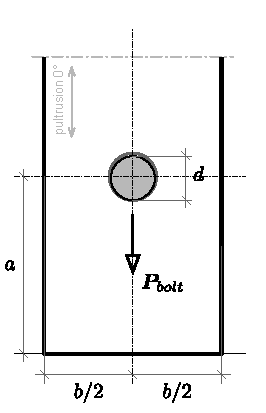
\includegraphics[]{breaking_1}\label{fig:breaking_1}}
% 		\subfloat[][Fibres]{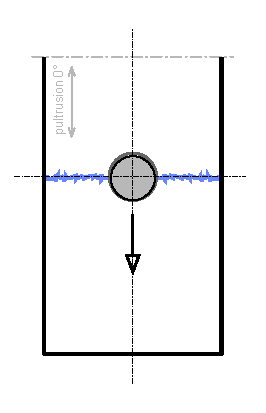
\includegraphics[]{breaking_2}\label{fig:breaking_2}}
% 		\subfloat[][Cleavage]{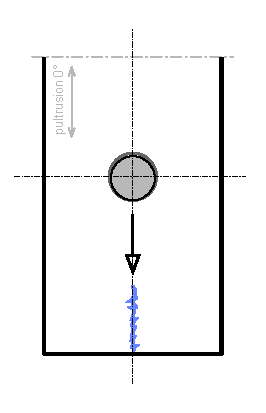
\includegraphics[]{breaking_3}\label{fig:breaking_3}} \\
% 		%
% 		\subfloat[][Tearing]{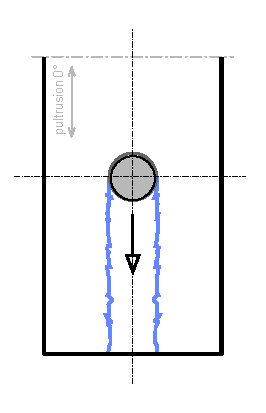
\includegraphics[]{breaking_4}\label{fig:breaking_4}}
% 		\subfloat[][Inclined compression]{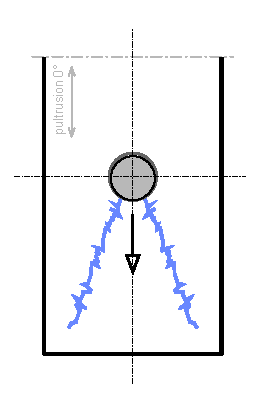
\includegraphics[]{breaking_5}\label{fig:breaking_5}}
% 		\subfloat[][Contact compression]{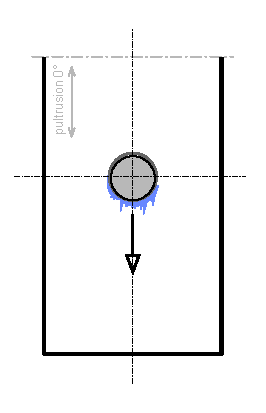
\includegraphics[]{breaking_6}\label{fig:breaking_6}}
% 		%
% 		\vspace{10pt}
% 		\caption[Typical failure modes of a bolt in a pultruded element ]{Typical failure modes of a bolt in a pultruded element (\SI{0}{\degree}) \cite{Clarke2003}.}
% 		\label{fig:breaking}

The theoretical failure modes of a bolt in a pultruded profile are given in \cite{Fiberline2003} and are illustrated in \cref{fig:breaking}. For the present design of the sleeve system, the observed failure modes were tearing (see \cref{fig:sleeve_e}) and contact compression (see \cref{fig:sleeve_f}). Note that this last failure mode is necessary to cumulate the load bearing capacity of each pin.


% \begin{figure}[p]
% 	\centering
% 	\begin{fullpage}
% 	\subfloat[][Solidays 2011]{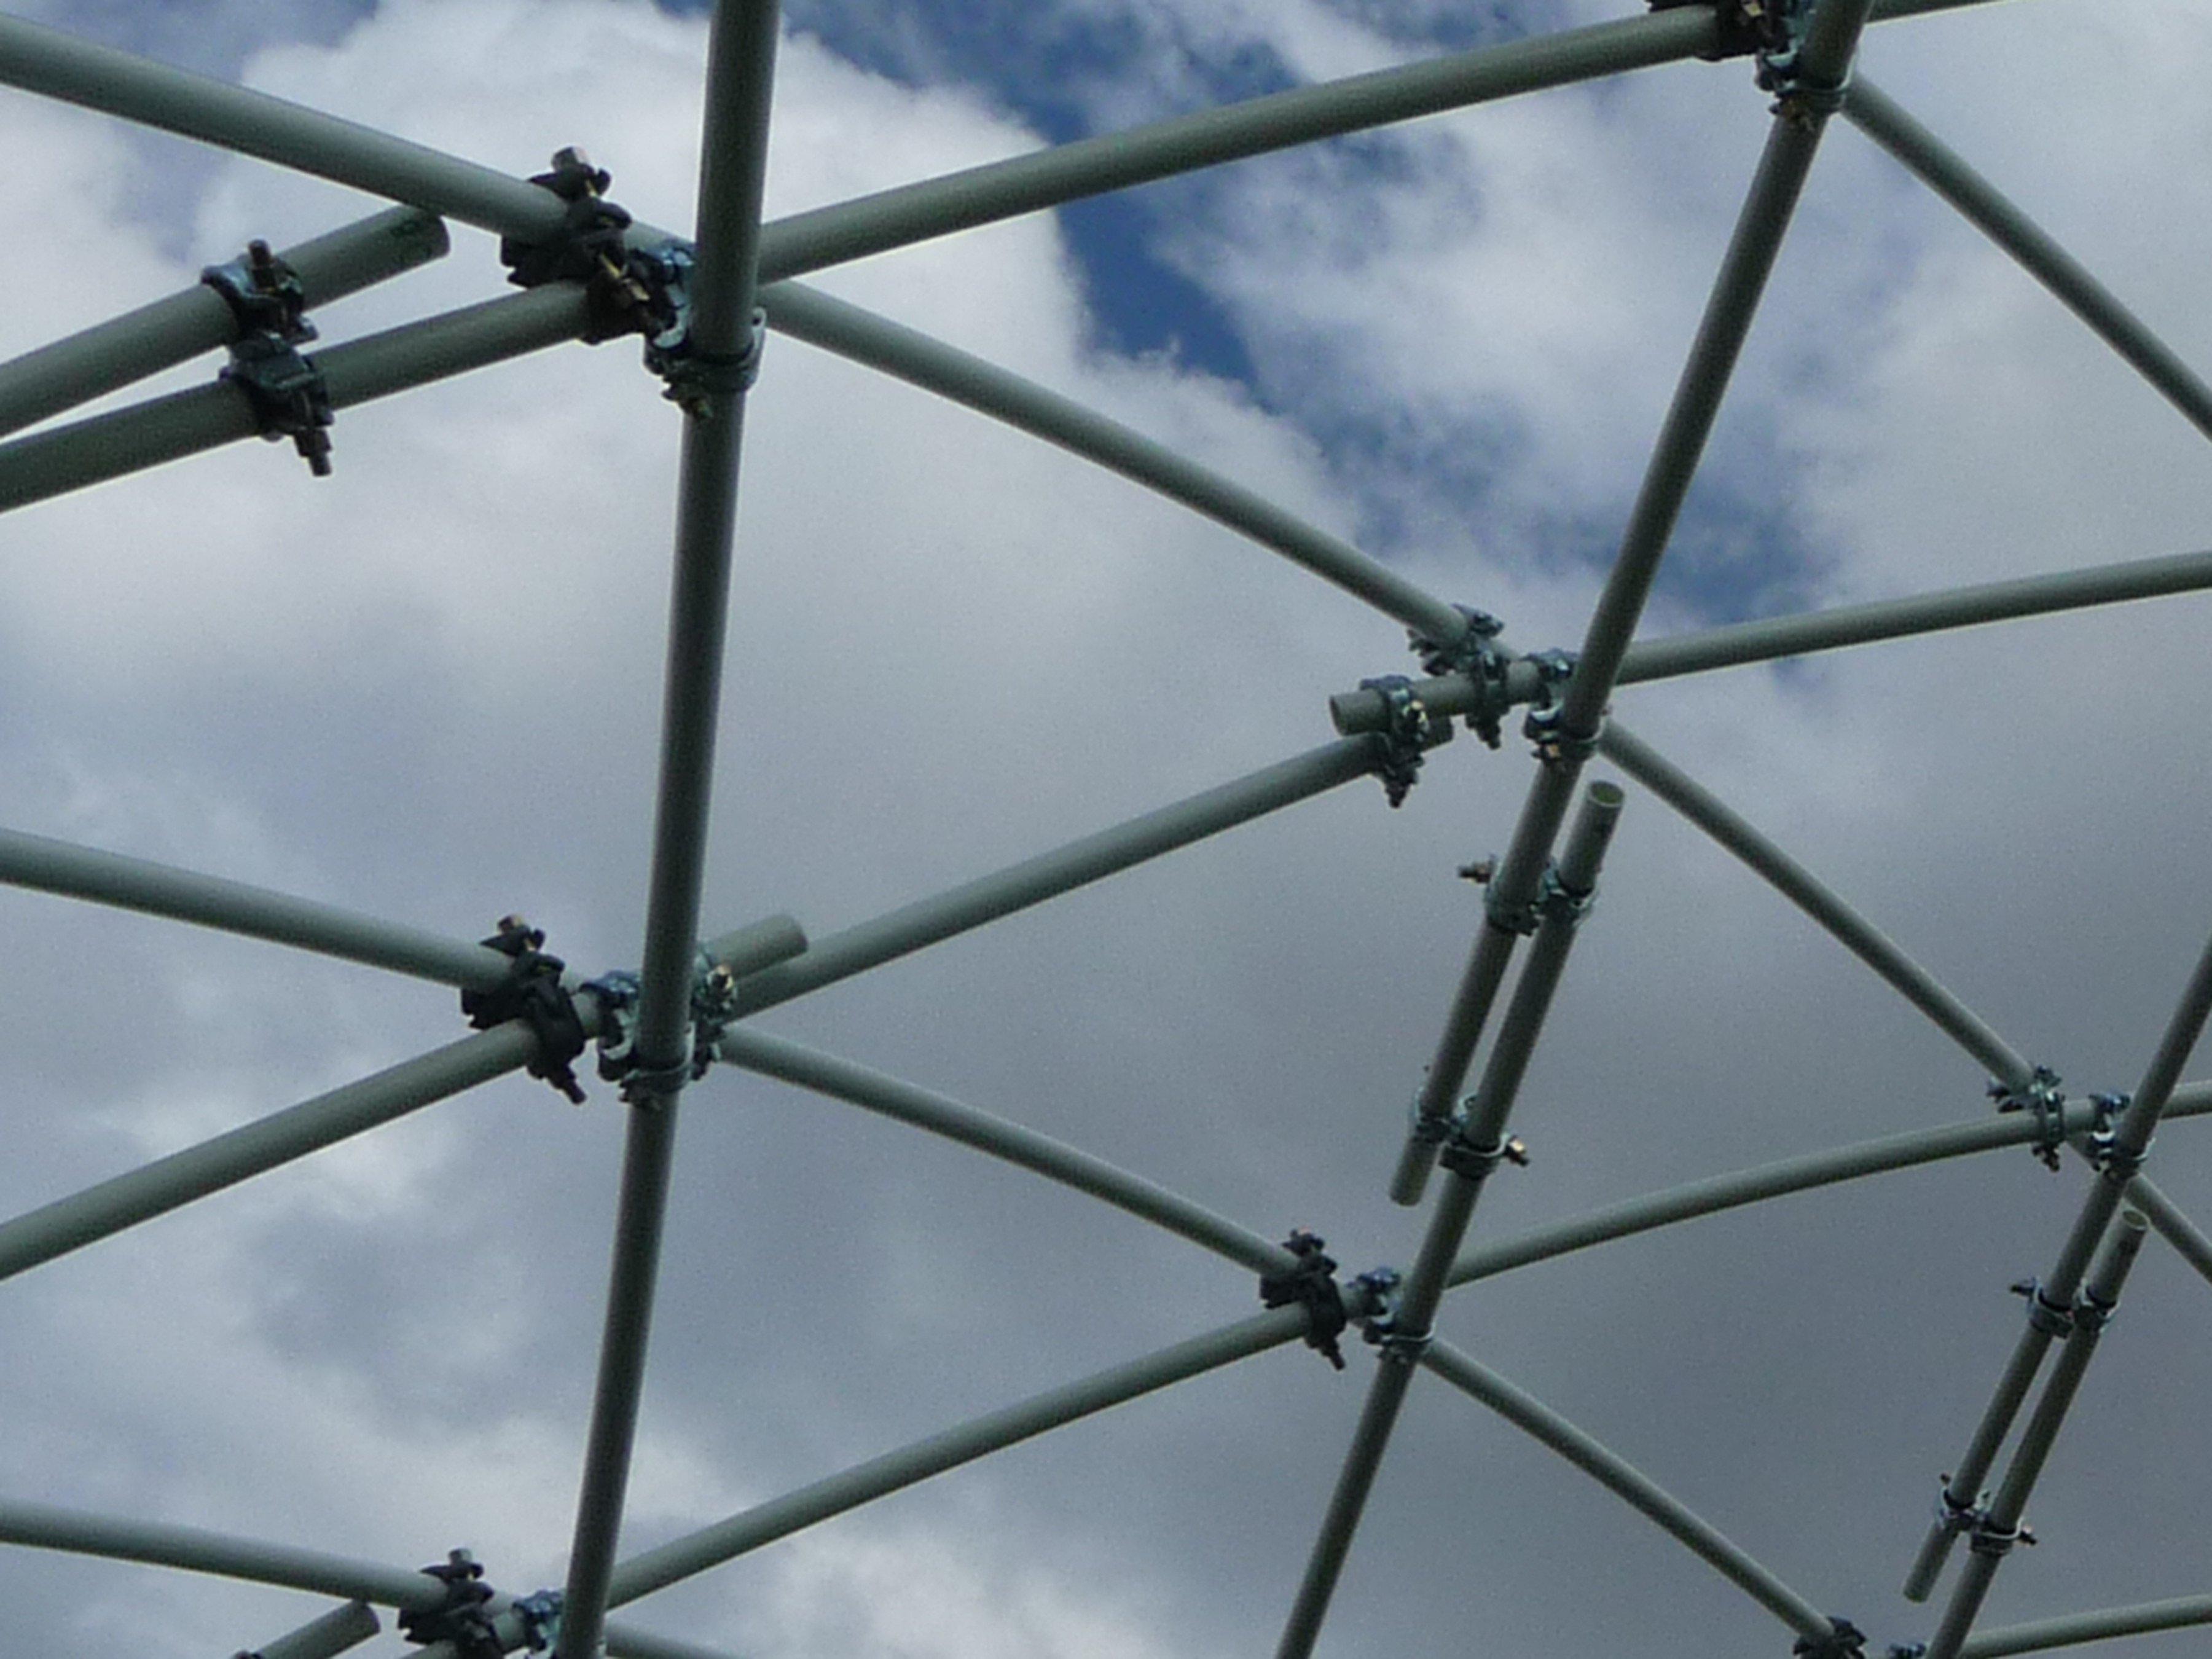
\includegraphics[width=0.48\textwidth]{sleeve3.jpg}\label{fig:sleeve_a}}
% 	\hspace*{\fill}
% 	\subfloat[][Créteil 2013]{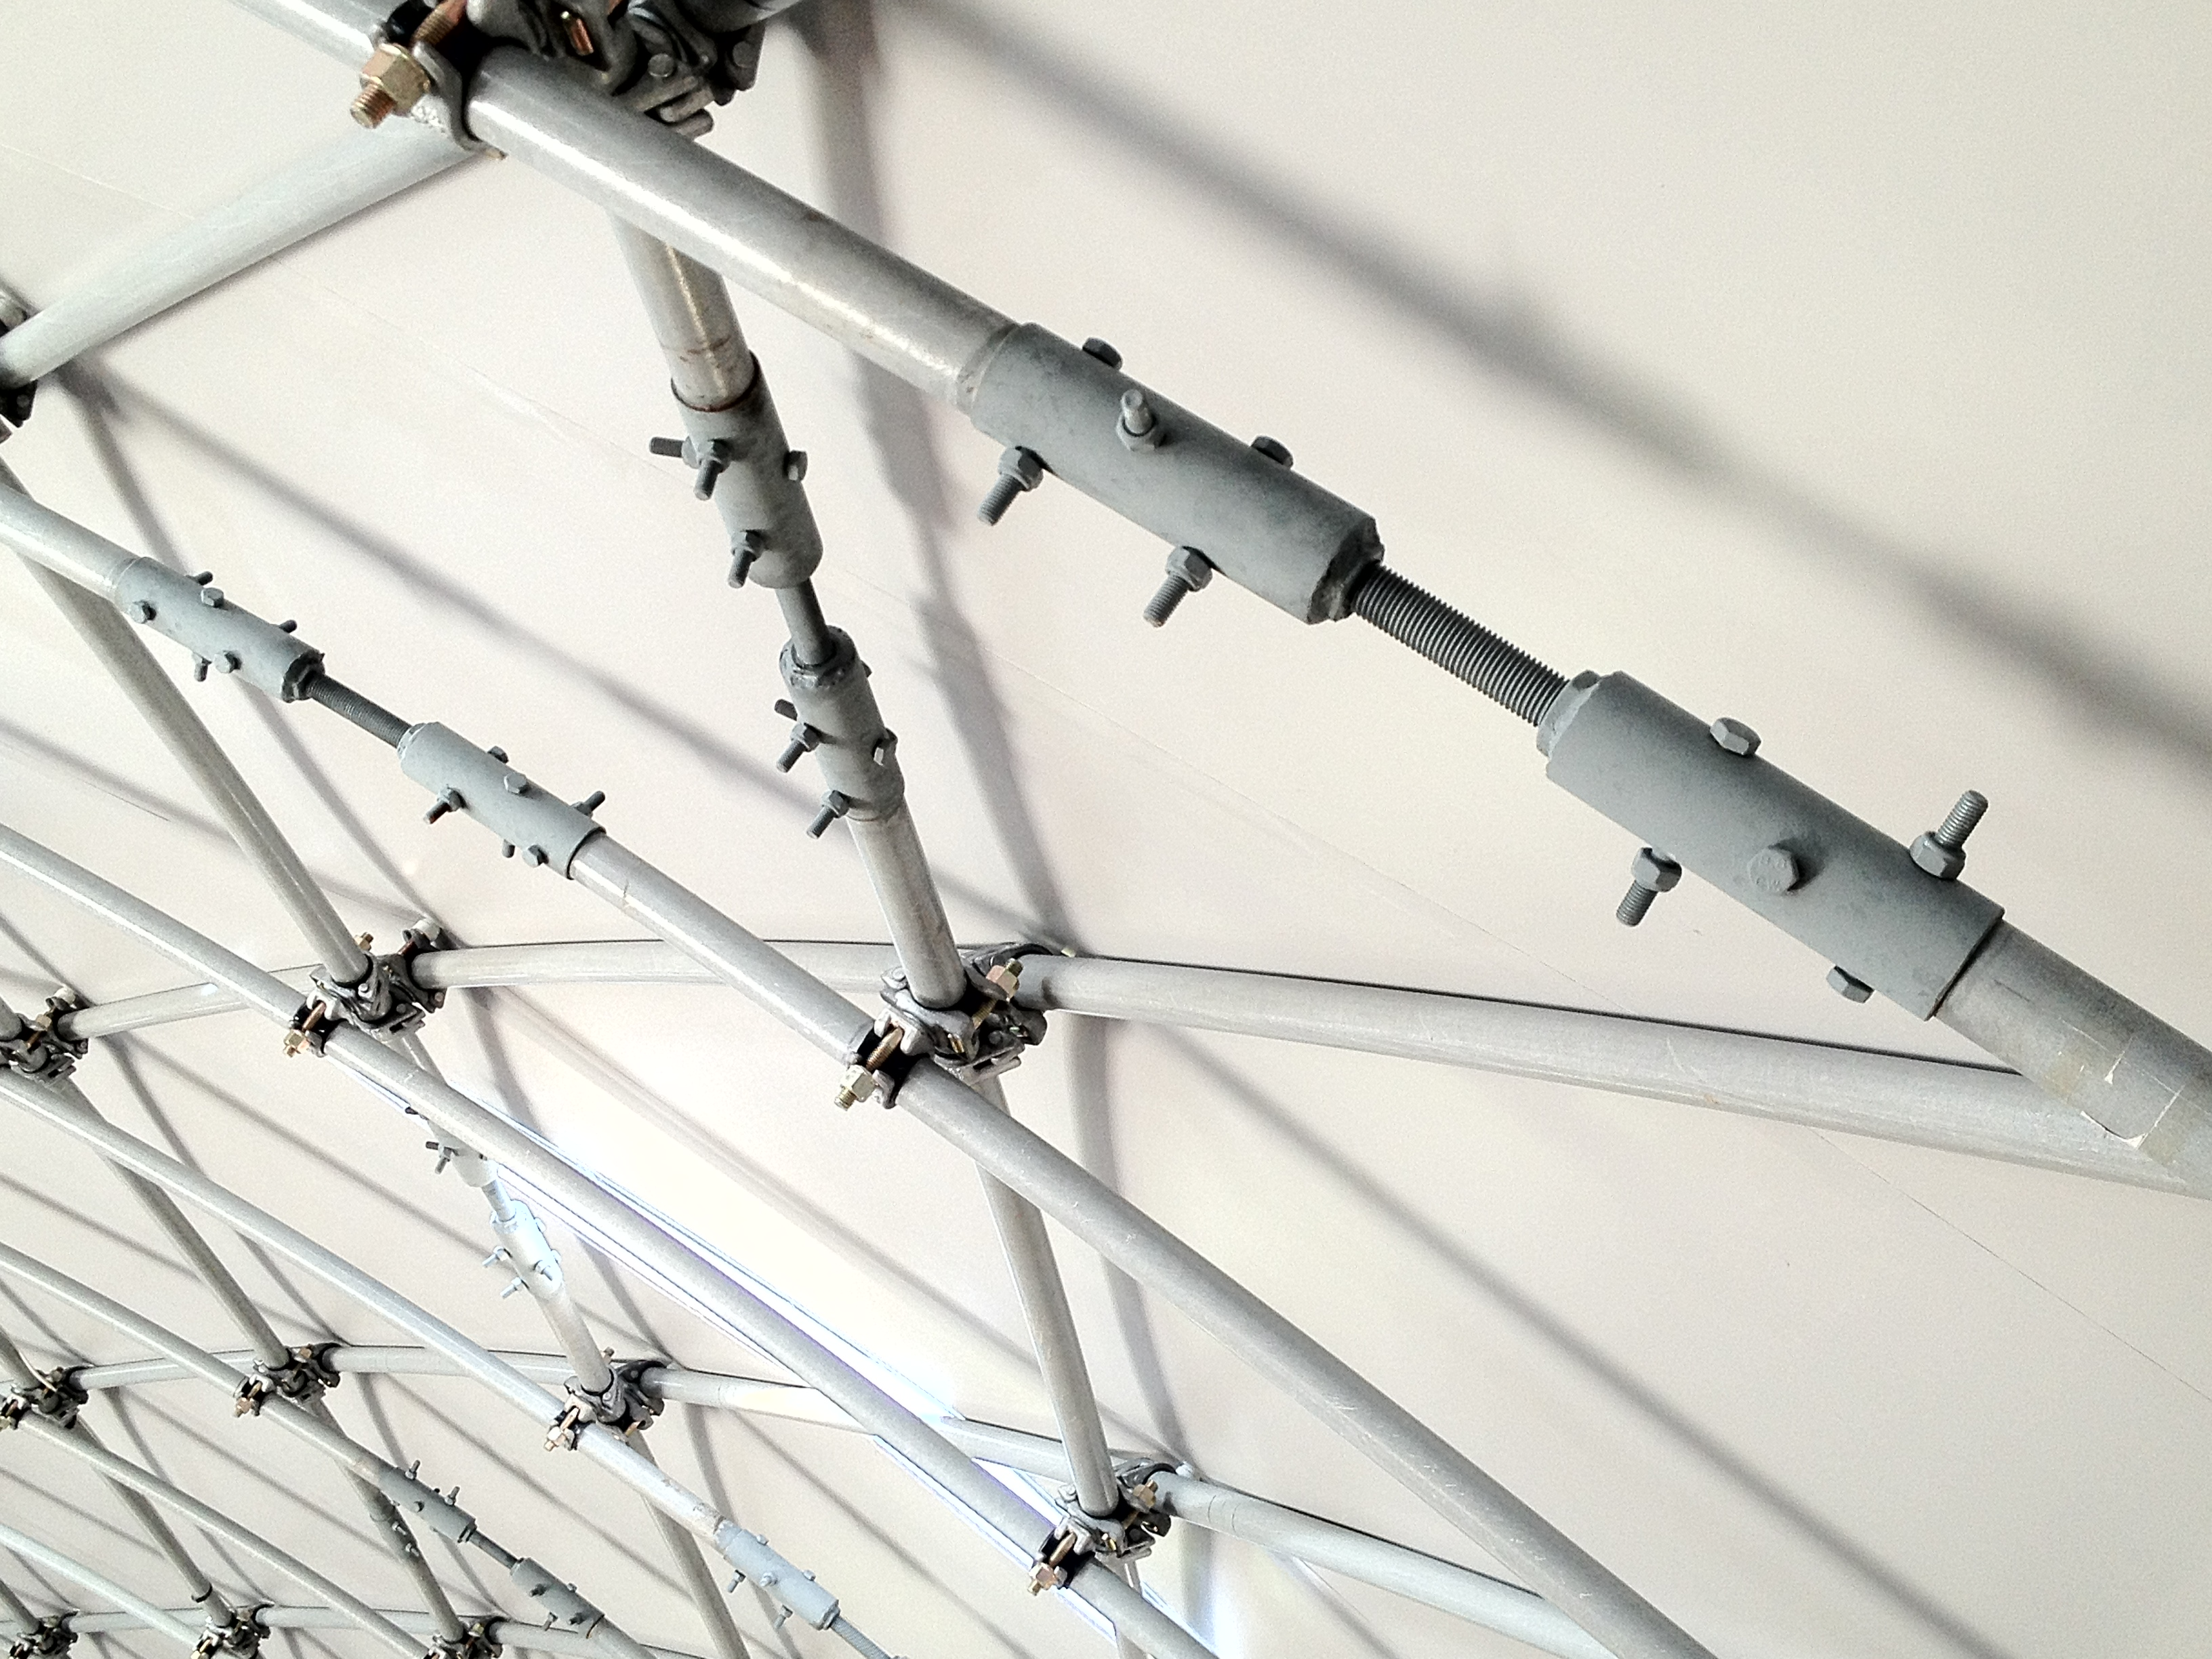
\includegraphics[width=0.48\textwidth]{sleeve2.jpg}\label{fig:sleeve_b}}\\
% 	\subfloat[][Continuity of curvature]{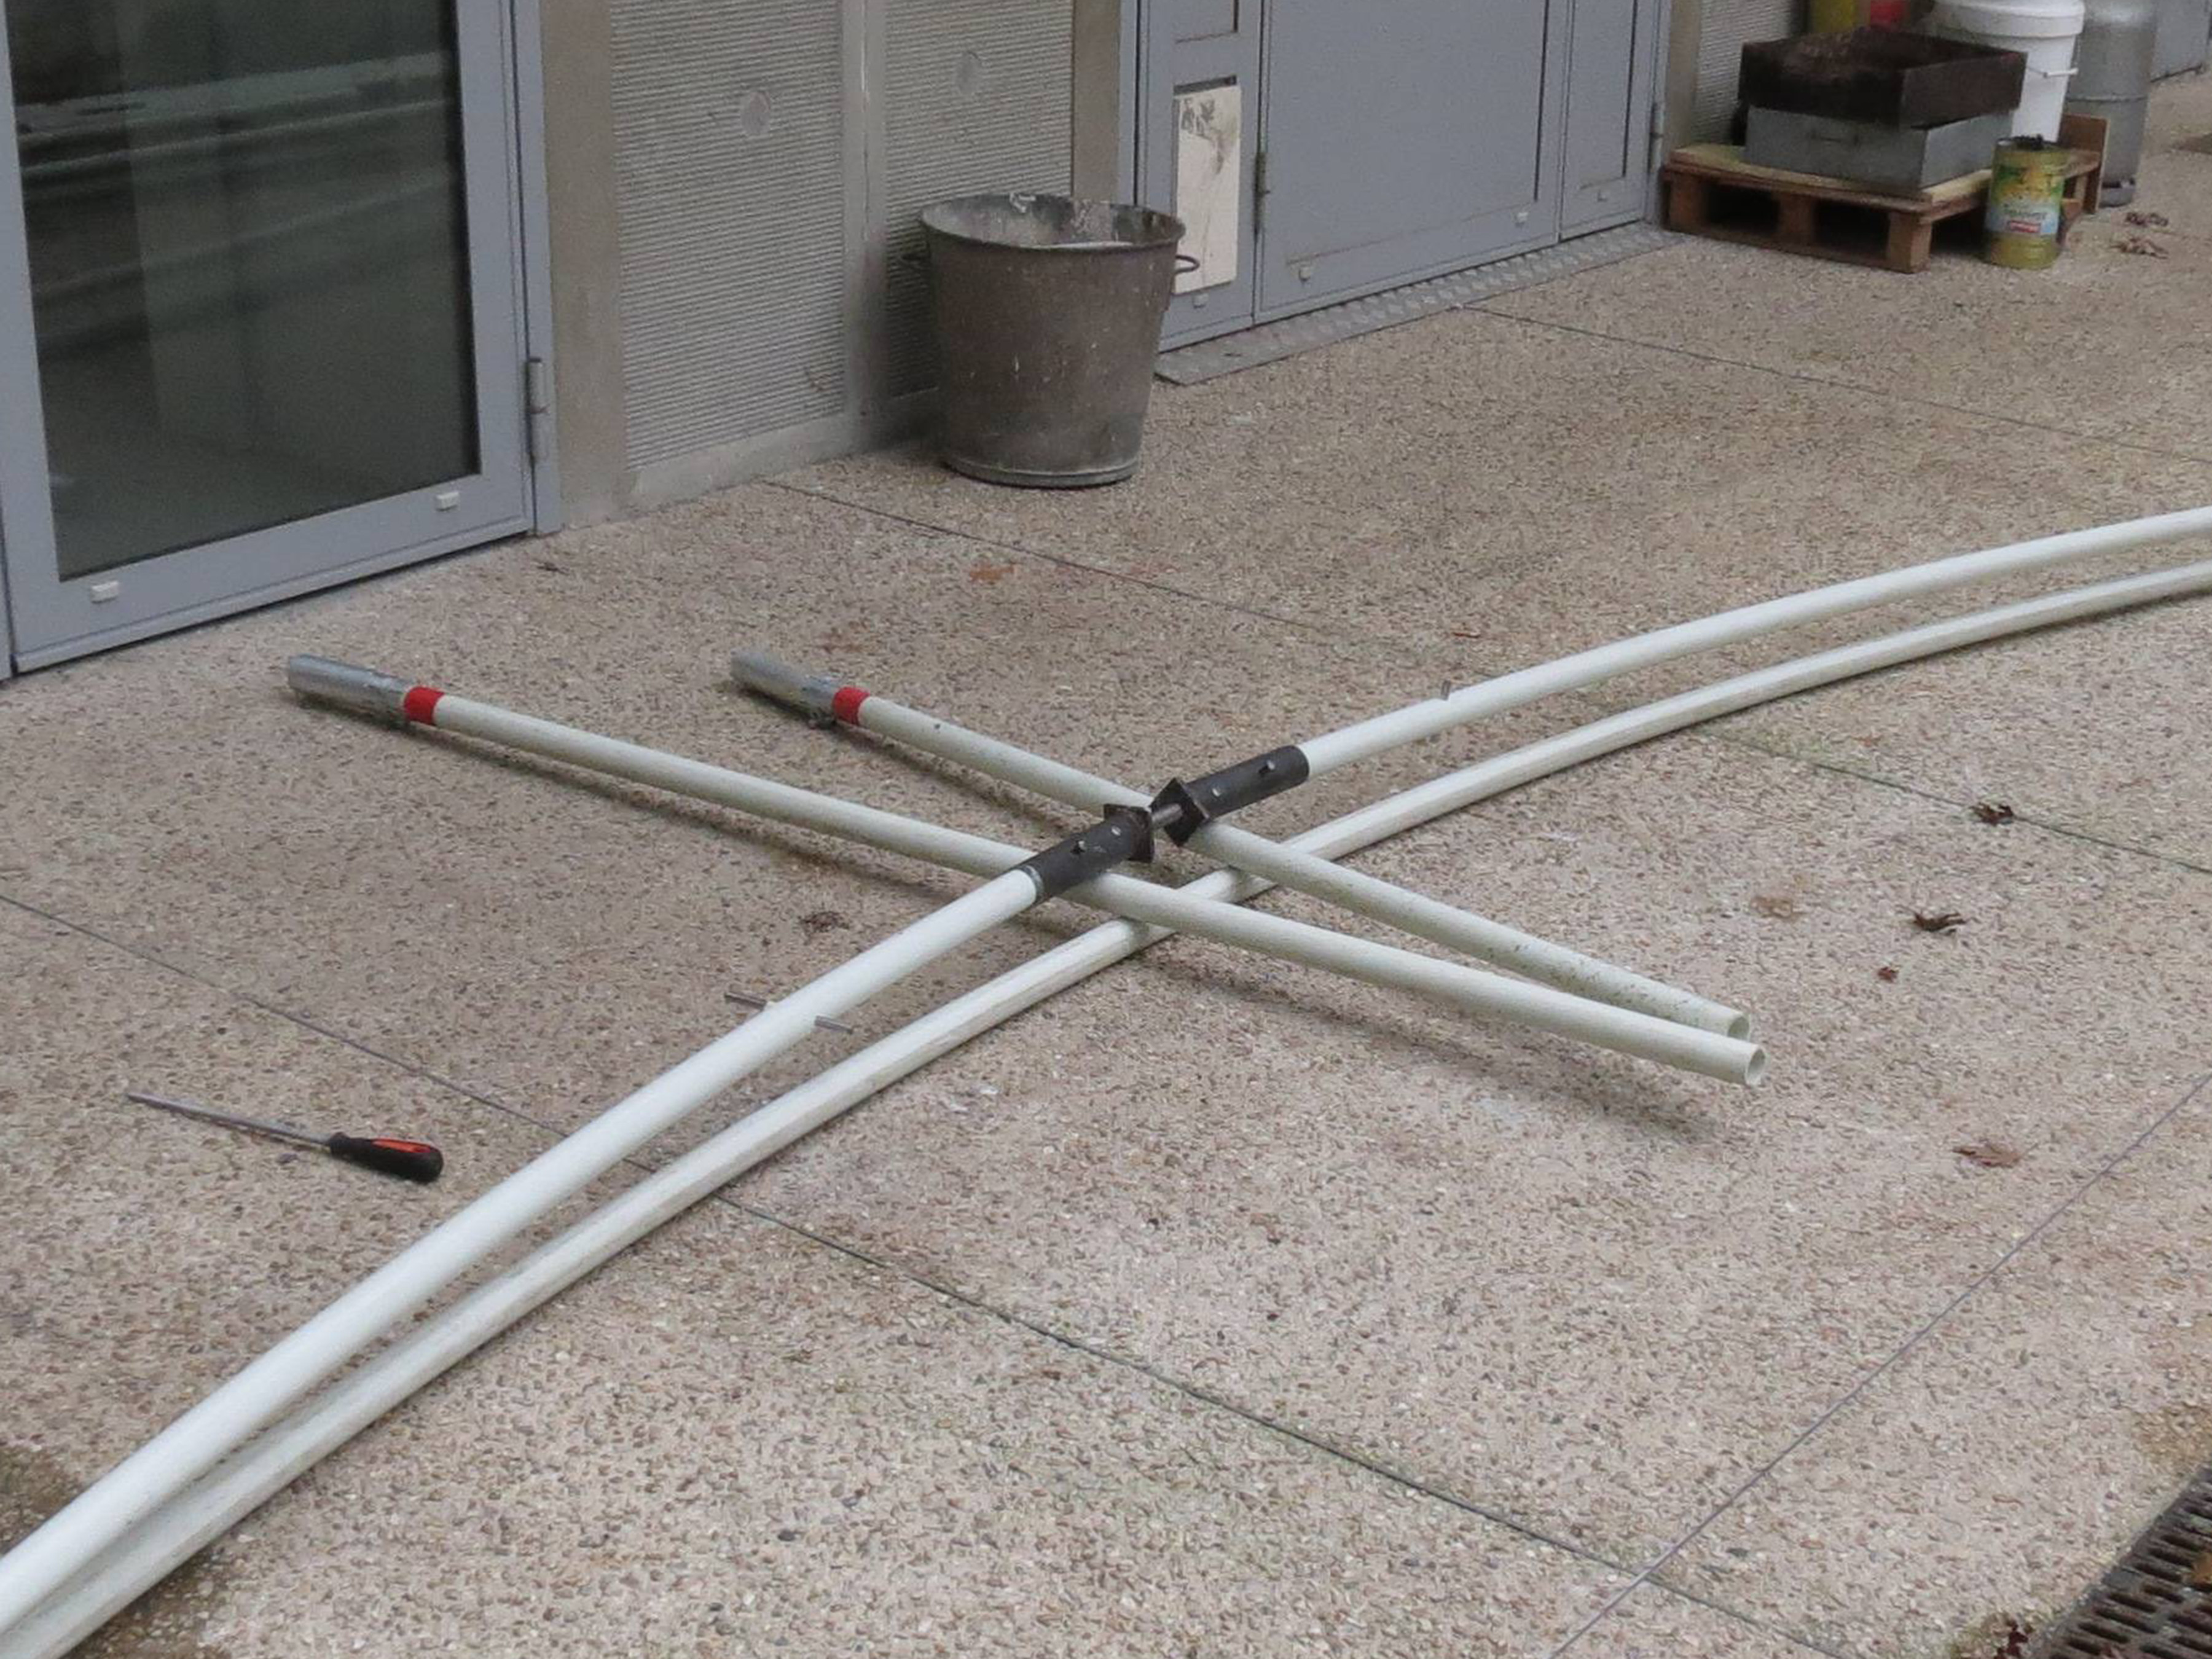
\includegraphics[width=0.48\textwidth]{sleeve5.jpg}\label{fig:sleeve_c}}
% 	\hspace*{\fill}
% 	\subfloat[][Plastification threshold]{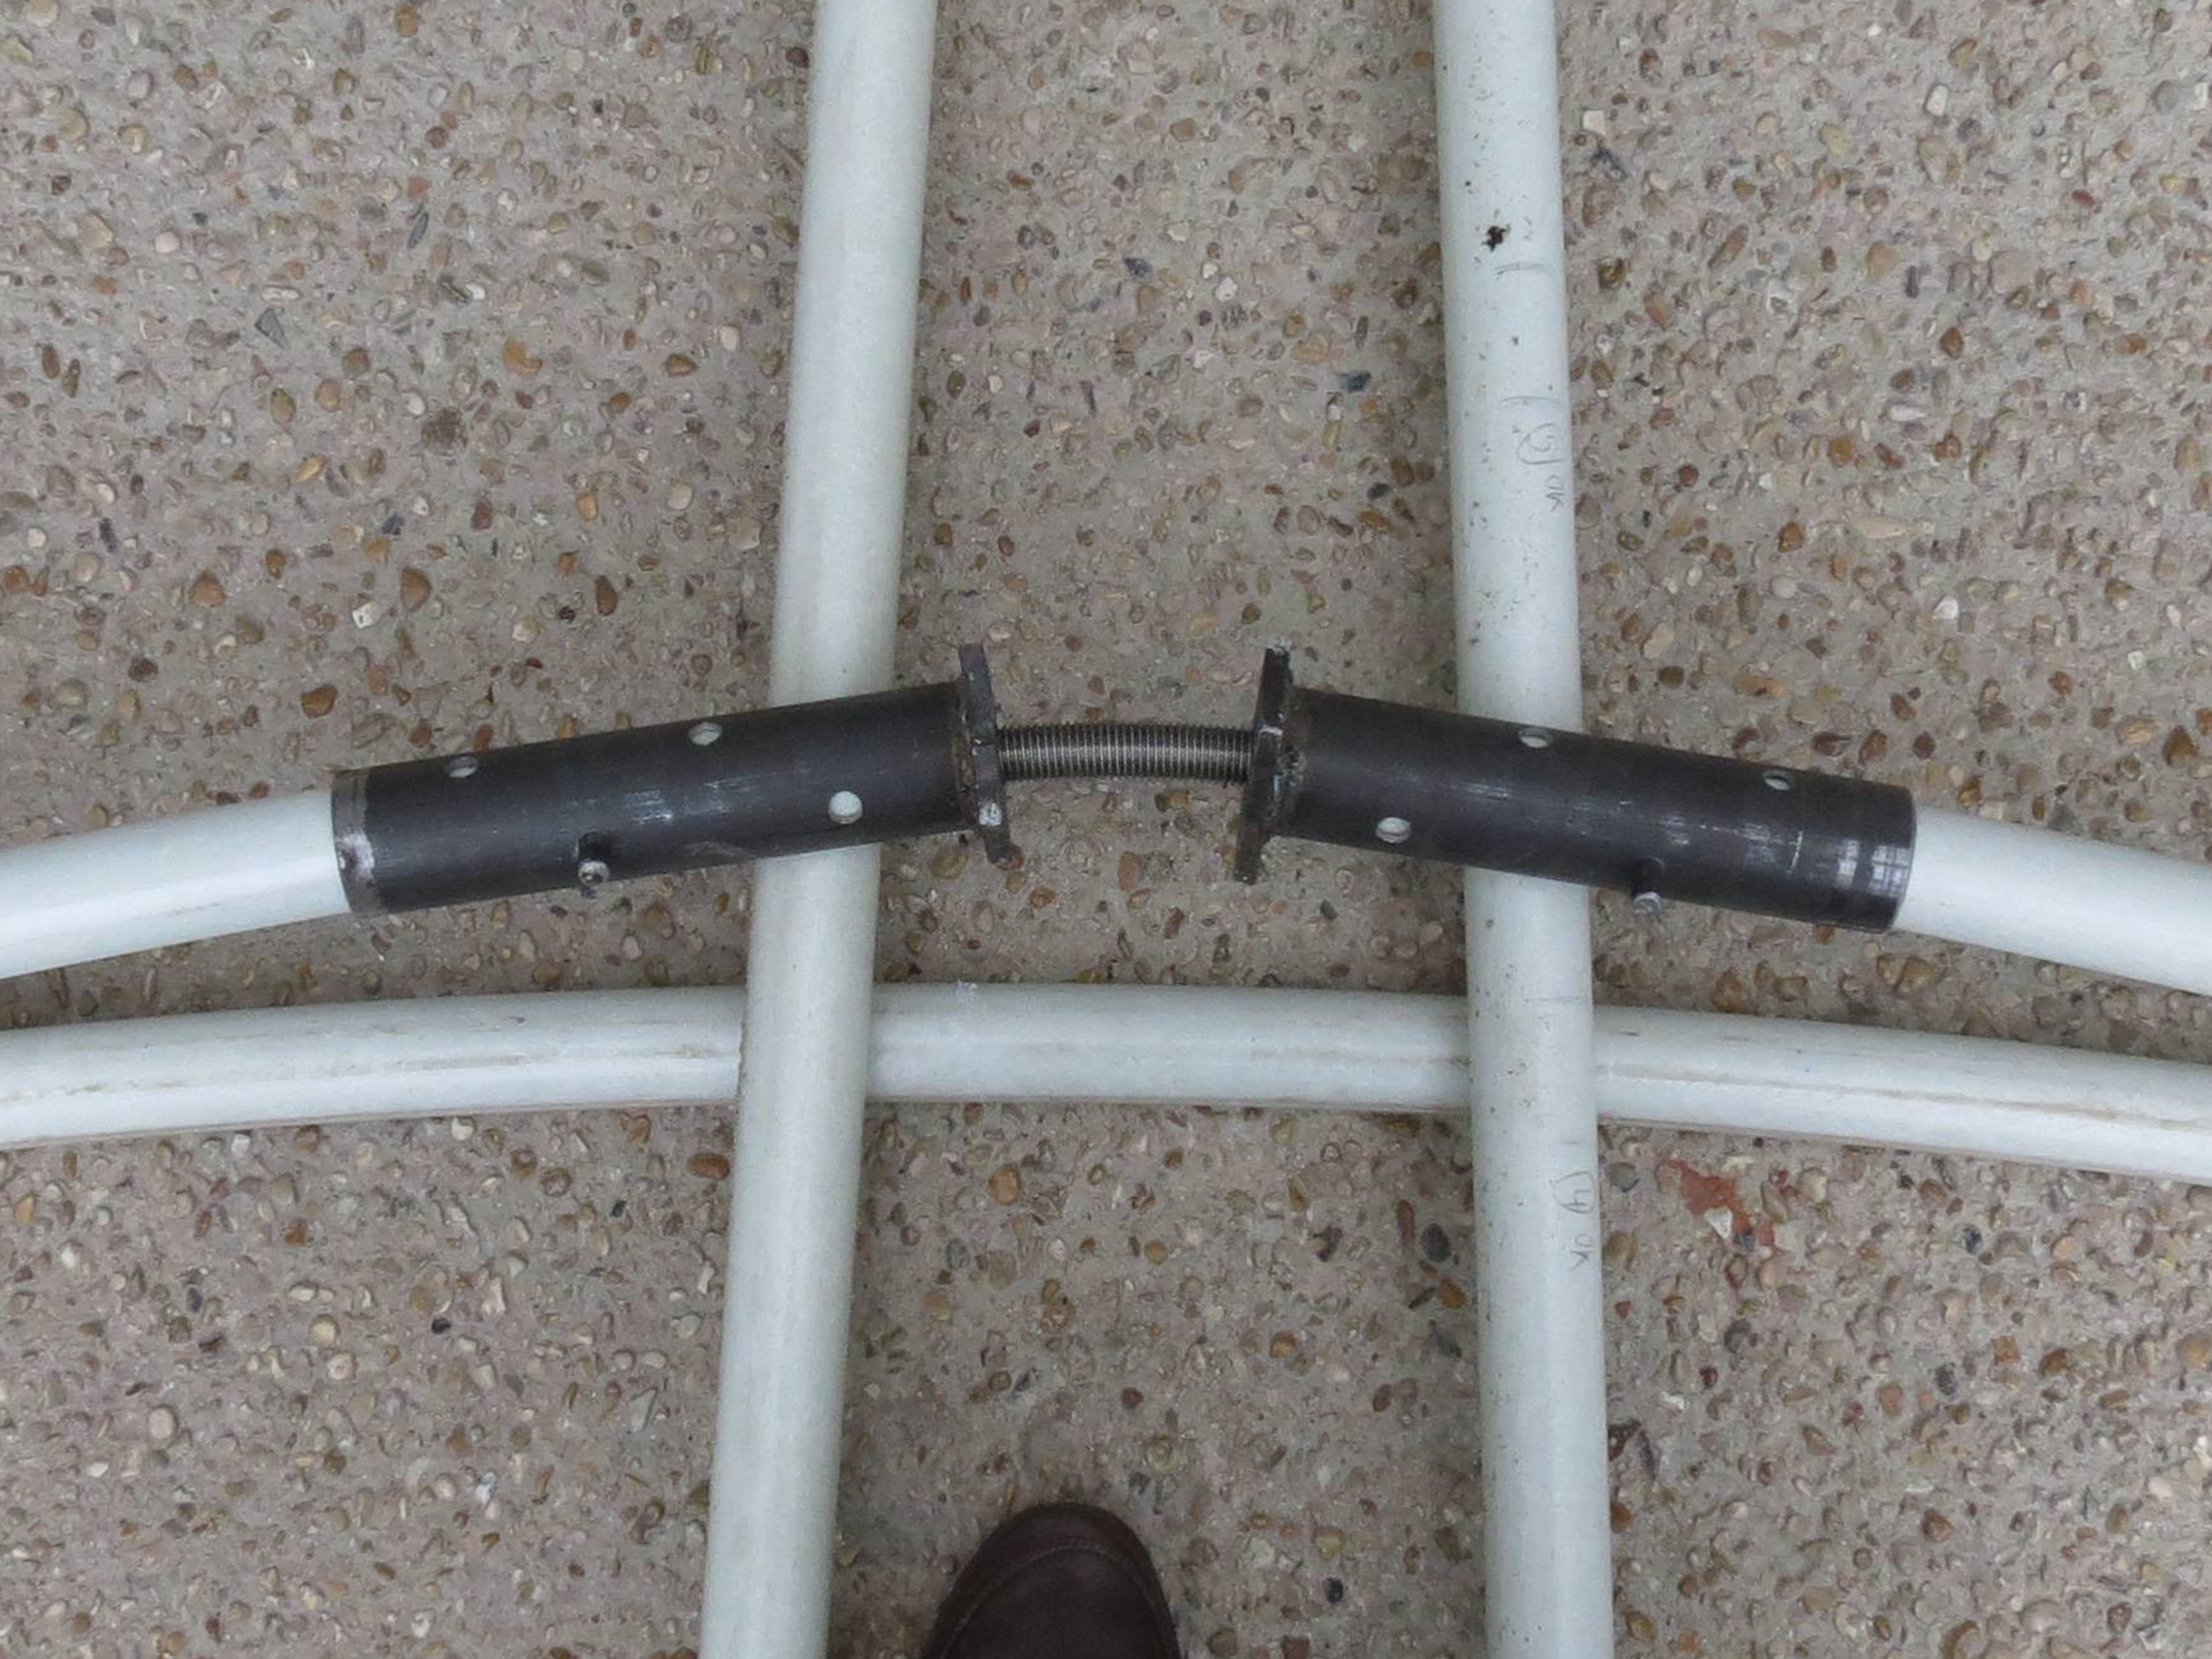
\includegraphics[width=0.48\textwidth]{sleeve4.jpg}\label{fig:sleeve_d}}\\
% 	\caption[Design and behavior of the the sleeve system]{Design and behavior of the the sleeve system.}
% 	\label{fig:sleeve_bench}
% 	%
% 	\vspace{0.75cm}
% 	%
% 	\subfloat[][Tearing]{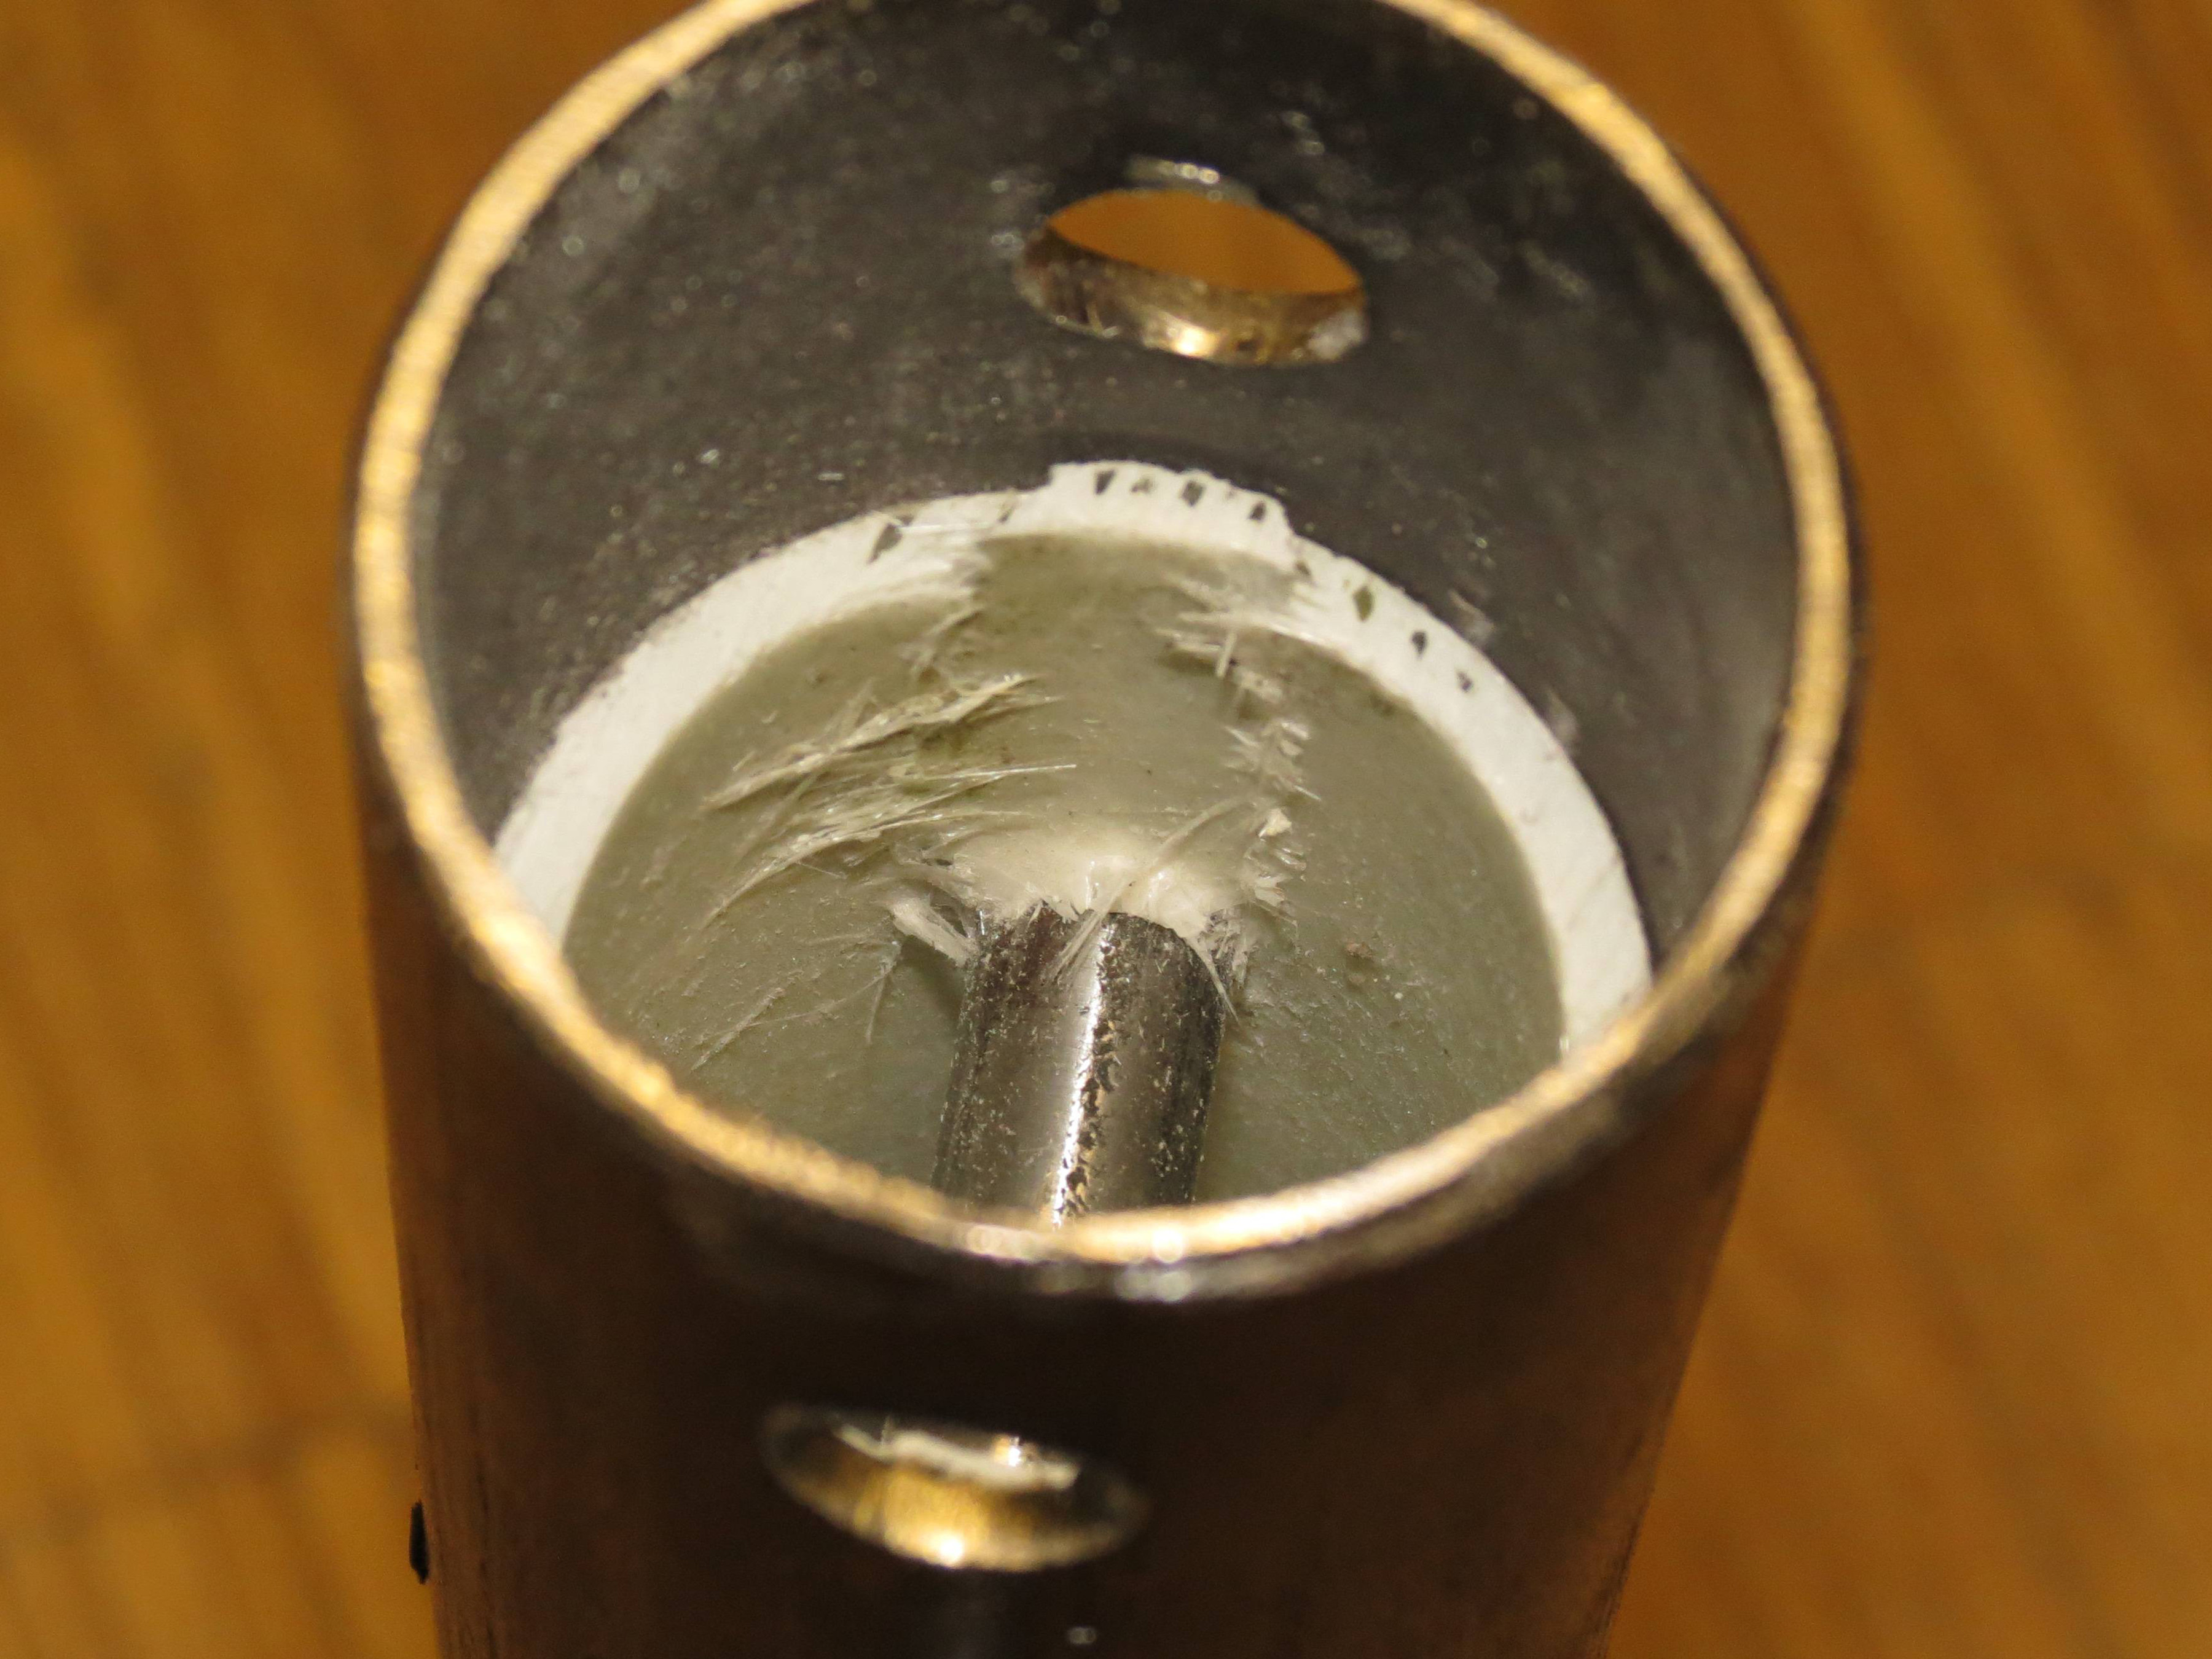
\includegraphics[width=0.48\textwidth]{pin.jpg}\label{fig:sleeve_e}}
% 	\hspace*{\fill}
% 	 \subfloat[][Contact compression]{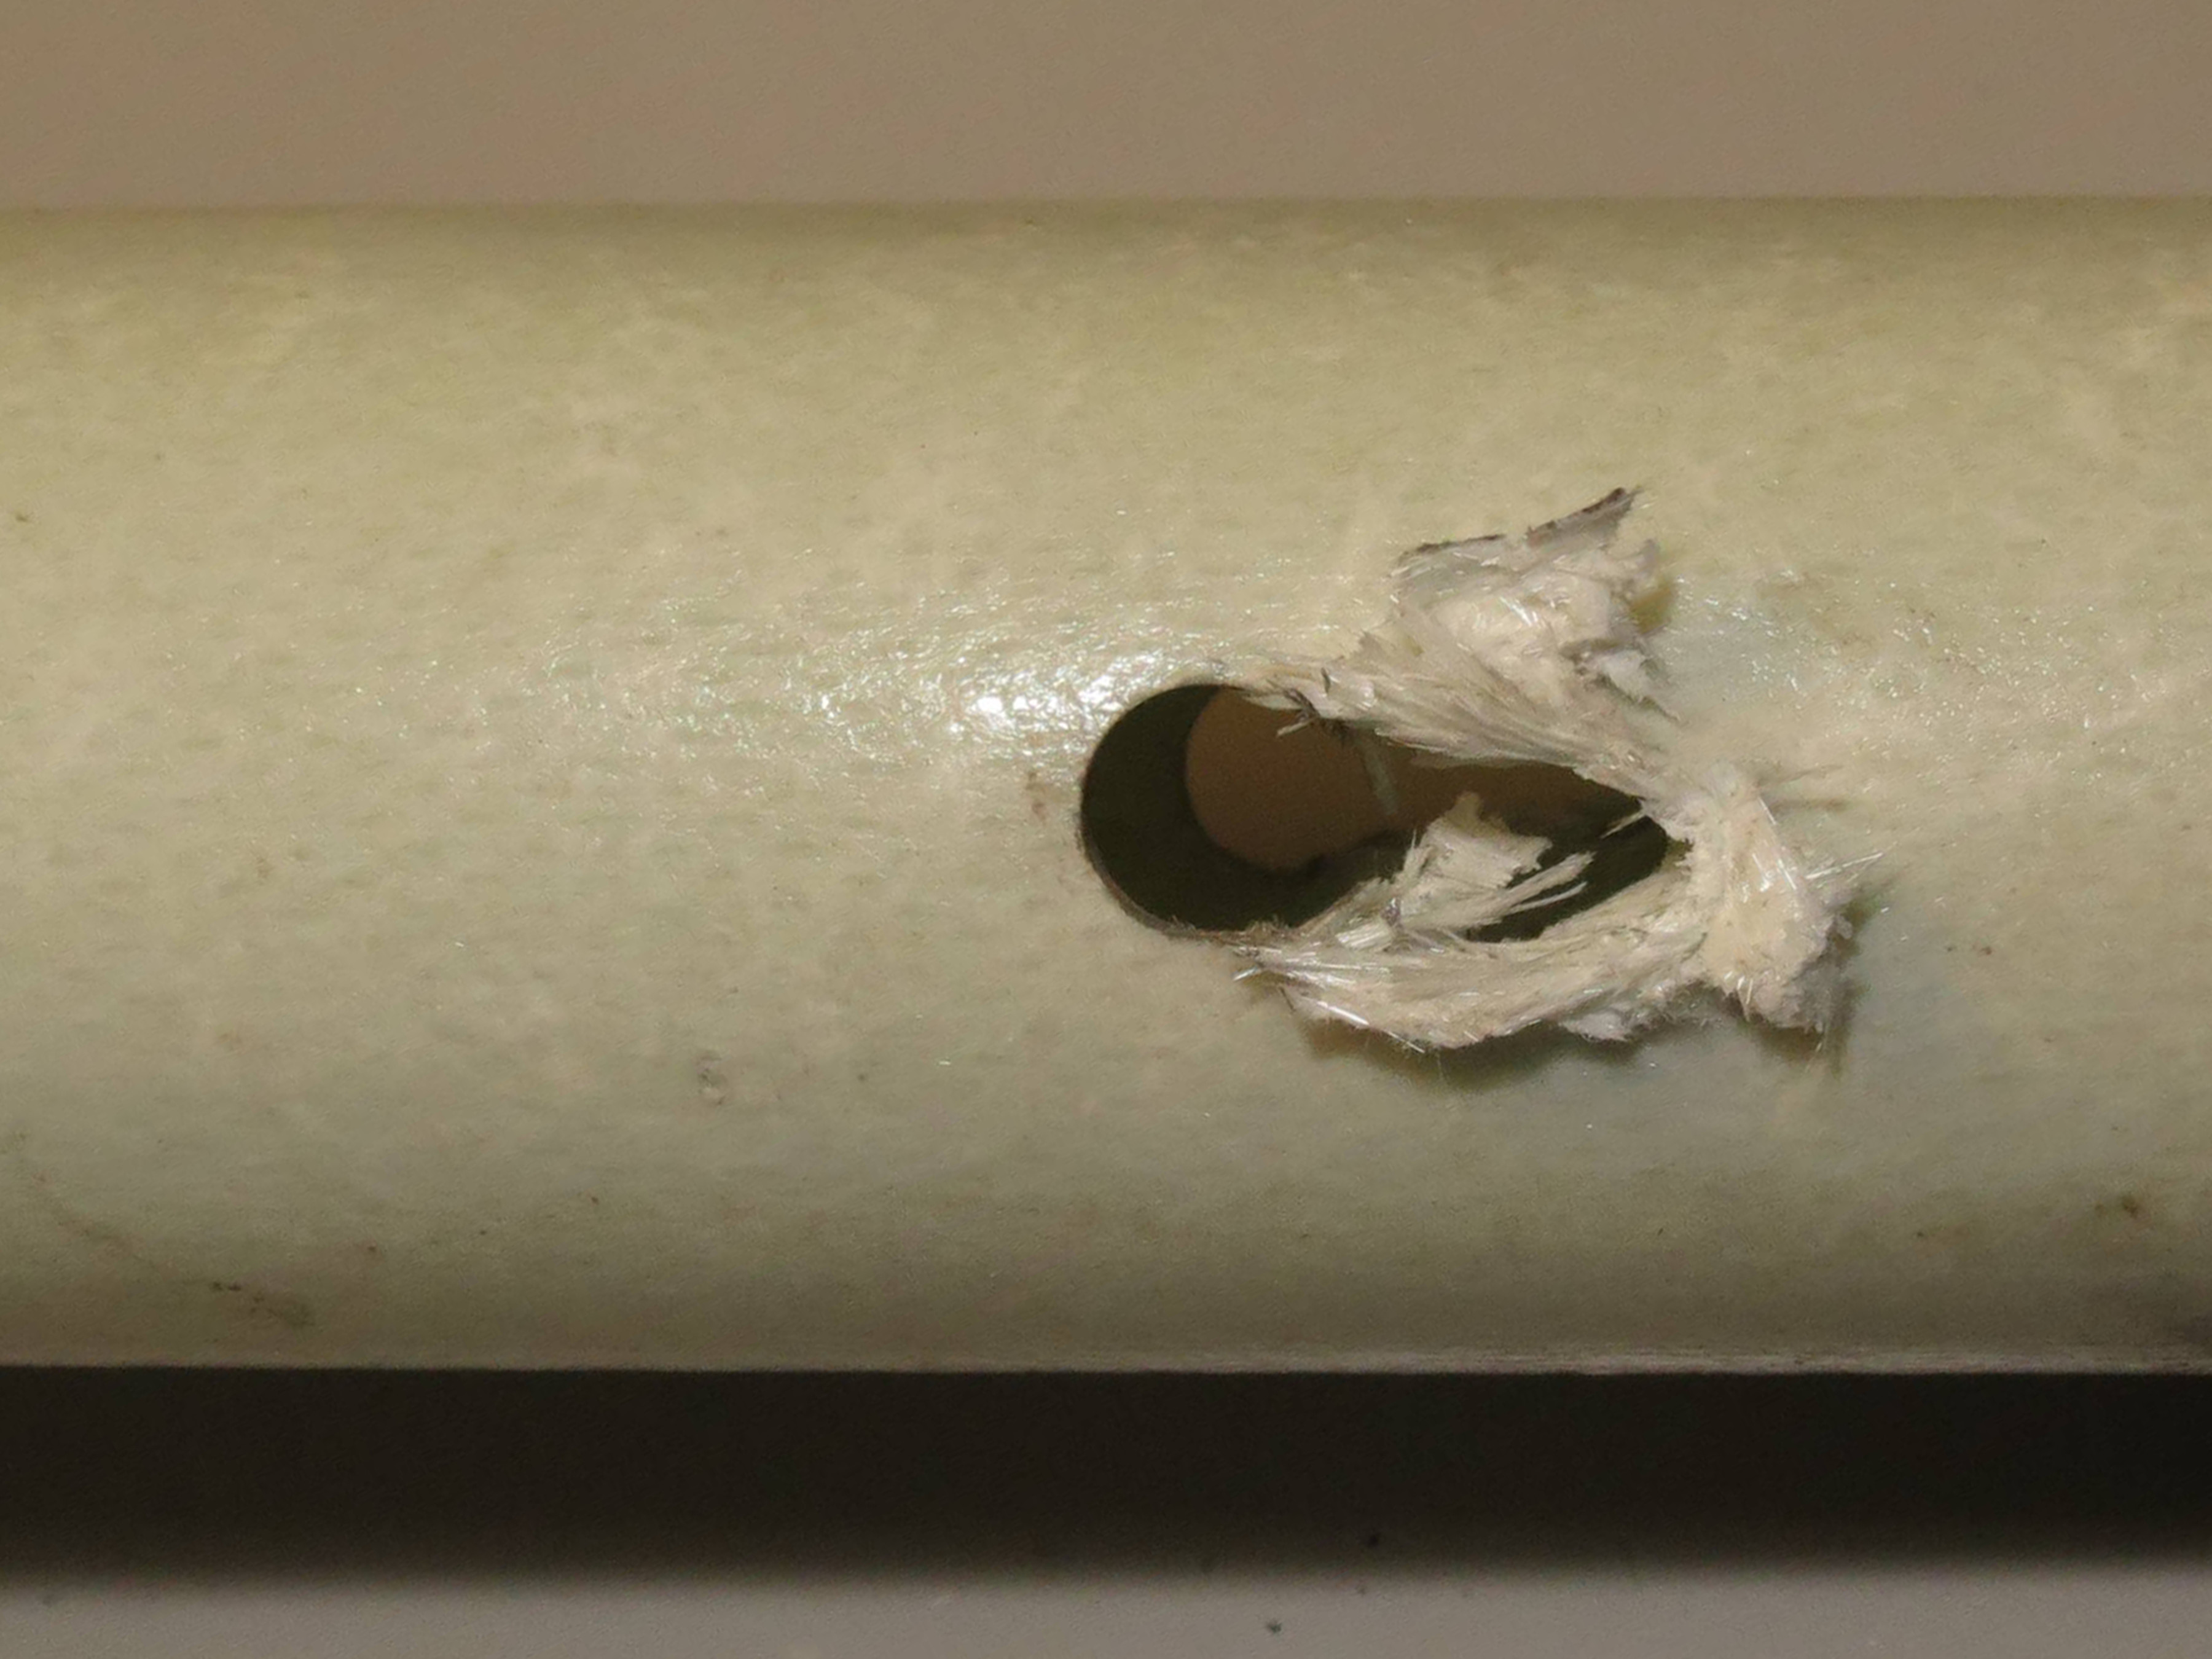
\includegraphics[width=0.48\textwidth]{pin2.jpg}\label{fig:sleeve_f}}\\
% 	\caption[Typical failure modes when testing the sleeve system in traction]{Typical failure modes when testing the sleeve system in traction.}
% 	\label{fig:sleeve_failure}
% 	\end{fullpage}
% \end{figure}

% \begin{figure}[p]
% \centering
% \begin{fullpage}
% 	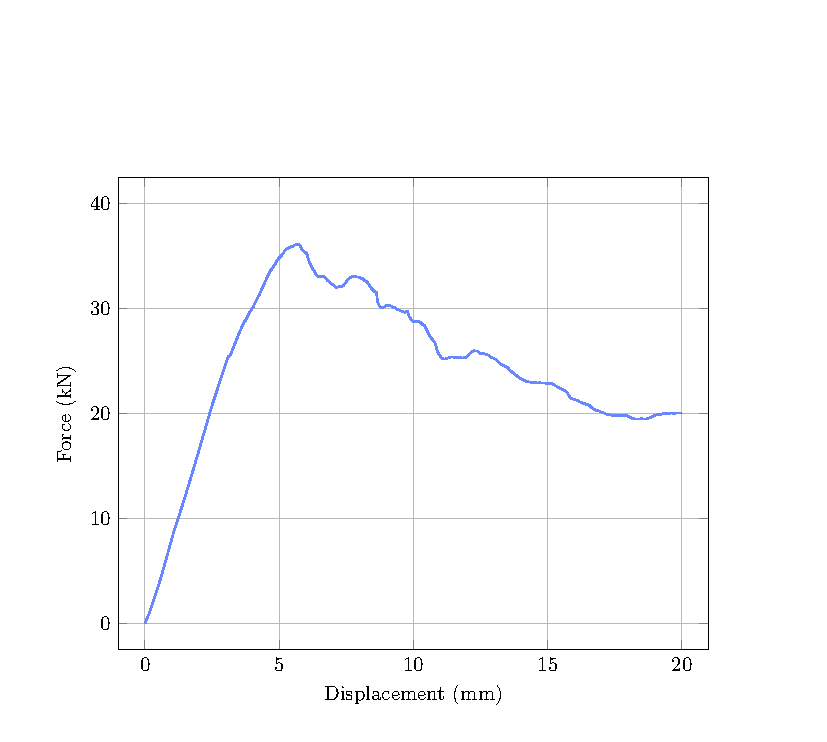
\includegraphics[]{ch3_creteil/plot/6_pin/build.pdf}
% 	\caption[Tensile test of the pinned connection]{Tensile test of the pinned connection. Results from \cite{Tayeb2015a}.}
% 	\label{plot:pintest}
% \end{fullpage}
% \end{figure}

% \begin{figure}[p]
% 	%
%      	\centering
% 	\begin{fullpage}
% 		\subfloat[][Geometry]{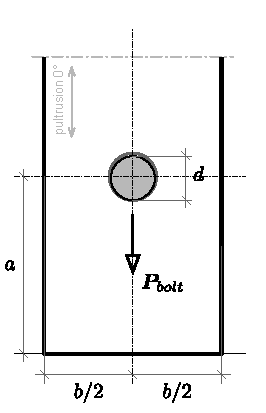
\includegraphics[]{breaking_1}\label{fig:breaking_1}}
% 		\subfloat[][Fibres]{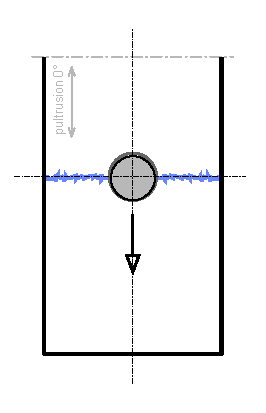
\includegraphics[]{breaking_2}\label{fig:breaking_2}}
% 		\subfloat[][Cleavage]{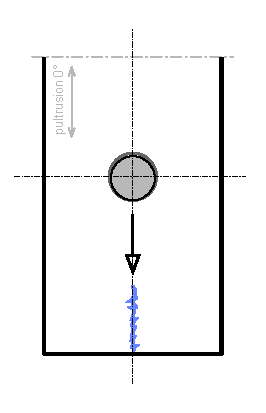
\includegraphics[]{breaking_3}\label{fig:breaking_3}} \\
% 		%
% 		\subfloat[][Tearing]{\includegraphics[]{breaking_4}\label{fig:breaking_4}}
% 		\subfloat[][Inclined compression]{\includegraphics[]{breaking_5}\label{fig:breaking_5}}
% 		\subfloat[][Contact compression]{\includegraphics[]{breaking_6}\label{fig:breaking_6}}
% 		%
% 		\vspace{10pt}
% 		\caption[Typical failure modes of a bolt in a pultruded element ]{Typical failure modes of a bolt in a pultruded element (\SI{0}{\degree}) \cite{Clarke2003}.}
% 		\label{fig:breaking}
% 	\end{fullpage}
% \end{figure}

\pagebreak
\subsection{Foundations}
%------------------------------------------
The detail of the footing was of major interest because it concentrated lots of technical difficulties and also had a strong visual impact (see \cref{fig:anchorage_dwg}).

The gridshell is fixed to the concrete strip thanks to the steel anchorages (6-15). Only the first two layers of tubes are fixed to the ground or doors (4, 3). The anchorage is made of two parts~: a steel connector (7) is pinned (6) to the composite tube (4) and equipped with a rotating steel clevis (9) ; a steel plate (15) is pinned to the concrete strip footing (26) and mounted with a vertical rotating steel clevis (11). The gridshell is connected to the ground by pinning the two parts of the anchorage. The three axis of rotations of the anchorage system -- one for each clevis axis and one for the axis of the common pin -- allow to accommodate any orientations of the tube. Moreover, the rotation of the clevis is ensured by simple bolts (9,12) and nuts (8,13) that allow some adjustments in length. The system provides a quick and easy fixing of the gridshell capable of all the necessary adjustments required in real mounting conditions.

The membrane (1) is laced (17) to a composite rod (19). This rod is bent and clamped every \SI{800}{mm} in a fixed scaffold collar (20) anchored in the concrete strip footing thanks to a steel part (21). This is a clever way to get a nice curved lacing rod at the bottom of the structure. The membrane strip (18) that ensures waterproofness is deported backward so that the lacing remains visible. This has a strong and elegant visible impact. This detail runs all around the structure and is reproduced around the doors. This member is subject to heavy shear forces from the tension of the lacing (around \SI{150}{daN/lm}) and this is why we chose a rod instead of a tube with a hollow section.

Thanks to the membrane strip and to a small step in the concrete slab (22) the water is evacuated into the drain, a simple trench full of gravels with two perforated flexible plastic pipes at the bottom.


\doubleblankpage[r]{%
	\hbox{}\thispagestyle{empty}
	\AddToShipoutPictureBG*{% 
		\Photo[
			node=PPbl,
			anchor=south west,
			gopt={width=\PaperWidth},
			]{anchorage2.pdf}%
		\savenodes{A}
		\PhotoCaptionRef[
			node=Atl, 
			anchor=north west,
			yshift=-\PhotoRefSkip, 
			phantom=true,
			]{figure}{}{Technical drawing of the footing}{fig:anchorage_dwg}
		\PhotoTextBox[
			node=CAtl,
			anchor=north west,
			border=false,
			]{%
				\figurecaption{fig:anchorage_dwg}
			}
	}
}{
	\hbox{}\thispagestyle{empty}
	\AddToShipoutPictureBG*{
		\SBox[%
			node=CAc,
			anchor=center,
			]{%
				\begin{tabular}{@{}l l r @{}}
					\toprule
					Item 								& Standard 			& Précontraint 702 Opaque Alu  \\
					\midrule
					Yarn 								& 					& 1100 dtex PES HT \\
					Weight 								& EN ISO 2286-2		& \SI{830}{g/m^2} \\
					Width 								& 					& \SI{267}{cm} \\
					Standard jumbo roll					& 					& \SI{50}{lm} or \SI{300}{lm}  \\
					Finish								& 					& 2-face acrylic varnish \\
					\midrule
					Tensile strength (warp/weft)		& EN ISO  1421		& \SI{280/280}{daN/ \SI{5}{\cm}} \\
					Tear strength (warp/weft)			& DIN 53.363		& \SI{30/28}{daN} \\
					Elongation under load (warp/weft)	& NF EN 15619		& < \SI{1}{\percent} / < \SI{1}{\percent} \\
					Adhesion							& EN ISO  2411		& \SI{10}{daN/ \SI{5}{\cm}} \\
					Solar transmission					& NFP 38511			& \SI{13.5}{\percent}  \\
					\midrule
					Flame retardancy					& NFP 92-507 		& M2 \\
														& DIN 4102-1 		& B1 \\
					Euroclass							& EN 13501-1 		& B-s2, d0 \\
					\midrule
					Cold resistance						& IS0 4675 			& \SI{-30}{\celsius} \\
					Heat resistance						& DIN 4102-1 		& \SI{+70}{\celsius} \\
					\bottomrule
				\end{tabular}
			}
		\PhotoCaptionRef[
			node=CAtl, 
			anchor=north west, 
			phantom=true,
			]{table}{}{Technical properties of the membrane}{tab:membrane}
		\PhotoTextBox[
			node=CAbl,
			anchor=south west,
			width=0.6\textwidth,
			border=false,
			]{\tablecaption{tab:membrane}}
	}
}


\subsection{The membrane}
%------------------------------------------
The membrane is nothing but a tailor-made one-piece clothing manufactured to dress up the structure. It was prefabricated based on the 3D model of the shape computed during the form-finding process (see \cref{sec=form-finding}) and not on some on-site geometric survey like for the prototypes presented in \cref{fig:proto}. The technical properties of the PVC coated fabric can be found in \cref{tab:membrane}.

\section{Hygrothermal behavior}\label{sec=hygro}
%------------------------------------------
\subsection{Temperature}\label{sec=temperature}
During the first two years and a half of its service life, the building has shown that the thermal comfort was far from ideal as the membrane has very poor thermal properties (see \cref{tab:membrane})~:
\begin{itemize}
\item During winter, the confort is ensured during Mass by a forced-air heating system positioned on the equipments slab, few meters away from the main structure. This solution is adapted to infrequent occupations of the building. In that case, the energetic cost remains limited even if the solution is far from optimal because of the lack of insulation.
\item During summer, the temperature raises very fast when the sun shines. The forced-air system is used to ventilate the interior volume. But the comfort level is rapidly insufficient as the interior temperature quickly exceeds \SI{30}{\celsius}. The discomfort is amplified as the membrane gets very hot and radiates toward the inside, increasing the feeling of warm. Consequently, there was no choice but to scheduled Mass earlier at this period of the year. Cooling was not possible for economic reasons as the building was used only few hours a week.
\end{itemize}


\doubleblankpage[l]{%
	\setlength{\tmpwidth}{0.8\textwidth}
	\hbox{}\thispagestyle{empty}
	\AddToShipoutPictureBG*{%
	\Photo[
		node=CAt,
		anchor=north,
		yshift=-\PhotoSkip,
		gopt={width=\tmpwidth},
		]{ch3_creteil/plot/5_thermal/build_Text.pdf}
	\savenodes{A}
	\Photo[
		node=Ab,
		anchor=north,
		yshift=\PhotoSkip,
		gopt={width=\tmpwidth},
		]{ch3_creteil/plot/5_thermal/build_Rad.pdf}
	\savenodes{B}
	%%
	\PhotoCaptionRef[
		node=Atl, 
		anchor=north west, 
		phantom=true,
		]{figure}{Weather data at site location during opening hours}{Weather data at site location during opening hours (8:00 AM to 7:00 PM)}{fig:thermal_ext}
	\PhotoCaptionRef[
		hrefnode=Atl, 
		node=Atr, 
		anchor=north east,
		xshift=-0.75cm,
		yshift=-0.85cm,
		]{subfigure}{}{Temperature}{plot:T_1}
	\PhotoCaptionRef[
		hrefnode=Btl, 
		node=Btr, 
		anchor=north east,
		xshift=-0.75cm,
		yshift=-0.85cm,
		]{subfigure}{}{Solar radiation}{plot:T_2}
	\PhotoTextBox[
		node=CAbl,
		anchor=south west,
		width=\textwidth,
		border=false,
		]{%
			\figurecaption{fig:thermal_ext}\par
			\figurecaption{plot:T_1}\par
			\figurecaption{plot:T_2}
		}
	}
}{%
	\hbox{}\thispagestyle{empty}
	\AddToShipoutPictureBG*{%
	\Photo[
		node=CAt,
		anchor=north,
		yshift=-\PhotoSkip,
		gopt={width=\tmpwidth},
		]{ch3_creteil/plot/5_thermal/build_Tint_noV.pdf}
	\savenodes{A}
	\Photo[
		node=Ab,
		anchor=north,
		yshift=\PhotoSkip,
		gopt={width=\tmpwidth},
		]{ch3_creteil/plot/5_thermal/build_Tint_V.pdf}
	\savenodes{B}
	%%
	\PhotoCaptionRef[
		node=Atl, 
		anchor=north west, 
		phantom=true,
		]{figure}{Temperature inside the building during opening hours}{Temperature inside the building during opening hours (8:00 AM to 7:00 PM)}{fig:thermal_int}
	\PhotoCaptionRef[
		hrefnode=Atl, 
		node=Atr, 
		anchor=north east,
		xshift=-0.75cm,
		yshift=-0.85cm,
		]{subfigure}{}{Without ventilation}{plot:T_3}
	\PhotoCaptionRef[
		hrefnode=Btl, 
		node=Btr, 
		anchor=north east,
		xshift=-0.75cm,
		yshift=-0.85cm,
		]{subfigure}{}{With ventilation}{plot:T_4}
	\PhotoTextBox[
		node=CAbl,
		anchor=south west,
		border=false,
		width=\textwidth,
		]{%
			\figurecaption{fig:thermal_int}\par
			\figurecaption{plot:T_3}\par
			\figurecaption{plot:T_4}
		}
	}
}

At the time of writing, the building is being reconfigured and so its purpose is changing. A better thermal comfort is now required and solutions have to be found. Thus, a study on the thermal behavior of the structure has been done.\footnote{This study was done in June 2017 by the design companies T/E/S/S and CHOULET for the reconfiguration project of the temporary cathedral.} The main results are gathered in this thesis. The monthly exterior temperatures observed at the site location from 8:00 AM to 7:00 PM, which corresponds to the new intended opening hours of the building, are presented in \cref{plot:T_1}. Note that the maximum value is given over one hour, that is the observed temperature exceeds this value during a one-hour-wide window in the day. The solar radiation is also given in \cref{plot:T_2}. Two scenarios are studied~:
\begin{enumerate}
\item The structure is completely closed. No ventilation is put in place. The interior temperature can reach \SI{70}{\celsius} (see \cref{plot:T_3}).
\item The structure is ventilated but no cooling system is put in place. The maximum interior temperature is lowered significantly but it can still reach \SI{50}{\celsius} (see \cref{plot:T_4}).
\end{enumerate}

This study confirms what the experience has shown : the temperature inside the building can be very high. Above \SI{30}{\celsius} this is problematic for the comfort of the people. Above \SI{50}{\celsius} and up to \SI{70}{\celsius} it becomes problematic for the building itself. Indeed, this level of temperature is closed to the heat resistance of the membrane (see \cref{tab:membrane}) ; the interface layer faces a serious decrease of its capacity to resist to sliding (\cref{plot:epdm_temperature}) ; the creep of GFRP tubes is speed up (\cref{sec=gfrp}).

\subsection{Moisture}
Condensation was also noticed in winter and shoulder season. Sometimes, droplets of water could fall abundantly and thus the wooden furnitures had to be protected. This phenomenon was particularly intense the first months because the concrete slab had not yet fully dry-out. To protect the structure and the furnitures, it was decided to maintain the inside temperature above \SI{10}{\celsius} at all times.


% \begin{figure}[p]
% 	%
%      	\centering
% 	\begin{leftfullpage}
% 		\subfloat[][Temperature.]{\includegraphics[]{ch3_creteil/plot/5_thermal/build_Text.pdf}\label{plot:T_1}} \\
% 		\subfloat[][Solar radiation.]{\includegraphics[]{ch3_creteil/plot/5_thermal/build_Rad.pdf}\label{plot:T_2}} \\
% 		\vspace{10pt}
% 		\caption[Weather data at site location during opening hours]{Weather data at site location during opening hours (8:00 AM to 7:00 PM).}
% 		\label{fig:thermal_ext}
% 	\end{leftfullpage}
% \end{figure}
% \begin{figure}[p]
% 	%
%      	\centering
% 	\begin{fullpage}
% 		\subfloat[][Without ventilation.]{\includegraphics[]{ch3_creteil/plot/5_thermal/build_Tint_noV.pdf}\label{plot:T_3}} \\
% 		\subfloat[][With ventilation.]{\includegraphics[]{ch3_creteil/plot/5_thermal/build_Tint_V.pdf}\label{plot:T_4}} \\
% 		\vspace{10pt}
% 		\caption[Temperature inside the building during opening hours]{Temperature inside the building during opening hours (8:00 AM to 7:00 PM).}
% 		\label{fig:thermal_int}
% 	\end{fullpage}
% \end{figure}


% \clearpage
\section{Cost analysis}\label{sec=costanalysis}
%------------------------------------------
\subsection{Overall cost for the client}
The overall cost of the project -- that is the amount of money paid by the client -- was estimated to 324\,000~€ excluding taxes (see \cref{fig:budget}). This price includes all the possible costs related to the construction of the project~: the cost of the main building (masonry, doors, gridshell, envelop, fittings, heating, electricity, lightning, drainage, sewage, etc.), the cost of the service building, the cost of pedestrian pathways, the cost of the design studies, etc.

However, this cost does not take into account all the (free) man-hours spent by the volunteers to prefabricate, assemble, erect and brace the gridshell. The real cost of the gridshell system, when a cost is put on this labor, is estimated in \cref{sec=gs_cost}.


\doubleblankpage[r]{%
	\hbox{}\thispagestyle{empty}
	\AddToShipoutPictureBG*{%
	\Photo[
		node=CAc,
		anchor=center,
		gopt={width=\textwidth},
		]{budget}
	\savenodes{A}
	%%
	\PhotoCaptionRef[
		node=Atl, 
		anchor=north west, 
		phantom=true,
		]{figure}{}{Cost allocation for the whole project}{fig:budget}
	\PhotoTextBox[
		node=CAbl,
		anchor=south west,
		width=\textwidth/2,
		border=false,
		]{%
			\figurecaption{fig:budget}
			This is the estimated overall final cost charged to the client. Prices are given excluding taxes (V.A.T).
		}
	}
}{%
	\hbox{}\thispagestyle{empty}
	\AddToShipoutPictureBG*{%
	\Photo[
		node=CAc,
		anchor=center,
		gopt={width=\textwidth},
		]{building}
	\savenodes{A}
	%%
	\PhotoCaptionRef[
		node=Atl, 
		anchor=north west, 
		phantom=true,
		]{figure}{}{Cost allocation per square meter of covered area}{fig:building}
	\PhotoTextBox[
		node=CAbl,
		anchor=south west,
		width=\textwidth/2,
		border=false,
		]{%
			\figurecaption{fig:building}\par\medskip
			The cost of design is not included as it would not be representative. Prices are given excluding taxes (V.A.T).
		}
	}
}

Moreover, this project required a lot of design studies and tests to verify the material properties and to validate the strength of key elements such as the swivel coupler with its EPDM layer, the sleeve system and the ground anchorage. The real cost of the studies was by far higher than what was really charged to the client and the difference must be regarded as an investment from the company T/E/S/S. In the same manner, people from the laboratory gave a consistent support during the construction stage as they were the only available experienced workers familiar with the construction of elastic gridshells in composite material \cite{Douthe2010a,Baverel2012} and this labor was not charged back to the client.

The project was favorably accepted by the client based on the estimation that the cost of the gridshell would not be more expensive by 30\% than renting a simple tent. The rental of a 400~m\textsuperscript{2} tent with its floor was evaluated to 110\,000~€ for a period of time of 18 months. Retrospectively this target was met, especially as the cathedral was finally used for almost two years and a half, far more than the 18 months expected initially, and with no additional cost because the diocese owned the building.

% \begin{figure}[h]
% \begin{fullpage}
% \centering
% 	\includegraphics[]{budget}\vspace{10pt}
% 	\caption[Cost allocation for the whole project]{Cost allocation for the whole project. This is the estimated overall final cost charged to the client. Prices are given excluding taxes (V.A.T).}
% 	\label{fig:budget}
% 	%
% 	\vspace{2cm}
% 	%
% 	\includegraphics[]{building}\vspace{10pt}
% 	\caption[Cost allocation per square meter of covered area]{Cost allocation per square meter of covered area. The cost of design is not included as it would not be representative. Prices are given excluding taxes (V.A.T).}
% 	\label{fig:building}
% 	\end{fullpage}
% \end{figure}

\subsection{Cost details for the building}\label{sec=gs_cost}
Here we present the cost details for the main building, that is the cathedral itself. We try to understand what is the true cost of the gridshell system in this particular project and we thus eliminate side costs (for instance the cost of fittings, the cost of the pedestrian pathways, the cost of the service building, etc.). The cost allocation is presented per square meter of covered area in \cref{fig:building}. The total price for the building, excluding studies, is 473~€/m\textsuperscript{2}. It is composed of :
\begin{itemize}
\item  100~€/m\textsuperscript{2}~: the cost of masonry works (levelling, footings, slab, drainage) detailed in \cref{tab:masonry}. This construction works were made by a professional contractor named BATEM.
\item  248~€/m\textsuperscript{2}~: the cost of the superstructure (anchorages, gridshell, membrane covering and doors) detailed in \cref{tab:superstructure}. This price includes the labor of the volunteers (35~€/hour) and all the costs associated to construction of the structure, including the renting of all the necessary equipments (cranes, arial buckets, etc.).
\item  126~€/m\textsuperscript{2}~: the cost of the envelope (lacing rod, fabric, installation) detailed in \cref{tab:superstructure}. This construction works were made by a professional contractor named ESMERY CARON.
\end{itemize}

Here, the global amount of studies was charged around 83\,300~€, that is 248~€/m\textsuperscript{2} (see \cref{fig:budget}). This heavy cost was compensated by the fact that volunteers provided a lot of free labor (see \cref{fig:manhours}). In a more standard commercial context, the design process would be optimized too and the price of studies would go down to 15\% to 20\% of the price of the building, that is 70 to 95~€/m\textsuperscript{2}. This would bring the final price of the building to 550~€/m\textsuperscript{2}. This price is clearly high if only its sheltering capability is required regarding other technologies. However, if more than sheltering is mandatory, the quality and singularity of the space created here is probably worth the price ; then this technology becomes a lot more affordable than existing traditional systems that can materialized free-forms.


\doubleblankpage[l]{%
	\hbox{}\thispagestyle{empty}
	\AddToShipoutPictureBG*{%
		\SBox[%
			node=CAt,
			anchor=north,
			]{%
				\begin{tabularx}{\textwidth}{@{}Xrrrr@{}}
					\toprule
															& \multicolumn{2}{c}{Unit Task} 		& \multicolumn{2}{c}{Man-Hours}	 	\\
					\cmidrule(l){2-3} \cmidrule(l){4-5}
				 	Item 										& Worker 		& Duration		& Quantity 		& Hours			\\
					\midrule
					%
					\addlinespace[10pt]
					\textbf{Workstation \textquote{Cutting}}			& \tablebf{4}	& 				&				& \tablebf{20.53}	\\
					Pick a raw tube from the stock					& 2 			& 1'\,00''			& 176			& 5.87 			\\
					Mark it and cut it at right length					& 2 			& 2'\,00''			& 176			& 11.73			\\
					Put it into the labelling stock					& 2  			& 0'\,30''			& 176			& 2.93 			\\
					%
					\addlinespace[10pt]
					\textbf{Workstation \textquote{Labelling}}			& \tablebf{5}	&				&				& \tablebf{56.64} 	\\
					Pick a tube from the labelling stock				& 2 			& 1'\,00''			& 176			& 5.87 			\\
					Label it at start and end						& 2  			& 1'\,00''			& 176			& 5.87 			\\
					Mark the position of connection collars			& 1  			& 0'\,30''			& 2260			& 18.83			\\
					Mark the position of sleeves					& 1  			& 0'\,30''			& 250			& 2.08			\\
					Mark the position of anchorages				& 1  			& 0'\,30''			& 127			& 21.06			\\
					Put it into the prefabrication stock					& 2  			& 0'\,30''			& 176			& 2.93 			\\
					%
					\addlinespace[10pt]
					\textbf{Workstation \textquote{Prefabrication}}		&  \tablebf{6}   	&				& 				& \tablebf{67.75} 	\\
					Pick a tube from the prefabrication stock			& 2 			& 1'\,00''			& 176			& 5.87 			\\
					Put the EPDM ribbon						& 1 			& 0'\,30''			& 2260			& 18.83 			\\
					Prefix the swivel collar on the tube				& 1 			& 0'\,30''			& 565			& 4.71 			\\
					Glue	the sleeves							& 3  			& 2'\,00''			& 250			& 25.00			\\
					Drill pin holes for the sleeves					& 1  			& 1'\,00''			& 250			& 4.16			\\
					Fix sleeve pins 								& 1  			& 1'\,30''			& 250			& 6.25			\\
					Put it into the final stock						& 2  			& 0'\,30''			& 176			& 2.93 			\\
					%
					\addlinespace[10pt]
					\textbf{Workstation \textquote{Site Assembly}}		&  \tablebf{12}   &				& 				& \tablebf{107.34} 	\\
					Connect the sleeves with steel rods 				& 5 			& 5'\,00''			& 125			& 52.08 			\\
					Pick a tube and position it in the grid 				& 2 			& 3'\,00''			& 176			& 17.60 			\\
					Install swivel couplers (HV)					& 1 			& 2'\,00''			& 565			& 18.83 			\\
					Controlled tightening of couplers (HV)			& 1 			& 1'\,00''			& 1130			& 18.83 			\\
					%
					\addlinespace[10pt]
					{Workstation \textquote{Grid Erection}}			& {12}   		& 8:00'\,00''		& 1				& {96.00} 	\\
					{Workstation \textquote{Grid Bracing}}			& {6}   		& 8:00'\,00''		& 3				& {144.00} 	\\
					%
					\addlinespace[10pt]
					\midrule
					Grid prefabrication 							& 			& 				&				&{252.00}  		\\
					Grid erection 								& 			& 				&				&{96.00}  			\\
					Grid bracing 								& 			& 				&				&{144.00}  		\\
					Cost of supervision (15\%)					& 			&				&				& {74.00}  			\\
					\textbf{Total} 								& 			& 				&				& \tablebf{566.00}  	\\
					\bottomrule
				\end{tabularx}
			}
		\PhotoCaptionRef[
			node=TL, 
			anchor=north west, 
			% yshift=-\PhotoRefSkip,
			phantom=true,
			]{table}{}{Man-hours spent by the volunteers on the fabrication}{tab:manhours}
		\PhotoTextBox[
			node=CAbl,
			anchor=south west,
			width=0.6\textwidth,
			border=false,
			]{%
				\tablecaption{tab:manhours}\par\medskip
				A 15\% increase is considered to take into account coordination and supervision of the individual tasks. See \cref{fig:manhours} for a graphical representation of these data.
			}
	}
}{%
	\hbox{}\thispagestyle{empty}
	\AddToShipoutPictureBG*{%
	\Photo[
		node=CAc,
		anchor=center,
		gopt={width=\textwidth},
		]{manhours}
	\savenodes{A}
	%%
	\PhotoCaptionRef[
		node=Atl, 
		anchor=north west, 
		phantom=true,
		]{figure}{}{Allocation of the man-hours spent by the volunteers}{fig:manhours}
	\PhotoTextBox[
		node=CAbl,
		anchor=south west,
		width=\textwidth/2,
		border=false,
		]{%
			\figurecaption{fig:manhours}\par\medskip
			A 15\% increase is considered to take into account coordination and supervision of the individual tasks. See \cref{tab:manhours} for detailed data.
		}
	}
}

\doubleblankpage[l]{%
	\hbox{}\thispagestyle{empty}
	\AddToShipoutPictureBG*{%
		\SBox[%
			node=CAt,
			anchor=north,
			]{%
				\begin{tabularx}{\textwidth}{@{}Xlrrr@{}}
					\toprule
				 	Item	 							& Unit				& Quantity		& U.P. (€)			& Price (€) 			\\
					\midrule
					\addlinespace[10pt]
					Building implantation 				& 					& 1			& 1\,300.00		& 1\,300.00  			\\
					%
					\addlinespace[10pt]
					\textbf{Leveling works } 				& 					& 			& 				& \tablebf{11\,680.00}  			\\
					Top soil stripping  					& m\textsuperscript{2}	& 400		& 10.00			&  4\,000.00  			\\
					Trench for concrete strip footing  		& ml					& 76			& 30.00			&  2\,280.00  			\\
					Earth removal  						& m\textsuperscript{3}	& 180		& 30.00			&  5\,400.00  			\\
					%
					\addlinespace[10pt]
					\textbf{Concrete} 					& 					& 			& 				& \tablebf{17\,400.00}  	\\
					Concrete strip footing (200~kg/m\textsuperscript{3} steel) & ml		& 70			& 30.00			&  2\,100.00  			\\
					Concrete slab (x2 welded wire mesh) 	& m\textsuperscript{2}	& 340		& 45.00			&  15\,300.00  			\\
					%
					\addlinespace[10pt]
					\textbf{Drainage systems} 				& 					& 			& 				& \tablebf{4\,500.00}  	\\
					French drain (x2 \O 100~mm pipes)		& ml					& 70			& 30.00			&  2\,100.00  			\\
					Precast concrete inspection chamber 	& 					& 1			& 400.00			&  400.00  			\\
					Drain line (PVC \O 125~mm pipe)		& ml					& 30			& 30.00			&  900.00  			\\
					Pre-assembled channel drain			& ml					& 10			& 110.00			&  1\,100.00  			\\
					%
					\addlinespace[10pt]
					\midrule
					\textbf{Masonry works} 				& €/m\textsuperscript{2}	& 350 		& \tablebf{100}		& \tablebf{34\,880.00}  	\\
					\bottomrule
				\end{tabularx}
			}
		\PhotoCaptionRef[
			node=TL, 
			anchor=north west, 
			% yshift=-\PhotoRefSkip,
			phantom=true,
			]{table}{}{Cost allocation for masonry works}{tab:masonry}
		\PhotoTextBox[
			node=CAbl,
			anchor=south west,
			width=0.6\textwidth,
			border=false,
			]{%
				\tablecaption{tab:masonry}\par\medskip
				Prices are given excluding taxes (V.A.T). Only costs associated to the structure are reported here ; for instance the works for the equipment slab and the pathways are omitted. See \cref{tab:masonry} for detailed data.
			}
	}
}{%
	\hbox{}\thispagestyle{empty}
	\AddToShipoutPictureBG*{%
	\Photo[
		node=CAc,
		anchor=center,
		gopt={width=\textwidth},
		]{masonry}
	\savenodes{A}
	%%
	\PhotoCaptionRef[
		node=Atl, 
		anchor=north west, 
		phantom=true,
		]{figure}{}{Cost allocation for masonry works}{fig:masonry}
	\PhotoTextBox[
		node=CAbl,
		anchor=south west,
		width=\textwidth/2,
		border=false,
		]{%
			\figurecaption{fig:masonry}\par\medskip
			Prices are given excluding taxes (V.A.T). Only costs associated to the structure are reported here ; for instance the works for the equipment slab and the pathways are omitted. See \cref{tab:masonry} for detailed data.
		}
	}
}

\doubleblankpage[l]{%
	\hbox{}\thispagestyle{empty}
	\AddToShipoutPictureBG*{%
		\SBox[%
			node=CAt,
			anchor=north,
			% yshift=1cm,
			]{%
				\begin{tabularx}{\textwidth}{@{}Xlrrr@{}}
					\toprule
				 	Item	 							& Unit				& Quantity		& U.P. (€)		& Price (€) 			\\
					\midrule
					\addlinespace[10pt]
					\textbf{Manufacturing of the gridshell} 	& 					& 			& 				& \tablebf{42\,853}  	\\
					GRFP tube (\O 42~mm)				& ml					& 2304		& 3.66			&  8\,433  			\\
					Swivel connector (42x42~mm)			& 					& 1295		& 3.95			&  5\,115  			\\
					Swivel connector (42x49~mm)			& 					& 135		& 4.18			&  564  			\\
					EPDM layer (1302x40x1.5~mm ribbon)	& 					& 2775		& 0.36			&  1131  			\\
					Welded steel sleeve system			& 					& 150		& 50.00			&  7\,500  			\\
					ARALDIT 2047 glue (480~ml cartridge)	& 					& 8			& 45.00			&  360 			\\
					Ground anchorage (welded steel)		& 					& 120		& 80.00			&  9\,600  			\\
					Man-hours (prefabrication)			& h 					& 290		& 35.00			& 10\,150			\\
					%
					\addlinespace[10pt]
					\textbf{Manufacturing of the envelope}	& 					& 			& 				& \tablebf{34\,769}  	\\
					GFRP lacing rod (\O 32~mm) 			& ml 					& 96			& 14.00			&  1\,134  			\\
					Steel clip for the rod					&  					& 125		& 15.00			&  1\,875  			\\
					Swivel collar (\O 34~mm)				& 					& 120		& 3.50			&  420  			\\
					PVC coated fabric					& m\textsuperscript{2}	& 550		& 50.00			&  27\,500  		\\
					Option for transparent inclusion			& 					& 12			& 320.00			&  3\,840  			\\
					%
					\addlinespace[10pt]
					\textbf{Manufacturing of the steel doors} 					& 					& 			& 				& \tablebf{15\,000}  	\\
					Main door 						& 					& 1			& 10\,000.00		&  10\,000  		\\
					Small door  						&					& 1			& 5\,000.00		&  5\,000 			\\
					%
					\addlinespace[10pt]
					\textbf{On-site works of installation} 		& 					& 			& 				& \tablebf{38\,220}  	\\
					Installation of the doors				& 					& 1			& 5\,000.00		&  5\,000  			\\
					Installation of the anchorages and clips	& h					& 90			& 45.00			&  4\,050  			\\
					Grid erection 						& h					& 110		& 35.00			&  3\,850  			\\
					\quad {cranes (x2 35T)}				& h					& 24			& 110.00			&  2\,640  			\\
					Grid bracing 						& h					& 167		& 45.00			&  7\,515  			\\
					\quad {aerial bucket (x2)}				& 					& 1			& 6\,000.00		&  6\,000  			\\
					Installation of fabric 					& 					& 1			& 9\,165.00		&  9\,165  			\\
					%
					\addlinespace[10pt]
					\midrule
					\textbf{Total} 						& €/m\textsuperscript{2}	& 350		&  \tablebf{374}		& \tablebf{130\,842}  	\\
					Cost of structure					&  					& 			& 265			& {92\,622}  		\\
					Cost of installation					& 					& 			& 109			& {38\,220}  		\\
					\bottomrule
				\end{tabularx}
			}
		\PhotoCaptionRef[
			node=TL, 
			anchor=north west, 
			% yshift=-\PhotoRefSkip,
			phantom=true,
			]{table}{}{Cost details for the superstructure}{tab:superstructure}
		\PhotoTextBox[
			node=CAbl,
			anchor=south west,
			width=0.6\textwidth,
			border=false,
			]{%
				\tablecaption{tab:superstructure}\par\medskip
				On-site works are isolated to identify pure manufacturing costs of the gridshell, the envelope and the doors. To this end, the cost of the man-hours provided by the volunteers to prefabricate the grid has been assessed and allocated. Prices are given excluding transport costs and excluding taxes (V.A.T ). Spare quantities are included. See \cref{fig:superstructure} for a graphical representation of these data.
			}
	}
}{%
	\hbox{}\thispagestyle{empty}
	\AddToShipoutPictureBG*{%
	\Photo[
		node=CAc,
		anchor=center,
		gopt={width=\textwidth},
		]{superstructure}
	\savenodes{A}
	%%
	\PhotoCaptionRef[
		node=Atl, 
		anchor=north west, 
		phantom=true,
		]{figure}{}{Cost allocation for the superstructure}{fig:superstructure}
	\PhotoTextBox[
		node=CAbl,
		anchor=south west,
		width=\textwidth/2,
		border=false,
		]{%
			\figurecaption{fig:superstructure}\par\medskip
			On-site works are isolated to identify pure manufacturing costs. To this end, the cost of the man-hours provided by the volunteers to prefabricate the grid has been assessed and allocated. See \cref{tab:superstructure} for detailed data.
		}
	}
}


\subsection{Strengths and weaknesses}
In this project the prefabrication process represents almost half of the cost in man-hours (see \cref{fig:manhours}). The manufacturing of the grid (cutting pipes, marking nodes, preassembling swivel couplers, sleeves and anchorages, etc.) could easily be automated. Composite materials such as GFRP are easy to cut, mill and drill. Small robot arms can do the job quickly with a better accuracy. This idea has been tested in a workshop at the Ecole des Ponts ParisTech in septembre 2016.\footnote{See the video of the construction of a 50~m\textsuperscript{2} wooden gridshell in the workshop \textquote{Building Free Forms}~: \url{http://thinkshell.fr/freeform-wooden-gridshell-2016/}.} Moreover, a numerical production process would allow to answer quickly to a variety of forms with the same equipment and industrial process.

Lots of man-hours are spent in the installation of the sleeve system (88~h). That represents 35~\% of the man-hours spent in the grid prefabrication. This part should be reimplemented to allow a simpler and faster installation. Similarly, the connection should be redesigned to avoid the application of the EPDM protection layer and to allow a faster positioning and fastening as it represents 23~\% of the man-hours spent in the prefabrication of the grid. This would also be a preponderant factor of improvement in the bracing stage although this cost is not detailed in \cref{tab:manhours}.

At first sight it seems that the time spent assembling the grid on the construction site -- which represents 22~\% of the man-hours, see \cref{fig:manhours} -- can not easily be reduced. However, the grid system could be divided into transportable modules. These modules would be preassembled in the factory to increase the speed and quality of the production and to minimize on-site works. Thanks to the intrinsic grid kinematic, modules can be folded for transportation. Once on site, modules are unfolded and connected to each other to form the primary flat grid. This idea was tested successfully in two wooden gridshell projects of 50~m\textsuperscript{2} each, with students of the Ecole National d'Architecture de Toulouse and Ecole National d'Architecture de Grenoble in June 2016 (see \cref{fig:jpofav}).\footnote{Construction of two wooden gridshell pavilions : \url{http://www.lemoniteur.fr/article/a-toulouse-les-architectes-se-rassemblent-sous-le-meme-pavillon-32398196}.}

Bracing is yet another costly stage as it accounts for almost 30~\% of the man-hours (see \cref{fig:manhours}). This work is not easily parallelizable as it requires working at height with proper lifting equipments such as cherry pickers. Thus almost a small and qualified team can do the job. For instance, on the gridshell of Créteil, the team was composed of 6 workers using two aerial lifts. This team spent three full days to complete this task, that is the same amount of days required to assemble the grid and lift it up. Several attempt have been made during this thesis to answer this problematic. The first attempt was to use a bidirectional cable network to brace the grid. The network is installed at the ground level before the grid is deformed. Thus, work at height is reduced to a minimum (see \cref{fig:jpofav,fig:clc2016}). The second attempt is a larger thought on the envelope of such structures and tries to tackle two issues with a thin fibre-reinforced concrete skin~: the fact that bracing with a third direction of tubes is time consuming ; and the fact that membrane covering is not adapted for permanent buildings \cite{Cuvilliers2017} (see \cref{fig:booby}).




% \begin{figure}[h]
% \centering
% \begin{leftfullpage}
% 	\includegraphics[]{superstructure}\vspace{10pt}
% 	\caption[Cost allocation for the superstructure]{Cost allocation for the superstructure. On-site works are isolated to identify pure manufacturing costs. To this end, the cost of the man-hours provided by the volunteers to prefabricate the grid has been assessed and allocated. See \cref{tab:superstructure} for detailed data.}
% 	\label{fig:superstructure}
% \end{leftfullpage}
% \end{figure}
% \begin{table}[h]
% \centering
% \ra{1.1}
% \begin{fullpage}
%  	\begin{tabularx}{\textwidth}{@{}Xlrrr@{}}
% 	\toprule
%  	Item	 							& Unit				& Quantity		& U.P. (€)		& Price (€) 			\\
% 	\midrule
% 	\addlinespace[10pt]
% 	\textbf{Manufacturing of the gridshell} 	& 					& 			& 				& \tablebf{42\,853}  	\\
% 	GRFP tube (\O 42~mm)				& ml					& 2304		& 3.66			&  8\,433  			\\
% 	Swivel connector (42x42~mm)			& 					& 1295		& 3.95			&  5\,115  			\\
% 	Swivel connector (42x49~mm)			& 					& 135		& 4.18			&  564  			\\
% 	EPDM layer (1302x40x1.5~mm ribbon)	& 					& 2775		& 0.36			&  1131  			\\
% 	Welded steel sleeve system			& 					& 150		& 50.00			&  7\,500  			\\
% 	ARALDIT 2047 glue (480~ml cartridge)	& 					& 8			& 45.00			&  360 			\\
% 	Ground anchorage (welded steel)		& 					& 120		& 80.00			&  9\,600  			\\
% 	Man-hours (prefabrication)			& h 					& 290		& 35.00			& 10\,150			\\
% 	%
% 	\addlinespace[10pt]
% 	\textbf{Manufacturing of the envelope}	& 					& 			& 				& \tablebf{34\,769}  	\\
% 	GFRP lacing rod (\O 32~mm) 			& ml 					& 96			& 14.00			&  1\,134  			\\
% 	Steel clip for the rod					&  					& 125		& 15.00			&  1\,875  			\\
% 	Swivel collar (\O 34~mm)				& 					& 120		& 3.50			&  420  			\\
% 	PVC coated fabric					& m\textsuperscript{2}	& 550		& 50.00			&  27\,500  		\\
% 	Option for transparent inclusion			& 					& 12			& 320.00			&  3\,840  			\\
% 	%
% 	\addlinespace[10pt]
% 	\textbf{Manufacturing of the steel doors} 					& 					& 			& 				& \tablebf{15\,000}  	\\
% 	Main door 						& 					& 1			& 10\,000.00		&  10\,000  		\\
% 	Small door  						&					& 1			& 5\,000.00		&  5\,000 			\\
% 	%
% 	\addlinespace[10pt]
% 	\textbf{On-site works of installation} 		& 					& 			& 				& \tablebf{38\,220}  	\\
% 	Installation of the doors				& 					& 1			& 5\,000.00		&  5\,000  			\\
% 	Installation of the anchorages and clips	& h					& 90			& 45.00			&  4\,050  			\\
% 	Grid erection 						& h					& 110		& 35.00			&  3\,850  			\\
% 	\quad {cranes (x2 35T)}				& h					& 24			& 110.00			&  2\,640  			\\
% 	Grid bracing 						& h					& 167		& 45.00			&  7\,515  			\\
% 	\quad {aerial bucket (x2)}				& 					& 1			& 6\,000.00		&  6\,000  			\\
% 	Installation of fabric 					& 					& 1			& 9\,165.00		&  9\,165  			\\
% 	%
% 	\addlinespace[10pt]
% 	\midrule
% 	\textbf{Total} 						& €/m\textsuperscript{2}	& 350		&  \tablebf{374}		& \tablebf{130\,842}  	\\
% 	Cost of structure					&  					& 			& 265			& {92\,622}  		\\
% 	Cost of installation					& 					& 			& 109			& {38\,220}  		\\
% 	\bottomrule
%  	\end{tabularx}
% 	\vspace{10pt}
% 	\caption[Cost details for the superstructure]{Cost details for the superstructure. On-site works are isolated to identify pure manufacturing costs of the gridshell, the envelope and the doors. To this end, the cost of the man-hours provided by the volunteers to prefabricate the grid has been assessed and allocated. Prices are given excluding transport costs and excluding taxes (V.A.T ). Spare quantities are included. See \cref{fig:superstructure} for a graphical representation of these data.}
% 	\label{tab:superstructure}
% \end{fullpage}
% \end{table}

% \clearpage

\section{Conclusions}
% ------------------------------------------

In this chapter, we have presented one of our most important achievements, the design and construction of the temporary cathedral of Créteil, the first real building built to date on the principle of elastic gridshell in composite material. Built in 2013, it is still in use. On this occasion, we have developed a method, and some tools and evaluation criteria to allow designers~-- architects and engineers -- to respond in a rational manner to a project of this kind. This method is based on the creation of an interactive digital model that combines 3D modeling fonctionalities based on a NURBS representation of surfaces, meshing fonctionalities by the compass method, and formfinding fonctionalities thanks to a nonlinear structural analysis code based on the dynamic relaxation method.

The first step was the optimization of the shape in order to avoid local concentrations of curvature. The second step showed a tool to automatically mesh a surface using the compass method. With this tool, the orientation of the mesh is studied according to structural and architectural criterions. The last step showed the structural analysis of the gridshell and how to get the as-built geometry from the analysis model. The geometric pattern of the structure offers a very interesting space where the textual richness of the tubes against the membrane accentuates the reading of the complex curved surfaces.


This method has the particularity of refocusing the design process on the definition of a form. Therefore, it is an opportunity to give more freedom to the expression of the architectural intention, whereas the complexity of formfinding techniques (on physical or digital model) tend to restrict it. We have shown how this renewed freedom actually served the architecture of the project to create a space that makes sense regarding its destination (a place of worship) and is not the product of purely technical constraints. This work, published in 2016, was recently distinguished by the International Association for Bridge and Structural Engine (IABSE).\footnote {IABSE Awards 2017, Outstanding Paper Award, Technical Report.}

This project demonstrates that gridshells in composite material are suitable for constructing freeform buildings. However, the long-term behavior of these materials needs to be better characterized to extend their lifespan. At the moment, further developments are conducted by the laboratory to take account for torsional effects and non axisymmetric sections in such structures (which is part of the purpose of this thesis), but also regarding residual properties of the members issued from the dismantling of the 2006 prototype \cite{Douthe2017} (see \cref{fig:proto_a}).

\subsection*{Limitations of our tools}

The tools we have developed during this project have overcame the inadequacy of existing design tools, which are more oriented towards the justification of structures than towards their design. They have allowed us to understand the problem of form-mesh-structure interaction with much more agility than if we had used the tools available in the trade. They have made the development of this gridshell project possible despite severe planning and cost constraints, in contrast to the resources committed for the multihalle of Mannheim in 1975. However, this method has also shown a number of limitations that have restricted our ability to develop a rich and functional representation of the project in the form of a digital model.

\subsection*{Manifesto for overcomming present limitations}

Looking at the functionality of the representation, we must acknowledge that the current model does not allow the level of interactivity or the level of responsiveness that a simple physical model would offer. Although this aspect is not the main issue of our work, we have paid a lot of attention to this question in the development of our tools, trying to optimize the integration of functions and the speed of the calculation code to provide the most fluid and intuitive user experience possible. And we shall take care of that point in future developments, or even improve it.

Looking at the richness of the representation, the structural design code used was based on a discrete beam element with only three degrees of freedom. As a result, it did not allow the modeling of torsion and bending-torsion coupling phenomena in the structural elements. Although these phenomena may be neglected in first approximation in the case of grids consisting of beams with circular cross-section, these phenomena may, however, be critical for highly anisotropic materials such as wood and pultruded composites, which indeed do not withstand well the stress of torsion. Moreover, when the section of the beams used is anisotropic -- which is often the case for wooden gridshells -- these phenomena strongly influences the equilibrium shape of the grid and the level of stress observed in the structure (the beams may be subjected to significant curvatures along their strong axis of inertia). In addition, the discrete element with 3 degrees of freedom can represent the concept of moment only in the form of a torque of two opposite forces. It therefore remains very limited to model the sometimes complex kinematic conditions of the connections or the support conditions, especially when a transfer of moment occurs (e.g. at the level of an embedding).

\subsection*{Acknowledgements}
% ------------------------------------------
First of all, the authors would like to thank the Catholic Church of Créteil for their trust and their courage, which led to the initiation and successful completion of this ambitious project. Secondly, the authors would like to acknowledge the engineers from T/E/S/S, who had developed this challenging project over 18 months. They have carried out valuable work and permitted research to become a reality through this innovative edifice. Further thanks goes to Viry for the supervision of the construction works, including the delicate erection stage. Thirdly, the authors would like to thank warmly all the people involved in the construction process~: the numerous parish volunteers, the technicians and researchers from the Navier laboratory and the engineers from T/E/S/S and Viry firms. Beyond the technical aspect, their enthusiasm made this project a powerful human experience. Fourth, the authors would like to thank the local firms for their work: BATEM (concrete), Eloi (steel), Esmery Caron (fabric), Solutions Composites (composite material), Axmann (connections) and ENSG (land surveyor).